% \documentclass[12pt,gitinfo,twoside,a4paper,booklet]{isirthesis}
\documentclass[12pt,twoside,a4paper,booklet]{isirthesis}
% If you do not use git remove gitinfo option

%% Bibliography
\addbibresource{thesis.bib}

%% Front page
% \coverimage{fig/background} % Use to add a cover image
\logos{
  
\includegraphics[width=3.0cm]{fig/logo-isir.png}
  \hfill
  
\includegraphics[width=4.5cm]{fig/logo_upmc.png}
  \hfill
  
\includegraphics[width=3.0cm]{fig/edite.png}
}

\usepackage{lipsum}
\usepackage{subfigure}
\usepackage{multirow}

%%%%%%%%%%%%%%%%%%%%%%%%%%%%%%%%%%%%%%%%%%%%%%%%%%%%%%%%%%%%%%%%%%%%%
%% Main infos
\title{The Mechanics of Coordination and the Evolution of Cooperation}
\subtitle{From Computational Modeling to Evolutionary Robotics Design}
\date{28/11/2016}
\keywords{Cooperation, Coordination, Evolutionary Robotics}
\author{Arthur \textsc{Bernard}}
\email{arthur.bernard@isir.upmc.fr}

%% Doctoral School
\university{Sorbonne Universit\'{e}s, Universit\'{e} Pierre et Marie Curie}
\school{\'{E}cole doctorale Informatique, T\'{e}l\'{e}communications et \'{E}lectronique (Paris)}
\laboratory{Institut des Syst\`{e}mes Intelligents et de Robotique}
\speciality{Computer Science}

\jury{
  Guillaume Beslon
    -- LIRIS - Univ. Lyon/CNRS, FR & Reviewer \\
  Richard Watson
    -- Institue for Life Sciences - Univ. of Southampton, UK & Reviewer \\
  Aur\'{e}lie Beynier
    -- LIP6 - UPMC/CNRS, FR & Examiner \\
  Pierre-Henri Gouyon
    -- Institut de Syst\'{e}matique, \'{E}volution, Biodiversit\'{e} - Sorbonne Universit\'{e}s, FR & Examiner \\
  Nicolas Maudet
    -- LIP6 - UPMC/CNRS, FR & Examiner \\
  Jean-Baptiste Andr\'{e}
    -- ISEM - Univ. Montpellier, FR & Co-Advisor \\
  Nicolas Bredeche
    -- ISIR - UPMC/CNRS, FR & Co-Advisor \\
  % \href{guillaume.beslon@inria.fr}{Guillaume Beslon}
  %   -- LIRIS - Univ. Lyon/CNRS, FR & Reviewer \\
  % \href{R.A.Watson@soton.ac.uk}{Richard Watson}
  %   -- Institue for Life Sciences - Univ. of Southampton, UK & Reviewer \\
  % \href{aurelie.beynier@lip6.fr}{Aur\'{e}lie Beynier}
  %   -- LIP6 - UPMC/CNRS, FR & Examiner \\
  % \href{gouyon@mnhn.fr}{Pierre-Henri Gouyon}
  %   -- Institut de Syst\'{e}matique, \'{E}volution, Biodiversit\'{e} - Sorbonne Universit\'{e}s, FR & Examiner \\
  % \href{Laurent.keller@unil.ch}{Laurent Keller}
  %   -- Department of Ecology and Evolution - Univ. of Lausanne, CH & Examiner \\
  % \href{jeanbaptisteandre@gmail.com}{Jean-Baptiste Andr\'{e}}
  %   -- ISEM - Univ. Montpellier, FR & Co-Advisor \\
  % \href{nicolas.bredeche@isir.upmc.fr }{Nicolas Bredeche}
  %   -- ISIR - UPMC/CNRS, FR & Co-Advisor \\
}

\keywordstext{
  Evolution of Cooperation, Coordination, Evolutionary Robotics, Stag Hunt, Multirobot Systems
}

\infostext{
  Institut des Syst\`{e}mes Intelligents et de Robotique \\
  Universit\'{e} Pierre et Marie Curie \\
  ISIR - CNRS UMR 7222 \\
  Boite courrier 173 \\
  4 Place Jussieu \\
  75252 Paris cedex 05 - France
}

%%%%%%%%%%%%%%%%%%%%%%%%%%%%%%%%%%%%%%%%%%%%%%%%%%%%%%%%%%%%%%%%%%%%%
%%%%%%%%%%%%%%%%%%%%%%%%%%%%%%%%%%%%%%%%%%%%%%%%%%%%%%%%%%%%%%%%%%%%%
%% Examples on how to use index/glossary
%% /!\ Make sure to use make && make glossary (or make full)

%% Indexed entries
\newglossaryentry{entry}{
  name={entry},
  description={Entry's description.}
}
\newglossaryentry{yaentry}{
  name={yaentry},
  description={Entry's description.}
}
\newglossaryentry{snentry}{
  name={snentry},
  description={Entry's description.}
}
\newglossaryentry{smentry}{
  name={smentry},
  description={}
  % with an empty description, the term shows in the index but not the glossary
}

%% Acronyms (are also indexed)
\newacronym{ER}{ER}{Evolutionary Robotics}
\newacronym{MRS}{MRS}{Multirobot Systems}
\newacronym{IBM}{IBM}{Individual-Based Modeling}
\newacronym{EGT}{EGT}{Evolutionary Game Theory}
\newacronym{ESS}{ESS}{Evolutionarily Stable Strategy}
\newacronym{RL}{RL}{Reinforcement Learning}
\newacronym{MDP}{MDP}{Markov Decision Process}
\newacronym{Dec-POMDP}{Dec-POMDP}{Decentralized Partially Observable Markov Decision Process}

%% Easy way to use entries
\newcommand{\entry}{\gls{entry}\xspace}
\newcommand{\yaentry}{\gls{yaentry}\xspace}
\newcommand{\snentry}{\gls{snentry}\xspace}
\newcommand{\smentry}{\gls{smentry}\xspace}
\newcommand{\acro}{\gls{ACRO}\xspace}
\newcommand{\yaacro}{\gls{YAACRO}\xspace}

% \gls : singular form of entry
% \glspl : plural form of entry
% \Gls : singular form of entry (with Upper case first letter)
% \Glspl : plural form of entry (with Upper case first letter)

% \acrshort : print "<abbrv>" version of acronym
% \acrlong : print "<full>" version of acronym
% \acrfull : print both "<full> (abbrv)" versions of acronym


%%%%%%%%%%%%%%%%%%%%%%%%%%%%%%%%%%%%%%%%%%%%%%%%%%%%%%%%%%%%%%%%%%%%%
\begin{document}

\dominitoc % required to use minitoc

\newpage
\section*{Abstract}

	Many different species behave in a cooperative fashion and cooperation is central to most of the major transitions in evolution. However, explaining its evolution is a major challenge in evolutionary biology. Indeed, it would seem that the competition for spreading genetic material clashes with the emergence of behaviours that benefit others. The evolution of altruistic actions in particular, where individuals pay a cost to bring benefits to others, has been widely studied. In comparison, mutually beneficial actions, which benefit every individual participating, have been relatively ignored. Yet, while this type of cooperation is stable once evolved, explaining its origin is a challenge. In particular, mutualistic actions may require the coordination of several individuals.

	In order to study the evolution of coordination, it is classical to use the evolutionary game theoretical model of the stag hunt. In this game, cooperating is more rewarding than acting in a solitary fashion but it is risky when rare. The issue is thus to study the emergence of the cooperative equilibrium. However we claim that classical models in evolutionary biology make critical assumptions about the mechanics of behaviour that may impact the emergence of mutualistic cooperation. In consequence, we choose to address this issue with a framework that models these mechanics: evolutionary robotics.

	In this thesis we focus on the subject of the evolution of cooperation in evolutionary robotics. However, the fields to which we contribute are twofold. First we use evolutionary robotics to model the evolution of mutualistic cooperation. Taking inspiration from the game of the stag hunt, we design an experiment of collective hunting. We show that while the transition to cooperation is easy in a classical game theoretical model, this transition becomes impossible with our model in evolutionary robotics. We thus reveal how modeling the practical mechanics of coordination behaviours impacts the emergence of mutualistic actions. Then we show how individual selection alone may optimize collective actions from suboptimal equilibria to the optimal one. We show that the emergence of coordination can allow the transition to the optimum. Additionally, we reveal that the nature of the coordination behaviours evolved impacts the probability for this transition to occur.

	In a second Part, we focus on the automatic design of controllers for distributed multirobot systems. More precisely, we study the influence of genetic team composition on the design of cooperative agents in evolutionary robotics. We first compare a clonal approach (i.e. homogeneous team) and two aclonal approaches (i.e. heterogeneous team) in a collective foraging task. We reveal the existence of a tradeoff between the capacity to evolve cooperation, best achieved with homogeneous robots, and the efficiency of the cooperative solutions, where the more efficient cooperators are evolved with a particular aclonal approach: cooperative coevolution. Then we focus on the issue of evolving specialisation among heterogeneous robots. We study how specialisation could evolve at the level of the population, i.e. genotypic polymorphism. We reveal the critical challenges raised by this issue and that for genotypic polymorphism to occur, it is necessary to protect against the invasion of generalists as well as maintain sufficient genetic diversity in the population.

	In conclusion, we show in this thesis how can evolutionary robotics contribute to a same problem (in our case the evolution of cooperation) in two very different directions: towards modeling in evolutionary biology or the automatic design of robots.

% \chapter*{Acknowledgements}
\addstarredchapter{Acknowledgements}
\chaptermark{Acknowledgements}
% Trick required for Acknowledgements to be seen in TOC

%%%%%%%%%%%%%%%%%%%%%%%%%%%%%%%%%%%%%%%%%%%%%%%%%%%%

\epigraph{\textit{\hfill What deadline ?}}{--- \textup{Arthur Bernard}}

A thesis can hardly be considered as the work of a single individual. It is dependent on collaborations, discussions and encouragements from many different people. As such I would like to express them my deepest gratitude.

First, I would like to thank Guillaume Beslon, Aurélie Beynier, Pierre-Henri Gouyon, Nicolas Maudet and Richard Watson for having accepted to be part of my thesis committee. This represents a substantial amount of work and I am very grateful that they could take some time to read my manuscript and attend my defense. Additionally I want to thank Guillaume and Richard for reviewing the manuscript and providing very helpful comments and corrections.

I want to thank in particular my two supervisors Jean-Baptiste Andre and Nicolas Bredeche without whom I would not be writing these acknowledgements right now. It may sound cheesy to say it but I think I could not have ask for better advisors. They knew exactly when to encourage or push me and really made sure that this thesis could go as smoothly as possible. This was a pleasure to discuss and work with them and I consider most of this work to be as much mine as it is theirs. I must especially thank Nicolas for his active presence, helpful supervision and frequent interactions. It was a pleasure to discuss science as much as video games and music. I have also Nicolas to thank for getting me into research and providing me with helpful directions when I was thinking about doing a PhD. Thanks to him, I was able to leave my job for a more stressful and less paying experience. I am also grateful to Jean-Baptiste for teaching me most of what I now know about evolutionary biology. He was often enthusiastic and very optimistic about the results of this work which was helpful in the inevitable moments of doubt that occurred during these 3 years.

I had the chance to work in an exceptional environment at ISIR (despite the summer heat). I want to thank all of the wonderful people I met there and with which it was a pleasure to interact. I want to address special thanks to Benoît, Jean-Baptiste, Medhi and Stéphane for their general kindness and interesting discussions beyond scientific matters. I am grateful to my colleagues with whom I shared the J01 and 310 offices. Those offices were messy, noisy and at times even dangerous because of our overall lack of skill at throwing darts. This thus was the perfect working environment. I want first to thank the Ancient Ones, the ones that were finishing their PhD as I was only starting mine: Charles, Charles (the other one), Florian and Jean. I would have loved spending more time with you all. Then I thank those with whom I spent most of my time here and who made this experience a lot more pleasant (most of the time). First many thanks to Alain, even if I'm not sure to which extent you were really helpful for the productivity of the office. Anyway, your frequent (some would say constant) breaks in our office would always lighten up the mood and give the opportunity to pull a prank on someone. Thanks to Antoine for the pleasant discussions, choosing to take our (not so many) complaints to the team meetings and organizing the friday breakfasts. I want to thank Carlos for following in Antoine's footsteps and trying to bring order in our chaos. And also for singing in a way that could often be mistaken for satanic prayers. Many thanks to Erwan for being cheerful (most of the time anyway), providing a safe space for the room's penguin and startling everyone with his frequent but brief fits of rage. I am grateful to François for being one of the calm ones, bringing some sanity to the room and stealing my first place at Duolingo. Many thanks to Ghanim for making sure that a fresh batch of coffee would always await us in the morning. Thank you Guillaume for acting as the token hipster and racing me towards the end of the PhD. Not so thankful for stealing potential listeners from my defense. Thank you Leni for being so pleasant to talk to and for always providing useless but funny inputs to many discussions. Many thanks to Nassim for being comically grumpy all the time and with whom I shared so many dart games (and mostly lost). I am also grateful that you took most of the burden of organizing the journal club. Thank you Pierre for transforming any possible conversation into a vigorous debate, being so pleasant and for very interesting discussions (in majority about Overwatch). Many thanks to Thibaud for his constant spam of articles on which we could have dedicated a whole PhD and for always following Pierre in his debates with so much passion (and noise). Finally I want to thank all (at least those that I can remember of, sorry for the others) the interns that I met during these 3 years : Antonin, Daphné, Émilie, Élias, Florian (whose moustache shined as bright as his humour), Omar, Quentin, Yann. While I shamelessly copied Florian (whom I thank once again) for his long list of personnalised acknowledgments, this list is far from exhaustive. Thank you to all of you that shared my stress, asked me daily if I wanted to have lunch (which I still do not) and for the many many games of Counter Strike, Nexuiz, Trackmania and darts.

This PhD would not have been possible without those with which I shared my life outside of the office. First I am very grateful to Lindsay who made the uninformed mistake of dating someone at the beginning of his PhD. She supported me at every turn, encouraged me when I needed it and was more than understanding when most of my time was stolen by my thesis. You rock. I am also greatly thankful to all of my friend for keeping my sanity at decent levels thanks to frequent bar crawls and board games nights : Brice, Diane, Drago, Fabien, Marc, Matthieu, Max, Pierre and Romain. You tolerated my constant rambling about hyenas and agreed not to ask too many questions about how my thesis was going and for that I am very grateful. Lastly, I want to thank the NewRetroWave YouTube channel for providing me with music to keep me going while I was writing this manuscript.

Finally I am thankful to my family. First many thanks to Guillaume without whom I would probably not have done a PhD in the first place. You always made sure that I knew I could count on you if I ever needed support during the many difficult times of a PhD and you were nice enough to keep me awake at night by screaming at your computer. Then I obviously want to thank my parents who supported me all the way since the beginning and are the reason that I am who I am today.



\tableofcontents

\listoffigures
\addstarredchapter{\listfigurename}

\listoftables
\addstarredchapter{\listtablename}

% \chapter{Résumé}

\minitoc[n] % minitoc without title

\section{Introduction}

	\subsection{La Coopération} % TODO: changer

		% TODO : Dire qu'on utilise autant fitness que valeur sélective en français

		La coopération est un comportement qui se retrouve à toutes les strates de complexité du monde animal. Ses différentes formes sont variées et sont parfois centrales dans de nombreuses espèces. Strictement, la coopération est défini comme un comportement où un acteur (c'est-à-dire l'individu initiant la coopération) agit d'une manière qui est bénéfique à un destinataire~\parencite{West2007a}. Cette définition couvre un large éventail d'actions collectives.

		Comme expliqué précédemment, on peut trouver des exemples de coopération à presque tous les niveaux de complexité du vivant. Par exemple, des êtres unicellulaires tels que les bactéries sont connues pour fréquemment se comporter de manière coopérative. Ces organismes utilisent notamment des sécrétions afin de pouvoir partager des ressources et communiquer~\parencite{Elena2003}. Nous pouvons citer l'exemple particulier des \emph{Pseudomonas aeruginosas} qui sont capable de produire des nutriments que tout organisme voisin peut utiliser. Mais ce qui est particulièrement intéressant dans cet exemple est que produire ces nutriments est coûteux pour ces organismes. Ceci crée une situation complexe connue en biologie ainsi qu'en économie comme de \emph{public goods games}~\parencite{Popat2012, Harrison2013}, que nous pourrions grossièrement traduire par \emph{dilemme des biens publics}. L'idée importante derrière ce terme est que ce genre d'acte de coopération est sensible à l'exploitation par des tricheurs. Ce terme ne traduit pas de jugement moral sur les comportements de ces individus mais permet simplement de transmettre l'idée que ces individus profitent des nutriments d'autres individus sans eux-mêmes participer. C'est-à-dire qu'ils profitent des bénéfices de la coopération sans avoir à en payer le coût.

	  \begin{figure}[hbt]
	      \begin{center}
	        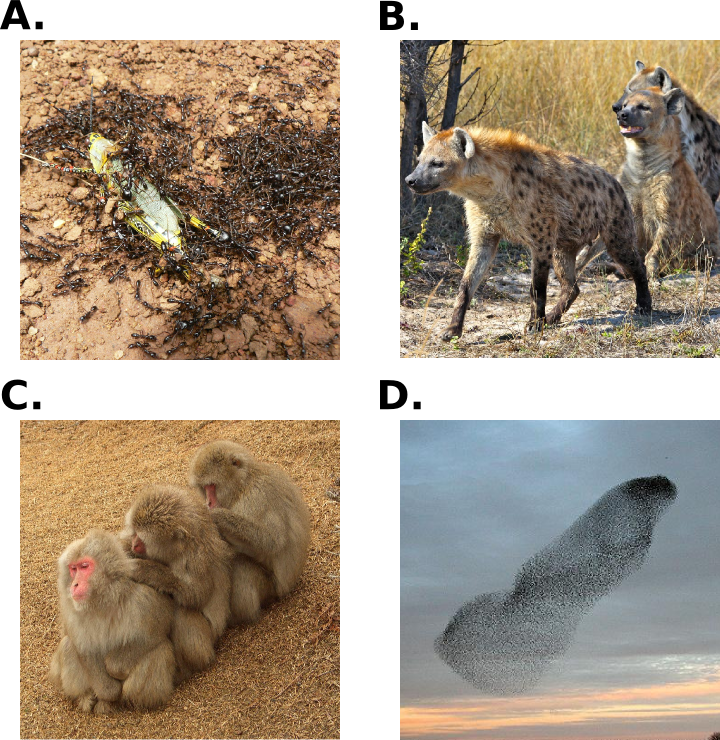
\includegraphics[scale = 0.5]{fig/Intro/CooperationExamples.png}
	        \caption{\textbf{La coopération à différents niveaux de complexité.} {\em (A)}~Les insectes eusociaux (comme les fourmis) possèdent une structure sociale extrêmement avancée. {\em (B)}~Les carnivores sociaux sont capables de coopération avancée ainsi que de se coordonner durant des chasses collectives. {\em (C)}~Le toilettage social est une activité durant laquelle les individus se toilettent à tour de rôle. {\em (D)}~Les volées d'oiseaux montrent l'émergence de déplacements collectifs d'une manière qui laisserait penser que les individus ne font partie que d'une seule entité.} 
	        \label{fig:CooperationExamples}
	      \end{center}
	  \end{figure}

		Un autre célèbre exemple de coopération est celui des insectes \emph{eusociaux}~\parencite{Wilson1990} (voir Figure~\ref{fig:CooperationExamples}~(A)). L'eusocialité est une forme extrême de société qui se retrouvent principalement chez les Hymenoptère (par exemple les fourmis, guêpes et abeilles) et Isoptère (notamment les termites). L'eusocialité est définie par des exemples avancés de coopération. En particulier, le soin des jeunes est pris en charge de manière collective par d'autres individus qui ne sont pas leur parents. Les animaux eusociaux font aussi généralement preuve d'une forme avancée de division du travail, où les individus se partagent une tâche en se répartissant en plusieurs rôles. Enfin, et c'est une des caractéristiques principales de l'eusocialité, il y a aussi une division de la reproduction. Ceci veut dire qu'il existe des castes reproductives et non-reproductives.

		Si nous dézoomons encore le niveau auquel nous observons le monde animal, nous pouvons nous intéresser aux comportements coopératifs des vertébrés. En particulier, les carnivores sociaux sont capables d'actions collectives poussées. Ces espèces sont notamment souvent connues pour leurs comportements de chasse collective où plusieurs individus sont capables de se coordonner afin d'attraper ensemble une proie qu'un individu seul n'aurait pu chasser. Les hyènes tâchetées (Figure~\ref{fig:CooperationExamples}~(B)) par exemple usent de signaux de communication avancés afin d'être capable de pouvoir chasser ensemble~\parencite{Drea2009a, Smith2010, Smith2012a}. Mais elles vivent aussi dans des groupes sociaux très organisés où les femelles sont en haut de la hiérarchie. Les femelles dominantes sont généralement les seules à se reproduire tandis que les femelles de rang inférieur s'occupent du soin des jeunes des dominantes. Nous pouvons aussi faire référence aux primates, qui ont des structures sociales très fortes. Ces derniers s'engagent notamment dans des du toilettage mutuel (voir Figure~\ref{fig:CooperationExamples}~(C)) entre différents individus du groupe~\parencite{Spruijt1992}.

		Enfin, à un niveau encore supérieur, nous pouvons citer les comportements de déplacement collectifs, par exemple des volées d'oiseaux (Figure~\ref{fig:CooperationExamples}~(D)). De manière, de nombreux animaux différents peuvent s'organiser en volée, troupeau ou bancs d'individus~\parencite{Couzin2002, Couzin2003}. Ces comportements d'agrégation ont de nombreux avantages pour le group tels qu'augmenter la confusion d'un prédateur, diminuer le risque d'un individu en particulier d'être attaqué ou se défendre de manière collective.


	\subsection{L'Évolution de la Coopération}

		Malgré l'omniprésence de la coopération dans le monde animal, expliquer son évolution est un des défi majeur en biologie évolutionniste.~\parencite{Hamilton1964, Dugatkin2002, West2011a}. En effet le principe de l'évolution tel que théorisé par Darwin peut être résumé par l'expression de la "survie du plus apte"~\parencite{Darwin1859}. Par conséquent, le comportement d'un individu ne peut être adaptatif que s'il lui est bénéfique. Plus précisément, le matériel génétique d'un individu se transmet lors de la reproduction. De là il ressort que, pour qu'un gène puisse se transmettre et donc se répandre dans la population, il est nécessaire qu'il permette à l'individu qui le possède d'augmenter sa capacité reproductive. Un trait particulier n'est donc adaptatif que s'il permet d'augmenter le nombre de descendants d'un individu (ce qu'on appelle valeur sélective).

		C'est sur ce point que l'évolution de la coopération semble être une contradiction. En effet, par définition, un comportement coopératif apporte un bénéfice à un autre individu. A partir de maintenant, lorsque nous ferons mention de bénéfices et coûts, nous nous référerons aux bénéfices et coûts à la valeur sélective des individus. C'est-à-dire que, lorsqu'un comportement est bénéfique à un individu, c'est qu'il permet \emph{au final} à cet individu d'accroître son nombre de descendants. Un comportement coopératif est donc un comportement qui augmente la valeur sélective d'un autre individu. Parfois même, coopérer est coûteux (d'un point de vue de la valeur sélective donc) pour l'acteur. C'est par exemple le cas pour notre exemple précédent des \emph{P. aeruginosas}, pour qui sécréter des nutriments est coûteux. Cet exemple peut nous servir à mieux illuster le problème posé par l'évolution de la coopération. Imaginons une situation où des organismes coopèrent et sécrètent donc des nutriments qui peuvent être utilisés par tous. Imaginons maintenant qu'un mutant apparaît aléatoirement dans cette population et que ce mutant possède un trait qui le pousse à tricher plutôt que coopérer. Il va donc profiter des nutriments sécrétés par les coopérateurs sans lui-même produire ces nutriments et donc en payer le coût. Par conséquent, sa valeur sélective sera supérieure à celle des coopérateurs. Il va donc pouvoir produire plus de descendants et son génotype de tricheur va pouvoir se répandre dans la population. Ceci va continuer jusqu'à que la population ne soit plus composée que de tricheurs. Il apparaît donc que la coopération ne devrait pas être stable. De nombreux modèles ont donc été proposés afin de définir des mécanismes pour expliquer l'évolution de la coopération. Ces mécanismes peuvent être majoritairement classés en deux catégories: les bénéfices \emph{directes} ou \emph{indirectes} à la valeur sélective~\parencite{West2007a}.

		Les bénéfices indirectes permettent notamment d'expliquer l'évolution de \emph{l'altruisme}. L'altruisme est un cas particulier de coopération dont nous avons précédemment parlé où coopérer est coûteux pour l'acteur du comportement coopératif~\parencite{Hamilton1964, West2007a}. Le comportement des \emph{P. aeruginosas} peut en effet être considéré comme altruiste. La division de la reproduction chez les insectes eusociaux, où seule une certaine caste d'individus peut avoir des descendants est aussi un exemple d'altruisme. Les individus non-reproducteurs paient en effect le coût maximal puisqu'ils ne possèdent pas de descendants du tout et ne peuvent donc pas transmettre leur matériel génétique. Il est donc difficile de comprendre comment un tel comportement peut être stable. Le mécanisme permettant d'expliquer l'évolution de l'altruisme a été proposé par Hamilton et s'appelle la \emph{sélection de parentèle}~\parencite{Hamilton1964}. Derrière ce terme est l'idée qu'un trait peut être transmis à travers les parents d'un individu. Si on considère en effet que l'unité de sélection est le gène, c'est-à-dire que l'évolution est due au fait qu'un gène permettant à un individu d'augmenter son nombre de descendants pourra ainsi se répandre dans la population, il n'est pas nécessaire que l'individu possédant ce gène se reproduise. En effet, s'il permet d'aider un individu qui est génétiquement proche de lui (un parent donc), il peut ainsi permettre à un gène permettant un comportement altruiste de se répandre aussi. La valeur sélective d'un trait n'est donc pas dépendante uniquement de la valeur sélective de l'individu possédant ce trait, mais aussi de celle de ces parents. C'est ce qu'on appelle la \emph{valeur sélective inclusive}. Ainsi un trait peut apporter des bénéfices indirectes en augmentant cette valeur sélective inclusive.

		Mais, tandis qu'un très grand nombre de travaux a été concentré sur l'évolution de l'altruisme et les bénéfices indirectes, la plupart des comportements coopératifs bénéficient directement à l'acteur. Dans ce cas, et l'acteur et le destinataire bénéficient du comportement coopératif. On parle aussi de comportement mutuellement bénéfiques pour cette catégorie de la coopération~\parencite{Bergmuller2007a}. Plusieurs mécanismes peuvent permettre d'expliquer comment la coopération peut-être adaptative grâce à des bénéfices directes. En particulier, ces bénéfices peuvent être forcés à travers de la réciprocité, des punitions ou encore des récompenses. Mais ces bénéfices peuvent aussi ne pas être forcés dans le cas où tous les individus partagent un intérêt à coopérer. Dans ce cas, on parle aussi parfois de \emph{bénéfices dérivés} afin de transmettre l'idée que la coopération peut-être dérivé d'un acte originellement égoïste. par exemple, faire partie d'un groupe plus grand d'individus permet d'augmenter les chances de survie (aussi bien face à l'environnement que contre des prédateurs) mais permet aussi de tirer des bénéfices plus importants de la chasse et de la récolte~\parencite{Clutton-Brock2002}. Une partie de la littérature sur la coopération mutuellement bénéfique s'intéresse aussi la coopération entre individus d'espèces différentes, ou coopération inter-espèces. Ceci s'appelle aussi du mutualisme (créant parfois une confusion avec le concept plus général de comportement mutuellement bénéfique). Par exemple, une certaine espèce de poissons, les Labres, sont connus pour le fait qu'ils nettoient d'autres poissons plus gros de leurs parasites et tissus morts. Mais de manière plus générale la coopération mutualiste intra-espèce est prédominante dans le monde animal. Et plus important, beaucoup de cas de coopération qui apparaissent altruistes à première vue sont en fait mutuellement bénéfiques. Par exemple, le Cratérope écaillé est un oiseau qui est connu parce que certains individus montent la garde et préviennent les autres de l'approche d'un prédateur, donnant ainsi l'impression qu'ils prenaient le risque d'être ainsi détecté par le prédateur en plus d'aider les autres à chercher de la nourriture. En véritié, le rôle de sentinelle est pris par des individus ayant déjà récolté suffisamment de nourriture et leur permet alors de maximiser leur propre survie dans un environment où les prédateurs sont nombreux~\parencite{Wright2001, Clutton-Brock2002}. Les comportement de coopération mutuellement bénéfiques sont donc cruciaux ainsi qu'à la base de la formation d'une structure sociale chez de nombreuses espèces.

		D'après ce que nous avons présenté précédemment, il pourrait apparaître que l'évolution de la coopération mutualiste est triviale. Et en effet, si on étudie uniquement le problème de la stabilité du comportement coopératif c'est le cas. Par exemple, comme expliqué avant, les comportements altruistes posent un problème de stabilité. Puisque ces comportements sont coûteux pour l'acteur, alors ils sont susceptible à l'invasion de tricheurs. Dans le cas des comportements mutuellement bénéfiques ce n'est plus le cas : puisqu'ils profitent à tous, un tricheur n'aurait aucun avantage à envahir la population. Cependant, ces comportements posent un problème d'évolution, c'est-à-dire d'essayer de comprendre comment ils ont pu se répandre dans la population à l'origine. Prenons l'exemple de la chasse collective comme c'est fait dans cette thèse. La chasse collective nécessite la coordination de plusieurs individus en même temps afin d'obtenir le bénéfice d'une chasse plus importante. Néanmoins, la nécessité de se coordonner un plus qu'il est compliqué d'amorcer la coopération. Pour le dire plus simplement, nous faisons face à un dilemme de la poule et de l'oeuf dans ce cas présent. Pour que la coopération soit sélectionnée, il faut qu'elle soit bénéfique. Or pour que la coopération soit bénéfique, les individus doivent être capable de se coordonner et donc doivent déjà avoir évolué la coopération. Il y a donc une question majeure sur la façon dont l'évolution de la coopération peut être amorcée.

		Plus généralement, ce problème est lié à la différence entre les explications proximales et ultimales~\parencite{Tinbergen1963}. Pour résumer rapidement, Niko Tinbergen a défini deux manières complémentaires pour étudier le comportement animale. Nous pouvons nous intéresser aux mécanismes du comportement afin d'obtenir les explications proximales ou nous intéresser aux conséquences en termes de valeur sélective ce qui correspond aux explications ultimales. Plus simplement, les mécanismes proximaux répondent au \emph{comment} et les explications ultimales répondent au \emph{pourquoi}. Afin de comprendre pleinement l'évolution des comportements, il est nécessaire de pouvoir répondre à ces deux questions. Or trop souvent, nous nous sommes surtout intéressés à explications ultimales au détriment des mécanismes proximaux. En particulier, les mécanismes de la coordination ont souvent été ignorés et simplement considérés comme une boîte noire. Par conséquent, la problématique à laquelle nous nous intéressons dans cette thèse est la suivante :
		\emph{l'influence des mécanismes pratiques des comportements de coordination sur l'évolution de la coopération mutualiste}.


\section{Méthodes}

	\subsection{Le Stag Hunt}

		Afin d'aborder ce problème, nous prenons inspiration sur les modèles de théorie des jeux évolutionniste~\parencite{MaynardSmith1973}. De manière générale, la théorie des jeux correspond à un ensemble de modèles utilisés pour étudier des dilemmes sociaux entre joueurs, notamment en économie. Le principe général est que généralement deux joueurs sont engagés dans une interaction pour laquelle ils peuvent adopter un ensemble de stratégie. Ces stratégies sont adoptées simultanément par les deux joueurs et chacun obtient une certaine récompense dépendant de sa stratégie et de celle de son adversaire. L'exemple le plus connu est celui du dilemme du prisonnier. Dans le cas de l'étude de l'évolution de la coopération, le cadre de la théorie des jeux a été repris pour former la théorie des jeux évolutionniste. L'idée est similaire à celle de la théorie des jeux classiques sauf que, plutôt que les joueurs soient des individus rationnels faisant toujours le meilleur choix pour eux-mêmes, on imagine cette fois que les joueurs sont simplement des individus qui évoluent. Ainsi, la stratégie jouée par chaque joueur dépend d'un processus d'évolution, permettant ainsi de représenter le problème de l'évolution de stratégies coopératives. Dans le cas de l'évolution de l'altruisme par exemple, il y a eu beaucoup de travaux autour du dilemme du prisonnier~\parencite{Axelrod1984}.

		Afin d'aborder les problèmes de coordination, il existe un modèle en théorie des jeux évolutionniste appelé le \emph{Stag Hunt} (la chasse au cerf)~\parencite{Skyrms2004}. L'idée de ce jeu est d'imaginer deux chasseurs ayant chacun le choix de chasser un lièvre ou un cerf. S'ils choisissent de chasser un lièvre, ils y arrivent forcément obtiennent une petite récompense. On considère généralement que les lièvres sont de plus en nombre tellement important qu'il n'y a pas de différence si un seul ou les deux individus chassent le lièvre. En comparaison, s'ils choisissent de chasser le cerf, alors il est nécessaire qu'ils le chassent tous les deux (donc qu'ils coopèrent) afin de réussir à le tuer. Ils obtiennent alors une récompense bien plus importante. Un résumé de ce jeu est présent dans la Figure~\ref{fig:} (il est à noter que les valeurs des récompenses n'ont que peu d'importance, seul leur ordre est vraiment important). Un point très important de ce jeu est qu'il contient deux \emph{équilibres évolutionnairement stables}: chasse au lièvre et chasse au cerf. Ce concept transmet l'idée qu'une fois ces équilibres évolués, ils sont stables. Par conséquent, ce jeu permet d'aborder le problème dont nous avons parlé précédemment : la stabilité de l'équilibre coopératif ne pose pas de problème mais la manière dont la coopération peut être amorcée n'est pas triviale.

    \begin{figure}[hbt]
        \begin{center}
          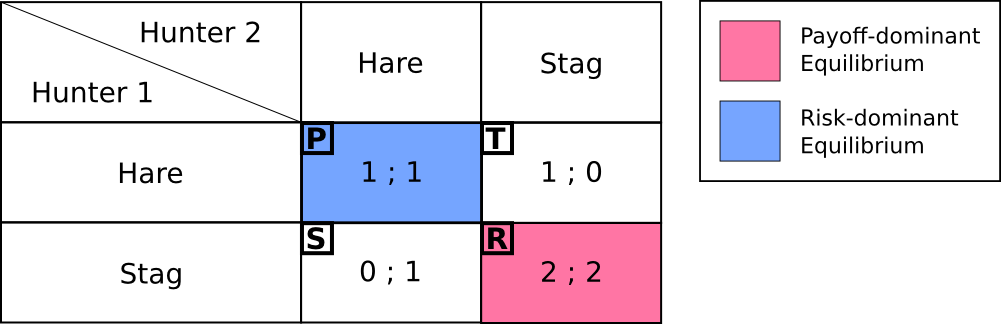
\includegraphics[scale = 0.50]{fig/Intro/StagHunt.png}
          \caption{\textbf{Matrice des gains de la chasse au lièvre.}
          Dans le jeu de la chasse au lièvre~\parencite{Skyrms2004}, on considère que durant une chasse, deux chasseurs peuvent soit chasser un lièvre ou un cerf. Chasser un lièvre peut être fait seul et assure l'obtention d'une récompense. En comparaison, chasser un cerf ne peut être fait que de manière coopérative mais rapporte plus qu'un lièvre. Par conséquent, un individu chassant un cerf seul n'obtiendrait aucune récompense. Les gains sont données de la manières suivante (Gain pour le chasseur 1; Gain pour le chasseur 2). Les valeurs exactes des gains n'ont pas d'importance tant que les différentes situations sont dans l'ordre suivant: R (récompense de la coopération) > T (tentation de tricher) = P (punition d'avoir triché) > S (sucker's payoff, c'est-à-dire la punition de s'être fait avoir). L'équilibre appelé "payoff-dominant" est l'équilibre où les chasseurs maximisent leur gain maximum tandis que l'équilibre appelé "risk-dominant" est celui où ils maximisent leur gain minimum.} 
          \label{fig:MatrixStagHunt}
        \end{center}
    \end{figure}


  \subsection{Robotique Evolutionniste}

    \begin{figure}[hbt]
        \begin{center}
          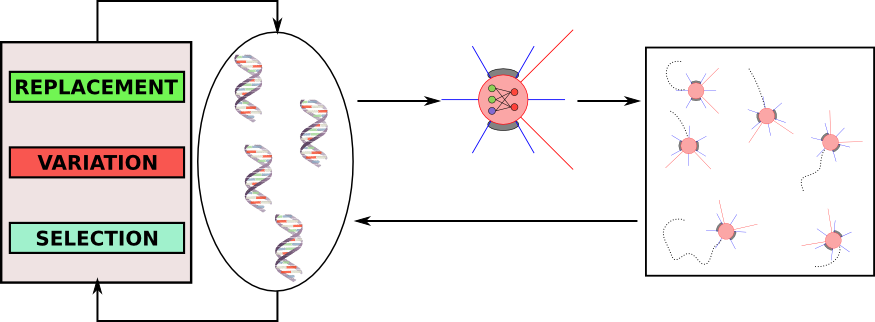
\includegraphics[scale = 0.50]{fig/Intro/EvolutionaryRobotics.png}
          \caption{\textbf{Fonctionnement général d'un algorithme de robotique évolutionniste.}
          Le but principal de l'ER est d'évoluer une population de génotypes. A cette fin, chaque génotype doit être évaluté afin d'obtenir un score de fitness. Un génotype est traduit en phénotype (ici un réseau de neurones artificiels) et ensuite intégré dans un robot afin d'agir en tant que contrôleur. Le robot situé dans son environment et son comportement est évalué en fonction des spécificités de la tâche. Une fois qu'on a assigné à chaque génotype un score de fitness, on utilise un algorithme évolutionniste. Cette phase sélectionne les génotypes jugés aptes à créer des descendants sur lesquels on applique de la variation. Finalement, cette nouvelle population de génotypes remplace la population précédente et le processus peut continuer pour une nouvelle génération.} 
          \label{fig:EvolutionaryRobotics}
        \end{center}
    \end{figure}

    Dans le contexte de cette thèse, le problème des modèles en théorie des jeux est qu'ils font des hypothèses que nous jugeons critiques sur les mécanismes proximaux. En particulier, il est généralement supposé qu'une mutation seul est suffisante pour évoluer un comportement coopératif pour un individu initialement non coopératif. Cela veut donc dire qu'une hypothèse est faite sur la disponibilité des mutations. Dans notre cas, puisque nous souhaitons étudier l'amorçace de la coopération mutualiste et le rôle de la coordination dans cette évolution, nous pensons que faire cette hypothèse masque l'influence des mécanismes proximaux sur l'évolution de la coopération. C'est pourquoi nous choisissons d'utiliser une méthode particulière pour aborder notre problème : la \emph{robotique évolutionniste} (ou ER).

    Le principe de la robotique évolutionniste est à la base de concevoir des robots en appliquant des concepts inspiré de l'évolution naturelle. Plus précisément, l'idée est d'appliquer des processus de sélection et de variation afin de pouvoir concevoir automatiquement des robots avec une approche holistique~\parencite{Nolfi2000, Doncieux2015a}. Le fonctionnement classique d'un algorithme d'ER est résumé dans la Figure~\ref{fig:EvolutionaryRobotics}. Concrètement, le but de l'ER est d'évoluer une population de génotypes. La forme exacte du génotype est extrêmement variable en fonction des travaux mais un choix courant est d'utiliser une liste de nombres réels. Ce génotype est alors transformé en un phénotype. Une fois encore, les formes des phénotypes sont très variables. Le point important est que ce phénotype est intégré dans un agent robotique (réel ou simulé) et permet de représenter le ou les traits du robot que nous souhaitons faire évoluer, que ce soit sa morphologie ou son contrôle. Par exemple, une implémentation courante de phénotype dans le cas du contrôle d'un robot est d'utiliser un réseau de neurones artificiels. Le robot est alors évalué dans un environnement afin d'accomplir une certaine tâche. Sa performance par rapport à cette tâche est ce qui détermine son score de fitness. 

    Une fois chaque génotype évalué vient l'étape de l'algorithme évolutionniste qui permet de créer la population de génotypes de la génération suivante. Pour celà on sélectionne d'abord les génotypes qu'on considère aptes à pouvoir se reproduire. Ces génotypes sont alors copiés afin de créer des descendants. Ensuite, on applique de la variation sur les descendants créés, ce qui peut consister en de la mutation ou de la variation. Une fois cette étape passée, ces génotypes constituent la population de la nouvelle génération et on peut entamer une nouvelle génération comme précédemment.

    Le point important de la robotique évolutionniste est qu'on évalue directement les phénotypes résultant de l'évolution des génotypes des individus. Cette technique peut donc être utilisée pour observer et étudier les comportements évolués ainsi que leurs intéractions avec un environnement aux conditions écologiques précises. En particulier, l'ER permet de faire le minimum de suppositions quand à la disponibilité des mutations et ainsi de pouvoir étudier en détail l'influence des mécanismes proximaux sur l'évolution de la coopération.


   \subsection{Setting Expérimental}

   	Maintenant que nous avons clairement posé nos hypothèses de travail, nous pouvons présenter notre setting expérimental. Nous choisissons donc de modéliser le problème de la chasse au cerf avec des techniques de robotique évolutionniste. Pour celà, nous étudions l'évolution de comportements coopératifs chez des agents robotiques \emph{simulés}. Chaque agent robotique est capable de mouvement et est équipé de deux type de senseurs différents. D'abord chaque agent est équipe d'une caméra frontale à $90$ degrés. Cette caméra permet de reconnaître le type de chaque objet (y compris les autres agents) qu'elle voit dans l'environnement ainsi que de renseigner sur leur proximité. Ensuite les agents possèdent aussi $12$ senseurs de proximités répartis tout autour de leur corps et qui permettent de ressentir les obstacles autour d'eux.

   	Chaque robot est contrôlé par un réseau de neurones artificiels. Ce réseau est un perceptron multi-couches avec une couche cachée et entièrement connecté. Les entrées du réseau sont constituées de l'ensemble des informations sensorielles de l'individu. Etant donné un ensemble d'entrées, le réseau de neurones permet de calculer deux valeurs de sortie qui correspondent aux vitesses respectives de chacun des deux roues du robot, permettant ainsi le déplacement.

   	L'environnement dans lequel évolue les robots est une arêne carrée entourée de $4$ murs. Cette arêne est remplie d'un certain nombre de proies qui peuvent être de types différents. Notamment, ces proies permettent de représenter les lièvres et cerfs qu'un chasseur peut chasser dans le modèle de la chasse au cerf. Tandis que ces proies sont immobiles, les agents robotiques peuvent se déplacer librement dans l'environnement. Afin d'attraper une proie, il est nécessaire pour un robot de rester au contact de cette proie pendant un temps prédéfini. Une fois ce temps passé, la proie est retirée et replacée à un endroit aléatoire de l'arêne afin de conserver la même proportion de proie durant toute une simulation. L'individu ayant chassé la proie reçoit alors une récompense dépendant de la proie et de si elle a été chassée de manière solitaire ou collective. Afin de chasser de manière collective, il est nécessaire aux deux individus de se trouver au contact de la proie au moment où elle est retirée de l'environnement. Ceci veut donc dire qu'il est nécessaire aux individus d'évoluer des comportements de coordination afin de pouvoir effectivement coopérer

   	Le génotype d'un individu correspond aux poids des connexions du réseau de neurones. Nous ne faisons pas évoluer la topologie du réseau. Afin d'évoluer les génotypes, nous utilisons un algorithme évolutionniste classique. L'évolution commence avec une population de génotypes initialisés aléatoirement. Afin d'évoluer chaque individu, cet individu est apparié avec un autre individu tiré aléatoirement dans la population. Ces deux individus sont alors évalués dans l'arêne présentée précédemment. Afin de diminuer les effets stochastique dus au placement initial aléatoire des proies, $5$ simulations indépendantes sont effectuées pour chaque paire. Afin que chaque individu rencontre un échantillon représentatif de la population, l'individu évalué est au total apparié avec $5$ individus différents. Une fois que tous les individus ont été évalués, les génotypes sont sélectionnés en fonction de deux processus de sélection différent selon l'expérience : une stratégie élitiste \((\mu+\lambda)\)-ES ou \emph{fitness proportionate}. Dans le premier cas, on parle de stratégie éliste car les meilleurs individus de la génération sont conservés pour la génération suivante. Plus précisément, on sélectionne les $\mu$ meilleurs individus (en terme de score de fitness) qui sont alors directement transférés dans la population de la prochaine génération. On crée alors $\lambda$ descendants à partir de ces $\mu$ meilleurs individus. Dans le cas du \emph{fitness proportionate}, le processus de sélection est plus proche du processus naturel de la sélection naturelle. En effet, afin de créer chacun des descendant constituant la nouvelle génération, on sélectionne aléatoirement parmi la population de parents (donc la population de la génération courante). Cependant, chaque parent a une probabilité plus forte d'être sélectionné si son score de fitness relatif par rapport aux autres individus de la population est plus élevé. Quelque soit la méthode de sélection, chaque descendant est un clone de son parent sur lequel on applique des mutations aléatoires. Ceci veut donc dire que nous n'utilisons pas de recombinaison.


\section{Modélisation de l'Evolution de la Coopération en Robotique Évolutionniste}

	\subsection{Motivation de la méthode}
	
		Dans une première partie de la thèse, nous sommes intéressé dans la modélisation computationnelle de l'évolution de la coordination. Plus particulièrement, nous souhaitons utiliser des outils de la robotique évolutionniste afin d'étudier l'influence des comportements de coordination dans l'évolution de la coopération mutualiste. En effet, comme expliqué dans l'introduction, les mécanismes proximaux ont souvent été ignoré quant à l'étude de ce type de comportement coopératif. Pourtant, ce sont ces mécanismes qui ont une influence sur la disponibilité des mutations vers la coopération. Plus précisément, nous pensons que dans les modèles classiques pour l'étude de l'évolution de la coopération, des hypothèses critiques sont faites et qui peuvent réellement changer la complexité de l'évolution des comportements collectifs.

		Nous choisissons d'utiliser de la robotique évolutionniste car cette méthode permet en effet de considérer en détail les explications pour proximales par rapport à d'autres méthode plus classique en biologie évolutionniste. Par exemple comme nous l'avons précédemment ditn une méthode très classique pour étudier l'évolution de la coopération est d'utiliser de la théorie des jeux évolutionniste. Cependant, dans ce type de modèles, il est souvent considéré qu'une mutation seule permet d'évolution la coopération pour un individu se comportant de manière solitaire. En pratique, l'évolution de la coopération sous-entend dans notre cas l'évolution de la coopération et donc d'un comportement complexe avant que des individus soient capables de récolter les bénéfices d'une action coopérative. Il est donc nécessaire d'utiliser une méthode qui nous permette d'étudier ces mécanismes avec précision.

		Pour celà, il est nécessaire de se tourner vers les méthodes de modélisation individu-centré (IBM)~\parencite{Huston1988}. Ces méthodes permettent de modéliser finement le comportement des individus et ensuite de s'intéresser à l'influence qu'ont les intéractions individuelles sur le comportement collectif. Ce type de modèles s'intéresse donc à la modélisation des variations individuelles et permettent ainsi de minimiser le nombre de suppositions faites à ce niveau-là~\parencite{Adami2014}. De ce fait, un certain nombre de travaux ont été intéressé dans la modélisation de phénomènes biologiques à l'aide d'IBM : de la formation des troupeaux~\parencite{Olson2013a, Haley2014, Olson2016} à l'évolution de l'altruisme~\parencite{Wilder2015} en passant par la symbiogénèse~\parencite{Watson1992}.

		Dans notre cas, nous pouvons considérer la robotique évolutionniste comme une instance particulière d'IBM. Les deux méthodes s'intéressent en effet à la modélisation des individus dans le but de l'étude d'une émergence collective. Un certain nombre de travaux en IBM utilise en fait le paradigme de l'ER. Mais le principal atout de l'ER par rapport aux IBM est le fait que l'individu est incarné~\parencite{Mitri2012} (un concept analogue à celui \emph{d'embodiment}). Les robots ont un corps physique ce qui rajoute un niveau supplémentaire d'intéractions. En comparaison, on fait parfois abstraction de ce genre de concepts en IBM. Or, l'embodiment peut justement avoir des effets inattendus et intéressants sur l'évolution de comportements collectifs~\parencite{Mitri2009}. Nous choisissons donc ici d'utiliser la robotique évolutionniste dans le but d'avoir ce niveau de modélisation supplémentaire et d'encore réduire le nombre de suppositions sur les mécanismes du comportement que nous faisons. Il est à noter que, même si de nombreux travaux récents se sont intéressés à l'utilisation de méthode ER pour la modélisation de l'évolution de la coopération~\parencite{Waibel2009, Waibel2011, Montanier2011, Ferrante2015}, l'évolution de la coopération mutualiste a en grande partie été ignorée de cette littérature.


	\subsection{Résultats}

		\subsubsection{L'Influence des mécanismes du comportement dans l'évolution de la coopération}

			Les premiers résultats présentés dans cette thèse sont centrés sur l'impact des mécanismes proximaux sur l'évolution de la coopération mutualiste. Ces résultats ont été publiés dans un journal international :

			\begin{quote}
			  \fullcite{Bernard2016a}
			\end{quote}

			Notre but est de montrer que les mécanismes des comportements de coordination sont critiques dans l'évolution des actions collectives. En particulier, nous nous intéressons à l'évolution des comportements mutuellement bénéfiques. Comme expliqué précédemment, les comportements mutualistes sont stables une fois qu'ils ont été évolués parce qu'ils bénéficient tous les individus. Cependant, leur amorçage n'est pas évident parce que ces comportements souvent requièrent l'évolution de la coordination. Par conséquence, un individu seul ne peut bénéficier de la coopération à moins que d'autres ne coopèrent aussi.

			Nous nous inspirons ici d'un modèle de théorie des jeux appelé le stag hunt~\parencite{Skyrms2004}. Nous pensons que des suppositions critiques sont faites dans les modèles classiques de théorie des jeux qui pourrait cacher la complexité d'évoluer des actions mutualistes. En particulier, il est généralement supposé qu'une seule mutation est suffisante pour évoler un individu coopératif à partir d'un individu solitaire. En réalité, l'évolution de la coopération implique l'émergence de plusieurs traits qui ne sont bénéfiques en eux-mêmes. Nous pensons ainsi que des contraintes mécanistiques critiques sur l'évolution de la coordination ont été négligées par ces modèles classiques. Afin de prendre ces mécanismes en compte, nous modélisons le stag hunt en robotique évolutionniste~\parencite{Nolfi2000, Doncieux2015}. Deux individus sont évolués dans une arêne fermée remplie de $18$ proies, la moitié d'entre elles étant des lièvres, l'autre moitié des cerfs. Chasser un lièvre rapporte moins que de chasser un cerf et peut être accompli de manière solitaire ou coopérative. En comparaison, les bénéfices de la chasse d'un cerf ne peuvent pas être obtenus à moins que les deux individus tuent la proie ensemble.

			Nous révélons alors qu'il existe des différences drastiques lorsque la transition vers la chasse au cerf est modélisée en robotique évolutionniste. En particulier, nous montrons que l'évolution de l'équilibre coopératif (la chasse au cerf) lorsque les individus agissent initiallement de manière solitaire (chasser au lièvre) apparait toujours avec un modèle en théorie des jeux classique. En comparaison, en robotique évolutionniste l'amorçage de la coopération est presque impossible puisque cette transition n'apparaît que dans $1$ réplicat sur $30$. De plus, même quand les individus sont génétiquement proches, la transition vers la coopération est toujours peu probable puisqu'elle n'apparait que dans 20\% de tous les réplicats. Notre modèles révèle ainsi que la transition vers la coopération est confrontée à un dilemme de l'oeuf et de la poule. Plus précisément, la coopération ne peut pas être sélectionniée à moins qu'elle soit bénéfique pour l'individu. Mais les bénéfices de la coopération ne peuvent être obtenus à moins que d'autres individus sont capable de coordination. En particulier, nous observons que l'évolution de la coordination implique l'émergence d'un comportement complexe qui a peu de probabilité d'évoluer par lui-même. Par conséquent, nous démontrons que les mécanismes pratiques de coordination ont un impact critique sur l'évolution de la coopération mutuellement bénéfique. Nous soutenons donc que les modèles considérant les expliquations proximales de la coopération sont critiques afin d'avoir une compréhension complète de l'évolution de la coopération mutualiste.


		\subsubsection{Optimisation des actions collectives par le biais de la sélection individuelle}

			Nous avons révélé à l'aide des résultats précédents que l'évolution des actions collectives était entravée par l'évolution de la coordination. En particulier, nous avons utilisé la robotique évolutionniste afin de mettre en lumière les contraintes mécanistiques qui agissent sur la transition d'un équilibre solitaire vers un équilibre coopératif. Notre intérêt a alors ensuite été de comprendre comment la sélection individuelle pouvait permettre la transition entre différents équilibres collectifs

			Les actions collectives permettent d'obtenir des bénéfices grâce aux intéractions de plusieurs individus. Même dans le cas où ces actions bénéficient à tous les individus de manière mutualiste, il n'est pas bien compris comment ces comportements collectifs sont atteint. Plus précisément, puisqu'ils requièrent la coordination de multiples individus, plusieurs équilibres évolutionnistes stables peuvent émerger. Mais, parce que les bénéfices sont obtenus par une action collective, un individu seul déviant de l'équilibre évolué ne serait pas adaptatif. Ceci veut dire qu'un mutant agissant vers un équilibre différent ne sera pas sélectionné, même si cet équilibre pourrait s'avérer plus avantageux pour le groupe. Par conséquent, ceci pose le problème de l'optimisation des actions collectives. A savoir, comment est-il possible pour la sélection individuelle d'amener à la transition vers un équilibre optimal quand un autre équilibre collective a déjà évolué.

			Un mécanisme classique pour résoudre ce problème est la sélection de groupe. Puisque ces comportements sont bénéfiques au niveau du group alors ceci impliquerait qu'ils sont sélectionnés au même niveau. Cependant, nous voulons étudier comment les comportements collectifs pourraient être optimisé par la sélection individuelle uniquement. A cette fin, nous choisissons de modéliser l'exemple de la chasse collective. En particulier, nous utilisons un modèle similaire à celui de nos précédents résultats. A savoir, des individus sont évolutés dans un environnement où ils peuvent chasser deux types de proies aux récompenses différentes: \emph{sanglier} et \emph{cerf}. Chaque type de proie correspond à un équilibre collectif différent: sous-optimal pour le sanglier et optimal pour le cerf. Notre but est ainsi d'étudier la transition de l'équilibre sous-optimal (chasse au sanglier) vers l'équilibre optimal (chasse au cerf).

			Nous montrons que sous des caractéristiques écologiques simples où seulement des proies sont présentes dans l'environnement, la transition vers l'optimum est impossible. Cependant, dans le contexte de suppositions plus réalistes où les individus doivent choisir entre plusieurs proies, alors l'équilibre optimal est évolué dans $8$ réplicats sur $30$. En particulier, les individus doivent même se coordonner afin de réussir à coopérer. Celà veut dire qu'ils doivent réagir au comportement de l'autre. De là il découle qu'ils réagissent aussi au comportement d'un mutant. Ceci permet donc en retour au groupe de bénéficier de la chasse au cerf.

			Cependant, dans la stratégie de coordination précédemment évolutée, les deux individus choisissent séparément quelle proie chasser. Nous étudions alors comment une stratégie de coordination plus asymétrique pourrait impacter la transition vers l'optimum. A cette fin, nous augmentons la complexité des réseaux de neurones contrôlant les individus afin de leur permettre d'évoluer des stratégies de coordination plus complexes. Dans ce cas, nous révélons que la transition vers l'optimum est facilitée puisque la chasse au cerf évolue dans $24$ réplicats sur $30$. De plus, nous observons l'évolution d'une stratégie asymétrique plus efficace où les individus adoptent deux rôles différents: la stratégie de \emph{leader/suiveur}. Dans cette stratégie, seul le leader décide de quel proie chasser le suiveur se content d'aller sur la même proie. Par conséquent, alors que choisir de coopérer sur un cerf était précédemment un problème de décision collective, il s'agit maintenant d'un problème individuel. Celà veut dire qu'un leader mutant allant vers un cerf est maintenant suffisant pour que les deux individus récoltent les bénéfices de la chasse au cerf. De plus, la stratégie de leader/suiveur a évolué parce qu'elle est plus efficace. Nous avons ainsi montrer que l'évolution d'une stratégie de coordination individuellement adaptative a mené vers l'optimisation d'un comportement collectif.



\section{Conception de Robots Coopératifs}

	\subsection{La Robotique Évolutionniste pour la Conception de Robots}

		Dans la seconde partie de la thèse, nous nous intéressons cette fois à la conception de robots coopératifs. Plus précisément, notre but est de s'inspirer de ce que nous avons appris grâce à nos résultats sur la modélisation biologique afin de permettre l'évolution de robots capable de coopérer. En particulier, nous voulons permettre l'évolution de la coopération entre robots hétérogènes.

		Les systèmes multi-robots (MRS) ont plusieurs avantages en comparaison d'un seul robot. Par exemple, ils peuvent permettre de résoudre plus facilement et/ou plus rapidement une tâche qu'avec un seul robot. Ils permettent aussi d'assurer plus de robustesse de la part du système puisque la présence de multiples robots peut être utilisé pour éviter que l'ensemble du système soit compromis suite à la panne d'un seul de ses élements. Il peut parfois aussi être plus rapide et moins coûteux de concevoir plusieurs robots aux capacités simples plutôt qu'un unique robot complexe. Mais concevoir un MRS est complexe. Il est en effet nécessaire d'être capable de concevoir le contrôle plusieurs robots dont on s'attend qu'ils fonctionnent simultanément. En particulier, de nombreuses caractéristiques de conception rentrent en compte dans la façon dont on va créer un MRS: centralisé/distributé, robots homogènes/hétérogènes, nombre de robots. 

		Les méthodes utilisées pour créer ces MRS dépendent principalement des choix fait à propos de ces caractéristiques architecturales. Depuis la création de ce domaine, de nombreuses méthodes ont été proposées, notamment afin de résoudre le problème du contrôle d'un MRS. Historiquement, les premières approches ont consisté à coder directement le comportement des robots afin d'obtenir le résultat désiré. Ceci a été très inspiré par les techniques appliquées sur des robots uniques et le but a souvent été d'adapter ces techniques pour plusieurs robots. Néanmoins, le contrôle d'un MRS est très différent d'un seul robot et souvent coder directement le comportement des individus devient beaucoup plus compliqué. Par exemple, il faut être capable d'anticiper l'émergence d'un comportement collectif à partir d'un ensemble de comportements individuels, impliquant beaucoup d'aller-retour afin d'arriver au comportement désiré.

		Il y a donc eu assez vite un intérêt pour utiliser des méthodes d'apprentissage afin d'automatiser la conception de MRS. Ainsi, de nombreux travaux se sont intéressés à utiliser de l'apprentissage par réinforcement (RL)~\parencite{Sutton1998}  dans ce but. Il existait déjà une grande littérature à ce sujet pour la conception automatique de robots seuls et là encore le but a été d'adapter ces techniques pour les MRS~\parencite{Gultekin2002, Bowling2003, Fernandez2005}. Mais appliquer des techniques d'apprentissage à plusieurs robots est complexe. En particulier, ceci implique souvent de simplifier le problème et d'utiliser des approximations afin d'être capable de pouvoir adopter ces algorithmes aux MRS.

		En comparaison, la robotique évolutionniste possède de nombreux avantages par rapport à l'apprentissage par renforcement. En particulier, il n'y a pas besoin d'estimer l'espace des états ce qui fonctionne très bien pour les problèmes en environnement ouvert et en boîte noire. Par conséquent, de nombreux travaux se sont intéressés à l'ER pour les MRS~\parencite{Watson2002, Brambilla2012, Hauert2014, Francesca2016}. En particulier, un problème intéressant pour la conception de MRS en ER est le fait de choisir entre des groupes de robots homogènes ou hétérogènes~\parencite{Waibel2009}. Des robots homogènes sont plus simple à évoluer puisque tous les robots bénéficient de la coopération. En comparaison, des équipes hétérogènes permettent d'avoir accès à une plus grande diversité de comportement entre les individus et donc potentiellement à des technique de coordination plus efficaces. Mais si les groupes sont hétérogènes alors ceci crée le problème de l'évolution de la coopération et du fait que des individus peuven agir de manière égoiste. Dans cette partie de la thèse nous nous intéressons donc l'évolution des comportements de coordination parmi un groupe de robots hétérogènes.

	\subsection{Résultats}

		\subsubsection{Le compromis entre évolvabilité et efficacité en robotique évolutionniste}

			Notre première étude dans cette partie de la thèse est concentrée sur l'évolution des comportements de coordination dans une tâche de récolte collective. Ces résultats ont été publié dans une conférence internationale :

			\begin{quote}
			  \fullcite{Bernard2015}
			\end{quote}

			Nous sommes intéressés par le sujet d'évoluer de la coopération parmi un groupe de robots hétérogènes. En particulier, nous souhaitons comparer une approche homogène (que nous appelons ici approche clonale) et une approche hétérogène. L'approche la plus classique pour concevoir des MRS en robotique évolutionniste est d'utiliser des groupes de robots homogènes. C'est en effet la manière la plus sûre de s'assurer de l'évolution de la coopération parce que la fitness des agents est la même que celle du groupe. Cependant, cela veut dire que nous nous concentrons souvent sur \emph{l'évolvabilité} de la coopération, c'est-à-dire la probabilité d'évoluer des individus coopératifs~\footnote{Il est important de préciser que le term "évolvabilité" a une forte connotation dans le domaine de la robotique évolutionniste et qu'il peut correspondre à plusieurs définitions. En particulier, une de ces définitions est que l'évolvabilité représente la capacité pour un individu de s'adapter aux changements dans l'environnement~\parencite{Wagner1996}. Il s'agit d'un sujet prometteur en évolution artificielle~\parencite{Banzhaf2006, Lehman2013, Doncieux2015a, Taylor2016} et par conséquent nous ne voulons pas créer de confusion quant à notre utilisation du terme. Dans cet article, l'évolvabilité fait uniquement référence à la capacité d'évoluer un trait particulier (dans notre cas la coopération)}. Cependant des groupes de robots hétérogènes peuvent permettre d'atteindre une plus grande \emph{efficacité} (en terme de fitness) quand de la coordination est nécessaire. Parce que les individus peuvent adopter des comportements distincts, ils peuvent évoluer des stratégies de coordinations plus diverses. Mais la présence d'hétérogénéité peut aussi gêner l'évolution de la coopération dans un environnement où il est possible pour les robots de se comporter de manière égoiste. Nous voulons ainsi comparer ces deux approches dans ce genre d'environnement sur la base de deux critères : évolvabilité et efficacité.

			A cette fin, nous avons conçu une tâche de recolte collective inspirée par le stag hunt. Plus précisément, deux individus sont placés dans une arêne où ils peuvent collecter deux types différents de ressources : vert et violet. Les ressources vertes rapportent autant qu'elles soient collectées de manière solitaire ou collective. En comparaison, les ressources violettes doivent être collectées coopérativement mais rapportent plus que les vertes. Etant donné cette tâche, nous étudions l'évolution de comportements coopératifs, c'est-à-dire quand les individus collectent ensemble des ressources violettes. Nous étudions trois compositions de groupes différentes :

			\begin{itemize}
			  \item{Contrôle, où les individus viennent de la même population mais sont génétiquement différent.}
			  \item{Clonal, où les individus sont des clones l'un de l'autre.}
			  \item{Coévolution, où les individus viennent de populations différentes.}
			\end{itemize}

			Nous comparons alors les résultats de deux approches hétérogènes (contrôle et coévolution) et d'une approche clonale sur les deux critères présentés précédemment.

			Nous révélons qu'il existe un compromis entre évolvabilité et efficacité dans notre tâche de récolte. En particulier, l'approche clonale donne les meilleurs résultats pour ce qui est d'évoluer des individus coopératifs. En comparaison, l'approche en coévolution permet l'émergence de comportements coopératifs plus efficaces. De plus, on observe, dans l'approche en coévolution, l'évolution de division du travail par le biais d'une stratégie de \emph{leader/suiveur}. Nous souhaitons alors dépasser ce compromis et améliorer chacune des approches sur les deux critères d'évolvabilité et d'efficacité.

			Pour celà, nous utilisons de l'évolution incrémentale. Les individus sont d'abord pré-évolués dans un tâche de coopération plus simple où ils ont un traversé un ensemble de points de passage. Les individus sont récompensés par le fait de traverser les mêmes points de passage dans le même ordre. Après ça, ces individus sont évolués dans la tâche de collecte présentée précédemment. Nous montrons que, bien que la probabilité d'évoluer la coopération augmente sous coévolution, aucun différence significative n'est observée avec l'approche clonale. Ceci veut alors dire que l'approche en coévolution atteint les meilleurs scores d'évolvabilité \emph{et} d'efficacité comparé aux autres approches. Nous montrons alors qu'il existe un nouveau compromis : il est possible d'améliorer l'évolvabilité de stratégies de coordination efficaces mais au coût de temps computationnel supplémentaire.


		\subsubsection{L'évolution de la spécialisation dans une population de robots hétérogènes}

			Nous étudions maintenant l'évolution de la division du travail entre des robots hétérogènes par le biais de polymorphisme génotypique. Ces résultats ont été publié dans une conférence internationale :

			\begin{quote}
			  \fullcite{Bernard2016b}
			\end{quote}

			Nous avons précédemment montré qu'il pouvait être bénéfique de considérer la qualité des comportements de coopération en plus de la probabilité d'évoluer la coopération. En particulier, nous avons montré qu'une approche hétérogène particulière, la coévolution coopérative, permettait l'émergence d'une stratégie de coordination plus efficace: leader/suiveur. Ce comportement implique l'évolution de spécialisation (ou division du travail). Ici nous nous intéressons à l'évolution d'une stratégie de leader/suiveur dans une seule population d'individus

			Puisque la coopération est souvent atteinte entre robots homogènes en robotique évolutionniste, alors pour permettre de la division du travail, les individus doivent être capable d'adapter leur phénotype durant leur vie. Par conséquent, la spécialisation repose sur de la plasticité phénotypique ou des indices environnementaux. Ici nous nous sommes intéressés à l'évolution de la spécialisation sans ces mécanismes supplémentaires. Ceci veut dire que nous voulons créer de la division du travail au niveau de la population. Par conséquent, nous voulons étudier le maintien de plusieurs génotypes différentes codant pour différent rôles dans une unique population, c'est-à-dire du polymorphisme génotypique. En particulier, nous nous concentrons sur l'impact des méthodes de séléction sur l'évolution du polymorphisme génotypique.

			A cette fin, nous utilisons une tâche de récolte plus simple que celle utilisée précédemment. Deux individus génétiquement différent sont placés dans une arêne où ils peuvent récolter un seul type de ressource. Cette ressource est plus intéressante si elle est récoltée de manière coopérative. Ceci veut dire qu'évoluer la coopération est simple (ce n'est pas le sujet ici) et que l'accomplissement de la tâche est favorisé par l'évolution de stratégies de coordinations efficaces. Comme montré précédemment, deux stratégies de coopération différentes peuvent évoluer ici. D'un côté, il y a la stratégie des \emph{tourneurs}, où les deux individus adoptent le même comportement afin de se coordonner. Il s'agit donc d'une stratégie généraliste. D'un autre côté, ils peuvent aussi évoluer des comportements de spécialistes et adopter une stratégie de leader/suiveur. Nous nous intéressons à l'étude des différences évolutionnaires de deux méthodes de sélection différentes: (1) un \((\mu + \lambda)\)-ES (sélection élitiste) et (2) une sélection fitness-proportionate. Nous étudions aussi l'impact de la taille de la population.

			Nous révélons que la spécialisation est presque impossible à évoluer quand une sélection élitiste est utilisée. En effet, dans un seul réplicat sous grande taille de population nous observons la présence de spécialistes dans la population à la fin de l'évolution. De manière surprenante des spécialistes apparaissent néanmoins dans plusieurs réplicats mais ne sont jamais maintenus. Même lorsque la population est initialisée avec des spécialistes des résultats similaires sont observés. En comparaison, tandis que les spécialistes ne sont presque jamais évolués en sélection fitness-proportionate, ils sont facilement maintenus durant l'évolution (en particulier quand la population est initialisée avec des spécialistes). Nous révélons ainsi que l'évolution de polymorphisme génotypique est gênée par le défi à la fois d'évoluer et de maintenir des spécialistes dans la population et qu'aucune de nos deux méthodes de sélection n'est appropriée pour celà.

			Nous utilisons alors des analyses computationnelles afin de mieux comprendre les mécanismes sous-jacent à ce problème. Nous montrons que bien que les spécialistes soient les plus efficaces, les généralistes peuvent envahir la population parce qu'ils ont de bons résultats contre n'importe quel phénotype. En comparaison, les spécialistes ont besoin d'être appariés avec d'autres spécialistes d'un type différent pour avoir de très bons résultats. Des analyses complémentaires montrent que, sous une taille de population finie, la diversité génétique peut être perdue d'une génération à l'autre. Nous révélons ainsi deux propriétés critiques pour l'évolution du polymorphisme génotypique: (1) la protection contre l'invasion de généralistes et (2) la maintenance de la diversité génotypique. Nous pensons qu'un algorithme possédant ces propriétés pourrait permettre d'obtenir du polymorphisme génotypique.


\section{Conclusions}

	\subsection{Contributions}

		Dans cette thèse nous avons abordé le sujet de l'évolution de la coordination en robotique évolutionniste. Pour cela, nous avons pris deux approches différentes liées à la robotique évolutionniste~\parencite{Nolfi2000, Doncieux2015a} : la modélisation et la conception~\parencite{Trianni2014b}.

		Pour la première approche, nous nous sommes intéressés à modéliser l'évolution de la coopération mutualiste en robotique évolutionniste. Plus précisément, nous avons utilisé des outils de cette méthode afin de pouvoir étudier l'influence des mécanismes proximaux de la coordination dans l'évolution de la coopération. Pour celà, nous avons pris inspiration du modèle de théorie des jeux du stag hunt~\parencite{Skyrms2004} où des individus peuvent choisir de chasser des lièvres de manière solitaire ou de coopérer pour chasser des cerfs qui sont plus intéressants pour eux. Nous avons tout d'abord montré qu'en utilisant une méthode en robotique évolutionniste, il était possible d'observer des différences drastiques avec des modèles classiques de théorie des jeux. Notamment, alors qu'avec un modèle classique l'évolution de la coopération (chasse au cerf) était facile, elle est presque impossible avec une modélisation en ER. En particulier, nous montrons que l'évolution de la coopération suppose l'évolution de comportement de coordination complexes qui n'ont que peu de chance d'évoluer seuls. Notamment, la coordination ne peut pas être bénéfique tant que les individus ne coopèrent pas et vice versa. Nous révélons donc que, grâce à une méthode de modélisation en robotique évolutionniste, il est alors possiblede mesurer plus finement l'impact des mécanismes pratiques du comportement sur l'évolution de la coopération.

		Nous nous sommes alors intéressés à l'optimisation d'actions collectives. En particulier, nous voulions étudier comment la sélection individuelle pouvait permettre la transition d'un comportement collectif sous-optimal à un comportement collectif optimal. A première vue en effet, ce problème d'optimisation, parce qu'il concerne un comportement de groupe, ne devrait pouvoir être résolu que par le biais de la sélection de groupe. Nous montrons alors qu'il est possible d'atteindre l'optimum grâce à la sélection individuelle uniquement. En particulier, nous révélons que la coordination, parce qu'elle permet de réagir au comportement d'autres individus, permet aussi de réagir au comportement de mutants et donc ainsi de permettre de modifier indirectement le comportement du groupe. La nature de cette coordination change aussi la facilité avec lequel cette action collective est optimisée. Ainsi, nous montrons aussi que lorsque des comportements de coordination asymétriques sont évolués, alors la transition vers l'optimum est grandement facilité. Ces stratégies asymétriques sont de plus sélectionnées uniquement parce qu'elles sont plus efficace pour les individus. La sélection individuelle est donc suffisante pour expliquer l'optimisation d'un comportement collectif.

		Puis, dans le cadre de la deuxième approche, nous avons alors étudié la conception automatique de système multi-robots grâce à la robotique évolutionniste. En particulier, nous nous sommes intéressés à l'évolution de robots coopératifs dans une tâche nécessitant de la coordination et quand les robots faisaient parti d'un groupe hétérogène. Dans un premier temps, nous avons comparé des approches homogènes et hétérogènes et montré que, dans un environnement où il était possible d'avoir des comportements égoistes, l'approche homogène permettait d'évoluer plus facilement la coopération. Cependant, avec une approche hétérogène (la coévolution dans ce cas), il était possible d'évoluer des stratégies de coopération plus efficace et notamment de la division du travail. Nous révélons ainsi l'exitence d'un compromis entre évolvabilité et efficacité. En utilisant de l'évolution incrémentale, nous sommes capable de dépasser ce compromis en augmentant la probabilité d'évoluer des stratégies coopératives parmis un groupe hétérogènes. Nous créons cependant aussi un deuxième compromis. En effet, il est possible d'augmenter l'évolvabilité de l'approche hétérogène mais en contrepartie il est nécessaire de payer un surcoût computationnel.

		Enfin, nous nous sommes finalement intéressés à l'évolution de polymorphisme génotypique au sein d'une population de robots. Plus précisément, nous avons étudié l'évolution de la division du travail au sein d'un groupe hétérogène de robots en fonction de la méthode de sélection de l'algorithme évolutionniste. Nous avons alors montré que, sous une sélection élitiste il était presque impossible de maintenir des spécialistes dans la population mais facile de les évoluer. En contrepartie, sous une sélection fitness-proportionate, le maintien de ces spécialistes était facile mais leur évolution difficile. Par le biais d'analyses computationnelles, nous avons pu montrer que les généralistes pouvaient envahir la population et remplacer les spécialistes parce qu'ils ne nécessitaient pas de se retrouver avec un phénotype particulier afin de pouvoir accomplir la tâche efficacement. De plus, des analyses supplémentaires ont montré que la taille de la population était nécessaire au maintien de la diversité génétique. Ainsi, nous avons révélé des propriétés critiques qui pouvaient permettre de concevoir un algorithme capable d'évoluer du polymorphisme génotypique.


	\subsection{Perspectives}

		D'un point de vue de la modélisation de la coopération, cette thèse ouvre des perspectives intéressantes que aurions souhaité étudié en détail. En particulier, l'évolution de la communication représente un sujet majeur dans l'étude des comportements sociaux. Il serait ainsi possible d'étudier comment des individus pourraient évoluer d'eux-mêmes des capacités de communication et comment la communication pourrait alors influer l'évolution de la coopération. 

		Pour ce qui est de la conception de systèmes multi-robots, une perspective serait d'étudier l'évolution de la coopération sous d'autres conditions. Tout d'abord, toutes nos expériences ont été effectuées sur des robots simulés. Il pourrait être intéressant de voir si nos comportements évolués en simulation pourraient être facilement transférables sur des robots réels. Ceci permettrait de valider que nos simulations ne font aucune supposition critique sur la modélisation de l'environnement qui empêcherait d'obtenir les mêmes résultats dans le monde réel. Une autre perspective intéressante serait de changer de paradigme et d'étudier l'évolution de la coopération dans un contexte en-ligne et dirigé par l'environnement~\parencite{Montanier2011, Montanier2013}. Dans ces conditions, les robots sont directement évolués dans l'environnement et il n'y a pas de phase séparée de conception et de production. De plus, lorsque l'évolution est dirigée par l'environnement la fonction de fitness n'est plus donnée directement mais naît de la nécessité de rencontrer d'autres individus afin de pouvoir créer descendants. Ceci pourrait avoir des conséquences intéressantes pour l'évolution de l'évolution de la coopération.

\chapter{General Introduction}

\epigraph{\textit{Natural selection cannot possibly produce any modification in any one species exclusively for the good of another species.}}{--- \textup{Charles Robert Darwin}}

\minitoc[n] % minitoc without title

% We will volontarily be vague at time. Please bear with us

\section{The Evolution of Cooperation}

  \subsection{Cooperative Behaviours and their Significance in Evolutionary History}

    % Peut-être que je m'épanche un peu trop là quand même

    \subsubsection{The abundance of cooperation} 

    % Mentionner les major transitions

    In particular, its examples and practical occurences are as diverse as central in numerous species. As we will see in the next Subsections, many different definitions of what really constitutes a cooperative behaviour exist (TODO: en fait non pas vraiment, plutôt dire que ya des précisions importantes en plus de la définition qu'on va donner là). In our case, we will choose the classical one in evolutionary biology: cooperation is a behaviour where an \emph{actor} (the individual who initiates the behaviour) behaves in such a way that is beneficial to a \emph{recipient}~\parencite{West2007a}. Given how broad this definition is, numerous diverse biological phenomena can be included under this label. 

    Cooperation is prevalent at every level of the natural world. Even unicellular organisms such as bacteria and microorganisms are known to frequently act in a cooperative manner. By using secreations, microroganisms are capable of collective sharing and communication~\parencite{Elena2003, Keller2006, West2006}. \emph{Pseudomonas aeruginosas} for example produce nutrients that every organism in the vicinity can benefit from~\parencite{Popat2012, Harrison2013}.

    However, this also means that some organisms could profit from these nutrients without having to produce anything themselves (given that production is costly). This is where a problem of public goods can arise: because "cheaters"\footnote{The term "cheaters" will appear several times along the lines of this manuscript. Because this word has a particular bad connotation with regards to human actions, it may be misunderstood that we attribute a malevolent intention to the organisms. Rather, through the rest of the manuscript, It should be understood as "one that profits from a benefit without paying any cost".} can benefit from these nutrients without contributing themselves. Interestingly, these situations are well studied in the realm of cooperative dilemma, as in economics for example.
    
    
    , which proves how complex these cooperative interactions in microorganisms are. It would also not be so far-stretched to consider that the complex network of genes interactions, where genes act together to build complex living machines may very well fall under the umbrella of cooperation. It is even more astonishing when we consider that those genes used to be independent replicators living freely~\parencite{Dawkins1976, Szathmary1995}. Finally, and in a similar fashion as our previous example, multicellularity is a perfect display of high cooperation between numerous different organisms. The birth of multicellular organisms is explained by the fact that single prokaryotic organisms gathered and where incorporated as mitochondries in what are now eukaryotic cells to form complex multicellular organisms. Szathmary \& Maynard Smith considered this cooperative transition to multicellularity as one of the major transitions in evolution~\parencite{Szathmary1995}.

    \begin{figure}[hbt]
        \begin{center}
          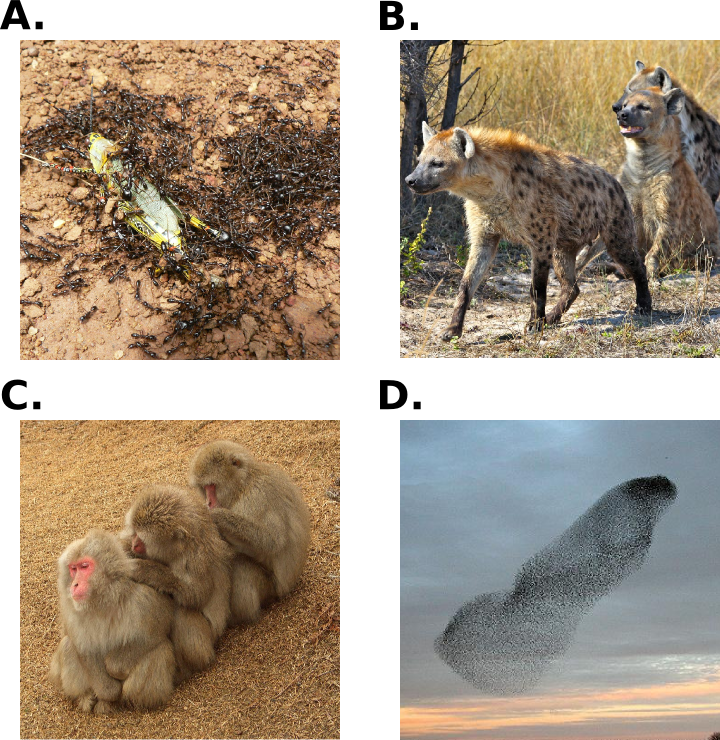
\includegraphics[scale = 0.5]{fig/Intro/CooperationExamples.png}
          \caption{\textbf{Cooperation at every level of complexity.} {\em (A)}~Eusocial insects like Hymenoptera (e.g. ants) are capable of impressive collective behaviours. {\em (B)}~Social carnivores exhibit strong cooperative behaviours and are capable of great feats of coordination during collective hunts. {\em (C)}~Social grooming is a social behaviour where individuals will groom each other reciprocally. It is thought to be a bonding exercise whose ultimate goal is to strengthen the social structure of the group. {\em (D)}~Flocks of birds are signs of the emergence of collective motions as if every individuals were part of a single bigger entity.} 
          \label{fig:CooperationExamples}
        \end{center}
    \end{figure}

    Much higher on the size scale is a popular textbook example of social behaviours: ants~(Figure~\ref{fig:CooperationExamples}~(A)). More generally, the presence of \emph{eusociality} in the animal world is an astonishing display of cooperative features~\parencite{Wilson1990}. While ants are among the most well-known examples, insects from the Hymenoptera (i.e. ants, wasps, bees) and Isoptera (i.e. termites) orders are all eusocial and represent most of the insect biomass\parencite{Wilson2008}. It is interesting to note that two rodent species, the naked mole-rat and the Damaraland mole-rat, are the only vertebrates to have achieved eusociality. Eusociality might be defined as one of the highest levels of sociality and displays several impressive examples of highly advanced cooperative actions. For example, there is cooperative care of youngs in eusocial societies, which means that individuals help raise offsprings which are not their own. Also, eusocial insects are capable of achieving efficient division of labour, a cooperative trait where individuals specialize between several roles, either to achieve several tasks simultaneously or to coordinate more efficiently. In particular, division of labour is often permanent and comes with strong morphological differences between specialized individuals. Last but not least, eusociality is also defined by the division of reproductive labor. This means that there exists reproductive and non-reproductive castes (e.g. the worker caste), which is an extreme form of cooperation between these individuals. Because of all of these reasons, an ants colony is often viewed as a particular superorganisms wherein individuals work as one for the benefit of the group.

    If we unzoom again the lens with which we look at the world, we can find other powerful examples of cooperation among bigger vertebrates. Numerous species have evolved strong sociality, or presociality, which gives the opportunity to watch impressive cooperative actions in the animal world. For example, social carnivores are capable of collective hunting, where several members of the same group will coordinate their actions to catch a particularly difficult or quick prey. For examples, lions are famously known for their communal and highly cooperative behaviours of collective hunting, for which they are capable of division of labour~\parencite{Scheel1991, Stander1992}. Less well-known but as much impressive, spotted hyenas~(Figure~\ref{fig:CooperationExamples}~(B)) also demonstrate high level of coordination in their collective hunting habits. While often wrongly considered but a scavenger, hyenas are also great hunters who rely on signaling and communication to coordinate~\parencite{Drea2009a, Smith2010, Smith2012a} and are capable of defending their catch against lions. The behaviours of those predators could easily be considered as complex tactics by a human observer. But even without being concerned with something as brutal as hunting, social carnivores tend to live, as their name suggests, in highly cooperative societies. To go on with the example of spotted hyenas, they are in particular considered to be the most social among Carnivora~\parencite{Mills2003} and the complexity of their social organization is comparable to that of primates~\parencite{Drea2003}. They live in a matriarchal societies where the females dominate the males and enforce the hierarchy through agression. Non-dominant females also take care of the youngs of other females higher in the hierarchy, something which is known as alloparenting and can also be found in primates~\parencite{Small1990} and in other carnivores~\parencite{Packer2001}. Among several social species, individuals also engage in social grooming~(Figure~\ref{fig:CooperationExamples}~(C)), where they will clean each other and which is an important bounding activity which strengthen the social structure of the group~\parencite{Spruijt1992}. Finally, we can also quickly mention the behaviours of sentinels, for example in birds like the Arabian babbler~\parencite{Wright2001} or meerkats~\parencite{CluttonBrock1999}. Individuals who adopt these behaviours will act as watchers for other individuals in their group, responsible for looking for predators approaching and warn the other individuals, sometimes thus taking the risk of attracting attention to themselves.

    It is also easy to be amazed by the collective motion of flocks of birds~(Figure~\ref{fig:CooperationExamples}~(D)). Animals might sometimes organize into flocks, herds or schools from which will emerge a collective behaviour~\parencite{Couzin2002, Couzin2003}. In particular, what is impressive is that the collective cohesion achieved is due to individual behaviours which do not depend on high cognitive abilities and does not require a particular central decision. These social behaviours are beneficial to the individuals that constitute the groups because it can for example increase group vigilance, confuse predators, decrease the risk for each individual to be attacked or even allow to organize an active defense against a predator~\parencite{Hamilton1971, Olson2013}.

    For the moment we simply gave examples of cooperation between members of the same species (intraspecific cooperation). Yet if we again look at a higher scale we can also observe numerous displays of cooperation between individuals of different species (interspecific cooperation). Often called mutualism (as we explain later), this form of cooperation is abundant~\parencite{Bshary2004}. For example, most plants require pollinators in order to transport their pollen so that they can succesfully pollinate the flowers. In exchange, the pollinators, whose most representative are insects, gain nectar as a benefit. Another example is that of cleaning symbiosis, where a "client" has its teeth or body cleaned from parasites or dead tissues by another smaller "cleaner"~\parencite{Poulin1996}. For example, some fishes, especially wrassers, are known to often clean other bigger fishes, to the point that there exists "cleaning station" where multiple aquatic animals converge to enjoy their services. The yellow-billed oxpecker also regularly eats insects and ticks from the back of mammals. The gut flora of some animals, human beings among them~\parencite{Backhed2005}, is also another example of strong interspecific cooperation, as it is constituted of up to 100 trillion of microorganisms that help process food.

    % KILLER WHALES ? Domestication ?

    % On peut en dire plus sur les humains mais j'ai pas les références pour le moment.

    In conclusion, in nearly every different levels of complexity in the living world, we can find examples of cooperative actions. More importantly, cooperation is not only present but also appears to be one of the leading factors in every major transitions in evolution~\parencite{Szathmary1995}. Moreoever, we did not touch upon human cooperation until now but it is obvious that human beings are very strong cooperators. In particular, cooperation is at the basis of the construction of our social structure and social sciences have been for long interested in studying human cooperation~\parencite{West2011a}. Therefore there is particular interest in trying to explain how could cooperation evolve and give rise to so much diversity in social behaviours today. 


    \subsubsection{Evolving cooperation} 

    Yet explaining the evolution of cooperation has been one of the major challenges in evolutionary biology~\parencite{Hamilton1964, Dugatkin2002, West2011a}. Charles Darwin, as shown by the epigraph of this chapter, had already figured that the evolution of cooperation could pose a problem to his theory. In particular, he thought that the existence of a non-reproductive caste in eusocial insects was "one special difficulty, which at first appeared to me to be insuperable, and actually fatal to my whole theory"~\parencite{Darwin1859}. 

    Based on the theory of evolution, life is a struggle where only the \emph{fittest individuals} survive. The main purpose of evolutionary biology is to explain adaptation~\parencite{West2011a}. In particular, natural selection is driven by the reproduction of individuals. Namely, because transmission of genetic material occurs through reproduction, evolution leads to an increase in genes and traits that increase the relative number of offsprings (i.e. fitness) of the organism. This is where this understanding of adaptation appears to contradict the evolution of cooperation.

    % For example, a individual that acts as a sentinel for the group takes the risk of being spotted more easily by a predator, thus paying a hefty cost for the good of the others.

    % However, this also means that some organisms could profit from these nutrients without having to produce anything themselves (given that production is costly). This is where a problem of public goods can arise: because "cheaters"\footnote{The term "cheaters" will appear several times along the lines of this manuscript. Because this word has a particular bad connotation with regards to human actions, it may be misunderstood that we attribute a malevolent intention to the organisms. Rather, through the rest of the manuscript, It should be understood as "one that profits from a benefit without paying any cost".} can benefit from these nutrients without contributing themselves. Interestingly, these situations are well studied in the realm of cooperative dilemma, as in economics for example.


    Cooperation is defined as a behaviour that benefits another individual than the actor. Please keep in mind that "costs" and "benefits" refer to the fitness of the individual (i.e. the number of this individual's offsprings) and not direct material elements. In consequence, it decreases the relative fitness of the actor compared to that of others in the population and should then be selected against. In particular, cooperative individuals are under the threat of invasion from cheaters (or freeloaders\footnote{The terms "cheaters" and "freeloaders" will appear several times along the lines of this manuscript. Because this word has a particular bad connotation with regards to human actions, it may be misunderstood that we attribute a malevolent intention to the organisms. Rather, through the rest of the manuscript, It should be understood as "one that profits from a benefit without paying any cost".}). To illustrate this issue, let us take back the example of \emph{P. aeruginosas} which we previously talked about. Let's image a population constituted of cooperators which thus can pay a certain cost to give a benefit to others. A given individual can benefit from every individuals in the population and the situation appears ideal. However, say now that a mutant, which does not cooperate, appears in the population. Then this mutant can benefit from the cooperative actions of others without having to pay any cost. From this it stems that its relative fitness will be higher than that of the other individuals. In consequence, it will produce more offspring and mutants will begin to invade the population. The process will repeat itself as cheaters always have a higher fitness than cooperators until no cooperators are left in the population. From this comes that cooperation should not be able to exist. 

    Biologists have therefore been studying the mechanisms which could explain the evolution of cooperation for several decades. Because cooperative actions are so diverse, numerous models have been proposed to classify the different mechanisms which could explain the adaptation of cooperative traits (we direct an interested reader to a few of them~\parencite{Dugatkin2002, Keller2006, Bergmuller2007a, West2007}). For our overview of cooperation in this present manuscript, we follow the classification of West and colleagues~\parencite{West2007a}. In particular, these mechanisms can be classified in two main categories: \emph{direct fitness benefits} and \emph{indirect fitness benefits} (see Figure~\ref{fig:ClassificationCooperation}).

    % \begin{figure}[hbt]
    %     \begin{center}
    %       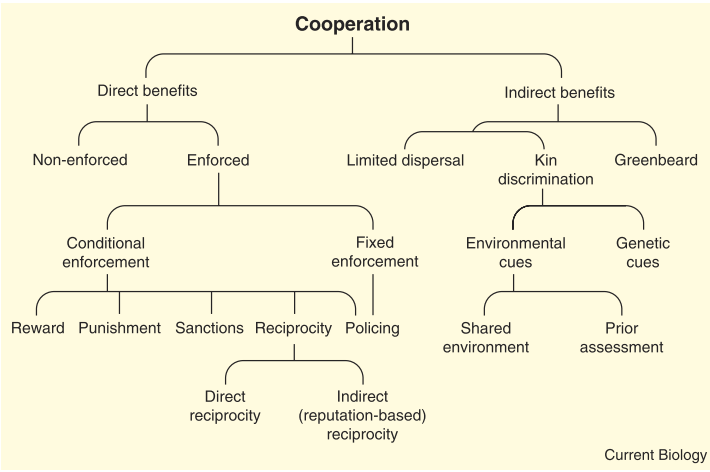
\includegraphics[scale = 0.50]{fig/Intro/ClassificationCooperation.png}
    %       \caption{\textbf{Classification of the mechanisms behind the evolution of cooperation.} Numerous classifications for the explanation of the evolution of cooperative actions have been proposed. However, most people agree that those explanatations can be divided into two categories: direct benefits and indirect benefits. Inside these two main categories, several mechanisms can be invoked in order to understand how cooperation could evolve and be maintained in a population. This picture was taken from the work of West and colleagues~\parencite{West2007}.} 
    %       \label{fig:ClassificationCooperation}
    %     \end{center}
    % \end{figure}

  \subsection{Altruism and Indirect Fitness Benefits}

    A particular type of cooperative actions that has garnered great attention is \emph{altruism}. We consider a behaviour to be altruistic when the actor of the behaviour pays a fitness cost in an action benefitting another individual~\parencite{Hamilton1964, West2007a}. The costly secretion of nutrients by \emph{P. aeruginosas} corresponds, in its simplest form, to an altruistic action. Eusociality is also a major example of altruism in the natural world. In particular, the distribution of reproductive labour means that part of the individuals do not reproduce at all, thus paying the highest fitness cost possible. 

    The main problem posed by the evolution of altruism is its stability against the invasion of cheaters. As previously explained with the example of \emph{P. aeruginosas}, cheaters can easily invade the population and take over cooperators. This sparked numerous research on the evolution of altruism. The now well-known explanation for the evolution of altruism was proposed by Hamilton: \emph{kin selection}~\parencite{Hamilton1964}. This mechanism conveys the idea that a particular trait can spread through the reproduction of relatives. If we consider the unit of selection in evolution to be the gene (as explained by Dawkins with his \emph{Selfish Gene}~\parencite{Dawkins1976}), then the ultimate "goal" of the gene is to spread in the population. It thus does not really matter if a particular individual reproduces or not. If an individual helps another individual that is genetically close to him (i.e. genetically related), he is still transmitting similar genetic material even if he ultimately does not produce offspring. In consequences, an altruistic trait can still spread in the population through helping a relative who may possess this trait: this is kin selection. This general idea of the transmission of one's genes through a relative is encapsulated into the concept of \emph{indirect fitness benefits}. Namely, if a trait contributes to the fitness of relatives, then this trait will also be favoured by natural selection. This wider definition of fitness is called the \emph{inclusive fitness}~\parencite{Grafen1984}, which is constituted of both the direct and indirect fitness benefits.

    % Dire que l'eusocialité s'explique avec kin selection ?

    % The general concept of kin selection is nicely summarized by the popular \emph{Hamilton's rule}~\parencite{Hamilton1964} which states that an altruistic behaviour should be favoured if:

    % \[br > c\]

    % where $b$ and $c$ are respectively the benefits and costs of the cooperative behaviour and $r$ the genetic relatedness between the two individuals (i.e. how genetically similar are the two individuals compared to the rest of the population). To put it more simply, an altruistic trait can be selected if the benefits of this trait weighted by the relatedness to the individuals outweigh the cost of cooperating.

    % While kin selection provides a nice framework for understanding the evolution of altruistic behaviours, it does not provide an explanation on how it is possible to generate sufficient genetic relatedness between individuals for kin selection to function~\parencite{West2007}. Several mechanisms have been proposed to allow kin selection to happen in nature (Figure~\ref{fig:ClassificationCooperation}). The first mechanism is the ability to recognize genetically related partners, also called \emph{kin discrimination}. In particular, kin discrimination can occur through either environmental (e.g. prior associations and living in shared environment) or genetic cues~\parencite{Grafen1990}. For example, long-tailed tits are known to discriminate between kins and non-kins by using vocal cues~\parencite{Russell2001, Sharp2005}. These vocal recognition signals are learned by the adults during the nesting period and the individuals will tend to help primarly individuals with whom they were associated during this nesting period. This causes long-tailed tits to help in the nest of relatives when they have not been able to produce offsprings. Then, and while evidence of its existence are rare, another mechanism is the green beard mechanism~\parencite{Hamilton1964, Lehmann2006}. Rather than focusing on the mean similarity between the individuals' genotypes, this mechanism relates to relatedness on a particular loci in the genotype. The main idea is that a particular gene could be deeply coupled with the "gene for cooperation" and help recognize cooperators at the same time (e.g. thanks to a particular phenotypical trait, hence the analogy to a green beard thanks to which cooperators could be identified~\parencite{Dawkins1976}). Then, cooperators would be more prompt to cooperate with those who express the same trait. However, this sort of mechanisms can easily be used by cheaters who then could profit from cooperators~\parencite{West2007}. A last popular mechanism for the occurence of kin selection is that of limited dispersal~\parencite{Hamilton1972, Griffin2003}. Under limited dispersal, relatives will tend to keep close to one another. What this means is that altruistic cooperation can be directed to any neighbours because those neighbours will tend be strongly related to the individual. Thus, even without any particular discrimination mechanism, it is possible to ensure kin selection.

    Finally, let's quickly touch upon the long time debate about the influence of \emph{group selection} on the evolution of altruism. In particular, the evolution of cooperation was not deemed worthy of studying for some time because it was thought that it could easily be explained by group selection~\parencite{Axelrod1981}. There has been two major branches of this theory, now called old and new group selection theory~\parencite{West2007a}. In the old group selection, it was considered that a cooperative trait could evolve because it was beneficial to the whole group. For example, let's consider that there are two groups in competition, one constituted of cooperators and the other of defectors, who consume resources selfishly. Because defectors exploit their resources selfishly, they would go extinct when resources disappear. Thus the group of cooperators, and therefore cooperation, could survive because selection acted at the level of the group. This is why we may often hear the false idea that an individual will behave in a certain way "for the good of the species". While this particular theory of group selection was then dismissed as nonexistent~\parencite{MaynardSmith1976}, a new group selection theory arised. In this new theory, the main idea is that individuals interact in small groups, which exist inside a given population (whereas old group selection considered the whole population to be the group). Because interactions take place between a small number of individuals inside a given group, then the emergence of cooperative traits can be favored. Since then, it has been shown that kin selection and new group selection are mathematically identical concepts~\parencite{Hamilton1975, VanBaalen1998, Gardner2007} and that it is generally easier to use the kin selection framework~\parencite{West2007a}.


  \subsection{Direct Fitness Benefits and Mutualism}

    % Il faudra avoir parlé de mutualisme avant

    But not all cooperative actions need to be altruistic. In fact cooperation can also be directly beneficial to the actor~\parencite{Leimar2010}. In this case, both the actor and the recipient benefit from the cooperative behaviour and we then say that the behaviour is mutually beneficial~\parencite{West2007a}. Before we talk more thoroughly about this subject we must clarify some confusions that sometimes arise in the litterature~\parencite{Bergmuller2007a}. In particular, some have considered cooperation to only refer to mutually beneficial behaviours~\parencite{Trivers1985, Lehmann2006} in comparison to altruism. Here we consider the broader definition where cooperation includes both altruistic and mutualistic actions~\parencite{West2007a}. There is also some confusion about the definition of \emph{mutualism}. While it can be used to describe mutually beneficial actions or sometimes even cooperation as a whole (as previously explained), it may also refer only to interspecific mutualism. In the context of this thesis, we are mainly interested in intraspecific cooperation. As such, we will tend to follow the advice of West et al.~\parencite{West2007} and use only "mutually beneficial behaviours" rather than mutualism throughout this manuscript.

    % Rajouter les impalas (à la place des primates) sur l'image avec plein d'exemples de coop ?

    Different mechanisms have been proposed in order to explain how cooperation can be adaptive through direct benefits (see Figure~\ref{fig:ClassificationCooperation}. For example benefits can be enforced by the actor in multiple manners. An exhaustive review of enforcement is beyond the scope of this manuscript but we will quickly describe this mechanism to give a general overview of its influence. First, one way those benefits can be enforced is through reciprocal interactions~\parencite{Trivers1971}. Under reciprocity, individuals will tend to help those who have helped them in the past and thus provide mutual (albeit delayed) benefits. In this case, we talk about direct reciprocity. In comparison, under indirect reciprocity an individual will tend to help an individual who is known to help others, hence the notion of "reputation-based reciprocity". It is interesting to note that, outside of humans, reciprocity is thought to be unimportant~\parencite{Dugatkin1997}. However, one well-known example of reciprocity outside humans is in the allogrooming behaviour of impalas~\parencite{Hart1992}. Impalas groom each other in order to remove ticks from the other individual. What is particularly interesting is that grooming occurs in several successive bouts where each individual receive the same number of bouts. This behaviour is widespread and can involve pairs of males, females and fawns. Furthermore, the individuals are unlikely to be related, which removes kin selection as a possible explanation.

    Other forms of enforcement (or coercion~\parencite{Clutton-Brock2002}) include rewards, punishment, sanctions and policing. These types of enforcement are common in humans~\parencite{Fehr2002} but also in a lot of different social animals. Spotted hyenas~\parencite{Drea2003, Drea2009a, Smith2012a} enforce cooperation inside the group through suppressed reproduction. Dominant females will attack lower ranking females if they get pregnant or even their cubs directly. They thus ensure that their offsprings are the only youngs in the group. This way, they enforce cooperative care (alloparenting) of youngs and thus increase their survival chances. Additionally, the cleaner fishes we previously talked about provide a way to distinguish between various enforcement mechanisms. While they eat parasites from their client, their preference would be to eat the mucus and tissue of their client. In return, cliens use different ways to solve this conflict and enforce cooperation (i.e. the cleaner must only eat parasites): partner choice, which means that they go only to "good" cleaners (i.e. cooperators), partner switching, which means they choose to be cleaned by another individual and directly punishing the cleaner through agression~\parencite{Bshary2005}.

    % TODO: Dire que Trivers parlait d'altruistic reciprocity ou on s'en balance ?

    But what we want to study in the context of this thesis is the case where cooperation between individuals is not enforced. Rather, all individuals have a shared interest in cooperating. This is something which is often called \emph{by-product benefits}, conveying the idea that cooperation is a by-product from an otherwise self-interested action. For example, a large group of individuals entails higher chances of survival (against both the environment and predators) and an increase in the benefits from foraging or hunting. This leads individuals to have a mutual benefit in creating groups and societies, something which is known as group augmentation~\parencite{Bergmuller2007a} and has been well studied, for example in the case of meerkats~\parencite{Clutton-Brock2002}. But by-products can also lead to high degrees of coordination between individuals through the benefits of coordinated by-products~\parencite{Leimar2003}. In this case, individuals act in their own interest but also react to the behaviour of others. In particular, cooperative hunting is a very significant type of coordinated by-products. For instance, social carnivores like the spotted hyena display complex coordination strategies in their collective hunting behaviours. In particular, they rely on signaling and communication in order to efficiently coordinate~\parencite{Drea2009a, Smith2010, Smith2012a} and are capable of defending their catch against lions.

    An example of the selfishness involved in by-products was provided by Caraco \& Brown with the Mexican Jay~\parencite{Caraco1986, Dugatkin2002}. When there is food in large enough quantity, these birds will share foods with other individuals' offsprings. While this behaviour may appear altruistic at first, it can be explained by purely selfish motives. In particular, chicks beg loudly until they are fed, which might attract nearby predators. Thus, an individual may share food so that another individual's chicks do not attract the attention of predator to its own offsprings. This example in particular shows that it can be easy to confuse purely selfish behaviours for ones that are altruistics. Similar observations have been made from the behaviours of sentinels, where individuals will take the role of watching for predators in order to alert others from the group. Sentinels might be believed to act in an altruistic manner as they do not forage while they stand guard and might attract the predator's attention to themselves when signaling to others. In the case of the Arabian babbler~\parencite{Wright2001}, an individual goes on sentinel duty only under certain conditions. In particular, individuals will act as watchers when they have already collected enough food to satisfy their need. Being a sentinel is then a way to increase their own survival against predators. Similarly, meerkats selfishly benefit from standing guard~\parencite{CluttonBrock1999}. Additionally, no significant proof that they take a higher risk to be killed by a predator when acting as sentinels.

    Finally, as a conclusion, it is important to state that the differences between all these mechanisms are generally subtle and hard to differentiate. In particular, indirect and direct fitness benefits are not necessarily mutually exclusive and a behaviour can evolved thanks to kin selection but then its benefits can be generated through 
    enforcement.
    

  \subsection{Stability Versus Origin}

    It could be argued that the cooperative behaviours from which all individuals mutually benefit are trivial. In particular in the case altruistic behaviours, the stability of cooperation is under the constant threat of invasion by freeloaders. As such the main problem involved is to study their \emph{stability} against subversion by cheaters. In comparison, when benefits are mutual there does not seem to be any evolutionary puzzle in the same way as with altruism: once a mutualistic behaviour has evolved, there is no incentive to free-ride~\parencite{Forber2015}. While this may be true, this does not take into account the problem of explaining the origin of cooperation~\parencite{West2007}, where it may be difficult for a cooperative behaviour to spread initially. More precisely, focusing on the stability of the cooperative behaviour does not answer the question of how these cooperative behaviours could evolve in the first place, i.e. the \emph{bootstrap of cooperative behaviours}.

    In particular, there is a problem posed by the evolution of mutually beneficial behaviours when they require the evolution of coordination~\parencite{Alvard2001, Alvard2003, Drea2009, Leimar2003}. For example, the evolution of collective hunting is one that is based on interdependence between the individuals~\parencite{Tomasello2012}, which means that the collective success of the group is dependent on the coordination between every individuals. Because of this interdependence, the problem is not one of stability but of shared intention between participants. In consequence there is a fitness valley to cross where all the individual have to evolve coordination before they are able to reap the benefits of collective actions. To put it more simply, we face a \emph{chicken and egg dilemma}. For a cooperative trait to be selected, it needs to benefit the individual. In this case this benefit cannot be obtained unless every individuals coordinate. In consequence, all the individuals must have already evolved cooperation. There has thus been a recent shift in evolutionary biology toward the study of the origin of cooperation (in the case of mutualistic actions) rather than its stability (in the context of altruistic actions)~\parencite{Forber2015}.

    This problem was also defined by Calcott~\parencite{Calcott2007a} as the difference between the \emph{distribution of benefits} (i.e. stability) and the \emph{generation of benefits} (i.e. origin). When we are interested in the distribution of benefits, we focus on the final fitness benefits and costs. That is what we previously did when we tried to explain why altruistic cooperation is adaptive thanks to kin selection (i.e. indirect fitness benefits). But when we focus on the \emph{why}, we tend to abstract from the pratical interactions that take place in order to generate the benefits: we ignore the \emph{how}. The difference between the \emph{why} and the \emph{how} is something that is also known as \emph{ultimate} and \emph{proximate} explanations. This difference was mainly introduced by Niko Tinbergen~\parencite{Tinbergen1963, West2007a} who described the two complementary manners in which we could study animal behaviour:

    \begin{itemize}
      \item {We can study the mechanisms of behaviour to give the proximate explanations}
      \item {We can be interested in the fitness consequences of the behaviour and reveal the ultimate explanations}
    \end{itemize}

    Tinbergen illustrated this difference with the nice example of the black-headed gulls. In particular, these birds remove the eggshells from their nest. The proximate (or mechanistic) explanation is that individuals will more likely remove objects from the nest when they have frilly edges and are egg-coloured and feather-light. The ultimate explanation is that predator are this way less likely to spot their offspring. The conclusion is that both explanations are necessary so that we can fully understand this behaviour. Scott-Phillips and colleagues~\parencite{Scott-Phillips2011} had another way to summarize the difference between these two explanations: proximate mechanisms generate behaviours whereas ultimate functions explain why these behaviours are favored.

    In the case of the evolution of collective hunting, it is thus necessary to study the proximate as well as the ultimate explanations. In particular, because the evolution of coordination is necessary for the emergence of the collective behaviour (and thus cooperation), this means that the mechanistic constraints may have a crucial influence on the ultimate evolution of cooperation. To put it differently, we aim to show that the nature of the coordination behaviours is critical for the capacity to bootstrap cooperation. As previously said, the shift toward explaining the origin of cooperation is pretty recent. As such, few works have focused on the quality of the coordination behaviour (i.e. proximate explanations) which have mostly been considered as a black box~\parencite{Calcott2007a}. We want to show that, by doing as such, critical mechanisms are ignored.

    % TODO: Besoin de faire ressortir plus clairement la problématique ?



\section{Model and Method}

  Now that we have properly introduced the global question asked in this thesis, we are interested in presenting the methods with which our study has been conducted.
  
  \subsection{Game Theory and the Stag Hunt}

    It is classical to use abstract models to study the evolution of cooperation, as we will explain more thoroughly in Chapter~\ref{chapter:model}, where we will provide a more extensive review of models used to that end. Those models are advantageous because they consider general mechanisms and capture the relations between key factors. From purely computational models to spatial simulations, a considerable toolbox of models has been expanded during the past decades in order to increase our understanding of the evolution of cooperation.

    Among all these types of models, the most famous for studying cooperation dilemmas are game theoretical models. The basic idea is that each game represents a particular conflict between several (most often two) players. Each game is provided with a \emph{payoff matrix} whose goal is to indicate for each player, given her strategy and that of the other player, what is her expected reward. This way, the payoff matrix is used to describe the specificity of the game as a whole. Game theoretical models are well used in economy and some of them, like the \emph{Prisoner's Dilemma}, are even highly popular outside the scientific community. As such, evolutionary biologists have also been interest in using game theory as a way to study the evolution of cooperative behaviours. In the case of evolutionary biology, the general framework is called evolutionary game theory~\parencite{MaynardSmith1973}.

    In the context of this thesis, we are interested in a particular type of games: coordination games. In particular, the most well-known representent of coordination games is called the \emph{Stag Hunt}~\parencite{Skyrms2004}. Introduced by Jean-Jacques Rousseau and popularized by Brian Skyrms, this game follows a simple story (see Figure~\ref{fig:MatrixStagHunt})). Two hunters have the choice of either hunting a hare or a stag. Catching a hare is easy for any of the hunters and these prey are present in such availability that we can consider that hunting a hare has no influence on the other hunter's strategy. However, a stag represents a much harder prey to hunt so that both hunters need to cooperate if they want to reap the benefits of going for the stag. Finally, a stag is obviously much more rewarding than a hare. Thus there is a real incentive to cooperate but also a risk of trying to cooperate alone and thus being at a disadvantage compared to the other w.r.t. relative payoff. As for most game theoretical models, the exact payoffs are of no particular interest as long as the order between each situation is respected. In the case of stag hunt, the order for each hunter is as follows: successful cooperation on stag, hunting hare (whatever the partner's strategy) and failed attempt at cooperation.

    \begin{figure}[hbt]
        \begin{center}
          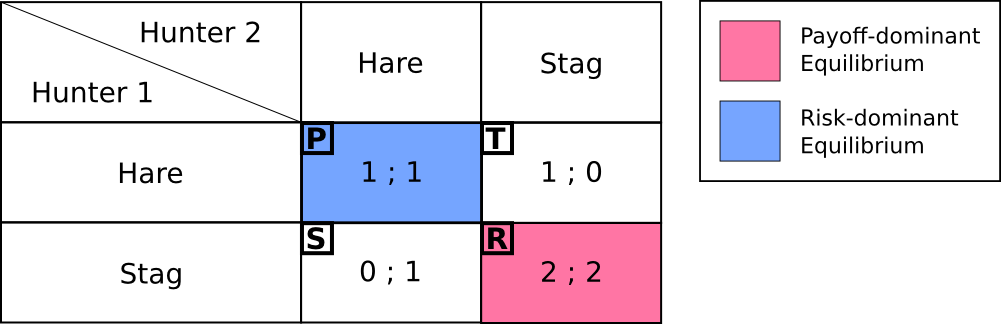
\includegraphics[scale = 0.50]{fig/Intro/StagHunt.png}
          \caption{\textbf{Payoff matrix of the stag hunt.} 
          In the stag hunt~\parencite{Skyrms2004}, we consider that during hunting, two hunters can either hunt a hare or a stag. Hunting a hare can be done in a solitary of cooperative fashion, which ensures that any individual who hunts gets a reward. In comparison, hunting stag can only be achieved in a cooperative fashion but rewards more than a hare. In consequence, an individual who would hunt a stag alone would not get any benefit from hunting. Payoffs are indicated in pair so that we have (Payoff for hunter 1; Payoff for hunter 2). The exact payoffs do not matter as long as the different situations are in that order: R (reward for cooperation) > T (temptation for defection) = P (punishment for defection) > S (sucker's payoff). The payoff-dominant equilibrium is the equilibrium where the hunters maximize their maximum payoff whereas the risk-dominant equilibrium is the one where they maximize their minimum payoff.} 
          \label{fig:MatrixStagHunt}
        \end{center}
    \end{figure}

    The particularity of this game is that there are two evolutionary stable Nash equilibria~\parencite{Nash1950, MaynardSmith1973}. This means that when both individuals hunt hare or when both individuals hunt stag, either strategy is stable against the invasion of mutants. More precisely, this implies that in comparison to the prisoner's dilemma, when the cooperative equilibrium is evolved (hunting stag), its stability is not threatened by the invasion of "defectors" (hare hunters). Thus, in coordination games, cooperation is stable when evolved but risky when rare~\parencite{Forber2015}. Consequently, this game can be used to model the problem of bootstrapping a cooperative strategy.

    But as previously said, when we abstract from the mechanics of behaviours as in game theory we choose to focus on the distribution of benefits at the detriment of the generation of benefits. To put it more simply, when we study the stag hunt we give no explanation on the origin of the coordination mechanisms which allow the individuals to reap the benefits of stag hunting~\parencite{Calcott2007a}. In particular, we tend to assume that the evolution of cooperation is coupled with that of coordination and that evolving cooperation is sufficient to be able to coordinate. In reality, cooperation cannot be beneficial unless coordination is evolved and coordination is not beneficial on its own.

    Our aim during this thesis is thus to model the pratical mechanics of coordination behaviours to study how they influence the ultimate evolution of cooperation. To this end, our approach is that of modeling in \emph{evolutionary robotics}\footnote{The choice of using evolutionary robotics is not without consequences and is not made randomly. In particular, there are critical reasons which justify that we use this technique rather than any other among the numerous modeling frameworks available for evolutionary biology. As this first chapter is a general introduction to this manuscript, we will motivate this choice in Chapter~\ref{chapter:model}}~\parencite{Nolfi2000}.


  \subsection{Evolutionary Robotics}

    Evolutionary robotics (ER) is a method based on designing robots by taking inspiration from natural evolution. In a particular, ER takes the concepts of \emph{selection} and \emph{variation} in order to simply the complex problem of designing a whole robotic systems. The idea of using evolutionary processes in order to solve engineering problems is now new. The whole field of evolutionary computing was created on this idea and still offers promising success in optimization problems where more classical methods fail~\parencite{Holland1975, Goldberg1989, Eiben2003}. Evolutionary robotics use the same principles to take on the complex task of designing part or all of a complete robot: sensors, morphology and control~\parencite{Nolfi2000, Floreano2008, Doncieux2015a}. Please keep in mind that the term "robot" is used loosely here and can refer either to a physical or simulated robot here. This does not impact the general method of evolutionary robotics.

    % TODO: Dire que l'EC c'est cool pour les black box trucs ?

    \begin{figure}[hbt]
        \begin{center}
          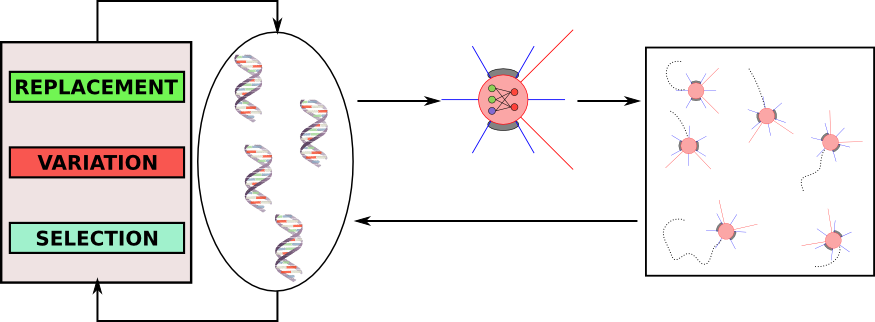
\includegraphics[scale = 0.50]{fig/Intro/EvolutionaryRobotics.png}
          \caption{\textbf{General workflow of an evolutionary robotics algorithm.}
          The main goal of ER is to evolve a population of genotypes. To that end, each genotype must be evaluated to obtain a fitness score. A genotype is thus translated into a phenotype (here an artifical neural network) and then embedded into a robot to act as its controler. The robot is situated in its environment and his behaviour is evaluated in accordance to the specifities of the task. Once every genotype has been asigned a fitness score, they undergo an evolutionary algorithm. This process select the genotypes deemed fit to create offsprings, on which variation is then applied. Finally this new population of genotypes replace the previous population and the process can go on for a new generation.} 
          \label{fig:EvolutionaryRobotics}
        \end{center}
    \end{figure}

    In particular, evolutionary robotics is constituted of an evolutionary algorithm whose goal is to evolve a population of artificial genotypes according to a fitness function (see Figure~\ref{fig:EvolutionaryRobotics}). While the actual format of the genotypes is of no particular interest here, it is but rarely similar to a real genotype in both complexity and features. Most often, each of these genotypes is a randomly generated collection of real values. This genotype is then translated into a phenotype which constitutes the robot's morphology and/or control. Again, the transition from genotype of phenotype as well as the actual phenotype itself can both vary greatly from one model to another. On that matter, one must choose what best fits his needs. The important point is that in ER this is the phenotype which is evaluated. To that end, the robot is situated into its environment and let to interact (with the environment and sometimes other robots). This principle of designing a robot in the context of its environment and the interactions it has with it is known as \emph{embodied intelligence}~\parencite{Pfeifer2007}.
    
    In the more classical models, a fitness function is used to compute the fitness score based on the behaviour of the robot in its environment. For example, in one of the first experiments where an evolutionary process was used to automatically design the control of a robot~\parencite{Floreano1994}, the goal was for a robot to navigate a looping maze. As such, the fitness function that had to be maximized was designed as follows:

    \[
      F = V(1-\sqrt{\delta v})(1-i)
    \]

    where (1) $V$ is the average rotation speed of the wheels, (2) $\delta v$ is the absolute difference between the speeds of the wheels and (3) $i$ the normalized maximum activation value between every sensors (where these sensors were infrared sensors capable of detecting obstacles). Thus, the goal of the robot was to (1) maximize its translational speed, (2) minimize its rotational speed and (3) minimze the activation of its sensors. So, to put it more simply, its goal was to move (1) as fast as possible (2) as straight as possible and (3) by avoiding obstacles at the same time. A large part of designing an evolutionary robotics algorithm is spent carefully crafting the fitness function to evolve the behaviour of the robot according to that desired (which is a challenge on its own).

    It is interesting to note that in those instances of evolutionary algorithm, fitness is thus used to guide the evolutionary process. This is obviously contrary to the biological definition of fitness which is an \emph{a posteriori} observation of the capacity to produce offsprings. While we will but briefly touch upon this subject in our manuscript, it is interesting to know that a few works in evolutionary robotics have been interested in this more "biologically realistic" approach to evolution. In the field of \emph{environment-driven} evolutionary robotics, multiple robots are evolved in open environments where the robotic agents need to encounter other agents so that they can exchange genetic material. Therefore, the selection pressures come from the environment and evolution is driven by the capacity to survive and produce offsprings rather than by a fitness score~\parencite{Ray1991, Bianco2004, Bredeche2010}.

    When every genotypes in the population have been evaluated, a selection scheme is applied based on the fitness score to decide which genotypes will be able to produce offsprings for the next generation. For example, a popular method to select the genotypes is to use \emph{tournament-based} selection. Under this scheme, an offspring results from a tournament between several (from one to the population size) randomly chosen genotypes in the population. These genotypes are then ranked by fitness score and each of the genotypes have a certain probability to be selected. Thus, given a certain probability $p$, the best ranked individual is chosen under probability $p$, then the second best ranked individual under probability $p(p-1)$ and so on. This process is repeated until the desired number of offsprings have been generated. Variation is then finally applied on these offsprings to create the population of the next generation. Variation can consist of mutations and/or crossover. A mutation is the process of randomly chosing one or several genes in the genotype, for example according to an uniform distribution, whose value is then randomly changed (in the way that depends from the format of the genotype). In comparison, the crossover is used to mix the genotypes of two different offsprings. In the most classical way to do crossover, one point crossover, a random point is selected in the genotype and genetic material is swapped between two individuals around this point. Finally, the population of the new generation is created and the evolution process can go on as long as needs be.

    Given the thematic studied in this manuscript, evolutionary robotics is interesting both as a modeling and design tool~\parencite{Trianni2014b, Doncieux2015a}. In particular, because what is evaluated are the phenotypes resulting from the evolved genotypes, this gives the possibility to really observe and study the behaviours evolved. Moreover, as the individual is embodied, we take into account all the interactions between this robot and the environment. This implies that we can study the coordination behaviours evolved in a qualitative fashion. Ecological features and particular mechanisms can then influence the evolution of these behaviours so that their implact on the evolution of cooperation can be thoroughly studied: the mechanics of behaviours are not considered as a black box anymore.



  \subsection{Experimental Setting}

    Now that we have presented both the game theoretical paradigm we take inspiration from and the artificial evolution method, we can finally describe our experimental setting. Please note that, as they may change depending on the exact experiments presented in this manuscript, some of the parameter values are not specified in this section.

    \subsubsection{Robot model} We want to study the evolution of simulated robotic agents (see Figure~\ref{fig:RobotModel}. These agents are capable of movement thanks to two independant wheels and are equiped with a collection of sensors. Those sensors are of two types: $12$ \emph{proximity sensors} and a $90$ degrees front \emph{camera}. On the one hand, the proximity sensors are equally distributed all around the robot's body and inform the agent about the proximity of any obstacle nearby (i.e. in a radius which equals twice of the body's diameter). On the other hand, the camera cannot recognize the obstacles but can feed the agent with the type of any objects it sees in the environment (including other agents). More precisely, this camera is composed of $12$ rays with an infinite range equally divided in the camera's angle. When one of these rays "sees" an object, the agent can know the type of this object and its proximity. The robot is thus constituted of simple sensory capabilities. The choice of having the robot model constituted of two different sensory feedback is not innocent. By dividing the sensory capabilities between the proximity sensors and the camera, we are essentially facilitating the process of evolving two basic capacities necessary for the robot: obstacles avoidance and agents recognition. This design is not to be considered as a realistic approach to evolution but rather as a way to ease the acquisition of basic skills that are of no particular interest here. Furthermore, while the obstacles avoidance mechanism is not expected to improve much during evolution, the appearance of cooperative behaviours in comparison should lead to variation on the manner with which to recognize agents.

    \begin{figure}[hbtp]
        \begin{center}
          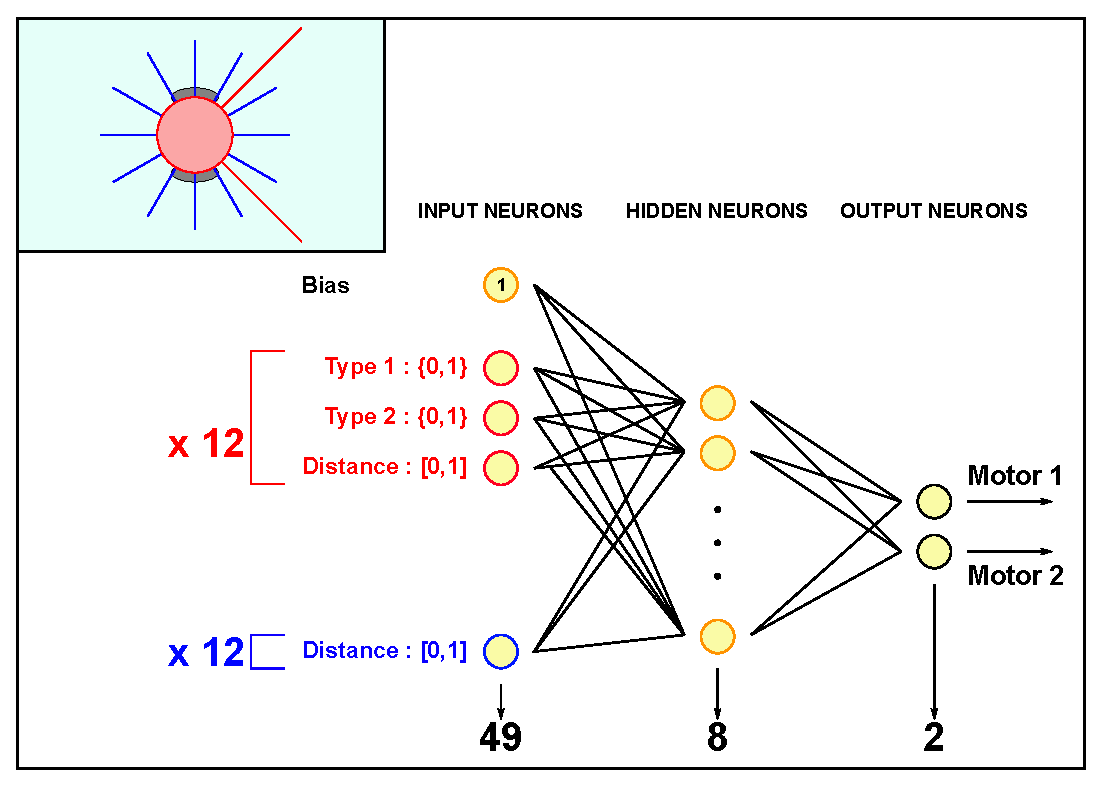
\includegraphics[scale = 0.60]{fig/Intro/RobotModel.eps}
          \caption{\textbf{Robot model of our experimental setting.}
          This figure represents the sensory and neural architecture of simulated robotic agent used in our experimental study. On the robot diagram, proximity sensors are represented by the blue lines whereas the front camera is shown as a red cone. The neural network is a multilayer perceptron with one hidden layer and whose inputs are constituted of all the sensory information of the individual. The outputs of the neural networks are the speeds of both of the robot's wheels.} 
          \label{fig:RobotModel}
        \end{center}
    \end{figure}

    \subsubsection{Controler} The controler of the agent is an artificial neuron network (ANN). While a lot of different types of controlers are used in evolutionary robotics, ANN are widely employed for their versatility~\parencite{Doncieux2015}. The principle behind a very basic neural network is that it is constituted of a layer of input neurons and a layer of output neurons which are connected (sometimes fully) to each other. Each one of the connection has a value, which is called a connection weight. The value of each output neuron is computed as the sum of the input neurons connected to it weighted by the connection weight. A transfer function can then be applied to this output to compute the final value. 

    In our case, we use a fully connected multilayer perceptron with one hidden layer. This neural network is composed of two outputs which are used to compute the speed of each of the robot's wheels. The inputs of the network are constituted of all the sensory information of the robot in addition to a bias neuron whose value is always $1$. This amounts to a total number of $49$ input neurons: $1$ for each proximity sensors, $4$ for each camera ray and $1$ for bias. The information of each camera is encoded by $4$ neurons as we use $2$ bits to encode the type of each object (hare, stag or the other agent) and $1$ last neuron for the proximity of this object. The hidden layer is constituted of $8$ neurons. Finally, the transfer function used in each neuron is a sigmoid and the topology of the ANN is never changed throughout evolution.

    \subsubsection{Environment} We place two evolved robots in an arena with four solid walls. This arena is filled with randomly positioned objects of different type, where the type can be recognized by the camera. These objects represent the prey that can be hunted by the individuals in the stag hunt game. The objects cannot move while the robots can move freely. In order to catch an object, an individual needs to move to this object and then stay next to it for a specified amount of time steps ($800$). After this duration, the object is removed from its position and replaced at another random position in the environment; we thus ensure a constant ratio of each type of object. For cooperation to occur, both robots need to be close to the object at the end of this duration. This thus implies that robots need to display actual coordination behaviours in order to be able to cooperate. This also means that an individual can reap the benefits of cooperation simply by being there at the very last step of the catching period.

    An object is always removed if an individual is next to it after this period of time, regardless of wether it requires cooperation. All that varies are the rewards given to the individuals. Please note that, even in the case of cooperation, we do not study the way rewards are distributed between individuals: they are both equally rewarded.

    \subsubsection{Evolutionary algorithm} The genotypes of the individuals is constituted of all of the connection weights of the neural network. Each gene is initially randomized in the interval where it takes its values, i.e. in \([0,1]\). To evolve these genotypes we use a very classical evolutionary algorithm. At each generation of the algorithm we evaluate each individual of the population in the arena presented before. Its partner is randomly selected in the population. To ensure that each individual encounters a fair sample of the population, each individual is separatly paired with $5$ different partners. Then a pair of individuals interact in the arena during a number of $20000$ time steps. In order to decrease the effect due to the stochasticity in the objects' random positioning, each pair plays $5$ different simulations. Thus, each individual plays a total number of $25$ simulations. Fitness is obtained by computing the average reward of the individual in these simulations.

    The individuals are then selected to produce offsprings. Throughout our experiments, we mainly studied two different selection methods: \emph{fitness proportionate} and \emph{elitist}. The former is the more classical one when modeling evolutionary biology because it corresponds to a Wright-Fisher model~\parencite{Wright1931} with constant population size. Under this model, we randomly sample through the population to select a parent to create each offspring that will constitute the population of the next generation. Each individual in the population has a higher probability to be selected if its fitness is higher. Each individual can also be selected several times. The latter selection scheme is also called a \((\mu + \lambda)\) evolution strategy. With this selection method, we always keep the $\mu$ best individuals of each generation for the next generation. Then we add $\lambda$ offsprings to the population of the next generation, where the parents of these offsprings are taken from the $\mu$ best individuals ranked by fitness score.

    % Justifier Elitist p/r à Fitprop ici ?

    Whatever the selection strategy, we always create the offspring in the same way. Each offspring is a mutated clone of its parent. Then mutation is applied independently on each gene according to the mutation rate. If a gene mutates, mutation is sampled according to a gaussian operator. We thus use no recombination (i.e. crossover) in any of our experiments.


\section{Evolving Coordination in Evolutionary Robotics}

  Until now, we have only introduced the general problem studied in this thesis. Namely, we claim that the proximate explanations of coordination behaviours have a criticial influence on the ultimate evolution of mutually beneficial cooperation. In particular, we believe that the nature of the coordination behaviour is of crucial importance if we want to fully understand the evolution of collective actions. This is what we consider to be the main thematic of the manuscript. 

  However, while this introduction was focused on the biological aspect of cooperation and the problem its origin and stability pose for evolutionary biology, we want to study several facets under this general thematic. In particular, our approach in evolutionary robotics entails that the contributions of this thesis can serve different purposes. Historically, evolutionary robotics has been used at its inception for the automatic design of robotic systems. However, there has been a real problem on how could the works in this field really contribute to scientific research as well as to whom it may be of interest~\parencite{Trianni2014b, Doncieux2015a}. It is now admitted that reseach in evolutionary robotics should be clearly directed toward either of two goals: modeling biological questions or designing robots~\parencite{Trianni2014b}. In this thesis, our goal is to present different contributions which separately aim for each of these goals. We want to quickly introduce each of these goals here to serve also as an introduction to each of the two parts of this manuscript.

  
  \subsection{Modeling the Evolution of Coordination}

    In the first part of this manuscript, we are interested in using evolutionary robotics so that we can model the evolution of cooperation. In particular, as we previously touched upon we want to show that, because we tend to generally ignore or minimize the pratical mechanics of behaviour, the role of coordination in the evolution of collective mutualistic actions is often underestimated. We thus study how the nature of coordination behaviours and the mechanisms that underlie their evolution may influence the ultimate evolution of cooperation. The particular issue we address here could be summarized as follows: \emph{what are the mechanisms which influence the proximate causes of coordination behaviours and facilitate the ultimate bootstrap of mutualistic cooperation ?}

    %TODO: un moyen de faire mieux ressortir la problématique ?

    To that end, we will spend some time in the introduction of this part to really motivate our choice of using evolutionary robotics, something we deliberately skipped in this general introduction. In particular, one reason why the proximate causes of coordination have often been overlooked is that the classical models used for studying evolutionary problems may not be appropriate for this particular goal. We believe that among the distinct assumptions made by these model, some are critical if we plan to fully understand the evolution of coordination. However, it is important to make clear that we do not pretend our approach to be a more realistic depiction of nature. Rather we claim that, while we still study a theoretical abstraction of cooperative actions, the assumptions behind our model allow us to study particular mechanisms we believe of importance for this issue.


  \subsection{Designing Cooperative Robots}

    In the second part of the manuscript, we want to study the evolution of cooperation in a team of heterogeneous robots. In consequence, we focus on the automatic design of a multirobots system. As we will explain more in details in this dedicated part, multirobots systems have now been investigated for a long time for their advantages other single robots. In particular, they may allow to design more efficient and cheaper robotic systems as well as benefit from the redundancy of multiple robots to design more robust systems. Moreoever, it can simply sometimes be necessary to coordinate several robots at the same time to achieve a particular task. The pratical applications of such systems are numerous, in particular in environments where humans cannot go and where using a single and generally more complex robot would simply not be reliable enough. For example, cooperative robots could be used to investigate and perform reparation repairs inside nuclear plants after particularly catastrophic incidents. One could even imagine that it would be useful to send a group of robots to Mars, where robustness is critical and on site repairs are simply not an option.

    However, designing this sort of systems is hard. It is one thing to engineer a factory robot which is programmed to perform a very specific and repetitive task in a controled environment. It is another to design a robot capable of acting in an uncertain environment and able to adapt to the unexpected. And even more complicated when multiple robots must both possess these qualities expected from a single robot and also coordinate in an efficient way. As we will talk about in this part multiple automatic designing techniques have been proposed, in particular for the control of robots. However, when it comes to adaptability to changing environment and uncertainty, the "easiest" way is to design a robot that is capable to learn from previous experiences. In our case, even if considering an evolutionary process to be a particular learning technique is open to debate, we chose evolutionary robotics as a way to design cooperative robots. As for choosing evolutionary robotics to model biological problems, this choice will be dutifully justified in this part of the manuscript. 

    We can however quickly point out that our goal here is to also take inspiration from the results of our modeling of the evolution of coordination. In particular, we are interested in the nature of the coordination behaviours that could be evolved between heterogeneous individuals. Heterogeneous teams of robots allow for more diverse behaviours to emerge inside a group of individuals. However, while there has always been a clear interest on adding heterogeneity in multirobots systems~\parencite{Parker1994, Parker2008}, most research on the evolution of cooperative robots have been focused on homogeneous groups of individuals~\parencite{Waibel2009}. This is indeed one of the safiest way to ensure that robots will indeed evolve a cooperative behaviour, as there is no selfish interest to act in a solitary fashion. However, we believe that the influence of heterogeneity on the quality of the coordination behaviours is as much of importance as the capacity to evolve a cooperation solution. Thus, the issue we focus on in this second part of the manuscript is: \emph{how can we evolve efficient coordination behaviours in a group of heterogeneous cooperative robots ?}


\chapter{Models in Evolutionary Biology and Evolutionary Robotics}
\label{chapter:model}

\epigraph{\textit{So far, we have been able to study only one evolving system and we cannot wait for interstellar flight to provide us with a second. If we want to discover generalizations about evolving systems, we will have to look at artificial ones.}}{--- \textup{John Maynard Smith}}

\setcounter{secnumdepth}{1}
\setcounter{minitocdepth}{2}
\minitoc[n] % minitoc without title

In the first Part of this manuscript, our goal is to model the proximate mechanisms in the evolution of coordination and study their impact on the emergence of cooperation. As in most fields of science, modeling is a standard approach to study questions that cannot be understood by simply observing the physical world. Everything that we now contemplate is the consequence of thousands of millions of years of evolution; the earliest appearance of life is dated back to $4000$ millions years ago and a little more than $2000$ millions for the eukaryotes. This means that we are mostly left with evidence from the past (i.e. paleontological records)~\parencite{Aiello1995, Wrangham1999} or direct observation of evolved behaviours (i.e. ethology). Evolution can also be studied as it is taking place in organisms where it is a much faster process, like microorganisms\footnote{On that subject, a noteworthy experiment is that of Richard Lenski's "Long-Term Evolution Experiment" on Escherichia coli~\parencite{Fox2015}, where he set up in 1988 $12$ populations of the same strain of E. coli and observed their evolution since then.}~\parencite{Elena2003}. However, while empirical works can indeed study the proximate mechanisms of cooperation, they do not inform on the ultimate explanations of behaviours and are not sufficient on their own to garner a full understanding of the process. Thus models are now commonly accepted in the field of evolutionary biology, even if this may not have always been the case~\parencite{Shou2015}. 

As said in the Introduction of this manuscript, we chose evolutionary robotics as our modeling technique for the problem studied. However, we only briefly justified this choice. Thus, the next Sections will be devoted to this task. We will first focus on the different modeling approaches used in the field of evolutionary biology. To that end, we will distinguish between the more classical methods for modeling evolution and the computational methods that arose with the availability of computers. Rather than doing an extensive review of models, we will present the relevance and benefits of these models with regard to our subject. This will finally give us the opportunity to motivate our approach in evolutionary robotics in light of the set of models available and the problem studied in this thesis.


% \section{Why Model the Evolution of Cooperation}

%     While our aim is the modeling of coordination, in this Subsection we are interested in briefly reviewing the more empirical studies of evolution. In this way, our goal is thus to motivate the need to use models in understanding evolutionary phenomona.

%     Everything that we contemplate now is the consequence of thousands of millions years of evolution; the earliest appearance of life is dated to $4000$ millions years ago and a little more than $2000$ millions for the eukaryotes. The time scales involved in the evolutionary process are such that we cannot directly observe evolution but rather to piece together how it could have taken place. This means that we are mostly left with evidences from the past. In consequences, a large part of our empirical understanding comes from paleontologists. A copious amount of work in particular has been dedicated to studying the social life of our hominin ancestors. For example, paleontological records have been used to learn about the diet of early hominins. In particular, those records reveal a strong correlation in our ancestors between the switch to a more energy-rich diet (e.g. meat) and the increase in the brain size of these ancestors~\parencite{Aiello1995, Wrangham1999}.

%     This correlation could hint towards coevolution between the transition to a rich diet and the appearance of social behaviours (which are sometimes argued to require higher brain functions~\parencite{Dunbar2007, Isler2012}). Explanations on how exactly this transition shaped cooperation are diverse~\parencite{Pontzer2012}. Some think that this new diet could allow to adopt more diverse and more efficient hunting and scavenging techniques. Indeed, a richer diet would be necessary to develop the locomotive and cognitive skills necessary for both of these activities~\parencite{Aiello1995, Bramble2004}. Others argue that a shift in climatic conditions led the early hominins to rely more on underground storage organs. While this type of food is rich and available even under arid climate, its harvesting is difficult. This drove selection for the capacity to share food among individuals, thus leading to cooperation~\parencite{OConnell2002}. It is also believed that it led to the emergence of cooking which implied a physical location where individuals would meet and thus create social dynamics~\parencite{Wrangham1999, Wrangham2009}. However, those paleontological evidence do not fare well when trying to understand the proximate mechanisms at play. In particular, it may be difficult to distinguish between the actual causes of the origin of a given evolutionary trait and other phenomena with which its emergence may be correlated. Neither is it easy to come up with general mechanisms for the evolution of cooperation based on these records. For example, the relation between higher brain size and cooperative capabilities (i.e. the social brain hypothesis~\parencite{Dunbar2007}) is now widely debated in evolutionary biology and do not hold under a wider study of social animals~\parencite{Finarelli2009}. 

%     Most of the empirical work on cooperation is achieved by observing animal behaviours (i.e. ethology). In particular, it is argued that it is possible to come with essential explanations of the evolution of sociality in humans by studying that of non-humans. For example, persuasive links have been made between the evolution of cooperation in humans and in social carnivores~\parencite{Schaller1969, Smith2012a}.

%     %, another strong argument in favor of a correlation between the transition to a rich diet comprised of meat and the evolution of social behaviours.

%     As previously stated in the Introduction, most research on the evolution of cooperation have been focused altruism. And as such, a large body of work has been dedicated to finding evidence of kin selection in animals~\parencite{Bourke2014} and in eusocial insects in particular. Only $2\%$ of insect species are eusocial but they represent most of the insects biomass~\parencite{Wilson2008}. In particular, one particularily difficult phenomenon to explain is the presence of reproductive division of labour, where only a certain "caste" of individuals can reproduce~\parencite{Wilson1990}. Empirical works on eusocial insects have shown that colonies are composed of strongly related organisms. In particular, all members of the colony are offsprings of a single individual (i.e. the queen). This validated kin selection as a mechanism to explain the evolution of eusociality~\parencite{Queller1998}. Other empirical works have also investigated the influence of kin selection in vertebrates. In particular, it has been shown that in most cooperative species of birds and mammals, social groups are small and composed of dominant breeders and their relatives~\parencite{Dugatkin1997, Clutton-Brock2002}. In that case, kin selection was brought upon to explain inequalities in breeding between individuals of the same group (something called reproductive skew) and the rearing of youngs by individuals which are not their parents~\parencite{Bourke2011}. However, whereas kin selection is necessary to explain the evolution of altruism in eusociality, the importance of kin selection among vertebrates is much more debated~\parencite{Griffin2003, Clutton-Brock2002}.

%     Field studies on verterbrates have also focused on the role of direct fitness benefits in cooperation. As we previously mentioned, most cooperative actions are likely to generate a combination of both indirect and direct benefits~\parencite{Clutton-Brock2009}. Thus, it may be hard to accurately discriminate cooperative actions that produce direct benefits. However, the presence of intraspecific cooperation between unrelated individuals may only be explained by direct benefits to fitness. For example, spotted hyenas have been shown to cooperate with kin and non-kin alike to achieve collective hunting and defense against other predators~\parencite{Drea2009a, Smith2010, Smith2012a}. Thanks to field work on cooperative vertebrates, various hypothesis on how direct benefits are obtained through social interactions have been proposed~\parencite{Clutton-Brock2002}. For instance, the existence of cooperative breeding can be explained by group augmentation. This means that individuals have a direct benefit in the increase of group size: better protection against predators, more efficient gathering and defense of food and rearing of youngs~\parencite{Packer2001}. More generally, many cooperative actions can be maintained through mutual benefits. Primates are known to engage in mutual grooming and some birds build communal nests which directly benefit every participants. Also collective hunting can profit to every individuals by improving the product of the hunt and decreasing the risk (in terms of both physical risk and missed hunt)~\parencite{Scheel1991}. Cooperation has also been observed to be enforced through coercion, where non-cooperative individuals could suffer punishment or eviction from the group. Reciprocity~\parencite{Trivers1971}, where individuals cooperate with partners with which they previously interacted has often been proposed to explain cooperation between non-kin. However at the moment, there is no sufficient evidence that this type of behaviour occurs in other vertebrates than humans~\parencite{Hammerstein2003, Clutton-Brock2009, Andre2014}.

%     % Mainly good to confirm theoretical hypothesis ?

%     % Je mentionne peu les primates ici. Ca serait bien d'en parler très rapidement (après tout on apprend pas beaucoup de choses vraiment différentes (voir même moins qu'avec les hyènes d'après Drea2009a))

%     It is also worth briefly mentioning empirical studies on cooperation in humans. Human altruism has already been for long studied in economics and it gave rise to experiments that display the existence of altruistic cooperation between non-kins~\parencite{Fehr2002, Fehr2003a}. Altruism in human societies is best explained by a pattern of rewards, reputation and punishment. In particular, they showed the role of strong reciprocity between humans. While altruistic reciprocator will reward and punish individuals if they have a long-term interest~\parencite{Trivers1971}, strong reciprocators will do so in any case (i.e. in a stricly altruistic way). Additionally, some have also been interested in human coordination in mutualistic interactions. For example, Michael Alvard has studied traditional societies of whale hunters in Lamalera, Indonesia~\parencite{Alvard1999, Alvard2003}. In particular, he has shown that there is no significant relation between kinship and the strengh of cooperation in these societies. Alvard thus argues for mutualistic explanations for the evolution of coordinated actions. Moreoever, other studies have also been focused on the mechanisms with which humans coordinate to solve cooperation problems. For example, Bullinger and colleagues~\parencite{Bullinger2011, Duguid2014} have studied how exactly chimpanzees and human childs coordinate in a stag hunt type of game. They have mainly focused on the role of communication and leadership strategies between individuals.

%     % Fehr and Fischbacher~\parencite{Fehr2003a} argue that the evolution of human altruism cannot be only explained by gene-based evolutionary theory alone and advocate for gene-culture coevolution.

%     Lastly, we want to mention the subset of empirical work where cooperation is directly observed while it takes place. This can only done in organism where evolution is a fast process: microorganisms~\parencite{Elena2003}. For example, Richard Lenski conducts his "Long-Term Evolution Experiment" on Escherichia coli~\parencite{Fox2015}. This experiment began in 1988, when Lenski set up $12$ populations of the same strain of E. coli and observed their evolution since then. But more generally, bacteria regularly act in ways that can be caracterized as cooperative~\parencite{West2006}. We previously talked about public goods games in \emph{P. aeruginosas}. But some cells of the slime mould Dictyostelium discoideum have been observed to sacrifice themselves so that other cells can become spores and thus spread their genes~\parencite{Strassmann2000}. Microorganisms have thus often empirically validated kin selection and kin discrimination~\parencite{West2006}. In particular, while green beard mechanisms are thought to be rare, \emph{D. discoideum} are an exemple of this mechanisms. In this case, one gene encodes for individuals to stick to each other to cooperatively form fruiting bodies~\parencite{Queller2003}. But evidence of direct benefits between microorganisms have also been revealed. Mutualism (i.e. interspecific cooperation) is frequent with microorganisms by way of by-product benefits. Evidence of punishing behaviours have also been shown in mutualism between plants and bacteria, like between leguminous plants and the rhizobial bacteria~\parencite{Kiers2003}. In this mutualism, the bacteria fix $N_{2}$ (which is a costly action) that is then supplied to the plant. The plant enforces cooperation by decreasing the supply of $O_{2}$ given to the bacteria should it defect. 

%     %To conclude, it also interesting to note that there are pratical medical applications for studying the evolution of cooperation in microorganisms as there exists a correlation between cooperation and the virulence of bacteria strains~\parencite{Foster2005}.

%     In conclusion, empirical studies on the evolution of cooperation exist and are widespread. However, they rarely inform on the mechanistic constraints involved in the evolution of coordination: proximate explanations are difficult to understand when you can only observe the ultimate results of such a long process. In comparison, in the particular case of microorganisms, microbiologists are concerned with proximate explanations of cooperation~\parencite{West2006}. However, they do not offer the wide variety of coordination behaviours compared to what can be observed in bigger organisms. Moreover, cooperation in microorganisms is based in majority on kin selection mechanisms or interspecific mutualism.

%     % Parler de ce que dit Smith sur protection against predators ?
%     % Man the hunted

%     % Phylogénétique ?

\section{Classical Models in Evolutionary Biology}

    It is nowadays classical in evolutionary biology to use modeling to address the evolution of cooperation (among other evolutionary traits). It is also necessary to do so to fully grasp the mechanisms at play. Models are thus numerous and a lot of different frameworks have been proposed to classify cooperative actions~\parencite{Dugatkin2002, Sachs2004, Lehmann2006}. To that end, mathematical models dominate the field~\parencite{Servedio2014}. 

    \subsection{Population Genetics}

        \emph{Population genetics} form a large part of the literature in evolutionary biology. The inception of this field was mostly the result of Ronald Fisher, J.B.S. Haldane and Sewal Wright. Fisher was the first to link mendelian inheritance (i.e. the inheritance of biological traits) with mathematical models of natural selection in his book \textit{The Genetical Theory of Natural Selection}~\parencite{Fisher1930}. Population genetics is concerned with studying the changes in alleles' frequencies at a particular locus in the genotype. In particular, the focus is put on population wide variations of evolutionary traits within one or a few loci. As such, there has been a strong emphasis on studying genetic mechanisms like dominance, epistasis or genetic drift. A notable branch of this field, \emph{quantitative genetics} have in comparison been more focused on the phenotypical aspects of evolution. More precisely, quantitative genetics deals with continuously varying phenotypical traits. It thus abstracts from the genetic details of evolution. However, population and quantitative genetics both tend to abstract from the role of ecological features which we are interested in here.

        % Because these features are what we are interested in here, we do not focus more on the framework of population genetics.

    % -> Parler de kin selection ici
    % -> Good for ultimate explanations
    % -> Introduire modèles de Moran et Wright-Fisher ? (et probablement équation fondamentale de Fisher. En gros montrer à quel point c'est mathématique ET fondamentale) 

    % Reprendre la partie sur population genetics

    % Dire bien que pop gen ça nous intéresse pas vraiment vu qu'on s'intéresse au phénotype

    \subsection{Evolutionary Game Theory}

        \subsubsection{Matrix games}

            In comparison to population genetics, \emph{evolutionary game theory} (EGT) puts a strong emphasis on ecological aspects. Game theory was originally conceived by the mathematician John von Neumann as a way to determine the optimal strategies in a contest between several (usually two) "players". Given a payoff matrix, each player can expect a certain payoff depending on his strategy and that of other players. In this framework, players are expected to be rational and follow this optimal strategy. One of the most important concepts of game theory is the \emph{Nash equilibrium}~\parencite{Nash1950}. Under a Nash equilibrium, no player benefits in deviating from his strategy if the other players keep their strategy. This framework was first adapted to darwinian evolution by John Maynard Smith and George Price under the name of evolutionary game theory~\parencite{MaynardSmith1973}. The novel idea is that the players' strategies are based on their phenotypes rather than a rational choice. Therefore, an individual's strategy is now inherited and the evolutionary success of the different strategies are studied. To that end, the payoff matrix of an evolutionary game corresponds to the fitness value of each strategy. In order to study the evolutionary dynamics of an evolutionary game, we consider a population of individuals all playing the same strategy. We then assume the appearance of a rare mutant who plays a different strategy and study the fate of these two strategies. If the strategy of the mutant has a higher fitness than that of the initial population (called the \emph{resident strategy}), then it may invade the population and replace the resident strategy. Otherwise, the mutant strategy will not be favoured by selection and will disappear. If this resident strategy is stable against any mutant strategy, we say that this strategy is evolutionarily stable (ESS)~\parencite{MaynardSmith1973}. Interestingly, all ESS are Nash equilibria (but the opposite may not hold).

            One of the main feature of evolutionary game theory in comparison to population genetics is that it takes into account the influence of an individual's behaviour on the fitness of others. More precisely, the fitness of an individual depends on the proportion and behaviours of other individuals in the population, which is known as \emph{frequency-dependent selection}. As such, EGT is convenient in order to account for the ecological features of a particular evolutionary phenomenon~\parencite{Hammerstein1994}. Because it represents conflictual and cooperative interactions, there is a great interest in using EGT for the study of the evolution of social behaviours~\parencite{Bshary2015}. A large body of work in particular has focused on the stability of altruism when faced with the appearance of free-riders (defectors) in the prisoner's dilemma~\parencite{Requejo2013a}. The prisonner's dilemma is a famous game where the only evolutionary stable strategy is for both individuals to defect. Therefore studying how the cooperative equilibrium could be stable in this situation is challenging. Another famous example is that of reciprocity in the \emph{Iterated Prisoner's Dilemma}~\parencite{Axelrod1984}. Axelrod \& Hamilton proposed that individuals play an iterated version of the prisoner's dilemma (of which you can find Axelrod \& Hamilton's payoff matrix in Table~\ref{table:payoffIPD}). To put it more simply, when individuals have engaged in one prisoner's dilemma interaction, there is a probability that they will meet again in a later interaction. They showed that, under those circumstances a particularly efficient strategy was one called \emph{Tit for Tat} (TFT). Under this strategy an individual always cooperates when meeting an opponent for the first time. It then always copies the opponent's last move which means that it (1) retaliates and (2) does not hold grudges. This strategy was thus presented as a theoretical example of reciprocity~\parencite{Trivers1971}.


            \begin{table}[ht]
            \centering
              \begin{tabular}{|l|c|c|}
                \hline
                & \textbf{Cooperation} & \textbf{Defection} \\
                \hline
                \hline
                \textbf{Cooperation} & 3,3 & 0,5 \\
                \hline
                \textbf{Defection} & 5,0 & 1,1 \\
                \hline
              \end{tabular}
              \caption{\textbf{Payoff matrix of the prisoner's dilemma.}
              The strategy of player A (resp. player B) is symbolized by each row (resp. column). The payoff of player A (resp. player B) is shown on the left (resp. right). This is the payoff matrix which was used by Axelrod \& Hamilton in their work on Tit for Tat in the prisoner's dilemma~\parencite{Axelrod1984}.}
            \label{table:payoffIPD}
            \end{table}


            In the case of coordination which we are interested in here, the prisoner's dilemma is not appropriate to model the evolutionary dynamics of cooperation~\parencite{Alvard2002, Skyrms2004}. As such, another type of games more suitable for this question was introduced as coordination games and in particular the stag hunt~\parencite{Skyrms2004, Requejo2013a}. The details of this game have already been covered in the Introduction. The major difference with the prisoner's dilemma is the presence of a second ESS as the cooperative equilibrium (i.e. stag hunting). Thus the emphasis of this game is not on the stability of a population of cooperators against the invasion of free-riders (as the cooperative equilibrium is evolutionarily stable) but on the transition from the solitary equilibrium to the cooperative one. In his book, Skyrms mainly studied the influence of location, signaling and partner choice on the evolution of cooperators~\parencite{Skyrms2004}. However, coordination games like the stag hunt have received relatively little attention, especially in comparison to the prisoner's dilemma~\parencite{Iyer2016}.

        % But the literature on coordination games is much smaller than that on the prisoner's dilemma, several works have ben interested on this subject~\parencite{Santos2006, Pacheco2009, Iyer2016}.

    % -> Mentionner les différents types de jeux ? (coordination games, PD etc... (ya un papier là-dessus))

        \subsubsection{Adaptive dynamics}

            In classical EGT (i.e. matrix games), strategies are discrete and generally constitute a finite list. In comparison, most evolutionary traits take values in a continuous domain. We can for example think about the size, flowering rate or investment and allocation of resources~\parencite{McGill2007}. In order to study the evolutionary dynamics of those traits, a continuous version of EGT rose as \emph{adaptive dynamics} (or continuous-trait game theory). This modeling technique can be seen as a way to combine quantitative genetics, by studying the rate of change of a population's strategy, and EGT, by applying the ecological aspect of frequency-dependent selection~\parencite{Geritz1998, McGill2007}. More precisely, adaptive dynamics extends on the notion of evolutionarily stable strategies from EGT. In particular, the concept of ESS as it exists in EGT lacks precise knowledge about the convergence of a given strategy. Namely, we know that an ESS may not be invaded by any mutant strategy once it has spread in the population. Yet, we do not know if this strategy will eventually become established given the initial conditions. This problem of convergence is represented by \emph{convergence stability}. Convergence stability implies that a strategy, thanks to multiple small evolutionary steps, will be able to fix in the population. Both concepts of evolutionary stability and convergence stability do not always come together~\parencite{Eshel1981, Eshel1983}. Behind convergence stability is the idea that the shape of the fitness landscape changes as the resident strategy changes. From this it stems that it may be impossible to evolve an ESS even when it represents a fitness maximum.

            Several key evolutionary concepts that could not be modeled by classical EGT have been introduced through the framework of adaptive dynamics. One such concept is that of "branching points". These occur when a strategy is convergence stable but not evolutionarily stable~\parencite{Geritz1998}. Namely this strategy acts as an evolutionary attractor from afar but, because the fitness landscape changes as the resident strategy changes, this strategy may be a fitness minimum (and thus not ESS). These are called branching points because two different evolving populations may coexist and evolve separately. Branching points have thus been used to model the evolution of speciation~\parencite{Geritz2004}. 

            %Coevolution has also been widely studied in this field, thanks to the modeling of frequency-dependence. In particular, some have been interested in the competitive coevolution of predators and preys and how branching points influence the apperance of ecological niches in these systems~\parencite{Bowers2003}. Cooperative coevolution (i.e. interspectific mutualism) has also been investigated. More precisely, one of the main questions is the incentive for cheaters to profit from the benefits of mutualistic interactions. Thus some have been interested in studying the stability of mutualism against cheating~\parencite{Ferriere2002, McGill2005}. Finally, it is without surprise that the evolution of altruism represents a fair share of research in adaptive dynamics. Most notably, the ecological modeling in adaptive dynamics (as in game theory in general) has allowed to study how dispersal could be a prominent mechanism to decrease kin competition, thus effectively enabling the evolution of altruism~\parencite{LeGalliard2003, LeGalliard2005}.

        \subsubsection{Proximate mechanisms in evolutionary game theory}

            Models in EGT represent a classic framework for the study of the evolution of cooperation. However, they make assumptions that we deem critical for the evolution of mutualistic cooperation. In matrix games, it is often considered that any given strategy can evolve regardless of the resident strategy. In particular, the phenotype of a given individual is often simply modeled as either a "Cooperator" or a "Defector". As such a single mutation is sufficient to evolve one phenotype or the other. In the context of adaptive dynamics, the issue of converging towards a strategy under particular ecological context (i.e. convergence stability) is well studied. However, convergence is addressed under the assumption that the effects of mutations are small and that convergence can be achieved through a series of small evolutionary steps.

            In both cases, these models make assumptions on the availability of mutations; they are considered not to be limiting and the mapping between the genotype and the phenotype is thus not explicitly modeled. As we already explained, the effect of such assumptions is not equivalent depending on whether we are interested in the stability or the origin of cooperation. If we find a strategy to be an ESS when mutations are not limiting (i.e. any mutant can appear in the population), then this strategy is also an ESS under stronger limitations. In comparison, the evolution of such strategy may vary depending on the effects of mutations. In particular, there needs to be a succession of mutants which are each favored by selection between the different equilibria. In consequence, the availability of mutants may be critical for the origin of cooperative traits. Because mutations affect the proximate mechanisms of behaviours, then the nature of these mechanisms is crucial to the appearance of cooperative mutants. In particular, this may be true when the ability to coordinate is necessary for cooperation to be beneficial. Therefore, we believe that there needs to be complementary models that consider these mechanics of behaviour in the context of the evolution of cooperation. Namely, we are interested in models where the individuals are explicitly modeled and thus where minimal assumptions are made on the mechanistic constraints at play in the mapping from genotype to phenotype.

            % Ca pourrait valoir le coup de mieux expliquer en quoi le mapping c'est en lien avec ce que je viens d'expliquer (pas plus d'une phrase)


% Parler plutôt de Computational Biology ? J'aime bien l'idée de parler de techniques de modélisations particulières qui s'inscrivent finalement dans cette opposition plus générale de Classical VS Computational
\section{Individual-Based Modeling}

    The mathematical models presented before are oftentimes labelled as "classical models"~\parencite{DeAngelis2005, Adami2014} and this is how we will refer to them in this manuscript. This term is not used in a derogatory fashion. Rather, this is a way to discriminate between the mostly mathematical models which have been classical in evolutionary biology and a range of models which were born thanks to an easier access to computational power. This allowed to approach biological questions from a different direction that, some would argue, enables to go beyond what is possible with purely mathematical models~\parencite{Adami2012}. However, the line between classical and computational models can sometimes be not so easy to draw and there is a real scientific interest in trying to get the best of both worlds~\parencite{Wilson1998}. In our case, we are interested in the modeling of individuals so that we can take into account the mechanistic constraints in the evolution of coordination behaviours. To that end, we now present the field of \emph{individual-based models} (IBM)\footnote{The term \emph{agent-based model} can often be found in the literature in lieu of individual-based model. Both names refer to the same framework and are interchangeable. While individual-based models are found more often in biological applications~\parencite{Grimm2005}, no real consensus exists on which term to use. We choose to use the latter throughout this manuscript.}~\parencite{Huston1988}.

    As stated in the name, the goal of an IBM is to model individual-level mechanisms. This is very different from most classical models in ecology where the emphasis is mainly put on population dynamics~\parencite{Grimm2005}. This does not mean that research in IBMs do not deal with population dynamics but rather that these dynamics are studied as a consequence of the interactions between individuals. The main focus of an IBM is to study the collective dynamics emerging from individual-level interactions (whether with other individuals or the environment). And more importantly, the particularity of an IBM is that these individuals, which are the building blocks of the system, are the results of adaptation: collective properties arise from these (sometimes simple) individual behaviours.

    IBMs are mostly used to study biological phenomena for which individual variations, and the assumptions that stem from them, are important. DeAngelis \& Mooij~\parencite{DeAngelis2005} set forth five axes along which IBMs are used to model mechanistic details in the variations between individuals:

    \begin{description}
        \item[Spatial variability] {While classical models sometimes take into account spatial organization, IBMs allow to model local heterogeneity between individuals.}
        \item[Life cycle] {The variability of ontogenetic history can be modeled with finer details by using IBMs than with classical models.}
        \item[Phenotypical variation and plasticity] {The influence of individual experience on behaviours can be taken into account. In particular, IBMs can be more appropriate to model the interactions of multiple different behaviours than classical (game theoretical) models.}
        \item[Learning] {Learning is a consequence of lifetime interactions which are dependent on individual variations.}
        \item[Genetics and evolution] {The computational power of IBMs can help study complex evolutionary genetics.}
    \end{description}

    Thus IBMs have been widely used in behavioural ecology for very diverse applications~\parencite{DeAngelis2005}. For example, spatial variability has been of great interest for the study of group patterns. Most notably, models on the formation of groups of animals, whether swarms of insects, flocks of birds, herds of mammals or schools of fishes~\parencite{Huth1992, Reynolds1992, Gueron1996, Couzin2002} rely heavely on the framework of IBMs. Aggregation behaviours were found to easily arise from simple local (individual-level) sets of rules, leading to complex collective behaviours. More generally, IBMs have been used to model ecological phenomena as diverse as the optimal gap between trees in forests models~\parencite{Botkin1972}, movement patterns in prey-predators interactions~\parencite{Smith1991} or differences in foraging between solitary birds and large flocks~\parencite{Toquenaga1995}.

    % This is a perfect illustration of one of the most basic principle of IBMs: emergence. 

    Interplays between IBM and EGT are numerous. Indeed, both methods can be used to focus on the evolution of phenotypes and rely heavily on the ecological features of the system. This led to a great number of research bringing together these two fields "with ease". In particular, it is now common to take spatial interactions into account (e.g. how individuals are located on a graph or network) when studying the evolution of (mostly altruistic) cooperation~\parencite{Hauert2004}. IBMs also give the possibility to more accurately predict the effects of a finite population size while most models in EGT use infinite population sizes~\parencite{Hauert2009}. Additionally, it is possible to more easily model stochastic or conditional strategies. These ecological features can be modeled with classical game theoretical models but at the cost of increased mathematical complexity~\parencite{Hauert2009}. 

    Moreover, individual-level modeling implies that minimal assumptions are made about the effects of mutations on the evolution of individual behaviours. This makes IBMs an interesting addition to EGT when dealing with the modeling of proximate mechanisms. By putting the emphasis on the individual, it is thus possible to clearly study how individual adaptation can lead to the fixation of evolutionary traits at population level. In consequence, some have used IBMs to study the evolution of cooperation. Olson and colleagues have been interested in the evolution of herds~\parencite{Olson2013a}. More precisely, while collective aggregation benefits the individuals in the group, it is also costly for them (i.e. sharing ressources and increasing the risk of being spotted by predators). Thus there is an evolutionary question on the origin of such collective behaviours. They confirmed that the formation of herds could be explained by Hamilton's theory of the selfish herd (i.e. aggregation emerges because every individual tries to put others between itself and the predator)~\parencite{Hamilton1971}. They also showed that predator confusion through aggregation could explain the evolution of such behaviours~\parencite{Olson2013}. Additionally, they revealed that predator confusion may also lead to the coevolution of morphology (vision system) and behaviour for both predators and prey~\parencite{Olson2016}. Finally they showed that group vigilance could allow the appearance of gregarious foraging behaviours without any kinship relations~\parencite{Olson2014a}. Others have been interested in symbiogenesis, which refers to the creation of a new species through the symbiosis of previously independent species. Watson et al. showed with an IBM that such process could occur without any relatedness between the individuals~\parencite{Watson1992}. Wilder \& Stanley used both an IBM and a classical analytical model to show that altruism could evolve thanks to the creation of ecological niches~\parencite{Wilder2015}. 

    Lastly, some have been interested in the individual-based modeling of biological phenomena thanks to the simulation of digital organisms. In AVIDA~\parencite{Lenski1999}, the organisms are programs that compete for CPU time and evolve in a digital environment and the whole framework can be used to model bacterial evolution. The genome of an individual is composed of a sequence of instructions. With this framework, Goldsby and colleagues~\parencite{Goldsby2012} modeled the evolution of division of labour (or specialization), where individuals specialize between different roles. They showed that the evolution of specialists was more frequent when task-switching costs were high. Additionally, they observed that the individuals were able to used stochastic information, location awareness and messaging in order to specialize. The Aevol platform~\parencite{Knibbe2005, Batut2013} also aims at simulating \emph{in silico} bacterial evolution with digital organisms but with an emphasis on a realistic modeling of genomes. As such it has also been used to model the evolution of cooperation. For instance Fr\'{e}noy et al.~\parencite{Frenoy2013} simulated the evolution of cooperation through the production of public goods (i.e. the costly secretion of nutrients). They investigated the influence of genetic architecture for the maintenance of cooperators in the population. They demonstrated the role of second order selection in the protection of cooperation by the entanglement of the genetic architecture.

        % Citer Tarapore2010 ?

        % Il va falloir caser une réflexion plus générale sur les modèles Alife tels qu'AVIDA et Aevol puisque ce qu'on fait c'est de l'Alife, pas de la modélisation de véritables organismes.
        % Pour ça les modèles sont très divers aussi, par exemple AVIDA et Aevol (sans trop s'appesentir ni sur l'un ni sur l'autre) -> Dire que ya un historique Artificial Life là-dessus : Ou plutôt commencer sur le fait que tu PEUX avoir un côté très artificial life (mais est-ce que c'est vraiment du modeling à ce moment-là ? Oui, débatable)
        %     -> En gros la frontière est compliquée
        % Il y a quand même une différence entre de l'IBM pour modéliser des vrais animaux et de l'IBM Artificial Life (donc en gros un peu ce que dit Webb). Va falloir l'expliquer ça à un moment.
        % IBM are diverse ? (genre AVIDA c'est IBM, AEVOL aussi)
        % -> Sometimes closer to reality -> aevol, sometimes further -> AVIDA
        % Si besoin, dans Floreano2010 ya un peu de biblio sur AVIDA (ça sera bien suffisant !)
        % Digital genetics: unravelling the genetic basis of evolution (à garder de côté pour Avida et ALIFE)
        % The ecology of action selection: insights from artificial life Anil K. Seth Pareil (pour ALIFE, pas AVIDA)


% Here we focus on a particular type of IBMs 
\section{Evolutionary Robotics}     

    \subsection{Individual-Based Modeling and Evolutionary Robotics}

        In this thesis, we focus on a particular type of individual-based models: \emph{evolutionary robotics} (ER)~\parencite{Nolfi2000, Doncieux2015a}. The technical details of this framework have already been covered in the Introduction of the manuscript. As such we want to present in this Section the reasons for which one could use evolutionary robotics above (or in addition to) any other modeling techniques presented before. Why should evolutionary biologists be interested in using ER ? And why should we use ER in the context of this thesis ?

        % The reasons are in fact very similar to those in favor of IBMs. Individual-based modeling and evolutionary robotics have actually very comparable features that makes them appealing as a framework. Namely, they both model phenomena at the level of the individual in a particular ecological context and put a strong emphasis on the evolution of phenotypical traits. As in IBMs, ER can be used to model spatial organization and local interactions, life cycle dynamics and any kind of phenotypical plasticity~\parencite{Mitri2013}. ER is thus also appropriate in the study of behavioural mechanisms and their impact on evolution. Therefore, the line between ER and IBMs can sometimes be blurry. It can even be argued that some studies conducted in ER could have led to similar conclusions with a "simpler" IBM~\parencite{Mitri2013}.


        % To summarize quickly what we said in the Introduction, behind evolutionary robotics is the idea of using the Darwinian principles of selection and variation to evolve a robot's controler and/or morphology~\parencite{Floreano2010, Doncieux2014}. At its core, evolutionary robotics is thus a design technique which stems from the need to bring an holistic approach to the conception of a robot. Because creating a fully embodied agent is complex, the key principle is to let evolution do the work. So why should evolutionary biologists be interested in using ER ?

        % Caser peut-être ici le paragraphe de l'intro sur l'embodied (quand on cite Mitri2013) ? En gros pour dire que c'est de l'embodied même si c'est du simulé

        % But that does not mean that there is no profound differences that may motivate the use of ER over IBMs. The main difference between these two frameworks is summarized by the following assertion: 

        The main addition of ER when compared to more general IBMs is that ER models are IBMs where the individual is an embodied agent~\parencite{Mitri2013}. By definition, robots have a body (physical or simulated). In consequence, this creates an additional level of interactions with the environment. Sensory feedback is also part of a robot's design, which means that there often is imperfect information about the environment. In comparison, IBMs will usually (but not necessarily) provide a global and perfect description of the world. Finally, modeling in ER implies that the environment (whether simulated or not) exists in a bounded space, which again may not be the case in IBMs. All of this can have lasting consequences on the dynamics of a system. When those physical properties are expected to be of importance for the phenomenon studied, it may be beneficial to use ER rather than IBMs. Mitri and colleagues~\parencite{Mitri2009} provided an elegant example of a case where physical embodiement led to unexpected results. While their study was focused on the evolution of communication between simulated robots for foraging, they found that the aggregation of robots on a foraging site provided additional information that did not require the use of direct communication. More generally, the line between IBMs and ER in the literature can be blurry. Oftentimes, the differences between both frameworks mainly rest upon terminology and history. Namely, these two techniques come from (at least originally) different communities. ER is deeply rooted in the field of robotics design. In comparison, a large part of the works in IBM is interested in the design of more general multi-agent systems and their applications. While ER and IBM can be very similar, these historical divergences tend to have a lasting effect. Yet, we can simply consider ER models to be a particular instance of IBM as we do here. As such, ER is endowed with similar advantages w.r.t. modeling proximate mechanisms in the evolution of behaviours as IBM.

        There has been an extensive, though recent, effort in using ER as a modeling tool for social behaviours as well as evolution~\parencite{Mitri2013, Trianni2014b, Eiben2014, Doncieux2015a}. However there still is a lack of communication between communities which implies that ER research sometimes fail to reach those who could be interested by these findings in the evolutionary biology community. This also means that some works in ER may sometimes focus on questions that are of no particular relevance for evolutionary biologists~\parencite{Trianni2014b, Doncieux2015a}. We now present some of the more significant works in ER that have been interested in modeling the evolution of social behaviours. 

        First, the evolution of communication has been a major subject of interest in ER. The modeling of individual-level interactions is adamant in understanding the evolution of communication. Additionally, the embodiement of individuals in space can have some unexpected effects on communication behaviours~\parencite{Mitri2009}. Floreano \& colleagues~\parencite{Floreano2007} showed how the evolution of communication could vary depending on the relatedness inside a group of foraging robots. Robots had to correctly choose between a food site and a poison site, where the difference between both sites could only be determined at close range. Communication could easily evolve when there was strong relatedness (i.e. robots were clones of each other). In comparison, when individuals were unrelated, deceptive strategies would also evolve. In a similar setting Mitri et al.~\parencite{Mitri2011} revealed a strong correlation between signal reliability and relatedness between individuals. Related individuals would produce more reliable signals in order to direct others towards the food source. Wischmann, Floreano and Keller~\parencite{Wischmann2012} conducted a study where they observed that purely historical contingencies could lead to divergences in the communication strategies evolved in independent evolutionary runs. In particular they showed that signaling strategies of varying complexity could evolve based on these contingencies. The more complex strategy would not ensure higher performance unless in a competitive setting between different populations (a setting in which populations were not evolved). Finally, Mitri and colleagues~\parencite{Mitri2009} focused on the evolution of both communication and suppression of signaling in a competitive environment. They observed suprising evolutionary dynamics. While robots were quickly selected not to emit light on the food source (because it helped competitors find the food source), signaling was never completely suppressed. They found that it could be explained by the fact that the strength of selection for suppression decreased as the information in the signal diminished. Others have been interested in the evolution of swarming behaviours. As said earlier Olson \& colleagues have studied the evolutionary mechanisms behind the emergence of herding behaviours~\parencite{Olson2013, Olson2013a, Haley2014}. While they categorize their work solely as IBM, it could be argued that their study belongs more precisely to the field of ER as they model evolution between embodied agents.

        In consequence, evolutionary robotics allows to model individual variations and thus study their influence on the evolution of a given evolutionary trait. This implies that we can model the mapping from genotype to phenotype without making critical assumptions about the mechanistic constraints at play. Additionally, in comparison to IBM the embodiement that comes with ER decreases the assumptions we make on the exact nature of behaviours. This means that it may be possible for evolution to find unexpected solutions to coordinate which may not require any particular sensory or communication capabilities. This is appropriate as we do no want to limit the diversity of the possible behaviours which could evolve.

         % This is why we believe ER to be a fitting framework for the problem studied in this thesis.

        %  This is another evidence of the interplay between the two communities. Quite differently, Elfwing \& Doya~\parencite{Elfwing2014a} have been interested in the evolution of polymorphism, where individuals with different phenotypes coexist in the same population at the same time. More precisely, they simulated an environment filled with energy sources that an individual needs to collect to ensure its survival. Moreover, the individuals had to physically exchange genotypes with other individuals in order to simulate mating and produce offsprings. The individuals could choose between two different strategies, focusing (1) on the energy sources or (2) on tracking mating partners. They observed the evolution of polymorphic evolutionary stable strategies. 

    \subsection{The Evolution of Cooperation in Evolutionary Robotics}

        % As previously said, several works have been interested in the modeling of evolutionary biology questions with tools from evolutionary robotics. But some in particular have focused on the evolution of cooperation. As a final Section for this Chapter, we review the works on this subject as to show where we stand in the context of this literature.

        % Again, as cooperation is one of the major puzzle in evolution, a portion of the studies that model evolution in ER has been interested more directly on the emergence of cooperation. 
        As a final Section for this Chapter we review the works in ER that have been interested in the evolution of cooperation to present where we stand in this context. As is common when studying the evolution of cooperation, most works have been focused on altruism. Waibel \& colleagues~\parencite{Waibel2011} conducted an empirical test of Hamilton's rule\footnote{Hamilton's rule is a way to summarize the effect of kin selection by stating that an altruistic trait may be selected if the following inequation is respected: $rb > c$, where $b$ and $c$ are respectively the fitness benefits on the recipient and costs on the actor of the cooperative interaction and $r$ is the relatedness between the recipient and the actor. In consequence, an altruistic behaviour is favoured when the benefits of this behaviour weighted by the relatedness with the actor outweigh the cost of cooperating.}~\parencite{Hamilton1964} for the evolution of altruism in a group of robots. They designed a foraging task where robots had the possibility to share with others their benefits obtained from foraging. They then tested how the coefficient of relatedness between robots influenced the evolution of altruism (i.e. sharing foraged ressources). They showed that, in this context, Hamilton's rule is indeed quantitatively validated. Similarly in another study they have been interested in the influence of both the genetic composition of groups of robots (homogeneous or heterogeneous) and the level of selection (individual-level or group-level) in the evolution of cooperation~\parencite{Waibel2009}. In particular, they studied the impact of these two criteria on the performance of robots in three different foraging tasks: a solitary one, a cooperative one and an altruistic one. As could be expected, teams where individuals were homogeneous (i.e. where genetic relatedness was equal to $1$) performed better in tasks which required cooperation. Montanier and Bredeche have also studied the evolution of altruism in an \emph{environment-driven} model. In this type of models, selection pressure comes solely from the environment. As such no fitness function is explicitly defined and individuals need to meet each other so that they can exchange genetic material~\parencite{Bredeche2010}, which is a more "realistic" approach to modeling evolution. In particular, they studied the evolution of altruism in a foraging setting under a "tragedy of commons" situation~\parencite{Hardin1968, Montanier2011}. This means that individuals have to share a common limited ressource to such extent that some individuals may have to die so that the whole population does not go extinct. They showed that altruism can evolve under sufficient genetic relatedness. In another similar study~\parencite{Montanier2013}, these authors validated the existence of a negative correlation between the evolution of altruism and spatial dispersion. More precisely, under low dispersion individuals tend to interact with other nearby individuals. Thus they interact with individuals that are more genetically related to them, which generates sufficient genetic relatedness so that kin selection can occur~\parencite{VanBaalen1998}. 

        Others have been interested in the evolution of division of labour. These studies have in particular focused on the evolution of specialization in ants. Ferrante et al.~\parencite{Ferrante2015} proposed an ER model of task-partitioning (where a task has to be done in sequence) in leafcutter ants. In this species, some ants are tasked with cutting leaves and leave them in a storage location from which other ants collect the leaves and bring them back to the nest. They showed that division of labour could evolve when particular environmental features (in their case a slope) could be exploited to reduce switching costs. They thus validated a biological hypothesis about the role of switching costs in the evolution of specialization~\parencite{Duarte2011}. 

        % Tarapore ? -> Bof c'est VRAIMENT pas de l'ER

        Solomon and colleagues~\parencite{Solomon2012} are among the few who have been interested in modeling the evolution of cooperation between unrelated individuals, i.e. where cooperation is necessarily mutually beneficial (as altruism cannot evolve between unrelated individuals). They studied the evolution of signaling strategies in cooperative robots. In particular, they took inspiration from the hunting behaviours of spotted hyenas~\parencite{Smith2012a} in the context of competition against lions for the stealing of a prey. They compared the performance of two different signaling strategies: (1) one where all individuals can signal to the others and (2) another one where only a particular individual, the flag-bearer, may signal. The latter strategy was revealed to achieve higher coordination between individuals and therefore to increase the benefits of the cooperative action.


\section{Conclusions}

    In conclusion of this Chapter, we do not claim any model to be fundamentally better than the others. As we previously stated in the general Introduction each model is based on assumptions and a specific level of abstraction. The choice of a model is made depending on which assumptions we expect to be of critical importance. Even considering a particular model to be globally more realistic can be tricky; some models simply represent more accurately a particular aspect of a phenomenon. Mitri and colleagues~\parencite{Mitri2013} classified models for the study of social behaviours according to their situatedness, which they defined as "the extent to which individuals are embedded in an environment that they can sense and modify". In this Chapter, our goal was to show that classical models in evolutionary biology make assumptions on the availability of mutations that we consider to be of importance in the evolution of mutualistic cooperation. In particular, we claim that the appearance of mutants (and thus the emergence of cooperation) depends on the proximate mechanisms of coordination. We thus motivated our choice of using individual-based modeling to address this issue. Thus we can model the mapping between genotype and phenotype and thus study the influence of mechanistic constraints on the evolution of cooperation. The framework of evolutionary robotics is relevant as we make no assumption on the nature of the behaviours evolved, which may allow for a higher diversity of coordination strategies.
    % TODO: (see Figure TODO -> La refaire moi-même en mettant ce qui m'intéresse plus précisément).

    In the next two Chapters, we will thus be interested in using ER to study the impact of the mechanics of coordination behaviours on the evolution of cooperation. First, we focus on comparing the evolution of collective hunting in a classical game theoretical model and in evolutionary robotics. We study the differences between these two approaches with regard to the emergence of a cooperative strategy. We thus investigate the role of coordination in the transition to cooperation. Then, in a second Chapter, we study more precisely how the nature of coordination strategies influence the evolution of collective actions. Namely, we are interested in the transition from a suboptimal collective equilibrium to the optimal one. We want to study how the evolution of different coordination strategies may impact the emergence of such transition thanks to individual selection only. In both of these studies, no physical robots are used. While it could allow to endow our studies with real physics (e.g. friction), we do not believe that level of realism to be of critical importance in this context. As with any model, we choose to abstract from some aspects of the real world that we think do not impact our results. Moreover, experiments on physical robots are in any case unfortunately too time-consuming to consider using them to such scope~\parencite{Mitri2013, Doncieux2015a}.

    % In the case of the problem studied in this chapter, we need a framework which can model the mechanistic constraints in the evolution of coordination. We previously showed that EGT has been widely used in the context of coordination games, which explains why we take inspiration from the stag hunt. However, as we touched upon in the Introduction, models in EGT tend to make critical assumptions on the availability of mutations. Namely, it is often considered that any given strategy can evolve regardless of the resident strategy. Thus, the problem of convergence, which we expect to be of utmost importance here, is usually ignored. In comparison, we claim that the mutational steps necessary to boostrap cooperation are dependent on the proximate mechanisms of coordination. In adaptive dynamics, this problem is addressed through the concept of convergence stability. In particular, the variations in resident strategies affects the fitness landscape which may hinder the convergence of particular strategies. However, other assumptions are once more made: that the effects of mutations are small. We want to show here that the mechanistics constraints in the evolution of coordination behaviours may prevent the evolution of collective actions. Thus we aim to use a framework where no particular assumptions are made on the effect of mutations in the evolution of coordination strategies.

    % Là faudrait caser un jour une réflexion sur l'abstraction de notre modèle et l'approche animat. En gros répondre à Webb.


% \section{To Cooperate or not to Cooperate: why Behavioural Mechanisms Matter}
  \subsection{Introduction}
    It is well known that, in the absence of genetic relatedness, altruistic behaviours in which individuals pay a fitness cost for the benefit of others cannot evolve by natural selection \parencite{Hamilton1964,West2007a}. However, it is often assumed that mutualistic behaviours, wherein individuals collectively gain a common benefit~\parencite{Leimar2003, Leimar2010}, do not pose such a problem, and are therefore of limited interest to evolutionists: they simply evolve because they benefit the individuals who express them.

    However, mutualistic behaviours do often pose a different kind of evolutionary problem than altruism: they require coordination \parencite{Alvard1999, Alvard2003, Drea2009, Leimar2003}. Many collective traits are only mutually beneficial if several individuals express them together in a coordinated fashion. That is, it would not be beneficial for a single individual to express the cooperative trait if others did not express it as well. Consequently, whereas altruistic behaviours pose a problem of \textit{stability}, which can only be solved by genetic relatedness, many forms of mutualistic behaviours pose a problem of \textit{evolution}. These collective strategies are stable equilibria but their evolution is complex. 

    This problem has been formalized in game theory as the stag hunt game \parencite{Skyrms2004}. In the stag hunt, two hunters are confronted with the choice of either hunting a hare alone for a small but guaranteed benefit, or coordinating to hunt a stag cooperatively for a bigger reward, with the risk of not being rewarded at all if they hunt the stag alone. There are two evolutionarily stable Nash equilibria in this game: (1) simultaneous defection (i.e. both players hunt hares), which is risk-dominant as it maximizes the minimum payoff an individual can expect, and (2) simultaneous cooperation (i.e. both players hunt stags), which is payoff-dominant as it maximizes the total payoff at equilibrium. One of the aims of evolutionary analyses of the stag hunt is to characterize the mechanisms that facilitate the transition from the solitary equilibrium to the cooperative equilibrium. The difficulty is that cooperation can only be favoured by selection when a sufficient proportion of individuals in the population also cooperate. The transition from a population with a majority of solitary individuals to one with a majority of social individuals requires the rise of cooperation above an invasion threshold, which must occur for non-selective reasons.

    In game-theoretic analyses, the hunting strategy of individuals is generally assumed to be encoded by a single genetic locus with two alleles: solitary or social~\parencite{Skyrms2004}. In this case, random mutations and/or demographic stochasticity can lead to the appearance of a subpopulation of mutants playing the social strategy which is sufficient to overcome the invasion threshold. Moreover, Skyrms~\parencite{Skyrms2004} showed that this cooperation can be further facilitated in a spatially structured population in which individuals tend to interact more with genetically related partners. 

    However, this approach makes a very strong assumption about the underlying mechanistic nature of behaviour: that a single mutation is sufficient to transform an individual playing a solitary strategy into an individual playing a perfectly efficient social strategy. In reality, hunting socially implies several novel behavioural abilities. In particular, it implies the ability to coordinate with others in order to focus on the same prey, which is unlikely to occur with only a single random mutation. In this paper, we postulate that critical aspects of coordinated cooperation have been neglected by game-theoretic analyses and investigate the mechanistic constraints which interfere with the evolution of coordination in a more realistic setting where the mapping between genotype and phenotype is not limited to a strict binary encoding. 

    Evolutionary robotics is a useful methodology for the simulation and study of this more realistic conception of behaviour and its genetic underpinnings\parencite{Nolfi2004, Doncieux2015}. This approach allows to simulate the evolution of complex genotypes and observe the resulting behaviours in robotic agents. Such simulations also make it possible to investigate the complex mechanistic constraints at play in the translation from genotype to phenotype~\parencite{Mitri2012}. A considerable body of work has already been dedicated to modeling social evolution with robotic approaches~\parencite{Trianni2014}. These studies have been interested in a large diversity of issues: the evolution of swarms~\parencite{Olson2013}, the mechanics of division of labour in social insects~\parencite{Tarapore2010, Ferrante2015} or the evolution of communication~\parencite{Floreano2007, Mitri2011, Wischmann2012, Solomon2012}. The evolution of cooperation in particular has been addressed in numerous papers. In the vast majority of this literature, however, social partners are genetically related~\parencite{Waibel2009}, whether motivated by design~\parencite{Hauert2010, Trianni2007} or to study the evolution of altruism~\parencite{Waibel2011, Montanier2013}. Few articles, in comparison, have been interested in the evolution of mutualistic cooperation between genetically unrelated individuals~\parencite{Solomon2012}. Moreover the specific problem posed by the stag hunt game, where cooperation is not the only evolutionarily stable strategy and a non-collective solution acts as a stable attractor, has never been studied in evolutionary robotics.

    In this paper, we use an experimental model where simulated robotic agents interact in a situation equivalent to the stag hunt and compare the results of our model to those of standard game-theoretic analyses. Our results shed new light on the influence of mechanistic constraints in the evolution of coordinated actions. We then use this model to explore realistic mechanisms that could drive the transition to collective behaviours.

  % You may title this section "Methods" or "Models". 
  % "Models" is not a valid title for PLoS ONE authors. However, PLoS ONE
  % authors may use "Analysis" 
  \subsection{Materials and Methods}
  \label{sec:methods}
    \subsubsection{Experimental Setup}
    \label{setup}
      We consider an environment with two hunters and several prey, both hares and stags. Hunters can choose to hunt either of these prey, earning different food rewards depending on whether they hunt alone or cooperate (see Fig.~\ref{fig:figureSimulation}).

      \begin{figure}[hbtp]
        \centering
          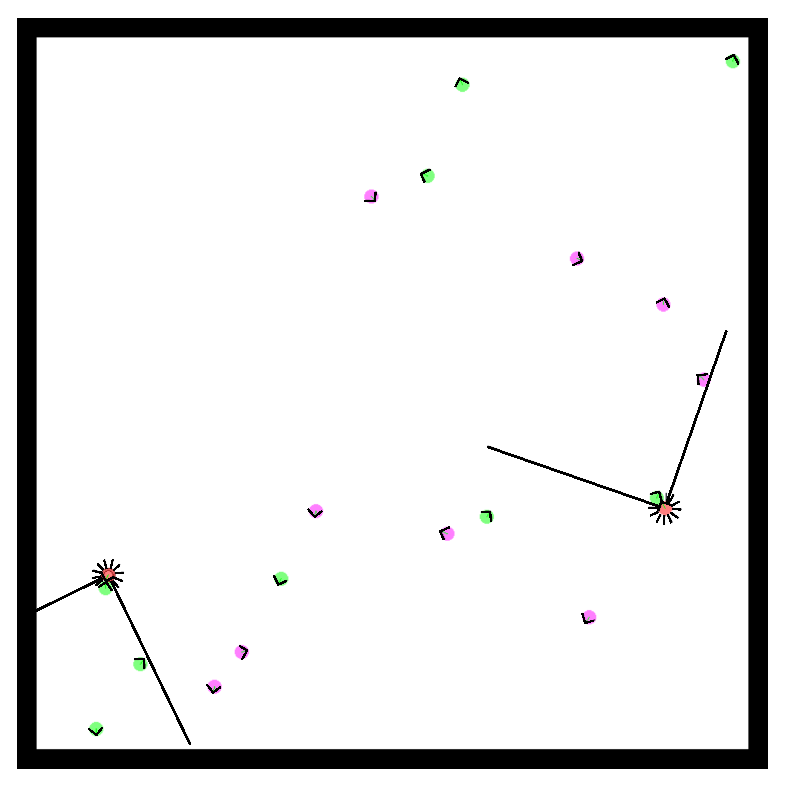
\includegraphics[scale = 0.25]{fig/ArticleBio1/Fig1.eps}
        \caption{\textbf{Screenshot of a robotic simulation.} 
        The red dots represent the two hunters, the green dots the hares, and the pink dots the stags. The black lines around the agents' body represent the proximity sensors and the black cones on front the cameras described in the text. Hunters are allowed to move throughout the environment. Hares and stags remain at their starting positions.}
        \label{fig:figureSimulation}
      \end{figure}

      Food rewards for killing a prey are shown in Table~\ref{table:tableRewardsInitial}. A hare yields a reward of 50, regardless of whether it is hunted in a solitary or cooperative fashion. A stag yields a reward of 500 for each hunter only if it is hunted cooperatively. If a stag is killed by a single hunter, it is still removed from the arena but is considered a failed hunt and rewards nothing. None of the rewards are split between cooperators.

      \begin{table}[ht]
        \centering
          \caption{\textbf{Food rewards for hunting different prey.}}
          \begin{tabular}{|l|r|c|}
            \hline
            \multicolumn{2}{|l|}{\textbf{Prey}} & \textbf{Food Reward} \\
            \hline
            Hare & \textit{alone} & 50 \\
            \hline
            & \textit{coop.} & 50 \\
            \hline
            Stag & \textit{alone} & 0 \\
            \hline
            & \textit{coop.} & 500 \\
            \hline
          \end{tabular}
          \begin{flushleft} The reward depends on whether these prey were hunted alone or cooperatively. There is no reward for stags hunted alone in this case.
          \end{flushleft}
        \label{table:tableRewardsInitial}
      \end{table}

      Simulated robotic agents are evaluated in an 800 by 800 unit square arena, which has four solid walls and is devoid of any obstacles aside from other agents. Each circular-shaped agent, with a diameter of 14 units, is equipped with two independent wheels and a collection of sensors. Hunters can use the information provided by 12 proximity sensors and a front camera. Proximity sensors have a range of approximately twice the diameter of the agent's body, and provide the agent with the proximity of the nearest obstacle. They are evenly distributed around the agent's body. The front camera consists of 12 rays with infinite range spread out in a 90 degree cone in front of the body. Each ray in the camera provides two different pieces of information about the first target it intersects with: the type of target (hunter, hare, or stag) and its proximity. This robot model facilitates the evolution of basic walls avoidance and agents recognition behaviours, which we consider not to be of interest here. Hence we separate obstacles recognition (by the proximity sensors) from agents' recognition (by the camera).

      Only the hunters are capable of movement; prey remain at their initial positions. (Complementary experiments with moving prey capable of avoidance behaviours did not produce significantly different results; not shown.) A prey is caught if any hunter remains close enough during a fixed amount of time steps (800 steps, in a simulation lasting 20.000 time steps). Cooperative hunting is defined as a prey with two hunters in catching distance at the time of its capture. Therefore, cooperation happens even if only one of the two hunters is in catching distance of the prey for most of the time, as long as the two hunters are there in the final step. The prey is then immediately replaced at a random position in the arena, thus keeping a fixed number of agents and prey during the whole simulation.


    \subsubsection{Neural Network for Agent Control}
    \label{nn}
      The hunters' behaviour is computed by an artificial neural network which maps sensory inputs to motor outputs. The neural network is a fully connected multi-layer perceptron with a single hidden layer of 8 neurons. The inputs of this network are the perceptions of the agent, with 12 neurons for the proximity sensors and 48 for the camera (4 for each of the 12 rays) plus a bias neuron (whose value is always 1), for a total of 61 input neurons. The two outputs of the network control the speed of each of the agent's wheels and the mapping function between inputs and outputs is a sigmoid function (see Fig.~\ref{fig:robotDescription}). Changing the number of hidden neurons did not yield significantly different results (not shown).

      \begin{figure}[hbtp]
        \centering
          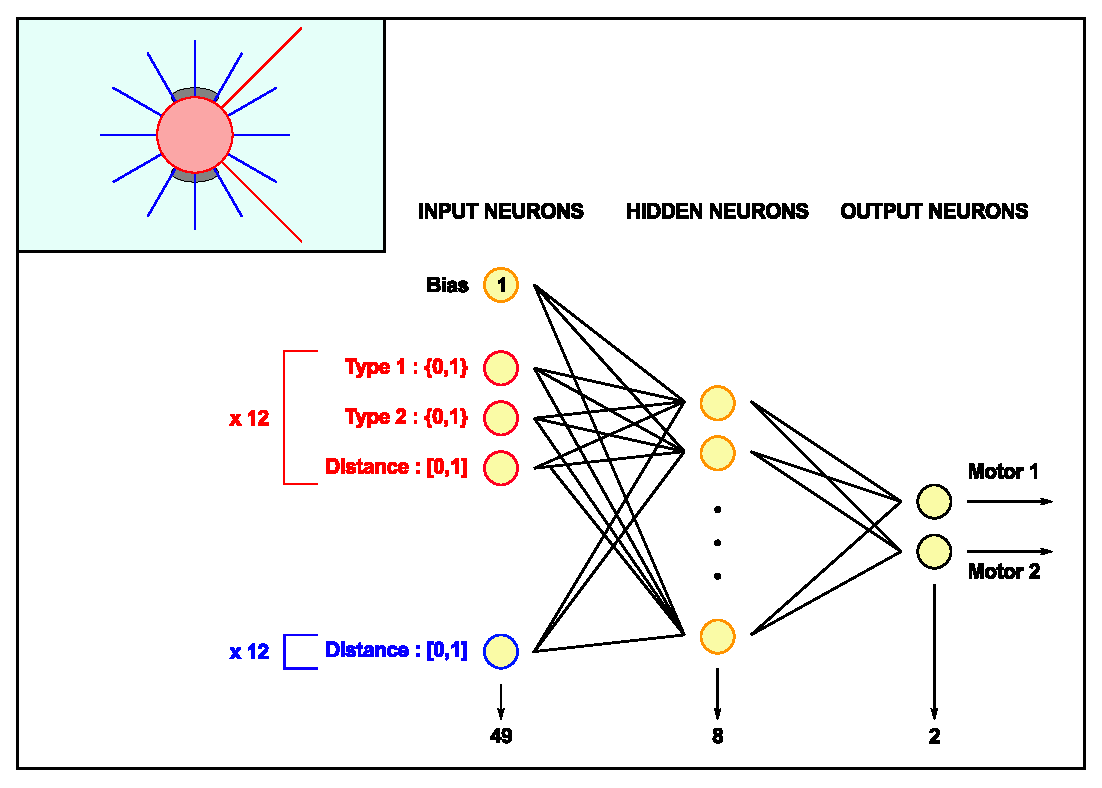
\includegraphics[scale = 0.5]{fig/ArticleBio1/Fig2.eps}
          \caption{\textbf{Diagram of the simulated robotic agent used in the simulation (inset) and its neural network controller.}
          The blue lines represent the 12 proximity sensors and the red lines represent the front camera. Inputs "Type 1" and "Type 2" are two boolean values used to represent the type of the agent (encoded with two bits) recognized by the camera ray.}
        \label{fig:robotDescription}
      \end{figure}


    \subsubsection{Simulating Artificial Evolution} 
    \label{artificialEvolution}
      To simulate evolution, we use an evolutionary algorithm to evolve the genome of the hunters. This genome is comprised of a collection of 410 real values in the range \([0,1]\), one for each of the neural network's weights, and is initially randomized for each individual in the population. In order to obtain its fitness, each individual is successively paired five times with a partner randomly chosen each time (except itself) in the arena presented in the Experimental Setup subsection, for an evaluation round of 20.000 time steps. The payoff of the evaluated individual at the end of a round is given by the total amount of food it has managed to obtain by killing prey in this round. As this quantity depends heavily on the initial conditions (random initial positions of the prey), five simulations are performed for each pair of individuals. The individual's fitness is then obtained by computing the sum of payoffs averaged over the total number of simulations for the individual. In this case the number of simulations is 25, with 5 partners and 5 simulations with each partner.

      Experiments were conducted using a Wright-Fisher model~\parencite{Wright1931} with constant population size (20 individuals), which is commonly known as a fitness-proportionate selection method in evolutionary robotics~\parencite{Eiben2003}. Using this model, the population of the next generation is formed by a random sampling of offspring from the previous generation, with the probability of sampling a particular parent proportional to the parent's fitness. Each offspring is simply a mutated clone of its parent; recombination is not included in our simulation. Consequently, new genotypes appear only through mutation. These mutations are performed using a Gaussian function, with a standard deviation of \(2 \times 10^{-1}\) and a mutation probability of \(5 \times 10^{-3}\). Each experiment lasted 3000 generations. All simulation parameters are summarised in Table~\ref{table:tableParameters}.

      \begin{table}[ht]
        \centering
          \caption{\textbf{Simulation parameters.}}
          \begin{tabular}{|l|l|c|}
            \hline
            \multicolumn{2}{|l|}{\textbf{Parameter}} & \textbf{Value} \\
            \hline
            \textbf{Evolutionary Algorithm} & & \\
            \hline
            & Selection method & Fitness-proportionate \\
            \hline
            & Population size & 20 \\
            \hline
            & Gene mutation probability & \(5 \times 10^{-3}\) \\
            \hline
            & Mutation operator & Gaussian \(\mathcal{N}(0, 0.01)\) \\
            \hline
            & Number of partners & 5 \\
            \hline
            & Number of simulations per pair & 5 \\
            \hline

            \textbf{Artificial Neural Network} & & \\
            \hline
            & Input neurons & 61 \\
            \hline
            & Hidden neurons & 8 \\
            \hline
            & Output neurons & 2 \\
            \hline
          \end{tabular}
        \label{table:tableParameters}
      \end{table}

  \subsection{Results}
  \label{sec:results}
    \subsubsection{Starting with a population of hare hunters}
      In order to explore the evolutionary transition between the risk-dominant equilibrium (hare hunting) and the payoff-dominant equilibrium (cooperative stag hunting), individuals first evolved in an environment composed solely of hares. This ensured that the populations initially reached the solitary equilibrium. Only then did we add stags and study the dynamics of evolution. Fig.~\ref{fig:hareHuntersRob}(a) shows the evolution of the mean percentage of stags hunted successfully (i.e., hunted cooperatively) out of the total number of prey hunted over time for 30 independent runs. Fig.~\ref{fig:hareHuntersRob}(b) shows the mean proportion of each type of prey hunted during the last generation of each run. Stag hunting evolved in only one run out of $30$ and even in that run accounted for less than 30\% of the total number of prey hunted. In the other $29$ runs, the individuals hunted only hares as they had previously evolved to do. These simulations demonstrate that the evolution of collective hunting is very unlikely when the population is composed of individuals who are already efficient solitary hunters.

      \begin{figure}[hbtp]
        \centering
          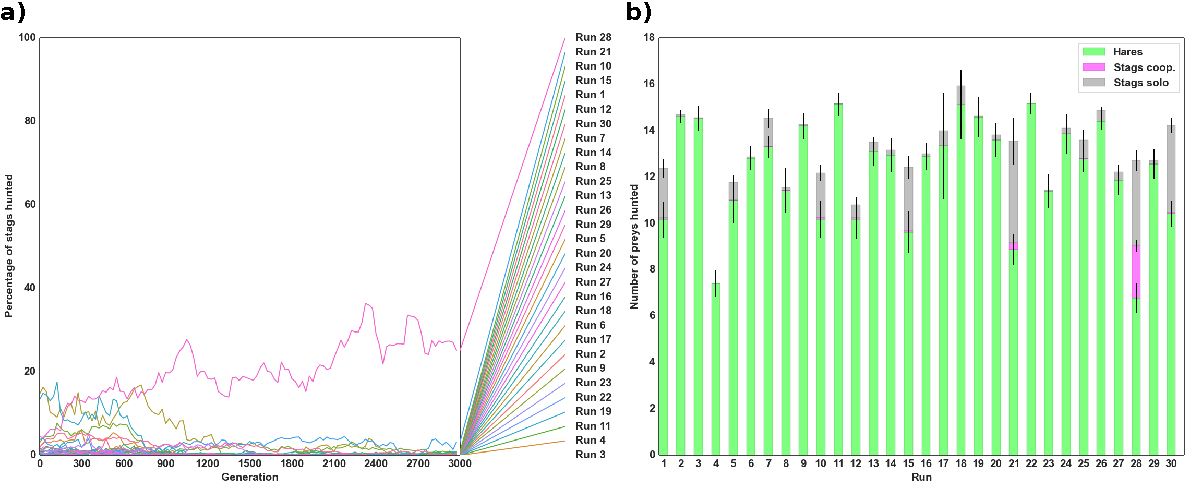
\includegraphics[scale = 1]{fig/ArticleBio1/Fig3.eps}
        \caption{\textbf{Evolution of cooperation in a robotic simulation with an initial hare-hunting strategy.} 
        {\em (a)}~Evolution of the mean percentage of stags hunted successfully (i.e. cooperatively) with respect to the total number of prey hunted. {\em (b)}~Mean number of prey hunted during the last generation of evolution for each independent run. The bottom green bar represents the number of hares hunted, the middle pink bar the number of stags hunted successfully (cooperatively), and the top grey bar the number of failed hunts (stags hunted alone). The standard deviation for each quantity is shown by black lines. The population for each of the 30 independent runs was previously evolved in an environment with only hares. Rewards were 50 for a hare, 0 for a stag hunted alone, and 500 for a stag hunted cooperatively as presented in Table~\ref{table:tableRewardsInitial}. The number of prey ($18$) was kept constant throughout the simulation by replacing killed prey by a prey of the same type.}
        \label{fig:hareHuntersRob}
      \end{figure}

      For comparison we simulated the same scenario using the standard game-theoretic version of the stag hunt, where the expression of the two types of behaviour was encoded by a single binary locus. Each individual in the population initially possessed the allele for hare hunting (Fig.~\ref{fig:hareHuntersTheo}).

      \begin{figure}[hbtp]
        \centering
            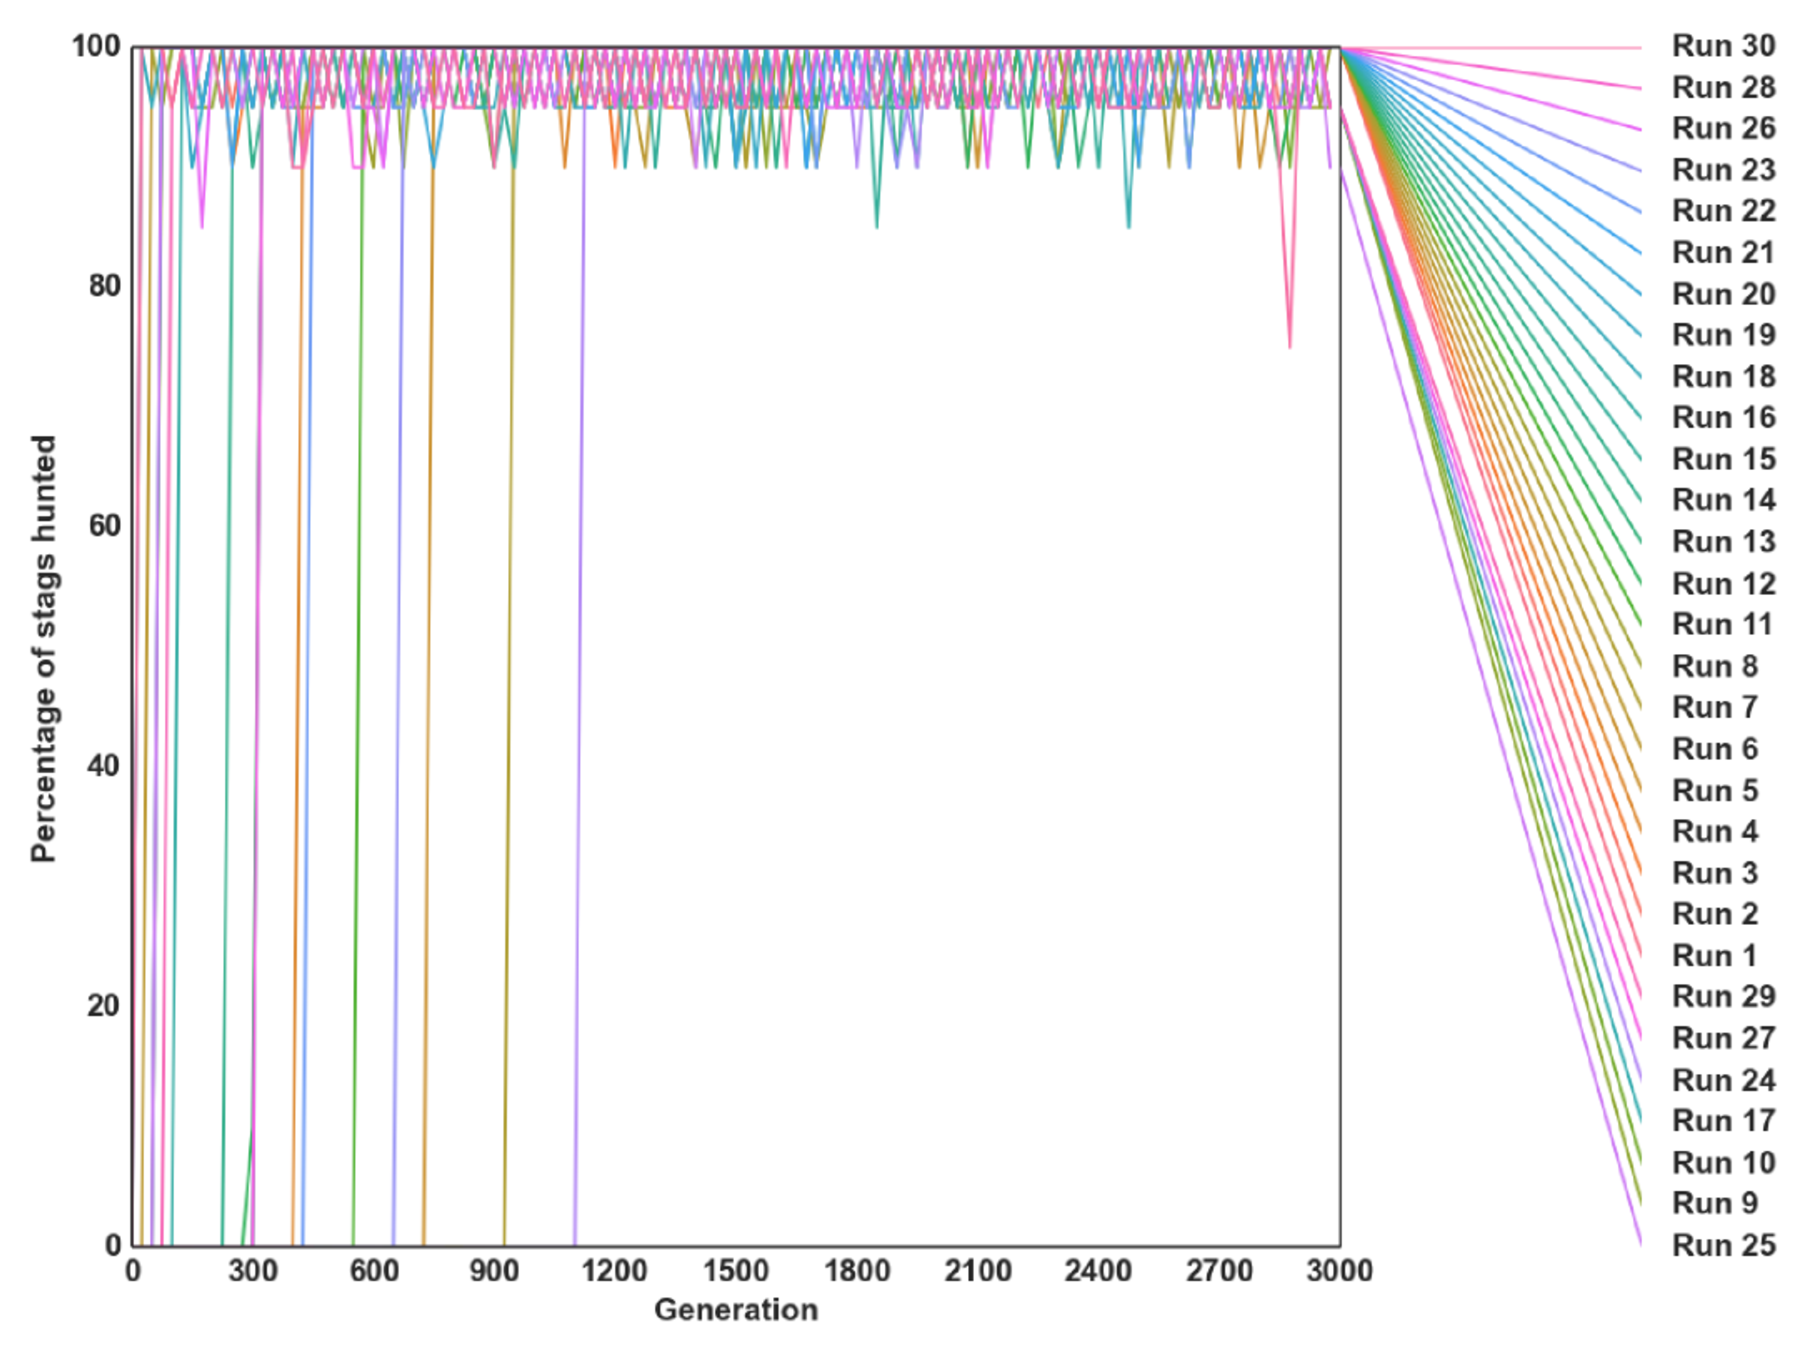
\includegraphics[scale = 0.35]{fig/ArticleBio1/Fig4.eps}
        \caption{\textbf{Evolution of cooperation in a game-theoretic simulation with an initial hare-hunting strategy.} 
        Evolution of the mean percentage of stags hunted successfully (i.e. cooperatively) with respect to the total number of prey hunted when starting with a population of hare hunters for 30 independent runs. Rewards were 50 for a hare, 0 for a stag hunted alone, and 500 for a stag hunted cooperatively as presented in Table~\ref{table:tableRewardsInitial}.}
        \label{fig:hareHuntersTheo}
      \end{figure}

      Here the transition to collective hunting occurred in each of the 30 independent runs and this strategy then remained stable. This result differs drastically from the results of our robotic simulations in which this transition never fully occurred (Mann-Whitney U test on the proportion of stags hunted successfully during the last generation, {\em p}-value \textless 0.001).


    \subsubsection{Starting with a random initial population}
      In a second experiment, we wanted to investigate the evolution of hunting strategies "from scratch", with the individuals' genotypes initialized with random values, rather than evolved with a specific hunting strategy. Fig.~\ref{fig:initialRandom} shows the mean percentage of stags hunted over time and the mean number of prey hunted during the last generation. We observed the transition to a clearly cooperative strategy in a single run, while in two other runs, 50\% of prey hunted were stags. In the $27$ remaining runs the proportion of stags hunted was less than 25\%. In comparison, in simulations using the standard game-theoretic version of the stag hunt where individuals are initially unable to hunt, stag hunting evolved and remained stable in every run (see supporting information, Fig.~\nameref{S1_Fig}).

      \begin{figure}[hbtp]
        \centering
          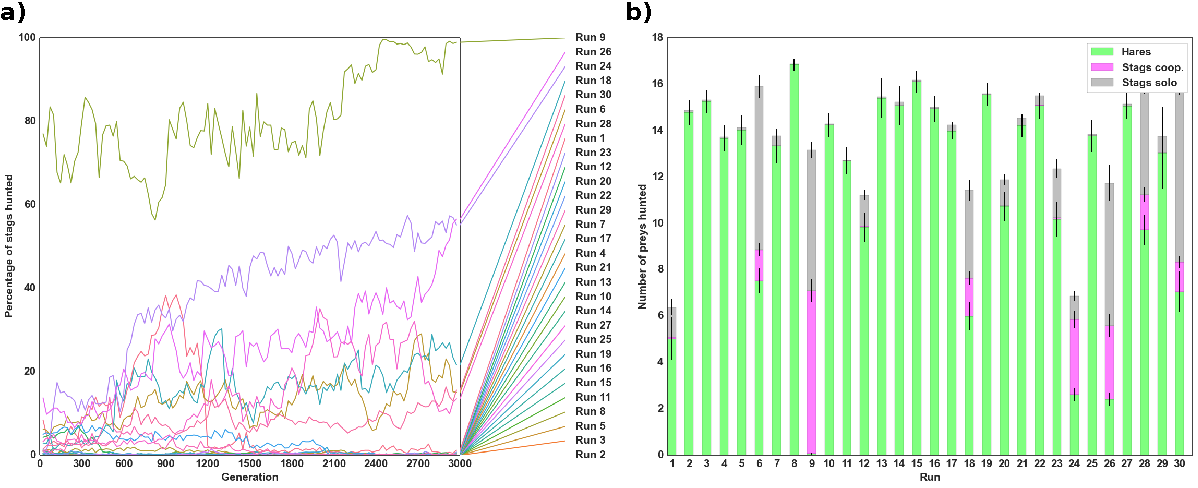
\includegraphics[scale = 1]{fig/ArticleBio1/Fig5.eps}
        \caption{\textbf{Evolution of cooperation with no initial hunting strategy.} 
        {\em (a)}~Evolution of the mean percentage of stags hunted successfully (i.e. cooperatively) with respect to the total number of prey hunted in a robotic simulation. {\em (b)}~ Mean number of prey hunted during the last generation of evolution for each independent run. The bottom green bar represents the number of hares hunted, the middle pink bar the number of stags hunted successfully (cooperatively) and the top grey bar the number of failed hunts (stags hunted alone). The standard deviation for each quantity is shown by black lines. Rewards were 50 for a hare, 0 for a stag hunted alone, and 500 for a stag hunted cooperatively, as presented in Table~\ref{table:tableRewardsInitial}. The number of prey ($18$) was kept constant throughout the simulation by replacing killed prey by a prey of the same type.}
        \label{fig:initialRandom}
      \end{figure}

      The above experiments show that mechanistic constraints have a critical effect on the evolution of coordinated collective actions. In a simple game-theoretic analysis in which the hunting strategy is encoded by a single binary gene, collective behaviour systematically evolved. However, in a setting where the hunting strategy was determined by a more complex artificial neural network, cooperative behaviour evolved in fewer than 10\% of cases. These results encourage further exploration into the evolutionary origin of coordinated collective actions and the mechanisms which may facilitate their evolution. In the following section, we explore two such mechanisms.


    \subsubsection{When stags can be hunted alone}
    \label{successfulCooperation}
      In the next experiment, food was also rewarded for hunting a stag in a solitary fashion so that cooperative behaviour did not entail a risk. We wanted to study whether hunting a stag alone could act as a transition towards the evolution of the collective strategy. Hunting a stag alone was given the same reward as hunting a hare (Table~\ref{table:tableRewardsStagAlone}), differing from classical models of the stag hunt.

      \begin{table}[ht]
        \centering
          \caption{\textbf{Food rewards for hunting different prey.}}
          \begin{tabular}{|l|r|c|}
            \hline
            \multicolumn{2}{|l|}{\textbf{Prey}} & \textbf{Food Reward} \\
            \hline
            Hare & \textit{alone} & 50 \\
            \hline
            & \textit{coop.} & 50 \\
            \hline
            Stag & \textit{alone} & 50 \\
            \hline
            & \textit{coop.} & 500 \\
            \hline
          \end{tabular}
          \begin{flushleft} The reward depends on whether these prey were hunted alone or cooperatively. There is a reward for stags hunted alone in this case.
          \end{flushleft}
        \label{table:tableRewardsStagAlone}
      \end{table}

      Fig.~\ref{fig:graphSolo} shows the results of robotic simulations where individuals initially evolved to hunt hares (as in Fig.~\ref{fig:hareHuntersRob}). As expected, the evolution of collective hunting was significantly facilitated when the risk of hunting stags alone was removed (Mann-Whitney, {\em p}-value \textless 0.001). The populations completely switched to hunting stags in two runs out of 30, and in three other runs, more than 50\% of the prey hunted were stags, with a large part of the prey hunted cooperatively in each of these runs. However, in most of the runs (25 out of 30), the evolved strategy was to hunt both types of prey in a solitary fashion. From these results, it entails that the individuals are still hindered by the evolution of a successful coordination strategy.
      
      \begin{figure}[hbtp]
        \centering
          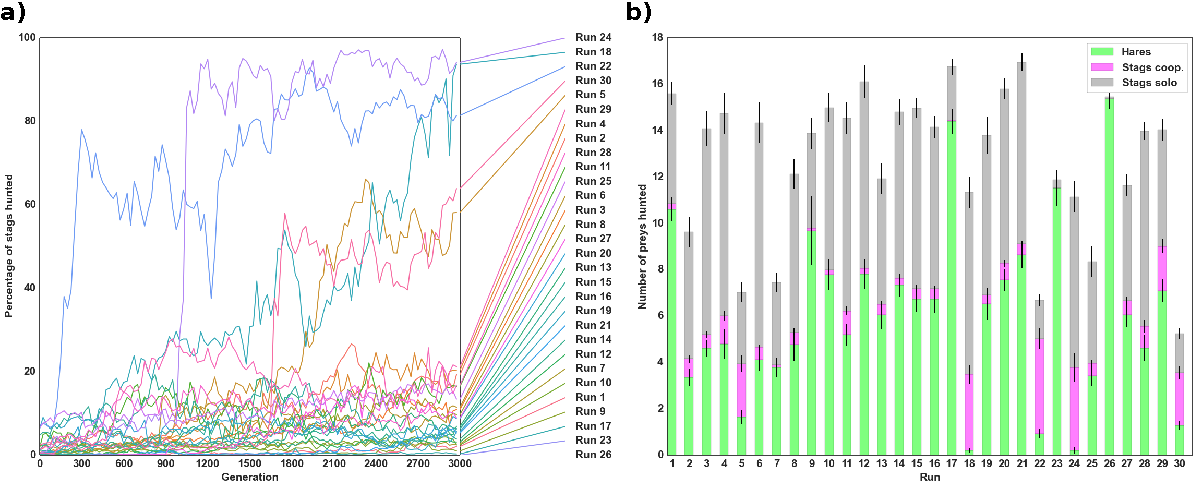
\includegraphics[scale = 1]{fig/ArticleBio1/Fig6.eps}
        \caption{\textbf{Evolution of cooperation with an initial hare-hunting strategy and a reward for solitary stag hunting.}
        {\em (a)}~ Evolution of the mean percentage of stags hunted successfully (i.e. cooperatively) with respect to the total number of prey hunted in a robotic simulation. {\em (b)}~ Mean number of prey hunted during the last generation of evolution for each independent run. The bottom green bar represents the number of hares hunted, the middle pink bar the number of stags hunted cooperatively and the top grey bar the number of stags hunted alone. The standard deviation for each quantity is shown by black lines. The population for each of the 30 independent runs was previously evolved in an environment with only hares. Rewards were 50 for a hare, 50 for a stag hunted alone, and 500 for a stag hunted cooperatively as presented in Table~\ref{table:tableRewardsStagAlone}. The number of prey ($18$) was kept constant throughout the simulation by replacing killed prey by a prey of the same type.}
        \label{fig:graphSolo}
      \end{figure}


    \subsubsection{The role of genetic relatedness}
      Genetic relatedness among social partners is known to influence the evolution of many types of social traits~\parencite{Hamilton1964}. In particular,~\parencite{Skyrms2004} showed how it can facilitate the evolution of cooperation in a stag hunt game~\cite[chapter 3]{Skyrms2004}. It can yield more frequent interaction between cooperators, which in turn increases their probability of benefiting from cooperative behaviour. In order to include this mechanism, we considered an extreme situation in which each individual is always paired with a clone of itself, known as "clonal selection" in robotics, ensuring a maximal genetic relatedness of 1.

      These results show that genetic relatedness has a positive effect on the evolution of cooperation (Fig.~\ref{fig:graphAltruism}). In four out of 30 runs the population evolved the cooperative strategy. Moreover, in two other runs, stags accounted for more than 75\% of prey hunted, as compared to less than 25\% without relatedness (Mann-Whitney, {\em p}-value \textless 0.005). When the initial population was random, rather than only hare hunters (see supporting information, Fig.~\nameref{S2_Fig}), the positive effect of genetic relatedness was also observed in 12 out of 30 runs, where more than 50\% of prey hunted were stags.

      \begin{figure}[hbtp]
        \centering
          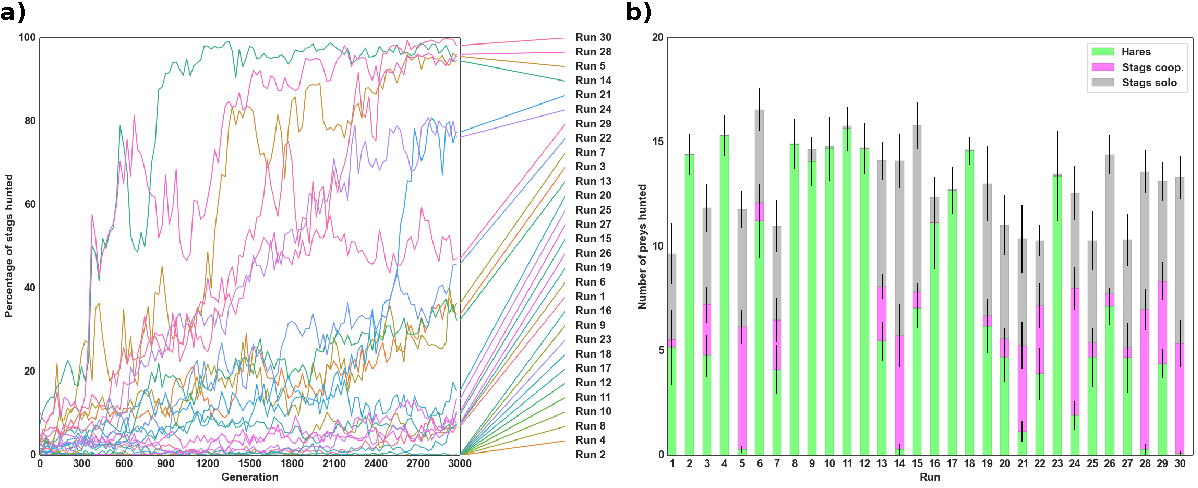
\includegraphics[scale = 1]{fig/ArticleBio1/Fig7.eps}
        \caption{\textbf{Evolution of cooperation under maximal genetic relatedness with an initial hare-hunting strategy.} 
        {\em (a)}~ Evolution of the mean percentage of stags hunted successfully (i.e. cooperatively) with respect to the total number of prey hunted in a robotic simulation. {\em (b)}~ Mean number of prey hunted during the last generation of evolution for each independent run. The bottom green bar represents the number of hares hunted, the middle pink bar the number of stags hunted successfully (cooperatively) and the top grey bar the number of failed hunts (stags hunted alone). The standard deviation for each quantity is shown by black lines. The population for each of the 30 independent runs was previously evolved in an environment with only hares. The genetic relatedness between paired individuals was 1. Rewards were 50 for a hare, 0 for a stag hunted alone, and 500 for a stag hunted cooperatively as presented in Table~\ref{table:tableRewardsInitial}. The number of prey ($18$) was kept constant throughout the simulation by replacing killed prey by a prey of the same type.}
        \label{fig:graphAltruism}
      \end{figure}

  \subsection{Discussion}
  \label{discussion}
    There is a profound difference between evolutionary game-theoretic and robotic simulations of the stag hunt. Using identical model parameters, the transition from the solitary equilibrium to the social equilibrium always occurred in game-theoretic simulations, but was extremely unlikely in robotic simulations, occurring in $1$ run out of $30$. The complexity of the mapping between genotype and phenotype is responsible for much of this contrast. Individuals involved in a coordination game such as the stag hunt face a chicken \& egg problem: the cooperative behaviour must be beneficial in order to evolve, but no individual can benefit from this behaviour unless the behaviour is already expressed by other individuals. When binary variation at a single genetic locus encodes the expression of the solitary or cooperative strategy, a single mutation is sufficient for a cooperative mutant to appear in a resident population of solitary individuals. In a finite population, demographic stochasticity can then lead to the rise of cooperators above the invasion threshold, at which point natural selection leads to their fixation, switching from a solitary equilibrium to a social one. In contrast, in our robotic simulations, the mapping between genotype and phenotype is more complex. Adopting the social strategy entails both a modification of the preferred hunting target and the ability to coordinate with others. Thus, several mutations are necessary for the appearance of full-fledged cooperative behaviour. As several individuals must carry these multiple mutations for the behaviour to become beneficial, the transition to the cooperative equilibrium is nearly impossible.

    In particular, in our robotic simulations we were able to observe that coordination entails a specific and rather complex behaviour. Fig.~\ref{fig:behaviourTraces} (see also supporting information, Movie S1\_Movie) shows the behaviours evolved by the best individuals in the cooperative run shown in Fig.~\ref{fig:initialRandom} (Run $9$). The solution they evolved for coordination was to circle around one another, allowing each of them to constantly see their partner while both moving closer to a stag. This behaviour was replicated in every cooperative run. We thus observed the evolution of an ingenious (given the agents' limited capabilities) and complex hunting strategy. These findings demonstrate that the practical mechanics of behaviour can have important evolutionary consequences, and that models which ignore these properties may lead to misleading predictions.

    Moreover, the evolution of cooperation is also strongly impacted by ecological features. Social hunting poses a bootstrapping problem because it entails both a modification of the preferred hunting target and an ability to coordinate with others. Its evolution can be facilitated, therefore, if hunters have a reasonable probability of hunting the same prey as their partner, just by chance, with no need of active coordination. Biologically, this could occur if hunters live in a dense social environment (with many other hunters in the vicinity), and/or if the density of prey is low, such that the likelihood of ending up on the same prey is large. To test this possibility, we conducted additional experiments where the density of prey was varied. The number of prey was whether (1) decreased from $18$ to $6$ or (2) increased from $18$ to $30$. The population was initially constituted of hare hunters and we kept the same ratio of prey as in previous experiments (i.e. 50\% of hares and 50\% of stags). We show (see supporting information, Fig.~\nameref{S3_Fig}(a)) that when the number of prey is decreased ($6$) the transition to a cooperative strategy is facilitated (Mann-Whitney, {\em p}-value \textless 0.05) as in $9$ runs out of $30$, more than $30$\% of the prey hunted are stags. In comparison, a higher density of prey ($30$) entails that it is impossible to evolve cooperation (see supporting information, Fig.~\nameref{S3_Fig}(b)). These results reinforce our claim that the practical mechanics of coordination are crucial in understanding the evolution of cooperation. In particular, here, the precise ecological situation faced by individuals plays a key role in the transition to the collective equilibrium.

    Finally, the complexity of coordination suggests that the recycling of a previously evolved trait could be necessary for the transition to cooperation, i.e. individuals could coordinate thanks to behavioural features that may not have been selected for cooperation at first. Such features could include the evolution of communication, or a leader-follower strategy. The role of both of these behaviours has already been studied in real-life stag hunt type interactions in chimpanzees and human children~\parencite{Bullinger2011, Duguid2014}, and there is an already extensive literature in evolutionary robotics on their role in the evolution of collective actions~\parencite{Trianni2007, Mitri2009, Solomon2012, Ferrante2015}. This offers some directions for future works on this problem.


    \begin{figure}[hbtp]
      \centering
        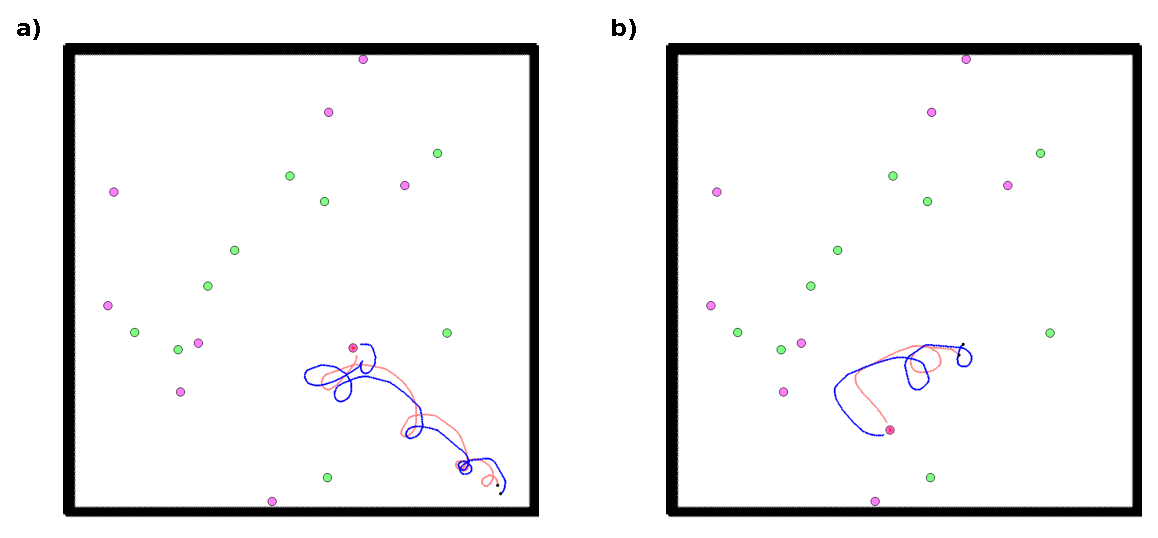
\includegraphics[scale = 1]{fig/ArticleBio1/Fig8.eps}
      \caption{\textbf{Snapshots of a simulation after two hunts.}
      In each of these snapshots, we show the path travelled by each hunter (in different colours) since their last prey was hunted. The black dots represent the positions of the hunters at their last kill. The red star on the stag (pink circle) converged on by the hunters indicates not only that the prey was killed but, more importantly, that it was killed cooperatively by the two hunters.}
      \label{fig:behaviourTraces}
    \end{figure}


  \subsection{Supporting Information}
    \begin{figure}[hbtp]
      \centering
        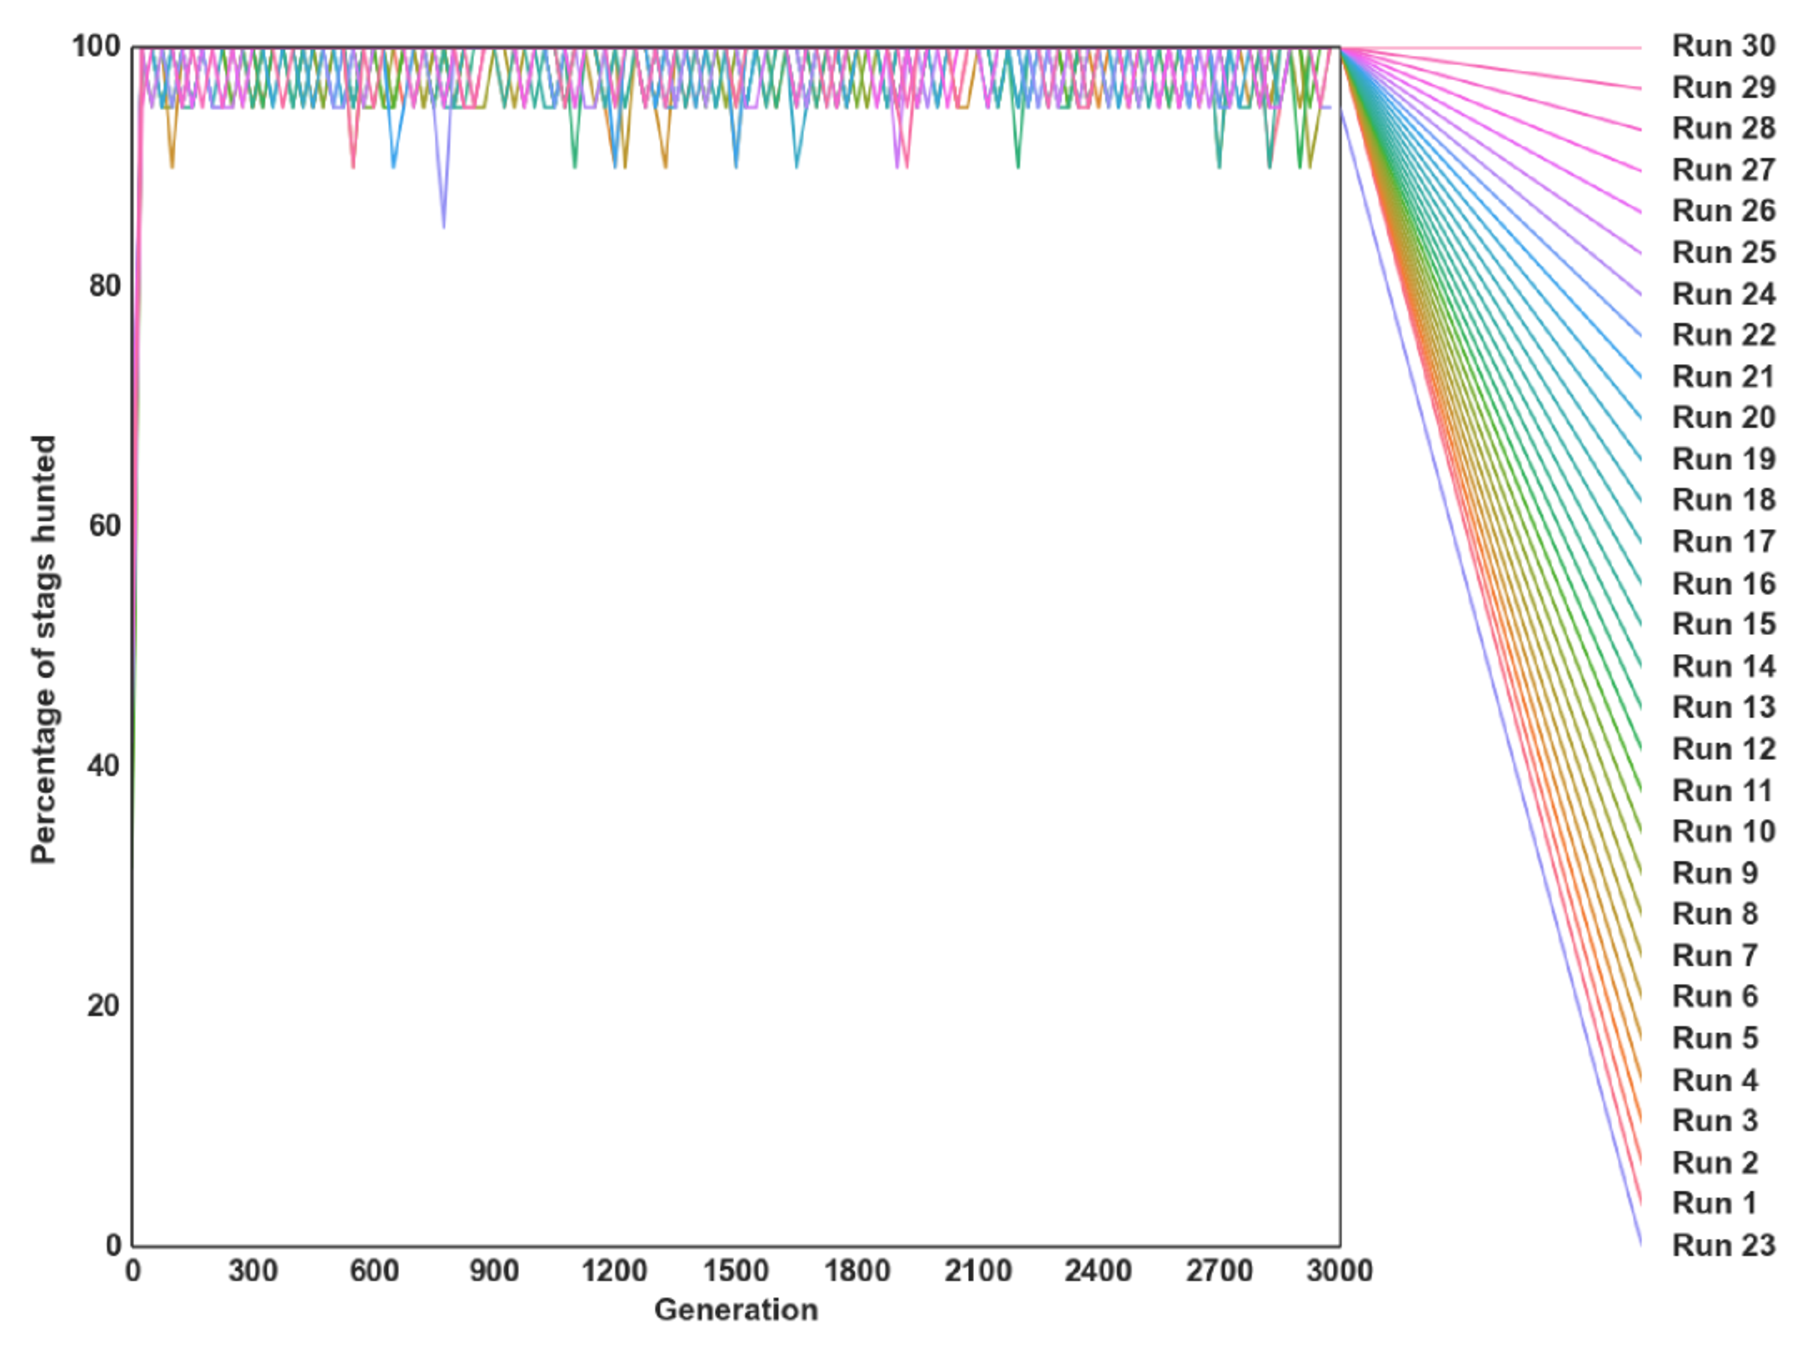
\includegraphics[scale = 1]{fig/ArticleBio1/S1_Fig.eps}
      \caption{\textbf{Evolution of cooperation in a game-theoretic simulation with an initial hare-hunting strategy.} 
      Evolution of the mean percentage of stags hunted with respect to the total number of prey hunted where individuals are initially unable to hunt for 30 independent runs. Rewards were 50 for a hare, 0 for a stag hunted alone, and 500 for a stag hunted cooperatively.}
      \label{S1_Fig}
    \end{figure}

    \begin{figure}[hbtp]
      \centering
        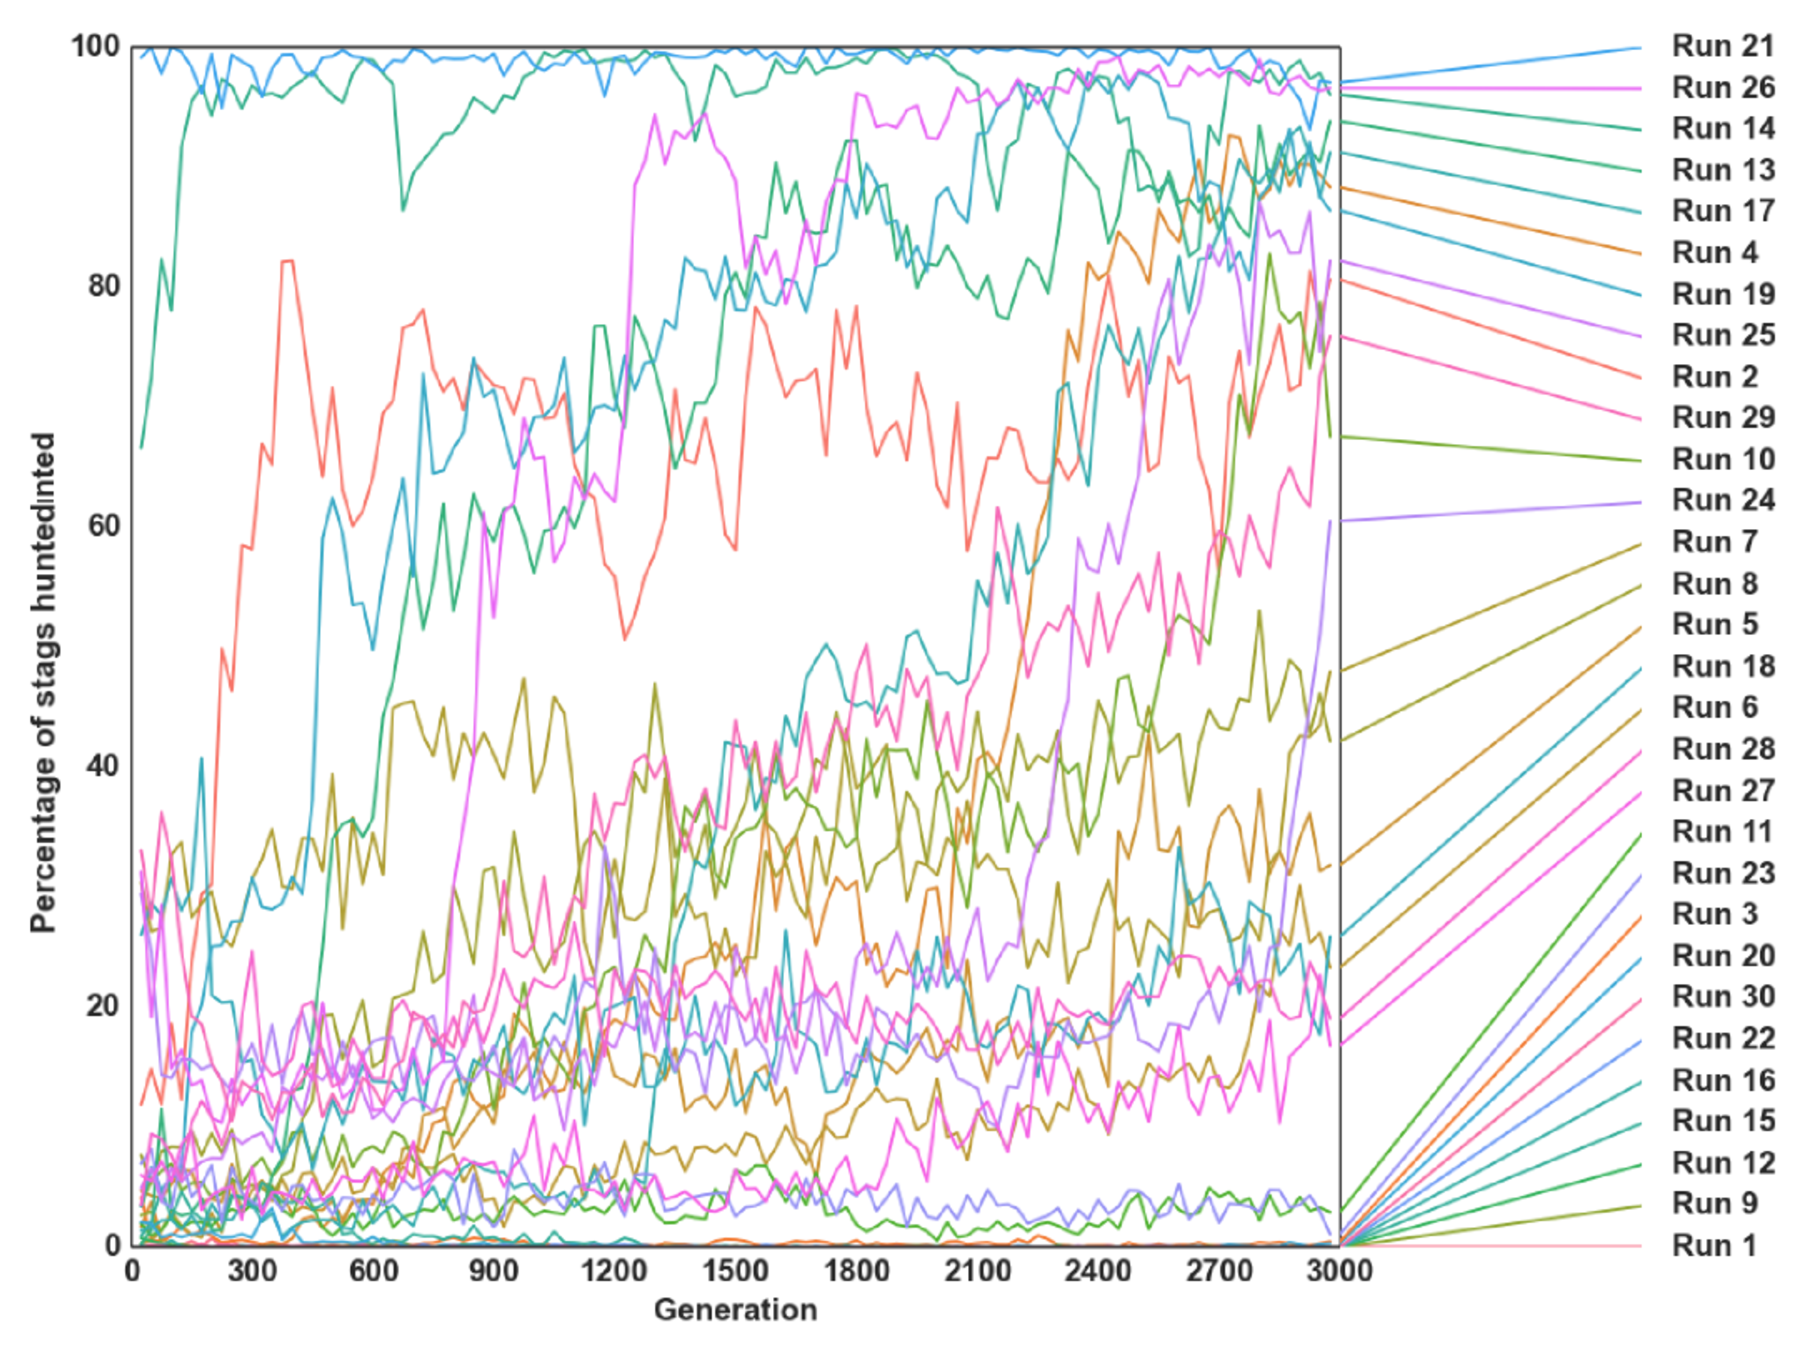
\includegraphics[scale = 1]{fig/ArticleBio1/S2_Fig.eps}
      \caption{\textbf{Evolution of cooperation under maximal genetic relatedness with no initial hunting strategy.}
      Evolution of the mean percentage of stags hunted with respect to the total number of prey hunted in a robotic simulation. The genetic relatedness between paired individuals was 1. Rewards were 50 for a hare, 0 for a stag hunted alone, and 500 for a stag hunted cooperatively as presented.}
      \label{S2_Fig}
    \end{figure}

    \begin{figure}[hbtp]
      \centering
        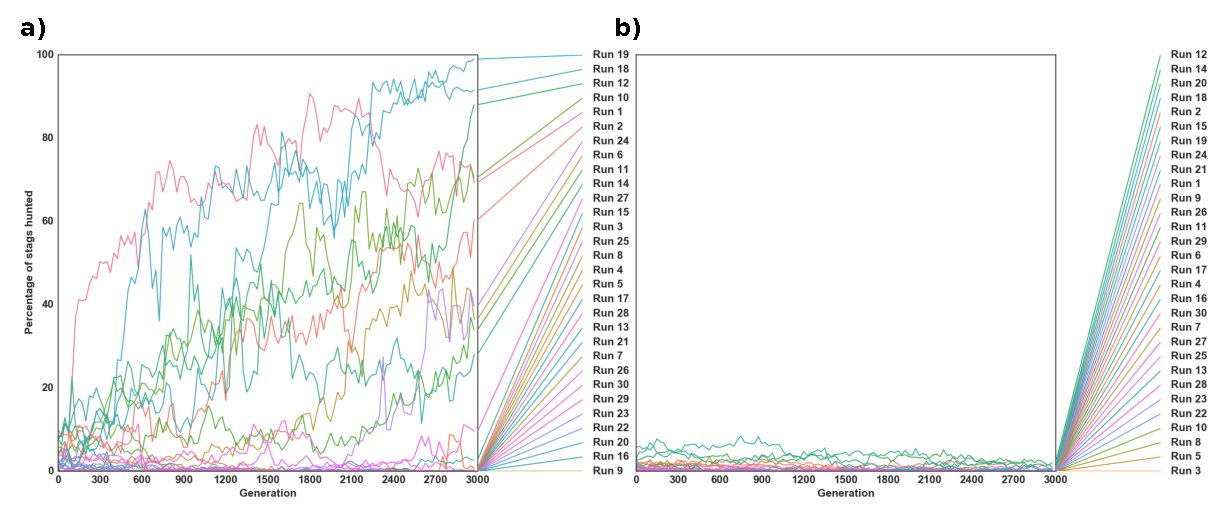
\includegraphics[scale = 1]{fig/ArticleBio1/S3_Fig.eps}
      \caption{\textbf{Evolution of cooperation with an initial hare-hunting strategy and a varied density of prey.} 
      Evolution of the mean percentage of stags hunted successfully (i.e. cooperatively) with respect to the total number of prey hunted in a robotic simulation when the number of prey was {\em (a)} $6$ and {\em (b)} $30$. The population for each of the 30 independent runs was previously evolved in an environment with only hares. Rewards were 50 for a hare, 0 for a stag hunted alone, and 500 for a stag hunted cooperatively as presented in Table~\ref{table:tableRewardsInitial}. The number of prey was kept constant throughout the simulation by replacing killed prey by a prey of the same type.}
      \label{S3_Fig}
    \end{figure}

% \chapter{The optimization of collective actions by individual selection}
\label{chapter:C1_article2}

\minitoc[n] % minitoc without title

In this Chapter, we investigate the influence of the nature of coordination behaviours on the optimization of collective behaviours. This Chapter is presented as a draft for a journal article which will be submitted before the end of the year.

% \begin{quote}
%   \fullquote{Bernard2016a}
% \end{quote}

% TODO: peut-être un peu mieux gérer la transition entre les chapitres ?

In the previous Chapter we showed that the evolution of collective actions was hindered by the evolution of coordination. Here we are more interested on the impact of coordination on the transition from different collective equilibria. More precisely, these behaviours allow to reap benefits that would not be obtained in a solitary manner (e.g. collective hunting). However, because they require coordination, it is not clear how these collective behaviours are reached. In particular, the need for multiple individuas to coordinate implies that several equilibria evolve may evolve. Because benefits are reaped through collective action, a single individual would not benefit by deviating from the evolved equilibrium. This means that mutant acting toward a different equilibrium could not be selected. This would be the case even if the equilibrium would be more advantageous for the group. In consequence, these collective equilibria are stable when evolved but the evolution a particular equilibrium is not straight foward. This raises the issue of the optimization of collective actions, i.e. the transition toward an optimal equilibrium when another collective equilibrium has already been evolved.

One classical mechanism to solve this issue is that group selection. Because those behaviours are beneficial at the level of the group, then this should mean that they are selected at the same level. However, we want to study if collective behaviours could be optimized by individual selection only. To that end, we choose to model the example of collective hunting. In particular, we use a similar model as the one in Chapter~\ref{chapter:C1_article1}. Namely, individuals are evolved in an environment where they can hunt two differently rewarding types of prey: \emph{boar} and \emph{stag}. Each type of prey corresponds to a different collective equilibrium: suboptimal for the boar and optimal for the stag. Our goal is thus to study the transition from the suboptimal equilibrium (i.e. boar hunting) to the optimal equilibrium (i.e. stag hunting).

We reveal that under simple ecological features (only two prey in the environment), the transition to the optimum is impossible. However, under more realistic assumptions where the individuals have to choose between multiple prey, then the optimal equilibrium is evolved in $8$ replications out of $30$. In particular, the individuals now have to coordinate in order to achieve cooperation. This means that they need to react to each other behaviour. In consequence, they react to a mutant's behaviour which may allow to reap the benefits of stag hunting. However, the coordination strategy observed in one where both individuals try to simultaneously choose the prey on which to hunt. They thus adopt very symmetrical behaviours.

We then increase the complexity of the neural networks to study the impact of the evolution of a more complex coordination strategy. We observe the evolution of a more efficient asymmetrical strategy where the individuals adopt two different roles: the \emph{leader/follower} strategy. In this case, we reveal that the transition to the optimum is facilitated as stag hunting evolves in $24$ replications out of $30$. In this strategy, only the leader chooses the prey and the follower goes on the same prey. In consequence, while previously choosing to hunt a stag was a collective decision making problem, it is now an individual problem. This means that a mutant leader going on a stag is now sufficient for both individuals to reap the benefits of stag hunting. Furthermore, the leader/follower strategy evolved because it was more efficient. Thus we showed that the evolution of an individually adaptive coordination strategy could lead to the optimization of a collective behaviour.

\part{Designing Cooperative Robots in Evolutionary Robotics}


\chapter{Design}
\label{chapter:design}

\epigraph{I need to find a clever epigraph.}{--- \textup{Arthur Bernard}}

\minitoc[n] % minitoc without title

In this part of the manuscript, we aim at designing cooperative heterogeneous robots in a multirobots system by using evolutionary robotics. In particular, we are interested in the evolution of coordination behaviours and the influence of teams' genetic composition in the emergence of more efficient collective behaviours~\parencite{Waibel2009}. Namely, we want to study the impact of aclonal approaches~\parencite{Quinn2001} on (1) the capacity to evolve cooperation and (2) the efficiency of the cooperative solutions.

% as well as the evolution of specialization by way of genotypic polymorphism.

In the context of designing multirobots systems, our approach is to use evolutionary robotics. While using evolutionary processes for engineering is not new, this approach is still recent when it comes to designing robotic systems. As any given method, evolutionary robotics comes with assumptions and constraints. In this Chapter, we thus want to review the features (both negative and positive) of evolutionary robotics with regards to multirobots systems and motivate the choice of using this design method. First we give a quick overview of multirobots systems as well as their main advantages when compared to single robots. In particular, we emphasize on the design choices that come with creating those systems and what they imply. Additionally, we present a few applications of multirobots systems that are either seminal and/or noteworthy. Then we focus on the control of collective robotics systems. In particular, we briefly mention how the issue of control is addressed in single robots. We can thus compare with the way this matter is tackled in multiple robots. There has indeed been a strong interest in taking inspiration from single robots to apply the same solutions to multirobots. This is obviously not so simple. In this way, we also reveal the particular challanges brought up by the control of multiple robots. Next we talk about the use of machine learning, and in particular reinforcement learning, to the automatic design of multirobots systems. We briefly mention the main reinforcement learning techniques used in the context of single robots before discussing how these techniques have been transferred to multirobots engineering. Our goal is thus to shed some light on the advantages and limits of such approaches. We then move to evolutionary techniques and how they have been applied to the design of multirobots systems. We thus expose the main differences with traditionnl learning in this context and quickly review the main results obtained in the design of collective behaviours. Finally, we conclude by motivating the choice of studying evolutionary robotics for the design of cooperative robots.


\section{Cooperative Robots for Collective Tasks}

  \subsection{Multirobots Systems} 

    Multirobots systems (MRS), or sometimes multi-agent robotics~\parencite{Dudek1996}, essentially gained fame during the 1980s. The main motivation was to use cooperation between robots in order to cope with tasks that classical single robots may not achieve. CEBOT and ACTRESS are often cited among the earliest successful MRS. CEBOT~\parencite{Fukuda1988} (for CELlular roBOTic system) is a decentralized architecture inspired by cellular organization. The organization of the system is dynamic and robots, which are coupled to one another, can reconfigure their structure under environmental changes. This system is based on a hierarchical organization where "master cells" (which are also robots) can communicate with other master cells and allocate subtasks to all of the agents in the system. In comparison, in ACTRESS~\parencite{Asama1989} (ACtor-based Robot and Equipments Synthetic System) the system is composed of three robots and three workstations. One of these workstations is operated by an human, another is used as image processing and the last one manages the environment. Given this heterogeneous group of six agents, the goal is for the robots to perform a purely collective task (i.e. that could not be achieved by a single robot) like pushing an object. This system raises the issue of achieving efficient communication between multiple levels of organization.

    MRS can be constitued of between two to a thousand of autonomous robots~\parencite{Rubenstein2014} depending on the task at hand. While it may seem counter-productive to develop and control several robots where a single robot could very well be sufficient, using a team of robots has several advantages among which~\parencite{Cao1997, Arkin1998}:

    \begin{itemize}
      \item{The parallel execution of multiple robots allows the task to be achieved faster.}
      \item{Using multiple robots can ensure robustness and reliability through \emph{redundancy}.}
      \item{It can be both cheaper and simpler to produce several simple robots compared to a single complex one (especially if the robot may suffer damages).}
      \item{It may be necessary to distribute several robots at the same time to complexte the task, in which case a single robot would simply not be sufficient.}
    \end{itemize}

    This implies that there are several crucial features that are often expected of MRS~\parencite{Parker1994}. However it is important to note that because applications vary greatly, MRS are very different in design. First, MRS are supposed to be \emph{adaptable} and \emph{flexible}. Most often, this adaptability is found at the agent level. Robots are indeed expected to react to environmental changes and, most importantly, to a change in others or induced by them. This also means that, in the lesser decentralized systems, the control system should adapt the global organization accordingly. Then, a MRS should be \emph{robust}. This implies that the system should not be too impacted by failure (and in particular individual failures). This is easier said than done but, as we previously said, this is also one of the main advantages of such an approach. Because robots are expected to be autonomous, it is possible to design the system so that a fault on one or several robots does not critically impact the whole system. This also means that in systems such as CEBOT, where some agents (in this case the "master cells") have a particular role, achieving full robustness is harder: the fault must be anticipated during design. And because MRS may handle several tasks as the same time, there must be a way to dynamically allocate the tasks according to the actual functionning robots. Finally, it is often expected of MRS to be fully \emph{autonomous}. This means that the system as well as all the agents that compose it should be able to act without human intervention. In particular, the system should be able to face the unexpected without human control for some time. All these features mean that MRS are most adequate for several classical robotics tasks, the most famous of which being: foraging, object transportation, localization and mapping or path planning~\parencite{Farinelli2004}.

    Because applications vary greatly, there is no canonical architecture for MRS~\parencite{Cao1997, Parker2008}. First, the control of a MRS can be \emph{centralized} or \emph{decentralized}. In a centralized architecture, a single agent is responsible for controlling the system. Thus while this agent has full knowledge other the whole system, it represents a critical point for failures. Therefore, this type of organization is rare in MRS~\parencite{Parker2008} and most use a decentralized approach. Decentralized architectures can be of two types: \emph{hierarchical} or \emph{distributed}~\parencite{Cao1997}. In a hierarchical architecture, the system is locally centralized and some agents are in charge of a group of other agents to organize the task at hand (e.g. CEBOT). In comparison, in a distributed system, all agents are equal w.r.t. control which, while robust, implies that it is harder to achieve coherence between every agents.

    One critical design choice we need to address given this thesis is team composition, which may be \emph{homogeneous} or \emph{heterogeneous}. In an homogeneous team, individuals are all identical in terms of both software (control) and hardware (morphology and sensors). In comparison, heterogeneous robots vary grealt between one another. Most works in MRS have often focused on homogeneous teams as it is more practical in terms of task allocation: because every agent is the same, they all can achieve the same tasks. In consequence it is also more resilient to failures. In comparison, it is more difficult for heterogeneous teams to achieve coordination~\parencite{Parker1994}. However, they can benefit from the differences between individuals to display more diverse coordination strategies. Designing heterogeneous systems gives rise to critical issues in the field of MRS~\parencite{Parker2008}:

    \begin{itemize}
      \item{How to achieve efficient communications between several different robots ?~\parencite{Jung2000}}
      \item{How to efficiently allocate tasks between agents with differing capabilities ?~\parencite{Parker2003}}
    \end{itemize}

    % À réfléchir: un bla bla sur les différentes façons de faire du task allocation et les différentes formes de communication ? Je pense pas que ça soit nécessaire mais si on a de la place... pourquoi pas ?

  \subsection{The Origin of Cooperation} 

    One of the main problems at the heart of designing a MRS is: how to achieve cooperation ? In their popular (though now ancient) review of the field, Cao and colleagues~\parencite{Cao1997} deemed this as one of the prime research axis in MRS. McFarland~\parencite{McFarland1996} argued that the design of cooperative robots could fall into two broad categories that he considered to be the same for group behaviours in nature: \emph{cooperative behaviour} and \emph{eusocial behaviour}. While this classification is more than doubtful for natural cooperative behaviours, its biological validity is not of real importance here. The more important point here is that since nearly the beginning of MRS, there has been an interest in taking inspiration from natural social behaviours for achieving coopration. Although without direct biological analogy, Parker~\parencite{Parker2008} classified the design of multirobots cooperation in two similar categories: \emph{intentionally cooperative} systems and \emph{collective swarm} systems. This categorization entails different manners in which to ensure cooperation.

    % but [McFarland] was mainly basing his argument on the work of Tinbergen~\parencite{Tinbergen1953} -> Really ?

    The intentionally cooperative MRS mostly comprised systems where agents have high knowledge about the other individuals' presence. They are capable of acting in accordance to others' actions and capabilities and may use communication to coordinate. In these MRS that McFarland simply classified as "cooperative behaviours", he defined an agent to be selfish. This means that cooperation comes from the maximization of the agent own utility. This paradigm is often caracterized by a more direct approach to cooperation. In particular, there is careful design on the manner with which robots can coordinate. Moreover, this approach is often well suited for MRS dealing with groups of heterogeneous robots, where the origin of cooperation represents a challenge by itself. From this it stems that this type of MRS sometimes takes inspiration from \emph{distributed artificial intelligence} (DAI). This field is mainly concerned with the design of distributed systems of intelligent agents~\parencite{Cao1997, Panait2005} and is generally considered to be divided in two major areas of studies: distributed problem solving (DPS) and multiagent systems (MAS). To summarize quickly, DPS is mostly concerned with solving problems with several agents. As such, some of its problematics are common to MRS (e.g. task allocation). However, because in DPS agents are considered to always be cooperative and are usually disembodied, few works can really contribute to MRS. In comparison, in MAS agents are often rational and as such are not de facto cooperators. Thus there is a strong emphasis on the collective interactions between agents. This is a reason why there has been consistent interest in game-theoretic approaches with MAS~\parencite{Rosenschein1985}. Therefore, MAS carry some theoretical ground for achieving cooperation in MRS. However, some have argued that MAS are not rooted enough in the physical world for them to make a powerful contribution to MRS~\parencite{Cao1997, Farinelli2004}. In particular, perfect sensory information is often assumed in MAS which may hinder direct transfer to robotics. For this reason, research in DAI tend to consider the mechanisms of coordination behaviours as a black box~\parencite{Parker1994}.

    % We believe selfishness is not necessarily associated with intionnally cooperation ?


    On the other end of the spectrum lies collective swarm~\parencite{Beni2005}, also called collective robotics~\parencite{Kube1993, Parker2008}. Although it could be argued that any MRS is a particular instance of collective robotics, we will make here the distinction as to not generate confusion w.r.t. the litterature. In this approach, the MRS is often constituted of a high number of robots (at least several dozens) which are all homogeneous and distributed agents. Also called "reactive collective robotics", collective swarm takes inspiration from the behaviours and organization of eusocial insects~\parencite{Wilson1998, Werfel2014}~\footnote{A more thorough presentation of eusociality and the altruistic behaviours of eusocial animals is given in Chapter~\ref{chapter:model}. Consequently, there will not be an extensive discussion on this subject here.}. More precisely, the study of eusocial insects led to the creation of the field of Swarm Intelligence~\parencite{Bonabeau1999, Zoghby2013}. This field consists of heuristics designed to solve algorithmic problems by taking inspiration from the natural collective behaviours. Some of the most famous algorithms that stemed from Swarm Intelligence are ant colony optimization (ACO)~\parencite{Dorigo2004a}, for which the most classical problem is to find the best travel route in a traveling salesman problem, and particle swarm optimization (PSO)~\parencite{Kennedy1995}, where candidate solutions to an optimization problem are modeled as particles moving through the search space. The main goal of swarm robotics is to design a large colony of decentralized and self-organized robots capable of high flexibility and robustness.

    Agents in a swarm are as simple as possible and constituted of very basic sensory capabilities. In particular, direct communication between robots is often inexistent. Instead, they rely on \emph{stigmergy}, where indirect communication is achieved by looking at other individuals' modification of the environment (e.g. the use of pheromones by ants in the natural world). Additionally, robots in a swarm are often largely unaware of the actions and internal states of others, basing their knowledge on proximity information. This implies that robots are not capable of achieving much on their own. Their role is really to be a part of the collective. In particular, the main concept of swarm robotics is that of \emph{emergence}\footnote{It is interesting to note that swarm robotics and individual-based modeling, which we presented in Chapter~\ref{chapter:model}, share a lot of similar key concepts. In particular, the concept of emergent collective behaviours between agents is one that is central to IBM.}. This means that we expect to see the appearance of global collective complexity from the local interactions between agents of the swarm, something which is also known as \emph{self-organization}. More precisely, swarm robotics are based on the principle of superadditivity~\parencite{Parker2008}, where the whole result (collective behaviour) is better than a simple sum of all its parts (the agents' behaviours). In consequence, the design of a swarm is focused on creating simple local behavioural rules that should allow the whole system to act in a collective way. It is as if cooperation is a side effect resulting from individual behaviours. This is obviously complex to design and time must not be critical. However, it also means that agents are cheaper to produce, deploy and control. Also, thanks to self-organization, the tasks covered by swarm robotics often require little to no \emph{a priori} assumptions. At the inception of collective robotics, this conception was really different from the "classical" design paradigm in robotics and especially in AI which emphasized on high reasoning and higher-levels of cognition~\parencite{Bonabeau1999}. While examples of swarm robotics systems are numerous we can quickly name a couple. One of the first examples of successful swarm robotics on real robots was the \emph{Nerd Herd} by Matarić~\parencite{Mataric1995}. With a group of $20$ identical robots with very simple individual capabitilies (mainly detection of obstacles and other robots) and a set of pre-programmed behaviours, she created a system capable of collective behaviours of flocking, surrounding, herding and foraging. Another interesting example is that of Swarm-bot~\parencite{Mondada2004, Dorigo2004, Mondada2005}. The goal was to engineer a swarm of simple identical robots capable of using self-assembly to navigate accross rough terrain and achieve different collective tasks.

    % -> This is not always that simple. Genre en swarm on peut faire plein de trucs globallement et des fois ya du knowledge (je crois). Et le swarm peut être classé en MAS (voir Panait2005)
    % -> Globalement frontière blurry encore une fois. On va assez vite parler de swarms pour des trucs qui répondent pas aux principes de base des swarms


\section{The Control of Collective Robots}

  Because robots are expected to cooperate and in some cases coordinate, there is a strong need for reactivity and adaptability in MRS~\parencite{Iocchi2001, Farinelli2004}. The fact that multiple individuals engage in a collective behaviour implies that the individuals act in a dynamic environment. To that end, the concept of \emph{situatedness} refers to the complexity and uncertainty of the environment in which the robot operates~\parencite{Mataric2008}. The control of a robot mainly depends on this situatedness. In terms of single robot control, several main architectures have been studied.

  First, the \emph{deliberative approach}, or also referred to as the Sense-Model-Plan-Act architecture~\parencite{Albus1991, Iocchi2001, Mataric2008}. This has been the classical approach in robotics~\parencite{Nilsson1984} and AI for a long time because it is concerned with representing high reasoning capacities. The basic principle is that all sensory information is computed under the internal knowledge of the robot in order to plan and determine the next action. This means that these architectures are based on an internal represention of the world. However, planning is a classical problem in AI and is known to be time costly. Therefore, while this architecture would be the most efficient in a perfect world, the process of building a world representation and planning is time-consuming and lacks critical real-time reactivity. In particular, keeping an accurate internal representation up-to-date proves to be difficult in dynamic and noisy environment.

  % Citer des architectures délibératives classiques ? (genre STRIPS ou NOAH)

  In light of the complexity of the previous architecture was born the opposite stance: the \emph{reactive approach}~\parencite{Brooks1986}. In comparison to the deliberative approach, this architecture is not based on reasoning nor planning. Rather, there is a direct connection from sensors to effectors, inspired by the biological concept of stimulus-response. This architecture is usually constituted of a programmed set of rules which, given the sensory inputs, gives the desired output actions. This implies that reactive systems can achieve very fast computation and thus are convenient when quick reaction is necessary. However, as robots do not keep any representation of the world and most often do not store any information, they are basically myopic. This can be useful when \emph{a priori} knowledge of the environment is sufficient but does not fare well with uncertainty and novelty. In particular, it cannot improve on its capacities or learn from the world.

  Then, \emph{hybrid approaches} have been proposed, whose goal was to unite the best of both worlds. Namely, they attempt to combine the speed of response of reactive approaches and the optimal planning of delibarate approaches. Such architecture is basically constituted of three layers~\parencite{Mataric2008}. One layer is responsible for the reaction and execution of the robot, another layer is concerned with delibaration and planning and the third and final layer acts as an intermediate between the two others. In consequence, one of the main complexity in this approach is to design this last layer. It should indeed coordinate between the immediate needs dealt by the first layer and the more long-term decision of the second.

  Finally, the last architecture is the \emph{behaviour-based approach}~\parencite{Arkin1998}. This was mostly introduced and popularized by Rodney Brooks subsumption architecture~\parencite{Brooks1986}. In behaviour-based architectures, the robot control is constituted of several basic behaviours, which are organised in separate modules. In a similar way as a reactive approach, these behaviours are directly connected to the sensors and will activate according to a certain set of rules. However, in comparison to a purely reactive approach, these behavioural modules can keep a state as well as a representation of the world, allowing for higher reasoning and planning. Those modules are designed to interact with one another in order to collectively achieve the task at hand. Complexity is thus expected to emerge from the interaction of low-level behaviours. In consequence, behaviour-based architectures are efficient when the environment is dynamic and there needs to be adaptation from the robot but pure reactivity alone is not sufficient. These architectures are usually designed by a bottom-up approach, where behaviours are added incrementally as building blocks in an increasing complexity. 

  %One main challenge of this approach is to design the action selection, which is the process thanks to which the system will choose which behaviour choose from several~\parencite{Pirjanian2000}. Two popular ways to solve this problem are to either base the selection on a prefixed hierarchy between modules or to rely on a voting mechanism.

  % This approach shares similar features with the reactive approach.

  In the case of multirobots systems, there is an additional global level of control that needs to be taken into account. This global control is characterized as either \emph{reactive} or \emph{social deliberative}~\parencite{Iocchi2001, Carpin2001}. Those concepts are similar to those of single robot control. In a reactive MRS, each individual deals with environmental changes without the influence of a higher control. In consequence, there is no model of the environment in the system and each agent is expected to individually adapt. In comparison, in a social deliberative MRS, a global strategy will be planned so that the organization of the whole system (e.g. task allocation) can handle environmental changes. This type of MRS may have a global representation of the world shared between the agents but it is not necessary. It is important to note that the global architecture of the MRS may differ from that of the individuals (e.g. a social deliberative system may be composed of behaviour-based robots).

  Behaviour-based approaches are among the most used for robot control in MRS~\parencite{Arkin1998, Mataric2008, Parker2008}. The adaptability and simplicity of behaviour-based control is a critical advantage for creating cooperative tasks and achieving coordination~\parencite{Mataric1995, Iocchi2001}. For example, Parker proposed and developed the ALLIANCE architecture which she successfully implemented on real robots~\parencite{Parker1994}. The main constraint was to design a fault-resistant system of heterogeneous robots which could achieve coordination. This system is based on a subsumption architecture~\parencite{Brooks1986} with the addition of the concepts of behaviour sets and motivations. On the one hand, a behavior set is composed of low-level behaviours combined together to accomplish a particular task. On the other hand, the motivation of a set is used to know which behaviour set (i.e. action) to select based on environmental information. Then, Candea and colleagues developed the ART architecture~\parencite{Candea2001} in order to design a team of robots to participate in the RoboCup competition~\parencite{Kitano1997}. The RoboCup is an annual competition where teams of robots must compete in a soccer game, which thus presents several critical challenges for MRS (e.g. collaboration, robot control, reasoning) in an adversarial context. The ART architecture in particular was composed of a team of distributed heterogeneous robots which differed both in hardware and software. Robots could vote on team formation. They would then assign roles by communicating and evaluating the utility of a given role for a given robot. Finally more recently, in an article published in Science, Werfel et al. designed independent robots capable of building structures whose blueprint is given by a user~\parencite{Werfel2014}. They used a team of homogeneous robots, taking inspiration from the mount-building capabilities of termites. These robots could communicate through stigermy (i.e. indirect communication) and followed building rules automatically compiled by the system. The agents were fully reactive so that they could adapt to a change in the current structure (either from robot or human action). Given this last example, it is also interesting to briefly discuss where collective robotics (i.e. swarms) stand in terms of architecture. As previously said, the similarities between reactive and behaviour-based architectures with swarms are numerours. In particular, they both focus on low-level, local and individual rules so that a global collective can emerge. For these reasons, all collective robotics architecture, when they are not automatically designed (which we will talk about next), are behaviour-based~\parencite{Brambilla2012, Zoghby2013}.


\section{Learning to Cooperate}
\label{section:RL}

  In the previous Sections, we presented various approaches, both individual and global, that could be used to control a MRS. However, in the examples we presented, the systems were carefully designed with ingenious techniques so that they could act the way it was intended. For example, the work of Werfel and colleagues~\parencite{Werfel2014}, while definitely noteworthy and interesting for the scientific and engineering issues it deals with is mainly based on ingenious design rules. The system was designed so that robots could dynamically adapt to changes in the environment and still be able to perform the task at hand. However, this sort of robot design is not always easy. It is especially true in the case of MRS where a collective behaviour must emerge. Furthermore, this kind of systems may not fare well when facing uncertainty and varying environmental conditions. As robustness and adaptability are expected of a robot, there has been a considerable interest in developing learning methods for robotics. For example, in extension to the ALLIANCE architecture we talked about previously, Parker developed the L-ALLIANCE (for LEARNING-ALLIANCE) architecture~\parencite{Parker1994}. Robots could learn form past experiences and update their parameters (e.g. the propensity to choose a particular task) given their previous performances.

  Machine learning has always been a critical challenge in artificial intelligence. Thus it has naturally been applied to robotics~\parencite{Hertzberg2008}. Classical machine learning can be divided into three different categories: supervised, unsupervised and reward-based. While the goal in machine learning is generally to optimize performance (e.g. for classifiers), the emphasis in mobile robotics is that the robot may adapt quickly. As such, most of the litterature on learning in robotics has been focused on reward-based techniques~\parencite{Mataric2008}, most commonly referred to as \emph{reinforcement learning} (RL)~\parencite{Sutton1998}. RL rests upon the mathematical framework of markov decision processes (MDP)~\parencite{Bellman1957}. In RL a robot tries to learn an optimal policy (i.e. a sequence of actions depending on the states the robot is in) thanks to a value function. To put it more simply, learning is achieved through rewards and punishments attributed to the robot according to its actions. The general goal in RL is to estimate the value function. This value function corresponds to the expected value of a state given a certain policy.

  % In particular, RL is based on the model of markov decision processes (MDP)~\parencite{Bellman1957}. To summarize quickly, a MDP is constituted of a set of states $S$ as well as a set possible actions $A$ given each state. Additionally, a transition function $P_{a}(s,s')$ which, given a certain state $s$ and action $a$ at time $t$ represents the probability to be in state $s'$ at $t+1$. Finally, $R_{a}(s,s')$ represents the reward obtained by transitioning from $s$ to $s'$ thanks to action $a$. The goal of a MDP is to find the optimal policy $\pi$, where $\pi(s)$ indicates the action to choose in state $s$, which maximizes:

  % \[
  %   \sum_{t=0}^{\inf} \gamma^{t}R_{a_{t}}(s_t,s_{t+1})
  % \]

  % where $\gamma$ is a discount factor. 

  % In RL, the goal is generally to estimate the value function $V^{\pi}(s)$, which corresponds to the expected value of the state $s$ given that we follow the policy $\pi$ afterwards. This means that $V$ is obtained as follows:

  % \[
  %   V^{\pi}(s)=E_{\pi}\left\{\sum_{k=0}^{\inf} \gamma^k r_{t+k+1} | s_t = s \right\}
  % \]

  % where $E_{\pi}$ is the expected value if the agent follows the policy $\pi$. Alternatively, we also often define action-value function $Q^{\pi}(s,a)$ as the expected reward when starting from state $s$ and selecting the action $a$ and then following policy $\pi$:

  % \[
  %   Q^{\pi}(s,a)=E_{\pi}\left\{\sum_{k=0}^{\inf} \gamma^k r_{t+k+1} | s_t = s, a_t = a \right\}
  % \]

  The main RL method applied to robotics is temporal-difference (TD) learning~\parencite{Sutton1988, Bradtke1996}. Based on the principles of TD learning, two major algorithms have been developed: on-policy SARSA (State-Action-Reward-State-Action) and off-policy Q-learning~\parencite{Watkins1989}. Additionally, most RL techniques have theoretical proofs of convergence~\parencite{Panait2005}. As RL is not the subject of this thesis, we will not go more into technical details. What we have presented here is only a crude summary of RL in order to give sufficient context to the rest of our discussion. We point those interested by the subject to more exhaustive litterature~\parencite{Sutton1998, Deisenroth2011}.

  % Est-ce qu'il y a besoin d'un peu mieux expliquer où ça servirait à rien ?

  In the case of learning for multiple robots, learning is obviously a bit more tricky. In particular, other robots are often expected to be learning at the same time. At the very least, the learning process must take into account the presence of other dynamic agents. Yet the theoretical foundations behind MDPs rest upon the assumption that the environment is stationary (Markov's law)~\parencite{Littman1994, Parker2008}. Consequently, adapting RL methods to multiple robots is not trivial.

  However, there is an extensive litterature on learning in multiagent systems, of which some can be applied to MRS~\parencite{Stone2000, Yang2005, Panait2005}. In MAS, two sorts of learning can be used: \emph{team learning} or \emph{concurrent learning}~\parencite{Panait2005}. In the case of team learning, a single learner is used to learn the behaviours of the whole team. This does not mean that the team is necessarily homogeneous. In this case, as there is only a single learner, it is easier to transfer techniques and algorithms from classical RL. However, the fact that there are multiple individuals implies that the learning process faces a curse of dimensionality: the size of the states space increases with the number of agents. This also means that learning will be centralized which raises an issue in the case of fully distributed MRS. 

  In comparison, in concurrent learning every individual is an independent learner. As previously said, this means that because the environment is not stationary, Markov's law is violated. In consequence, new learning techniques must be designed for multiple agents. In particular, concurrent learning is faced with an additional complex challenge: \emph{credit assignment}, i.e. how to divide rewards. Because each individual learns independantly, how to efficiently distribute a reward which depends on the collective performance is not easy. There are mainly two different ways to address credit assignment. On the one hand, it is possible to simply divide equally the team reward between every individuals, which is known as global reward. This means that even if there are vast differences between individuals' performance, all will be equally rewarded. Consequently, this may slow down the learning process as agents may not have sufficiently individually tailored feedback to improve on their strategy~\parencite{Wolpert2001}. On the other hand, it is possible to adopt local rewards, where agents are rewarded based on their individual performance. However, this do not ensure that the individuals will cooperate and may lead to the emergence of selfish behaviours. Some argue that there may not exist a definite solution to assign credit~\parencite{Balch1999}. Concurrent learning also has to deal with the learning dynamics caused by multiple learners. In particular, other individuals are not merely dynamic objects but are also co-adaptating at the same time. This means that for a given learner, other individuals adapt to this learner. In return, the learner will adapt in reaction to the factthat others adapted too and so forth. This raises similar issues to what is studied in game theory and in evolutionay game theory in particular~\parencite{MaynardSmith1973, Fudenberg1998, Bloembergen2015}~\footnote{As a reminder, evolutionary game theory was previously described in Chapter~\ref{chapter:model}. In consequence, it will only be mentioned here.}. Consequently, some have been interested in the research of Nash equilibria in joint learning in MAS so as to find the best-response policies of all agents. In particular, there has been several studies on trying to apply Q-learning techniques in order to find optimal policies in stochastic games~\parencite{Littman1994, Claus1998, Bowling2003, Greenwald2005, Kapetanakis2005}.

  However, as big as the litterature on learning in MAS is, transferring reinforcement learning techniques from MAS to MRS still represents a challenge~\parencite{Yang2005}. In particular, while results in MAS offer interesting perspectives, MRS necessitate continuous actions and/or states spaces. This is something which is not that much studied in classical MAS. Additionally, robots must often act without complete knowledge about the environment or other individuals. Information is usually incomplete in MRS~\parencite{Yang2005, Fernandez2005}. To overcome these problems, and the issue of continuous spaces in particular, several different solutions have been proposed. For example Mataric proposed to extract the features from the learning space by reformulating states and actions into conditions and behaviours~\parencite{Mataric1997}. This way, the size of the spaces was greatly decreased. She also implemented shaping (i.e. decomposing a complex task into several simpler which are then learned in succession) in order to ease the learning process. In comparison, Fernandez and colleagues~\parencite{Fernandez2005} developed a learning MRS by discretizing the states space and then applying an algorithm to generalize from this discrete space. This particular algorithm, called ENNC-QL, is based on a supervised approximation of the value function. In the case of an adversarial MRS learning for soccer, Bowling \& Veloso~\parencite{Bowling2003} introduced GraWoLF (for Gradient-based WoLF). They used a policy gradient technique, which was proposed to overcome intractable and continuous states spaces~\parencite{Sutton2000} as well as WoLF (Win or Learn Fast), an algorithm to ensure convergence in the context of concurrent learning. Lastly, some have been interested in applying fuzzy logic (i.e. formal logic where truth values can take any real value between $0$ and $1$) to multirobots reinforcement learning. In particular, Gultekin \& Arslan~\parencite{Gultekin2002} proposed a modular-fuzzy algorithm with Q-learning where fuzzy sets were used to abstract the states and actions spaces. Furthermore, an internal model of the agents was built and used to estimate the action of each individual. 

  In conclusion, a copious amount of work has been dedicated to applying reinforcement learning techniques for MRS. However the complexity and dimension of MRS implies that RL needs to rely on approximations and make critical assumptions about the world in order to cope with these challenges~\parencite{Yang2005, Parker2008}. This means that, while RL may be appropriate for single robot learning, MRS could benefit from a different framework to achieve automatic design. This is for these reasons that what we are interested in here is evolving robot control.

  %  by converting intermittent feedback into a continuous signal (à propos Mataric and shaping) -> wat

\section{Evolving Cooperative Robots}

  A more recent technique for the automatic design of robots is evolutionary robotics (ER)~\parencite{Nolfi2000, Doncieux2015a}. Again we will not go here into the details of how the framework functions as it was already covered in the Introduction. Rather, we are interested in quickly reviewing the use of ER as a design method for engineering robots and MRS in particular. The key idea behind ER is to apply concepts of evolutionary computation to the design of robots. This means implementing concepts of selection and variation to create robust and adaptable robots. After the previous Sections, it should be clear that numerous design techniques in robotics have been in part inspired by biology. For example the reactive controllers are inspired by the concept stimulus-response~\parencite{Brooks1986}, swarm robotics took inspiration from the collective behaviours of eusocial insects~\parencite{Bonabeau1999} and some major advancements in reinforcement learning mimic natural cognitive processes~\parencite{Montague1996}. Thus it should not come as a surprise that some would take inspiration from evolution for the design of complex machines. In particular, ER uses evolution to approach robotic design in an holistic manner. The robot is considered as a whole and the evolution of its behaviour results from the interaction with the environment (and the other individuals in the case of MRS): ER works on embodied agents. In particular, a minimum of assumptions have to been made when using ER to design a robot~\parencite{Bongard2013a}.

  Before we proceed further, we must clarify an important point of terminology. At its core, ER can be considered as a learning technique. However, it may be troublesome to classify ER among learning algorithms. Indeed, while ER is a learning process in the machine learning sense of the word (i.e. a process which improves and optimizes candidate solutions according to a certain goal), it is not the case in a more biological sense. In particular, there is a major difference in terms of time scales between learning and evolution: evolution is a phylogenetic adaptation while learning is an ontogenetic adaptation. Thus there sometimes is a confusion between the machine learning conception of learning and that of biology. This difference is even more critical now that combining evolution and learning represents an open issue in the field~\parencite{Urzelai2001, Mouret2014, Doncieux2015a}. Here we thus are careful to use the latter (i.e. biological) definition of learning and refer more precisely to reinforcement learning in this case.

  While on the subject of learning, it is important to note that ER and RL share several similarities~\parencite{Whiteson2012, Doncieux2015a}. In both frameworks, the goal is for a robot to evolve (or learn) a behaviour (which is akin to a policy in RL) which maximizes a particular value: rewards in RL or fitness in ER. In particular, we can compare ER to a direct policy search in RL~\parencite{Kober2013} because it does not focus on finding an estimation of the value function of the states and actions. In comparison, ER only exploits the global value (i.e. fitness) of a policy. Yet, when compared to RL, evolutionary robotics often necessitates higher computational time in order to find a good solution. In particular, the convergence of RL is proven and dynamic programming is guaranteed to find an optimal policy in polynomial time~\parencite{Littman1994, Whiteson2012}. In comparison, ER may have to evaluate an exponential number of candidates. However, ER has also several advantages over reinforcement learning. First, ER methods work very well under partial observability. In particular, they are not constrained by Markov's law (see previous Section) in finding a good solution. While the field of RL is also concerned with partially observable markov decision processes~\parencite{Jaakkola1994}, this implies that ER may be more suitable for the design of robot control in the face of uncertain environments. ER is also more appropriate in dealing with problems that would require continuous or a large number of states in RL (as it is the case for MRS). Again, as previously discussed, RL may be able to deal with this kind of problems. However, it implies that the problem's definition must be approximated before more classical RL algorithms can be applied. In comparison, ER explores the space of behaviours rather than that of states, which makes it a better solution when there is an explosion of the size of the states spaces~\parencite{Panait2005}. Finally, evolutionary robotics does not require to build a complex representation or a state-action space because it evolves its own representation. It is interesting to note that, because of the advantages of ER when compared to RL, there is also a copious litterature (which we only mention here) on trying to include certain concepts of evolutionary computation to reinforcement learning~\parencite{Whiteson2012}.

  While ER has been mainly focused on the design of single robots~\parencite{Doncieux2015a}~\footnote{As the focus of this manuscript is on multirobots systems, we will not discuss the litterature on the subject of ER for single robots. Interested readers should direct their attention towards more extensive reviews of the field~\parencite{Floreano2008, Bongard2013a, Trianni2014, Doncieux2015a}.}, its potential for the engineering of complex collective systems is well known~\parencite{Baldassarre2003}. In particular, as we previosly explained, ER is more easily scalable than classical RL techniques. It also has the advantage of allowing to design automatically complex social behaviours, something that would not be easily doable by coding them directly~\parencite{Baldassarre2003}. Designing social behaviour in ER is still new but multiple noteworthy research have been conducted in the past decades. Among the more ancient examples, we can refer to the famous work of Reynolds~\parencite{Reynolds1992} and its "boids". He developed a simulation of artificial creatures who evolved coordinated group motion as well as obstacle and predator avoidance. This work had a strong biological inspiration from the collective behaviours of schools of fishes. Then, the deep roots of ER in biology has naturally led to applying evolution to the design of swarms~\parencite{Brambilla2012, Francesca2016}. Designing a swarm would oftentimes require a tedious back and forth between the handcrafted individual behaviours and the observed collective behaviour. In comparison, evolving these individuals behaviours according to the fitness of the swarm performance is easier. In particular, the evolution of swarms has been investigated in the Swarm-bot project~\parencite{Mondada2005} from which we previously talked about. In particular, Baldassarre and colleagues~\parencite{Baldassarre2007} developed an artificial algorithm which evolved coordination behaviours between up to $36$ connected robots. These robots negociate the common direction of motion and then get together to the desired goal even under uncertain environmental factors. They showed that evolved robots were capable of high adaptability and generalization under various environmental conditions: number of robots, shape of the swarm, variation in the rigidity of the robots' connections, rough terrain and robots connected through a passive object. The collective behaviours resulted from the evolution of individual behaviours, as per swarm robotics principles. On the subject of coordinated motion, Quinn et al.~\parencite{Quinn2003} were among the first to evolve controllers for a cooperative task in physical robots. While they used three robots and as such it may be far-stretched to consider this swarm behaviour, their work had the main features of a swarm: homogeneous, distributed and emergence of a collective behaviour. Their robots were capable to perform formation-movement as well as adopting distinct roles between each others. Furthermore, the robotic agents were equipped with very limited sensory capabilities. More recently, Hauert and colleagues~\parencite{Hauert2014} evolved a group of twenty simulated flying robots with the task of establishing a communication network. More precisely, they designed a task where a rescuer launches twenty autonomous robots from his position. The robots have then to coordinate to find the other rescuer and set a communication link between the two rescuers that has to be maintained for up to thirty minutes. As the communication range of the robots is way shorter than the distance between the two rescuers, they have to cooperate to create a communication link. 

  %In particular, there has been different works both on the competitive and cooperative side of social behaviours. On the competitive side, most of the work is focused on competitive co-evolution~\parencite{Floreano1998, Floreano2008}. The biological inspiration behind competitive co-evolution is that several species (e.g. two in the simplest models) will be in competition for survival. This means that changes in one particular species may lead to adaptative change in the other species which again may lead the former species to adapt to these changes. In the context of evolutionary robotics, competitive co-evolution can lead to competitive improvements where both "species" are incrementally improving their behaviour in response to the improvements of that of the other species. This incremental process can give the possiblity to shape the adaptation of the robots towards more and more complexity without having to specifically design the fitness or the selection process to that end. The classical example of competitive co-evolution is that of the predator-prey model~\parencite{Floreano1997}. In this model, inspired by the dynamics of the Lotka-Volterra predator-prey equations~\parencite{Yorke1973}, a species of predators and a species of prey are co-evolved in the same environment. In consequence, the prey as to adapt to the predator's strategy in order to escape it and the predator has to adapt to that of the prey to be able to go on catching prey. Nolfi \& Floreano studied this co-evolution problem in ER and showed that the best evolved performance for a predator strategies was the one obtained when co-evolving both the prey and the predators~\parencite{Nolfi1998}. However, while these give really interisting pratical and theorical insights on the evolution of complex behaviours, work on competitive co-evolution are still few. 

  In a different manner, some have been interested in the evolution of swarms with online methods. In the "classical" framework of evolutionary robotics, the evolutionary algorithm is called offline. This implies that there are two distinct phases in the development of a robot: the design phase (i.e. evolution of controllers) and the operational phase (i.e. deployment of robots)~\parencite{Doncieux2015a, Francesca2016}. This makes the assumption that the environment where the robots are deployed is the same that the one where they were evoled. Or at least it considers that the evolved controller will be capable of adapting to the new environment conditions. In comparison, in online ER the design process is done directly in the operation environment. For multiple robots, this gave rise to distributed online evolutionary robotics, often called \emph{embodied evolution}~\parencite{Ficici1999, Watson2002}. We already mentioned the work of Montanier \& Bredeche~\parencite{Montanier2011, Montanier2013} in Chapter~\ref{chapter:model} who, based on this framework, studied the evolution of altruistic cooperation. Most notably, they observed the evolution of altruism in a of tragedy of commons situations~\parencite{Hardin1968} and its relation with genetic relatedness and dispersion. While this work is at the frontier between model and design, it can clearly give insight into the development of cooperative robots in embodied evolution.

  Some have also been interested in the evolution of specialization (or division of labour). Specialization means that the individuals divide between several roles, either to achieve a task more efficiently or to achieve multiple tasks at the same time. For example, Ferrante and colleagues~\parencite{Ferrante2015} have investigated the behaviours of leafcutter ants in a task were robots had to bring leaves into the nest. More precisely, robots could either adopt a specialist or generalist behaviour. When specialized, some robots cut the leaves and put them into a temporary storage area and others take the leaves from the storage area to get them to the nest. Generalists would do both. They showed that they could evolve division of labour when environmental conditions (the presence of a slope) made the presence of specialists more interesting.

  % Ca fait peu quand même niveau gens qui s'intéressent à division of labour. Floreano met le truc de Danesh avec les fourmis en ER. A investiguer.

\section{Conclusions}

  Our goal in this Chapter was to give a general presentation of multirobots systems and to discuss the different methods with which they could be designed. As such, we wanted both to introduce the problem addressed in the next Chapters and motivate our choice with regards to using evolutionary robotics. We showed that the design of MRS, as for robotics in general, is complex and may be facilitated by resorting to automatic design. However, this is not an easy task. In particular, the learning methods (i.e. RL) which may work for single robots do not cope well with the complexity of MRS. In consequence, evolutionary robotics appears as an interesting choice in this context.

  But several critical design decisions impact the efficiency of ER when applied to robotics. In particular, the selection of individuals can act at the level of the \emph{group} or that of the \emph{individual}. Additionally, whatever the level of selection groups of robots can be \emph{homogeneous} or \emph{heterogeneous}, something we already mentioned in previous Sections. Both these decisions entail critical consequences on the evolution of coopertive actions~\parencite{Waibel2009}. First, the level of selection caracterizes how fitness is distributed to each individual. This is similar to the issue of credit assignement we briefly mentioned in Section~\ref{section:RL}. In particular, depending on the level of selection, the fitness value is given to the whole group of individuals or to each individual separately. In comparison, the distinction between homogeneity and heterogeneity refers to the composition of the group. As we previously said, the decision on this matter is crucial to the design of any MRS~\parencite{Quinn2003}. Homogeneity tends to facilite the evaluation of individuals as well as the emergence of cooperation: because fitness is attributed to the group, they all benefit from the actions of others. In particular, achieving coordination is thus easier. In comparison, heterogeneous individuals may have conflicting interests and may act selfishly. But in return, it may by definition be easier to evolve heterogeneous behaviours. While there is an interest in ER for heterogeneous teams of individuals~\parencite{Lichocki2013}, most of the research concerned with evolving cooperation adopt an homogeneous approach (most often under group selection). In particular, a large part of the litterature is concerned with swarm robotics which, by definition, are constituted of homogeneous individuals.

  In the context of this thesis, we are interested in the evolution of cooperation among a group of heterogeneous robots. In particular, we want to focus on the nature of the coordination strategies evolved. Thus we consider teams of two genetically unrelated robots. While these two robots are morphologically identical, the heterogeneity in their control raises the issue of evolving cooperation when selfish behaviours can emerge. From this stems a tradeoff between using heterogeneity to evolve efficient coordination strategies and the difficulty of evolving cooperation. This issue is discussed in the first article. In a second article, we choose to focus solely on evolving a particular type of coordination: division of labour. Because we want this strategy to appear among heterogeneous individuals, we study the issue of achieving genotypic polymorphism. Namely, we want multiple different behaviours encoded by different genotypes to coexist at the same time in a single population.

  To conclude this introduction to this part of the manuscript, we want to clarify that, as in the first part of the thesis, we do not use real robots. We consider our contributions here to be mainly theoretical and act as general design concepts for others in the field. In particular, our robotic agents and settings are pretty simple so that we do not make much assumptions that would relate only to our study. Additionally, applying ER on real robots is still considered to be a challenge in the field~\parencite{Floreano2008, Doncieux2015a}. We believe that the recent developments aiming at either simplying experiments on physical robots or increasing transferability between simulation and reality to be beyond the scope of this here thesis. 

  % Faudra dire en quoi on est différent de Potter2001 sur le premier papier (c'est du compétitif, c'est la seule différence ?)

  % !!! Quinn a dit c'est peut-être bien l'aclonal !!!


\chapter{Evolution of Cooperation in Evolutionary Robotics: the Tradeoff between Evolvability and Efficiency}
\label{chapter:C2_article1}

\setcounter{secnumdepth}{0}
\setcounter{minitocdepth}{1}
\minitoc[n] % minitoc without title

This Chapter is centered on the evolution of coordination behaviours in a task of collective foraging. This Chapter is organized as a published paper in an international conference:

\begin{quote}
  \fullcite{Bernard2015}
\end{quote}


We are interested in the subject of evolving cooperation among a population of heterogeneous robots. In particular, we aim at comparing an homogeneous approach (called here the clonal approach) and an heterogeneous approach. As we previously discussed in Chapter~\ref{chapter:design}, the classical approach to designing MRS in evolutionary robotics is to use team of homogeneous robots. This is indeed the easiest way to ensure the evolution of cooperation because the fitness of the individuals is the same as that of the group. However, this means that we often focus only on the \emph{evolvability} of the cooperative solution, i.e. the probability to evolve cooperative individuals~\footnote{It is important to note that the term "evolvability" has a strong connotation in the field of evolutionary robotics and may correspond to various definitions. In particular, one such definition is that it conveys the capacity for an individual to adapt to environmental change~\parencite{Wagner1996}. This is a rising topic in artificial evolution~\parencite{Banzhaf2006, Lehman2013, Doncieux2015a, Taylor2016} and as such we do not want to create confusion with our use of the term here. In this article, evolvability strickly refers to the capacity to evolve a particular trait (in our case, cooperation)}. However groups of heterogeneous robots may achieve greater \emph{efficiency} (in terms of fitness performance) when coordination is required. Because individuals can adopt distinct behaviours, they could evolve more diverse coordination strategies. Yet heterogeneity may hinder the evolution of cooperation in an environment where it is possible for robots to act in a selfish manner. We thus want to compare both these approaches in such an environment on these two criteria: evolvability and efficiency.

To that end, we designed a simple collective foraging task inspired by the stag hunt. More precisely, two individuals are placed in an arena where they can forage two different types of targets: green and purple. Green targets reward the same whether they are collected alone or cooperatively. In comparison, purple targets need to be collected in a cooperative fashion but reward more than the green ones. Given this setting, we are interested in the evolution of cooperative behaviours, i.e. individuals foraging the purple targets cooperatively. We study three different approaches w.r.t. team composition:

\begin{itemize}
  \item{A control setup, where both individuals comes from the same population but are genetically different.}
  \item{A clonal setup, where the two individuals are clones of each other.}
  \item{A coevolution setup, where each individual comes from a separate population.}
\end{itemize}

We thus compare the results of two heterogeneous approaches (control and coevolution) and a clonal approach on the two criteria presented before.

We reval a tradeoff between evolvability and efficiency in our foraging task. In particular, the clonal approach is shown to be the best w.r.t. evolving cooperative individuals. In comparison, the coevolution approach allows the emergence of more efficient cooperative behaviours. Furthermore, we observe in the coevolution setup the evolution of division of labour through a leader/follower strategy. We then want to overcome this tradeoff and thus improve on both evolvability and efficiency in all setups.

To that end we use incremental evolution. The individuals are first pre-evolved in a simpler cooperative task where they have to cross a set of waypoints. Rewards are obtained by crossing the same waypoints in the same order. After that, these individuals are evolved in the previous cooperative foraging task. We show that, while the probability to evolve cooperation increases in the coevolution setup, no significant differences are observed in the clonal setup. This leads to the coevolution approach attaining highest evolvability \emph{and} efficiency compared to the other setups. However, incremental evolution implies that it is necessary to pre-evolve the individuals in the waypoints task. We thus reveal a new tradeoff: it is possible to increase the evolvability of efficient coordination strategies but at the cost of additional computational time.

\clearpage




\section{Abstract}
  In this article, we are intested in the evolution of specialisation among a single population of heterogeneous robotic agents in a cooperative foraging task. In particular, we want to compare (1) the emergence and (2) fixation of genotypic polymorphism under two different selection methods: elitist and fitness-proportionate. We show that, while the emergence of specialists is easy under an elitist selection, this method cannot maintain heterogeneous behaviours throughout the whole simulation. In comparison a fitness-proportionate algorithm proves to be inefficient in evolving any cooperative strategy but ensures the conservation of heterogeneity when it is present in the population. We then reveal through additional experiments two key factors for the evolution of heterogenous behaviours in our task: (1) protection of genotypic diversity and (2) efficient selection of partners. We finally demonstrate this assertion and, while our main problem remains unsolved, we provide directions on how it could be successfully approached.


\section{Introduction}

  The evolution of cooperative actions in evolutionary robotics is as much a challenge as an interesting perspective for the design of complex collective systems~\parencite{Doncieux2015}. As such, it has been widely studied with very diverse approaches and objectives~\parencite{Waibel2009, Hauert2014, Trianni2007, Lichocki2012}. These works often use a clonal paradigm, where each robot has a copy of the same genome. This makes sense as this is the easiest way to ensure cooperation when individuals are expected to display similar behaviors. Moreover, using clones ensures minimal genetic relatedness between individuals, which is known to allow the evolution of altruism~\parencite{Waibel2011, Montanier2011}. As such, most research focus on increasing the probability for the cooperative solution to evolve.

  In comparison, the nature of coordination behaviors and their influence on the quality of cooperation has yet to be thoroughly studied. In particular, interactions between clones in evolutionary robotics tend to produce homogeneous behaviors when most coordination tasks could benefit from heterogeneous behaviors. This could be solved by using a non-clonal approach where paired individuals do not use the same genome, and could possibly evolve different behaviors more easily. However, a non-clonal approach may face a \emph{chicken-and-egg} dilemma: multiple individuals need to behave in a particular fashion for cooperation to be rewarding, but no benefit can be extracted from this behavior unless all individuals cooperate. Therefore, without cooperating partners, those behaviors cannot be selected by the evolution as they do not benefit the individual. This is particularly problematic when a moderately rewarding solitary strategy overshadows a more rewarding, but also more challenging to evolve, cooperative strategy~\parencite{Skyrms2004}.

  In this paper, we are interested in the comparison between clonal and non-clonal approaches on two different criteria:
 \begin{itemize}
    \item{\emph{Evolvability} of cooperation, which is the number of successful runs where cooperation evolved.}
    \item{\emph{Efficiency} of cooperation. This criteria is focused on the quality of the evolved behaviors and is determined by the performance (w.r.t. fitness score) of the coordination strategies.}
  \end{itemize}

  To that end, we design a foraging task where both cooperative and solitary strategies are possible but where cooperation provides the largest reward. This task is favored by the evolution of efficient cooperative behaviors and we compare different approaches on both criteria. The first approach is a straightforward implementation of the literature where interacting individuals are clones. In comparison, the second approach is a rather extreme implementation of a non-clonal approach: we use coevolution, where individuals are from two different populations, and where fitness scores are computed independently for each individual. While this scheme is typical of competitive coevolution~\parencite{Floreano1997, Floreano1998, Panait2005}, the nature of the task considered here makes cooperation more interesting, as both individuals can selfishly benefit from being cooperative.

  In the next section, we describehe methods and experimental setup used throughout our study. Then, we compare the results of the two approaches on the cooperative task. This first experiment reveals that both approaches face a tradeoff between evolvability and efficiency, where neither one dominates the other on both criteria. We investigate in a second experiment the possibility to overcome this tradeoff for both approache s. To this end, we use incremental evolution~\parencite{Harvey1994, Urzelai1998} and evolve coordination in a simpler task in order to improve both the evolvability and efficiency on the target task for each approach. Finally, we discuss the implication of our findings in the last section, in particular with respect to maximizing evolvability and efficiency alike.


\section{Methods}
  

  Two robotic agents are placed in a 800 by 800 units square arena with four solid walls and emptied from any obstacle apart from the targets in the foraging task. Each circular-shaped agent, with a diameter of 20 units, has a collection of sensors divided between a 90 degrees front camera and 12 uniformly distributed proximity sensors. The camera is composed of 12 rays with infinite range which indicate the type (coded on 3 bits) and proximity (one value in $R^n$) of the nearest object or agent in their direction. Proximity sensors have a range of twice the agent body's diameter and are used to get the distance to any obstacle nearby such as solid objects, the other agent or walls. The two agents always begin the simulation next to one another at one end of the arena, whereas all the objects' initial positions are randomized.

  Agents can move freely in the environment and are controlled by a fully connected multi-layer perceptron with a single hidden layer, the topology of which does not change during the evolution. Inputs of this neural network are fed with all the data extracted from the sensors: 48 neurons for the camera (4 neurons for each of the 12 rays) and 12 neurons for the proximity sensors. A bias neuron, whose value is always 1, brings the total number of input neurons to 61. The hidden layer is comprised of 8 neurons and the output layer of 2 neurons giving the speed of each of the agent's wheels. The activation function used is a sigmoid.

  In each experiment, individuals evolved during a fixed amount of evaluations thanks to an evolutionary algorithm. Their genome consists of a collection of the 506 connection weights (as real-values) of the neural network and is initially randomized for each individual in the population. Three evaluation setups are used to compare the different approaches of our experiment: 

  \begin{itemize}
    \item{In the \emph{control} setup, each individual is evaluated against 5 other randomly chosen individuals in the population except itself. Therefore we ensure that there is no genetic relatedness between individuals in each pair. However, it is not clear how the evolutionary algorithm itself may impact the population's diversity, especially because elitism is used;}
    \item{In the \emph{clonal} setup, each individual is evaluated once against a clone of itself. This setup is used to study the results of the classical clonal approach~\parencite{Waibel2009, Hauert2014, Trianni2007, Lichocki2012}. While previous works have shown on multiple occasions that cooperation can evolve, it is not clear if individuals can take different roles during a cooperative interaction;}
    \item{In the \emph{coevolution} setup, each ofhe two individuals comes from two different coevolved populations. In this setup, each individual from one population encounters 5 random individuals from the other population. As pairing considers individuals from two seperate populations, the evolution of heterogeneous behaviors is theoretically easier. As a matter of fact, such a relation where two very different individuals find a selfish   interest in mutual cooperation is actually quite common in nature~\parencite{Connor1995}.}
  \end{itemize}
   A pair of individuals then interact in the arena described before for a fixed number of simulation steps called a trial. Each trial is conducted $5$ times to account for the random initial positions of the objects and decrease the influence of the initial conditions on the individuals' performance. 
  
  The selection method used in the evolutionary algorithm is an elitist (10+10)-ES where the 10 best individuals in the population are used to generate 10 offsprings for the next generation. We use no recombination and therefore each offspring is a mutated copy of its parent. Mutations were sampled according to a gaussian operator with a standard deviation of \(1.10^{-2}\) and a gene's mutation rate of \(5.10^{-3}\). Finally, population size was kept constant through the evolution with a number of $20$ individuals. All experiments were done using the framework for evolutionary computation SFERESv2~\parencite{Mouret2010}, which includes a fast 2D robotic simulator. The source code for reproducing the experiments is available for download at http://pages.isir.upmc.fr/\textasciitilde bredeche/Experiments/ECAL2015-coop.tgz.


\section{Cooperative Foraging Task}
  
  In this first experiment, we investigate the evolution of cooperation in a foraging task. The environment is filled with 18 solid targets that the agents can collect. To collect a target, an agent has to stay close to this object for a fixed amount of simulation steps (800). After this duration, the target disappears and any agent close to it is rewarded with its value. Targets are of two types. Green targets always reward 50 when collected whereas purple ones reward 250 only when the agents collect it together (Table~\ref{tab:Rewards}). If a solitary agent collects a purple target, it disappears and rewards nothing. Consequently, there is both an incentive and a risk to cooperate as cooperation is dependent on successful coordination. This setup is a robotic implementation of a well-known problem in game theory for studying the evolution of mutualistic cooperation: the {\em Stag Hunt}~\parencite{Skyrms2004}.

  The fitness score (\(F\)) of an individual is the average reward per trial:
 \[
  F = \frac{1}{N*M} \sum_{i=1}^{N} \sum_{j=1}^{M} f_{ij}
  \]
  
  Where \(N\) is the number of individuals encountered ($5$ in the control and coevolution setups, $1$ in the clonal setup), \(M\) the number of trials ($5$) and \(f_{ij}\) the rewards obtained at trial \(j\) with individual \(i\).

  When a target is collected, another target of the same type is then placed at a random position in the arena to keep a constant ratio between green and purple targets. Each evaluation lasted 20000 simulation steps and 60 independent runs were conducted for each experimental setup, each one lasting 40000 evaluations.

  \begin{table}[h]
    \center{
      \begin{tabular}{lrc}
        \hline
        \multicolumn{2}{l}{\textbf{Target}} & \textbf{Reward} \\
        \hline
        Green & & \\
        & \textit{alone} & 50 \\
        & \textit{coop} & 50 \\
        Purple & & \\
        & \textit{alone} & 0 \\
        & \textit{coop} & 250 \\
        \hline
      \end{tabular}
    }
    \caption{\textbf{Rewards for the foraging of the different targets.}
    Rewards depend on whether they were collected alone or cooperatively.}
    \label{tab:Rewards}
  \end{table}

  \subsection{Results}

    \begin{table}[h]
      \center{
        \begin{tabular}{lccc}
          \hline
          \textbf{Setting} & \textbf{\# Coop.} & \textbf{\# Solitary} & \textbf{Total}\\ 
          \hline
          \textit{Control} & 10 & 50 & \textbf{60}\\
          \textit{Clonal} & 28 & 32 & \textbf{60}\\
          \textit{Coevolution} & 14 & 46 & \textbf{60}\\
          \hline
        \end{tabular}
      }
      \caption{\textbf{Evolution of a cooperative strategy.}
      Number of simulations where the best individual evolved a cooperative strategy (collecting purple targets) or a solitary strategy (collecting green targets) for each setup in the foraging task.}
      \label{tab:ForagingCoop}
    \end{table}

    We are interested in the number of simulations where cooperation evolved (i.e. the \emph{evolvability} of each approach), which means simulations where the best individual in the population evolved the cooperative foraging of the purple targets (i.e. more than $50$\% of the collected targets are purple). Results for the three setups are displayed in Table~\ref{tab:ForagingCoop}. As could be expected from the literature, the clonal setup displays a greater evolvability w.r.t. evolving cooperation (28/60), whereas coevolution (14/60) is on par with the control setup (10/60). It is also apparent that cooperation is still difficult to evolve as in the best case (clonal), no more than half the simulations display the evolution of cooperative behaviors.

    \begin{figure}[h]
      \begin{center}
        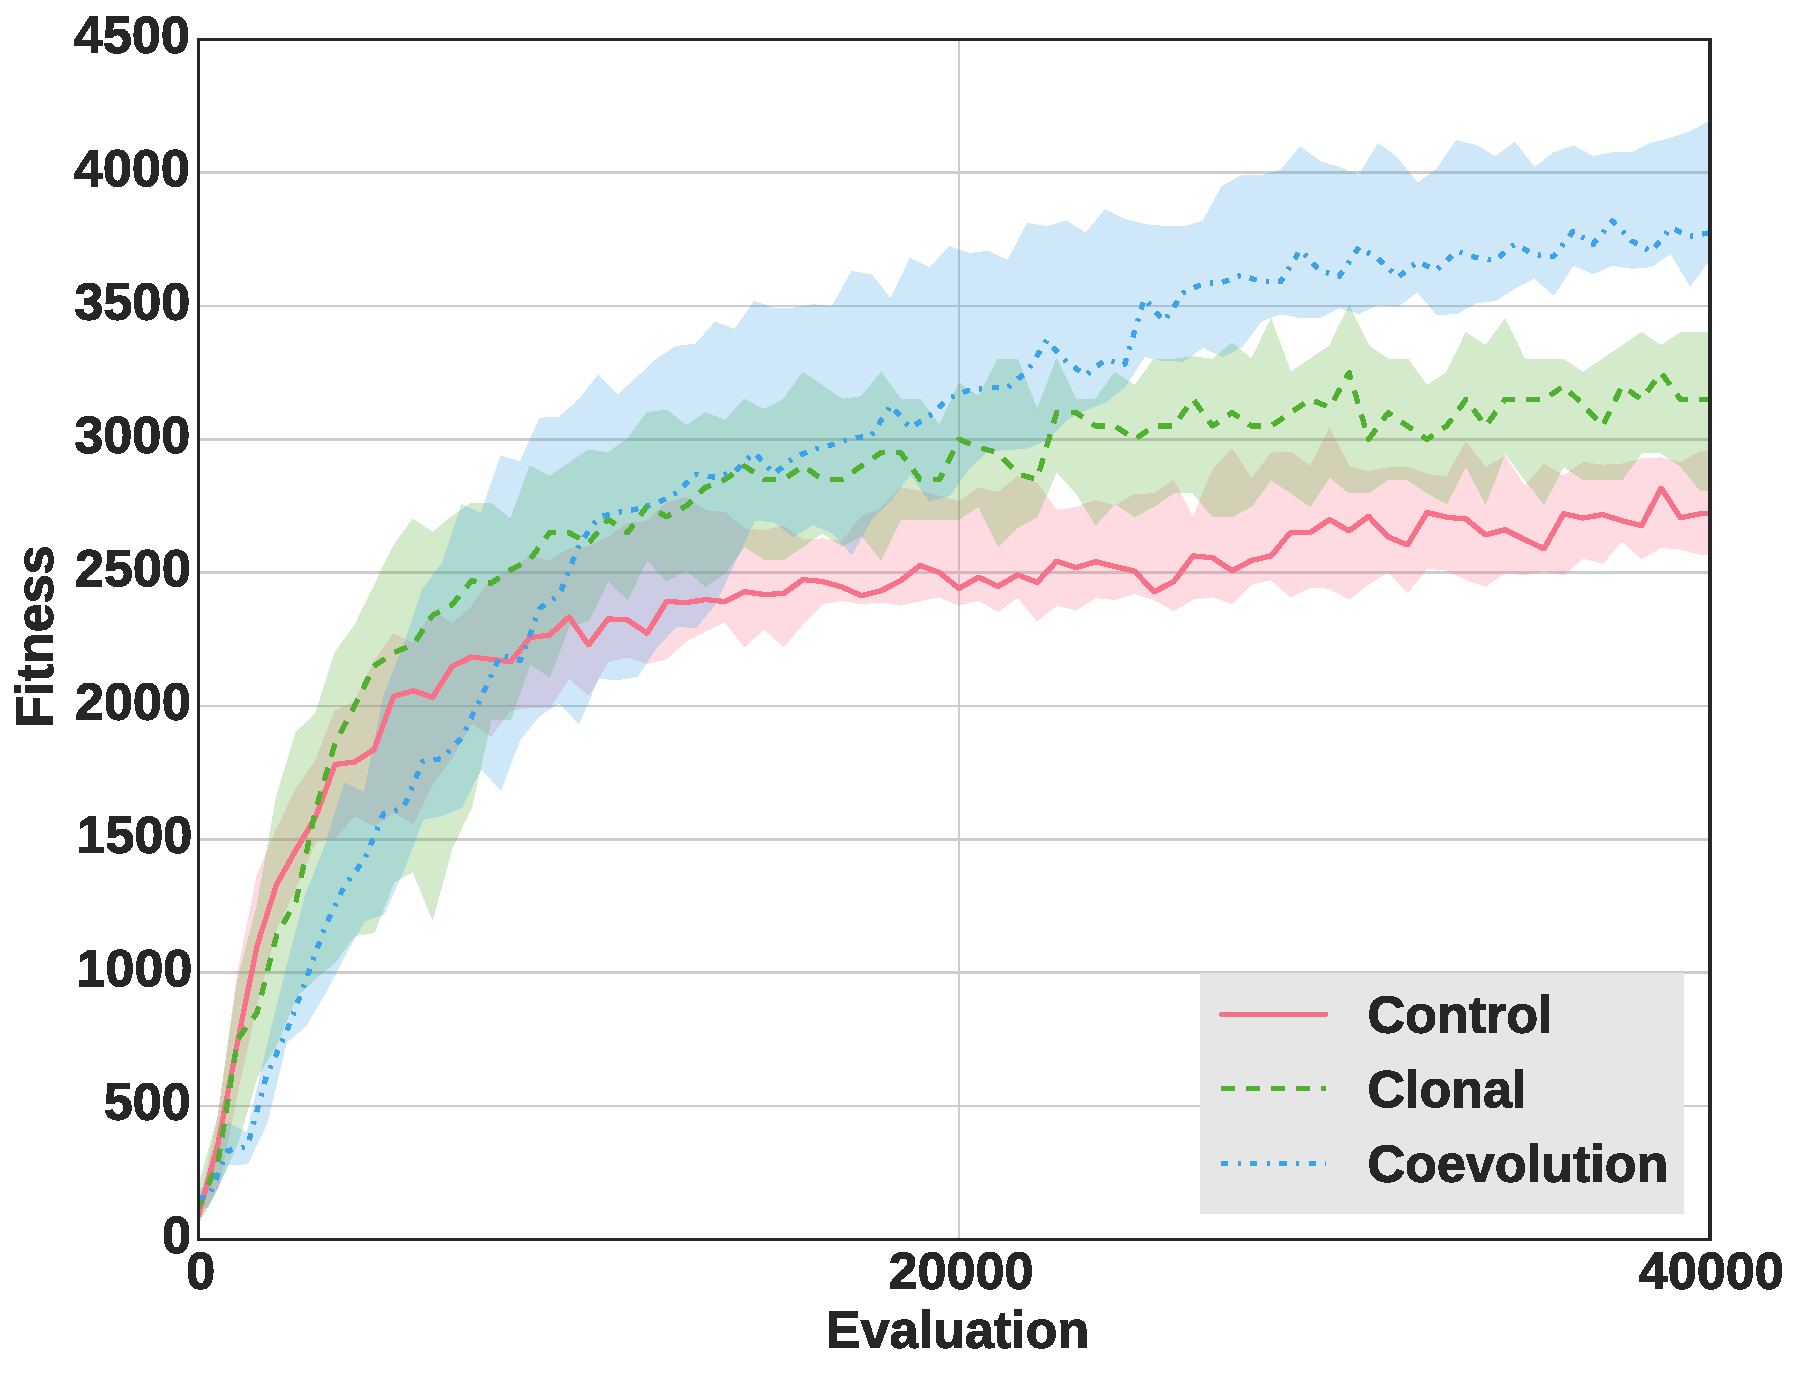
\includegraphics[scale = 0.40]{fig/ArticleRob1/fitnessHuntingStags.pdf}
        \caption{\textbf{Performance of the cooperative solutions.}
        Median fitness score of the best individuals in each of the runs where cooperation evolved for each setup over time. The fitness score of an individual is computed as the average reward the individual earned per trial by foraging targets. The colored areas around the medians represent the first and third quartiles.} 
        \label{fig:HuntingFitness}
      \end{center}
    \end{figure}

    However, cooperative individuals do not perform with the same \emph{efficiency} from one setup to another. We show in Figure~\ref{fig:HuntingFitness} the median fitness score of the best individuals in each independent run where cooperation evolved over time and for each setup. Fitness scores are significantly different in each setup with the best score obtained in the coevolution setup and the worst in the control setup (Mann-Whitney U-test on the fitness score of the best individuals at the last evaluation, {\em p}-value $< 0.001$).

    These differences in efficiency can be explained by looking at the nature of the cooperative behaviors evolved, which reveals two types of behaviors: \emph{turning} and \emph{leader/follower}.

    Individuals adopting the turning strategy turn around one another so that they always see the other individual as well as stay close to it (Figure~\ref{fig:behaviorHuntingTurning}). This allows the two individuals to approach simultaneously a same target and therefore forage it in a cooperative fashion. In this strategy, both individuals have a similar behavior and no role division is necessary for their successful cooperation.

    In comparison, individuals which evolve a leader/follower strategy adopt a differentiation between two roles: \emph{leader} and \emph{follower} (Figure~\ref{fig:behaviorHuntingLeadership}). The individual we call leader always goes first on a target whereas the follower always arrives second on the same target. We observe that the follower's behavior consists in staying close to the leader and always keeping it in front of itself. In comparison the leader shows a lesser interest in the presence of its follower and rarely checks on its position.


    \begin{figure}[h]
      \centering
        \begin{subfigure}[]
          {\label{fig:behaviorHuntingTurning} 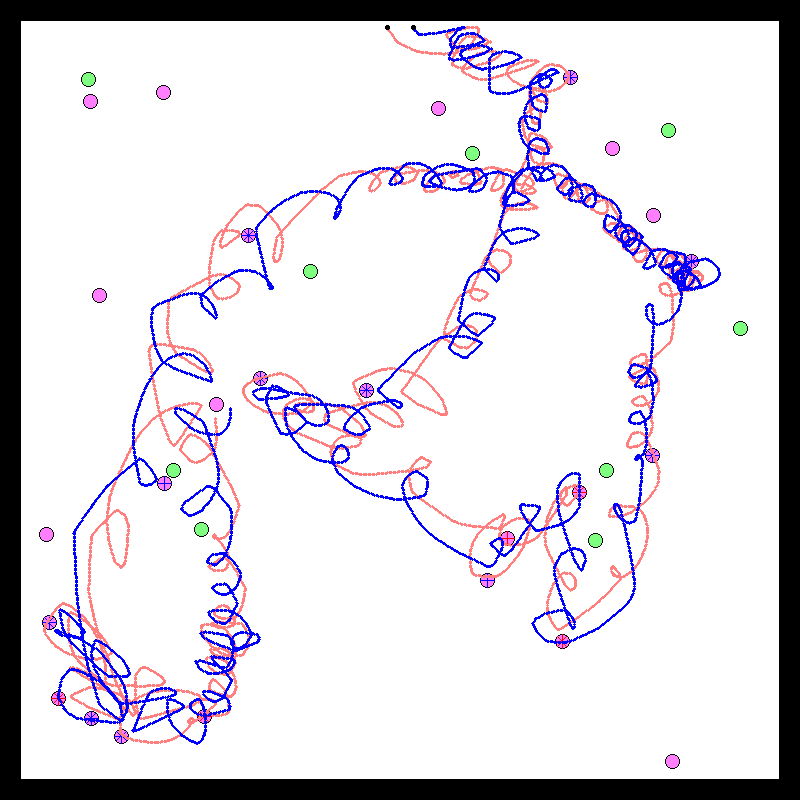
\includegraphics[scale=0.25]{fig/ArticleRob1/behaviorHuntingTurning.png}}
        \end{subfigure}~
        \begin{subfigure}[]
          {\label{fig:behaviorHuntingLeadership} 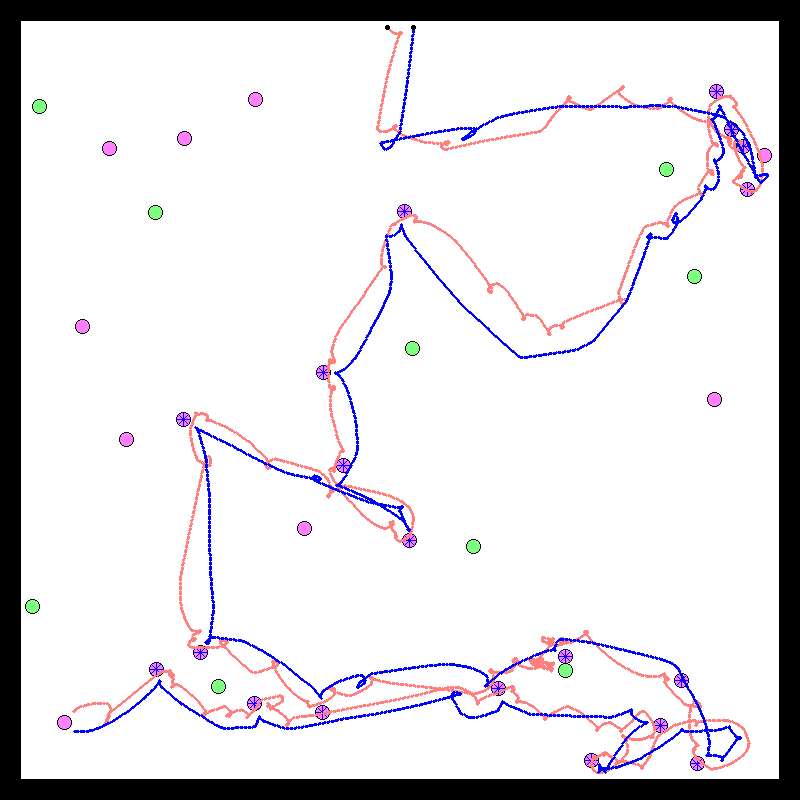
\includegraphics[scale=0.25]{fig/ArticleRob1/behaviorHuntingLeadership.png}}
        \end{subfigure}
        \caption{\textbf{Snapshots of the simulation after an entire trial in the foraging task.}
        The path of each robotic agent from their initial positions (black dots) is represented in red and blue. The green and purple discs represent the 18 targets in the environment. When a target is foraged by the two agents, a red cross (resp. blue) is drawn on the target if the red agent (resp. blue) arrived on it first. Each snapshot corresponds to a trial where agents adopted a different behavior: {\em (a)}~turning or {\em (b)}~leader/follower.}
        \label{fig:behaviorTracesHunting}
    \end{figure}


    Table~\ref{tab:ForagingBehaviors} shows the distribution of cooperative strategies for all three setups. Whereas the control and clonal setups always resulted in turning strategies (resp. 10/10 and 28/28), the coevolution setup always displayed the evolution of a leader/follower strategy (14). We observe that this latter strategy leads to more efficient cooperation. Indeed, individuals adopting the turning strategy are forced to check constantly on the other individual's position. Consequently, they cannot be as fast as individuals with a leader/follower strategy where they move to the target in a straight line under the leader's direction. Moreover, due to the random proximity of the targets, the turning strategy is prone to errors. Namely, they often get to another target than that of their partner whenever two targets are too close to each other.

    A possible explanation as to why no leader/follower strategy could evolve in the control and clonal setups may be because of the need to differentiate between the two roles. Indeed, there needs to be the existence of an asymmetry between the two individuals for this phenomenon to appear. With coevolved populations, this asymmetry is deliberately created by the separation between the two populations. Indeed, we observe that one population exclusively contains leaders while the other exclusively contains followers. 

    The two other setups fail to evolve heterogeneous behaviors. In the control setup, this may be due to the evolutionary algorithm used, especially with elistism enforcing the homogenization of the population throughout the course of evolution (as hinted in the Methods Section). Then, the clonal setup introduces yet another challenge as switching to a particular role can only be done during evaluation as both individuals are by definition genetically similar.

    \begin{table}[h]
      \center{
        \begin{tabular}{lccc}
          \hline
          \textbf{Setting} & \textbf{\# Leader/Follower} & \textbf{\# Turning} & \textbf{Total}\\ 
           & \textbf{Strategy} & \textbf{Strategy} & \\ 
          \hline
          \textit{Control} & 0 & 10 & \textbf{10}\\
          \textit{Clonal} & 0 & 28 & \textbf{28}\\
          \textit{Coevolution} & 14 & 0 & \textbf{14}\\
          \hline
        \end{tabular}
      }
      \caption{\textbf{Evolution of a cooperative strategy.}
      Repartition of the different strategies evolved in each of the runs where cooperation evolved for each setup in the foraging task. We indicate in each cell the number of simulations where a particular strategy evolved.}
      \label{tab:ForagingBehaviors}
    \end{table}

\section{Going Beyond the Evolvability vs. Efficiency Tradeoff using Incremental Evolution}

  The previous section revealed a tradeoff between evolvability and efficiency. In the clonal setup, cooperation evolves more often than with other setups. However, the coevolution setup yields cooperative behaviors which are more efficient, with paired individuals displaying asymmetrical behaviors.

  In this section, we address the following question: is it possible to benefit from both evolvability \textit{and} efficiency with the clonal and/or the coevolution setups? In other words, we explore (1) whether the clonal setup can be used to evolve pairs with heterogeneous behaviors, and (2) whether the coevolution setup can be improved in terms of number of runs where cooperation evolved.

  In order to address this question, we use incremental evolution, a rather common method in evolutionary robotics for solving challenging problems~\parencite{Dorigo1994,Saksida1997,Bongard2008,Doncieux2013}. The main principle is to ease the learning of a complex task by splitting it into simpler sub-tasks~\parencite{Perkins1996}.

  In the following, we introce an additional task, the \textit{waypoints crossing} task, which requires the evolution of coordination behaviors, and is simpler to address than the preous task. Individuals evolved in this first task are then used as starting point for the original task described earlier, hoping that cooperative behavior will be \emph{recycled} from the first task to the second task.
  
  \subsection{Waypoints Crossing Task}  

    We consider a task where robotic agents have to cross randomly positioned waypoints. As such, these round waypoints do not act as obstacles and have a diameter of 30 units. As soon as an agent goes through a waypoint, it can not be seen by this agent anymore. All 18 waypoints have the same color and can be crossed in any order. The fitness score (\(F\)) of each individual is defined as the average longest sequence of waypoints shared by both agents per trial:

    \[
    F = \frac{1}{N*M} \sum_{i=1}^{N} \sum_{j=1}^{M} l_{max_{ij}}
    \]

    Where \(N\) is the number of individuals encountered ($5$ in the control and coevolution setups, $1$ in the clonal setup), \(M\) the number of trials ($5$) and \(l_{max_{ij}}\) the longest sequence of waypoints shared by both individuals at trial \(j\) with individual \(i\).

    This implies that the two individuals are rewarded when crossing waypoints in the same order as well as maximizing the number of waypoints crossed. Each evaluation lasted $10000$ simulation steps and $60$ independent runs were conducted for each experimental setup, each one lasting $40000$ evaluations.

    \begin{figure}[h]
      \begin{center}
        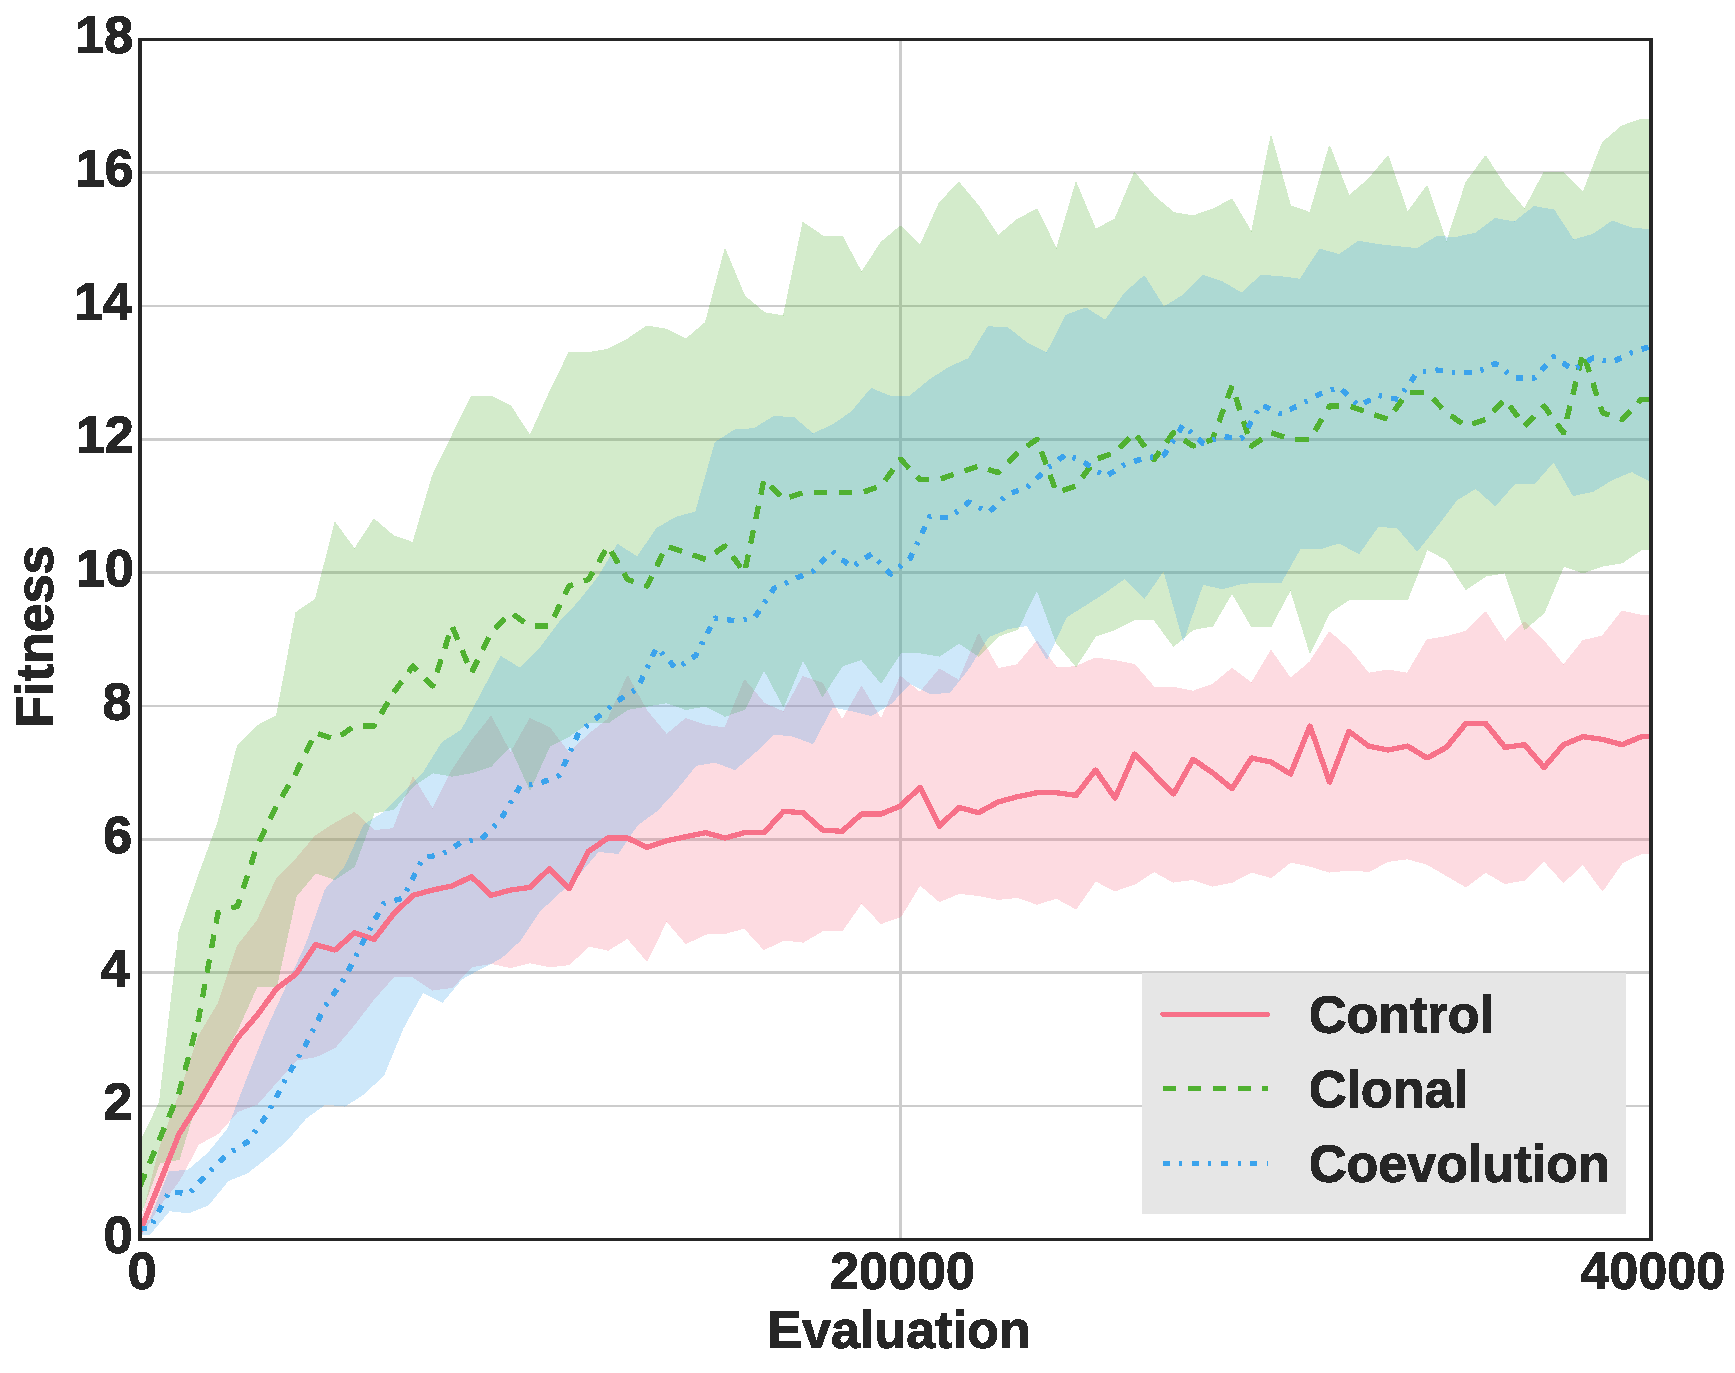
\includegraphics[scale = 0.4]{fig/ArticleRob1/fitnessWaypoints.pdf}
        \caption{\textbf{Performance of the cooperative solutions.}
        Median fitness score of the best individuals in each of the 60 independent runs and for each setup over time. Fitness score is computed as the average longest sequence of waypoints shared by both agents per trial. The colored areas around the medians represent the first and third quartiles.}
        \label{fig:WaypointsFitness}
      \end{center}
    \end{figure}

    All simulations showed an increase in fitness score for each of the three setups (cf. Figure~\ref{fig:WaypointsFitness}). This was expected as this task does not represent a particular challenge for the individuals: it simply needs the evolution of a successful coordination strategy. However, whereas the coevolution and clonal setups performed equally, they both surpassed the performance of individuals from the control setup (Mann-Whitney, {\em p}-value $< 0.001$).

    As with the previous foraging task, we can hypothesize that these differences in fitness scores are due to differences in the behaviors evolved. Table~\ref{tab:WaypointsBehaviors} gives a classification of the cooperative behaviors for each setup. They are similar to those in the previous task with the addition of a third rare strategy: the \emph{wall-following} strategy (which is regrouped in ``Other''). Wall-followers simply follow the walls around the arena and cross any waypoints close to the wall they are adjacent to. As such, this is a far less efficient strategy than the two others. 


    \begin{table}[h]
      \center{
        \begin{tabular}{lcccc}
          \hline
          \textbf{Setting} & \textbf{\# Lead.} & \textbf{\# Turn.} & \textbf{\# Other} & \textbf{Total}\\ 
           % & \textbf{Strategy} & \textbf{Strategy} & \textbf{Strategy} & \\ 
          \hline
          \textit{Control} & 19 & 37 & 4 & \textbf{60}\\
          \textit{Clonal} & 23 & 31 & 6 & \textbf{60}\\
          \textit{Coevolution} & 59 & 1 & 0 & \textbf{60}\\
          \hline
        \end{tabular}
      }
      \caption{\textbf{Cooperative strategies evolved.}
      Repartition of the different strategies evolved in each of the 60 independent runs for each setup in the waypoints task. We indicate in each cell the number of simulations where a particular strategy evolved: \emph{Leader/follower} (Lead.), \emph{Turning} (Turn.) or \emph{Other}. ``Other'' regroups wall-following strategies or simulations where no recognizable strategy evolved.}
      \label{tab:WaypointsBehaviors}
    \end{table}

    \begin{figure}[h]
      \centering
        \begin{subfigure}[]
          {\label{fig:leadershipControl} 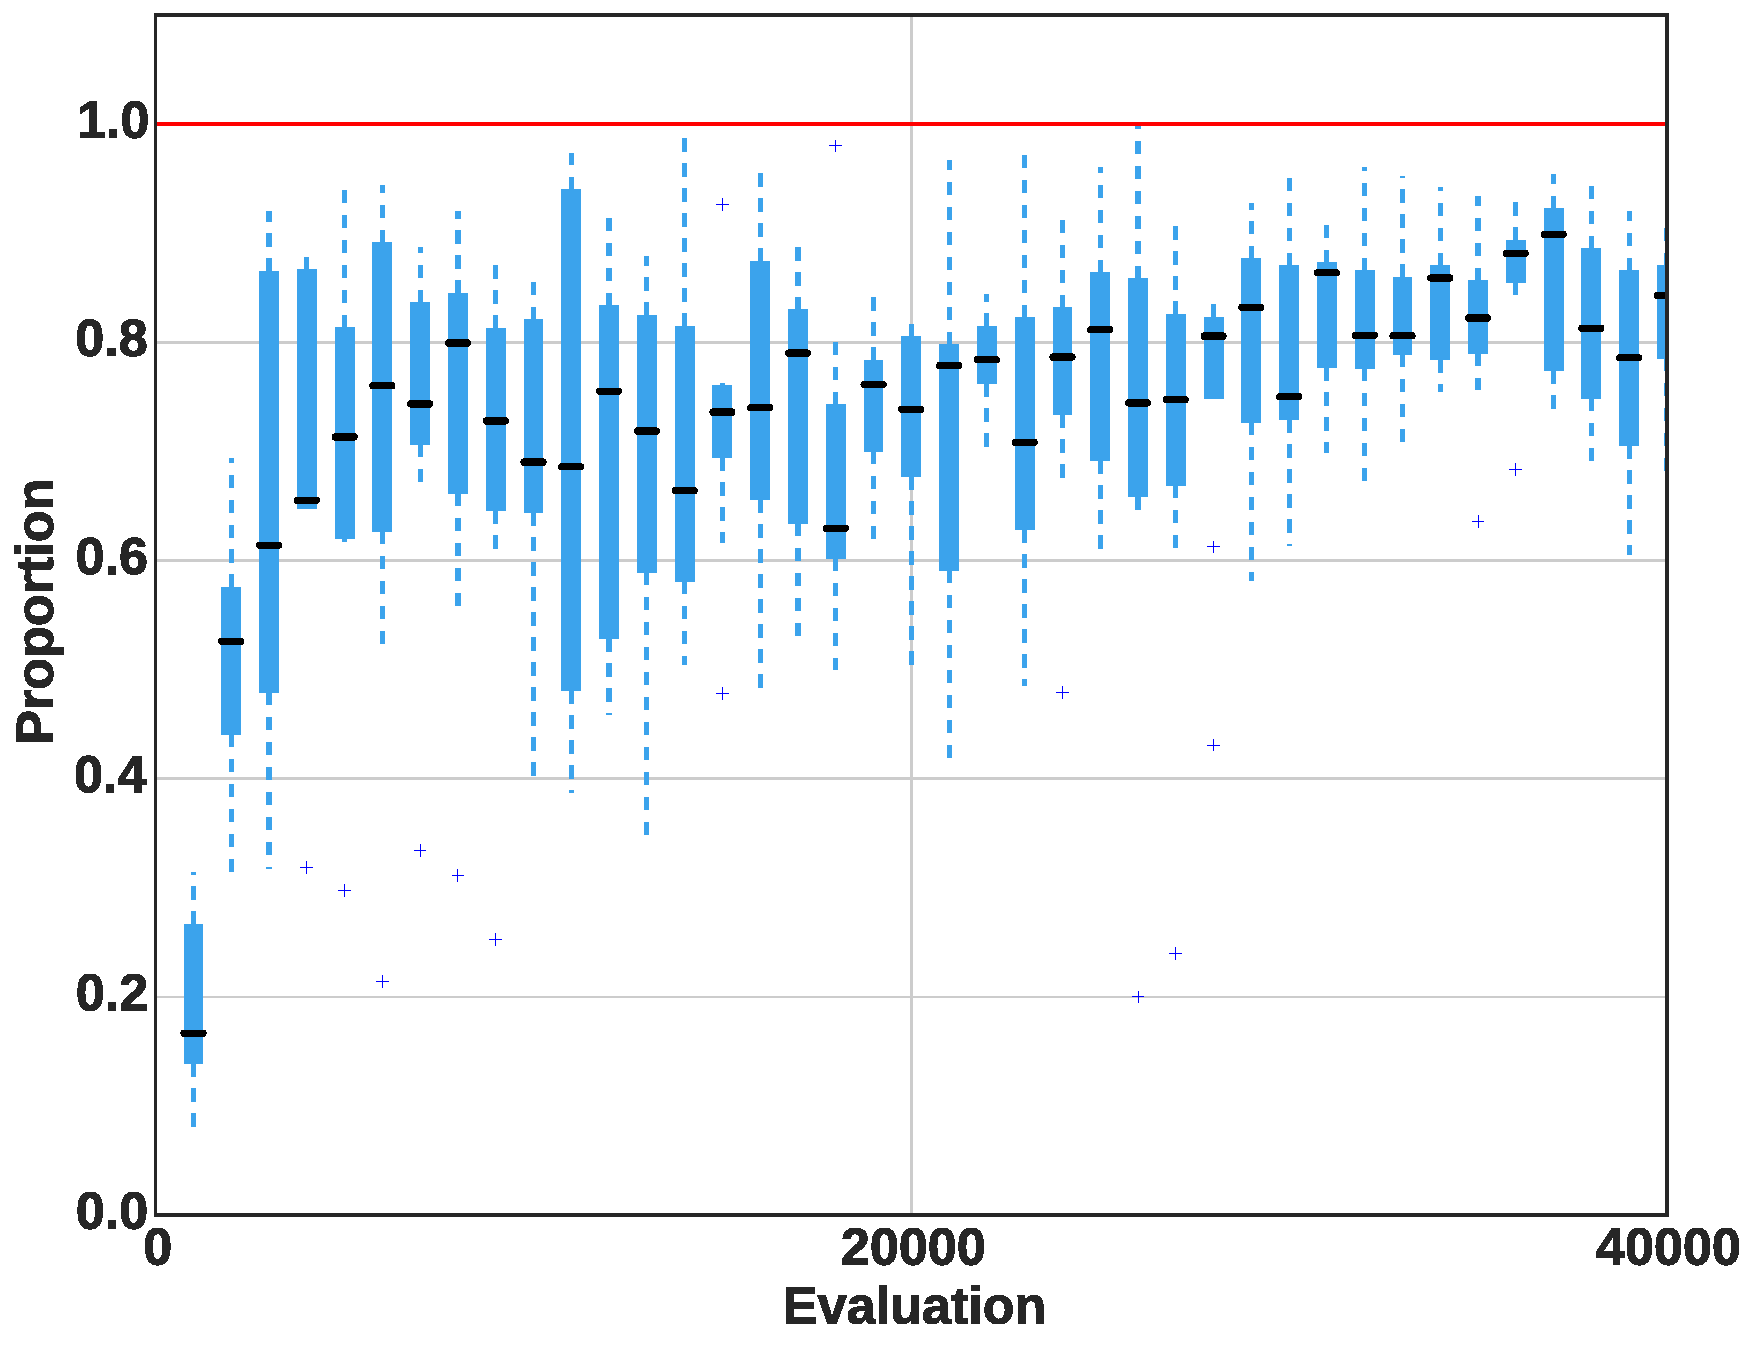
\includegraphics[scale=0.25]{fig/ArticleRob1/proportionLeadershipControl.pdf}}
        \end{subfigure}
        \begin{subfigure}[]
          {\label{fig:leadershipClonal} 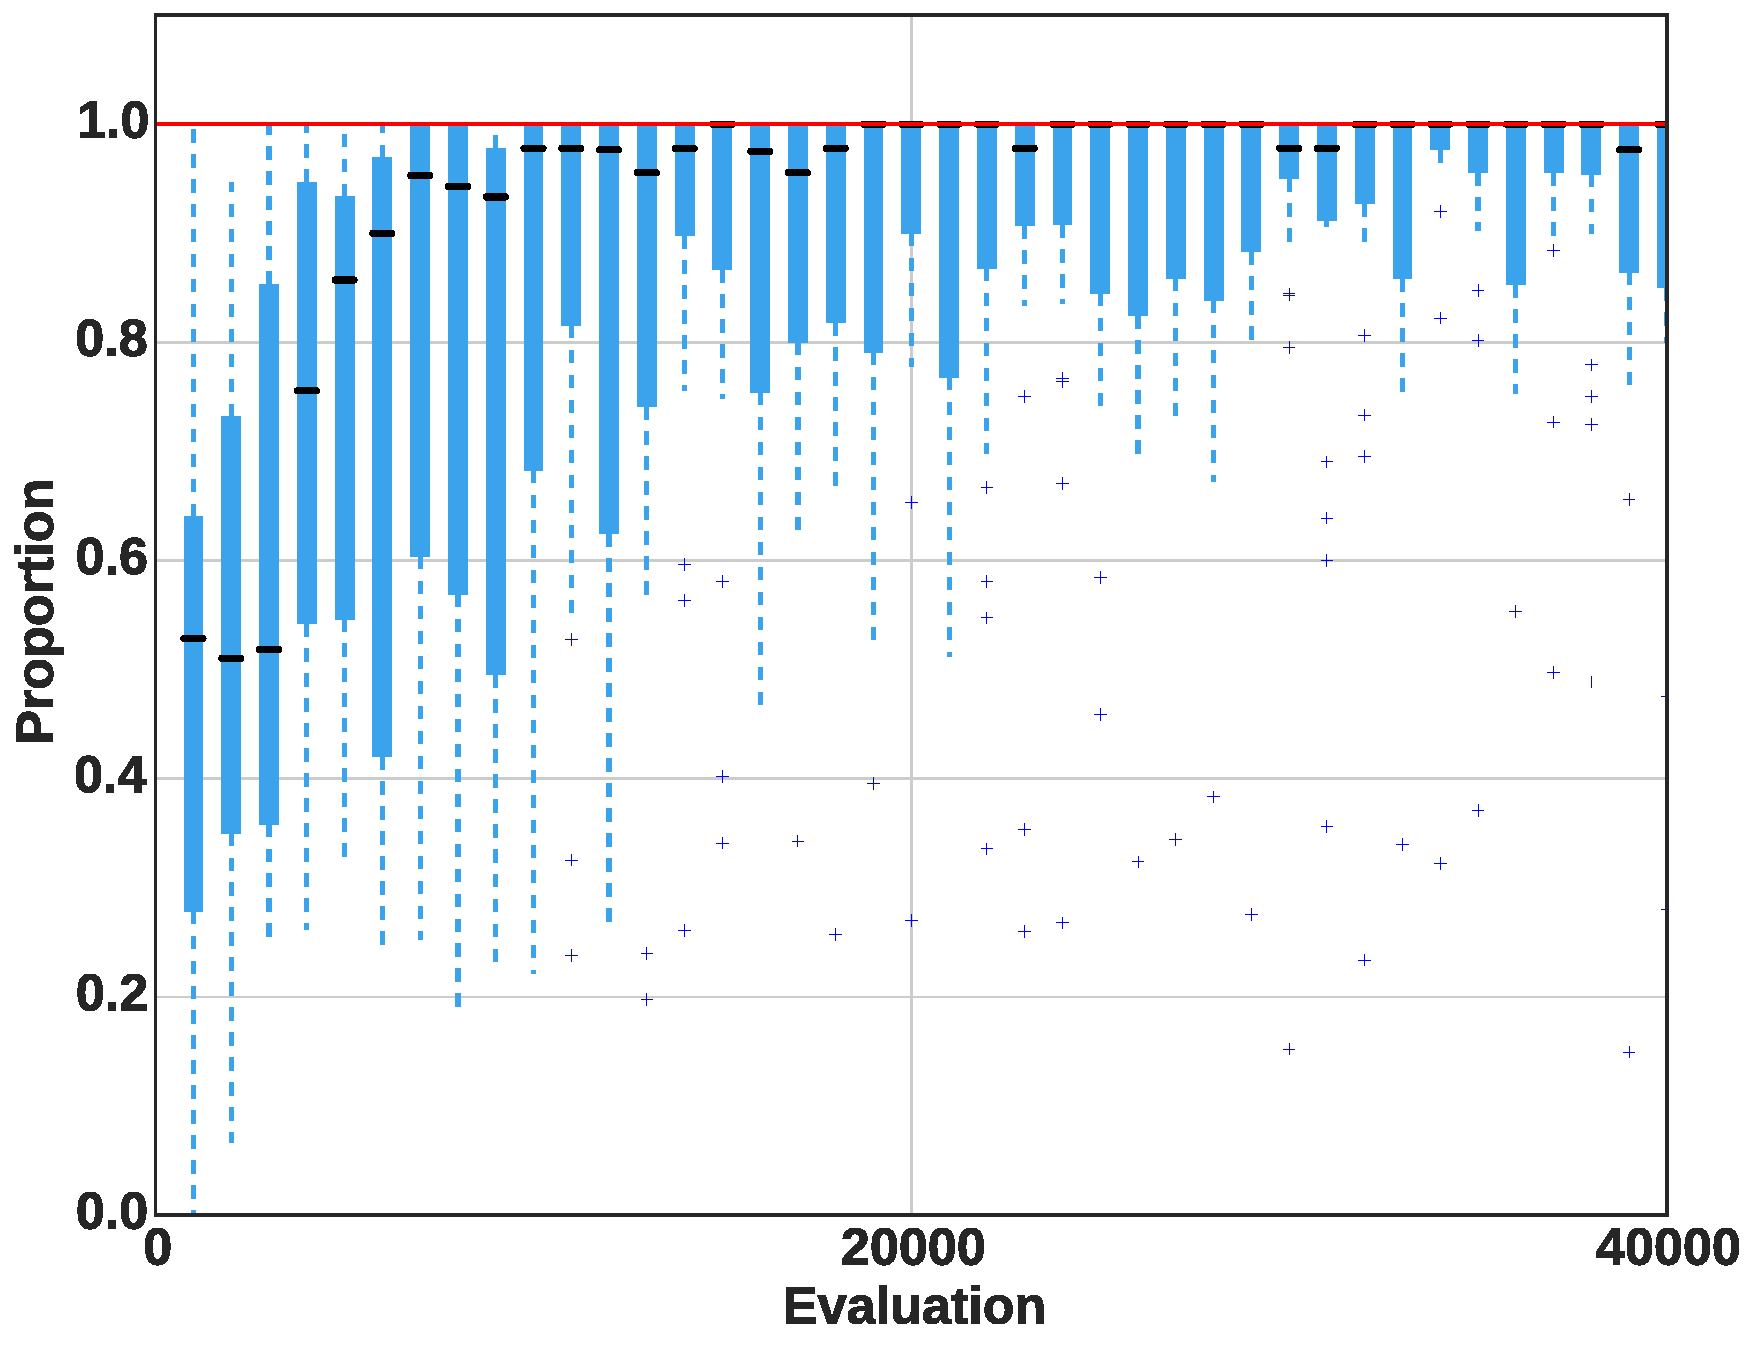
\includegraphics[scale=0.25]{fig/ArticleRob1/proportionLeadershipClonal.pdf}}
        \end{subfigure}
        \begin{subfigure}[]
          {\label{fig:leadershipCoevo} 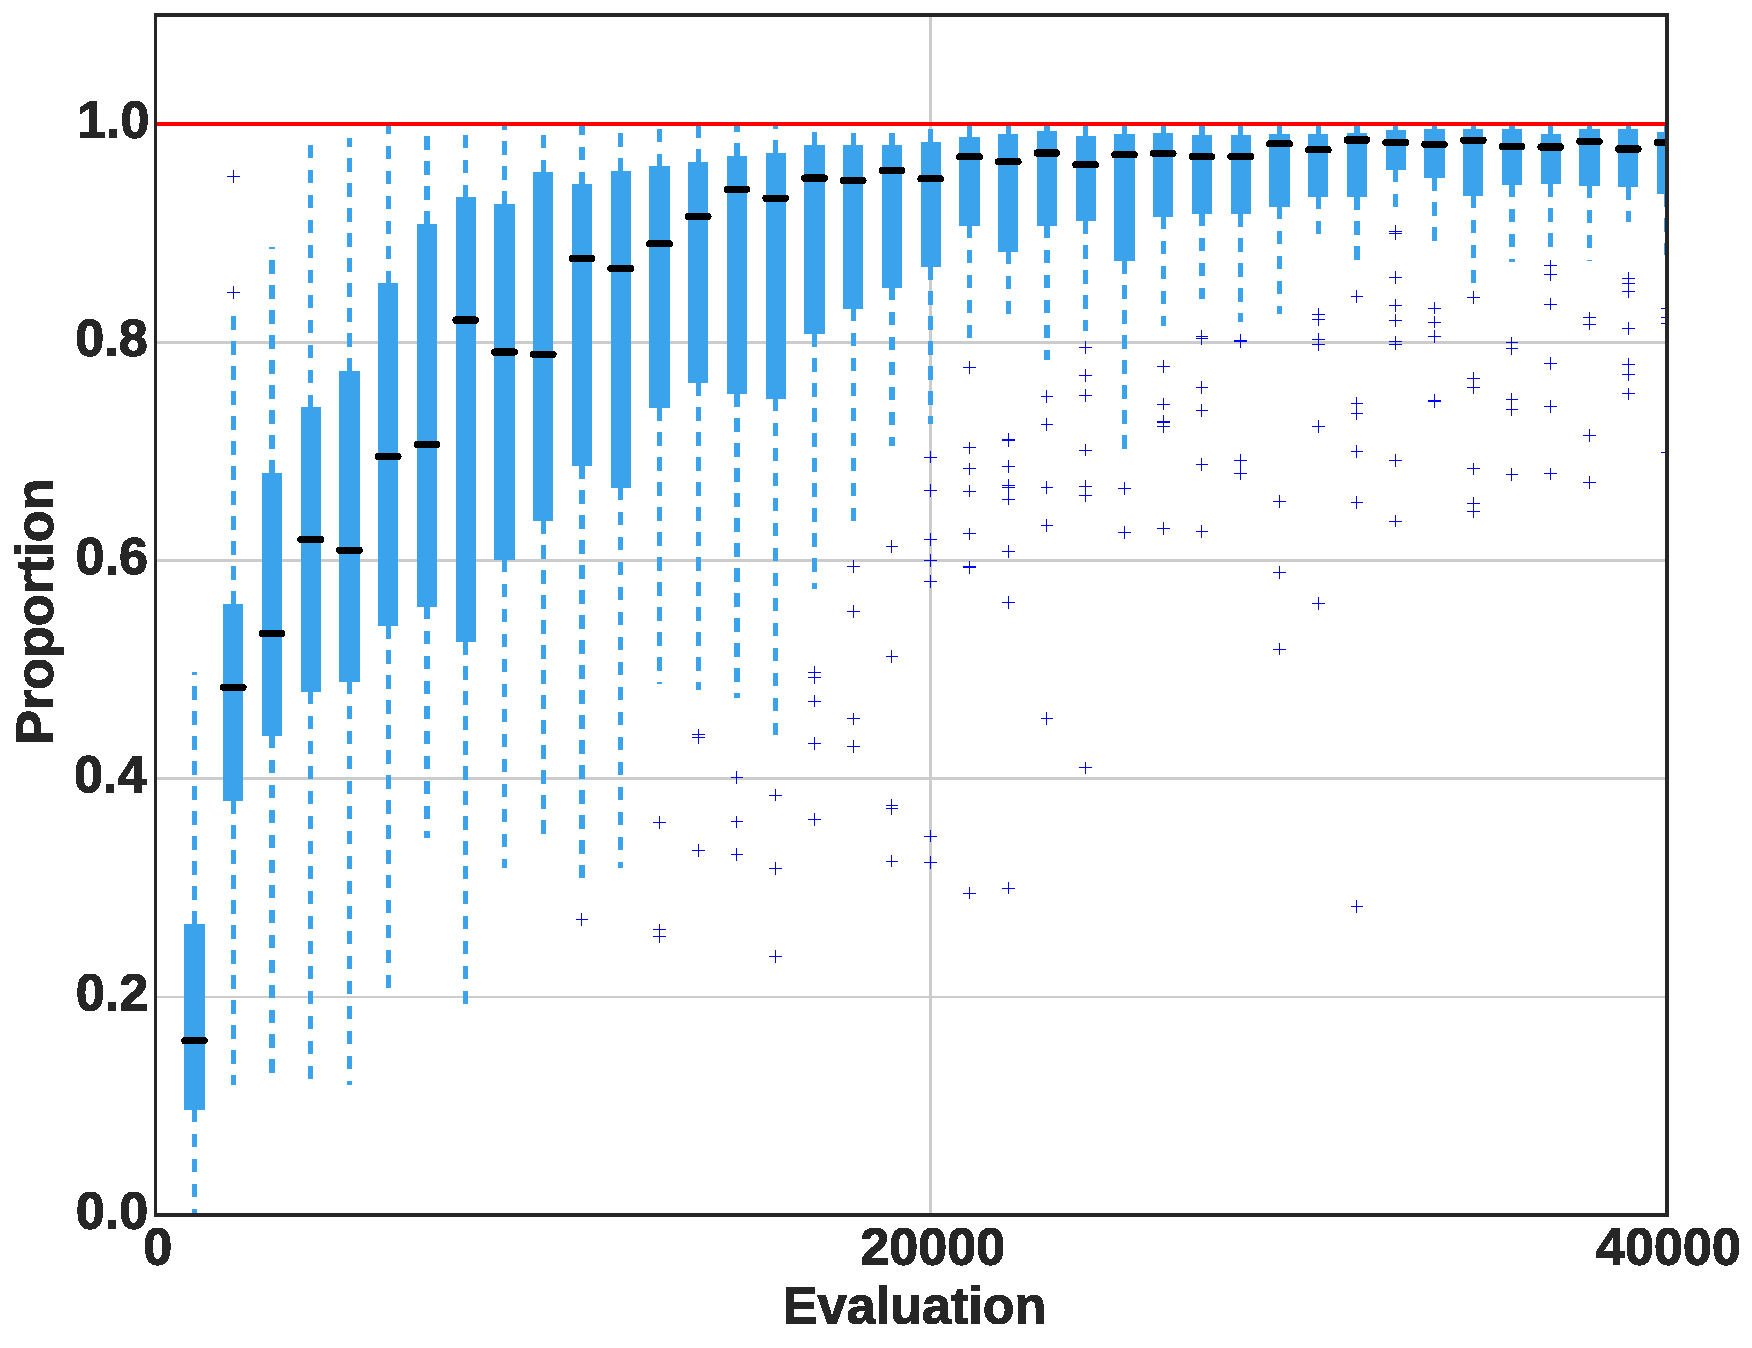
\includegraphics[scale=0.25]{fig/ArticleRob1/proportionLeadershipCoevo.pdf}}
        \end{subfigure}
        \caption{\textbf{Proportion of leadership.}
        Boxplots of the proportion of leadership over time for the best individuals in each runs where the proportion at the last evaluation was greater than 0.75 in the {\em (a)}~control, {\em (b)}~clonal or {\em (c)}~coevolution setup. This value represents the proportion of waypoints crossed by both individuals for which the leader arrived first.}
        \label{fig:WaypointsLeadership}
    \end{figure}

    In the coevolution setup, nearly all runs (59/60) evolved a leader/follower strategy. Interestingly, although fitness scores in the clonal and control setups are significantly different, this behavior evolved in roughly one third of the runs for both setups. To explain the difference in fitness scores, we must take into account the quality of the leader/follower strategy in each setup. We measure the proportion of leadership in each interaction, which is computed as the proportion of waypoints crossed by both individuals for which the leader arrived first. Figure~\ref{fig:WaypointsLeadership} displays the boxplots of the proportion of leadership for the best individuals in each setup and only for the simulations where a successful leader/follower strategy evolved (a minimal threshold of 0.75 is chosen to consider only the best performing runs). We show that the proportion of leadership is greater in the clonal and coevolution setups than in the control one (Mann-Whitney, {\em p}-value $< 0.005$). These differences means that the individuals are more efficient in their leader/follower strategy in the clonal and coevolution settings than in the control one. This explains the differences in fitness scores observed in Figure~\ref{fig:WaypointsFitness}.

    Interestingly, whereas in the foraging task no leader/follower strategy could evolve in the control and clonal setups, this strategy did evolve in one third of the simulations for this task. This could mean that these individuals use information in the environment to adopt one role or the other. Indeed, we observe that this is achieved by exploiting the differences in the initial starting positions, with one individual on the left and the other on the right. They both turn to the same direction (left or right, depending on the runs) at the beginning of the simulation which results in one individual (the leader) turning its back to the other, while the second individual (the follower) looking at its partner. 


  \subsection{Recycling Cooperative Behaviors in the Foraging Task}

    Coming back to the initial foraging task, we perform the exact same experiment described at the beginning of this paper, with one notable exception: the initial population is initialized with genomes evolved for solving the waypoint task. This implies that coordination is possible starting from the very first generation of each setup. Given that we have already shown that such coordination is a desirable feature, the question is: will it be possible to retain cooperative behaviors in order to solve the foraging task?

    \begin{table}[h]
      \center{
        \begin{tabular}{lcccc}
          \hline
          \multirow{2}{*}{\textbf{Setting}} & \multicolumn{2}{c}{\textbf{\# Coop.}} & \multirow{2}{*}{\textbf{\# Solitary}} & \multirow{2}{*}{\textbf{Total}}\\ 
          \cline{2-3}
           & \textbf{\# Lead.} & \textbf{\# Turn.} & & \\ 
          \hline
          \textit{Control} & 0 & 20 & 40 & \textbf{60}\\
          \textit{Clonal} & 0 & 24 & 36 & \textbf{60}\\
          \textit{Coevolution} & 28 & 0 & 32 & \textbf{60}\\
          \hline
        \end{tabular}
      }
      \caption{\textbf{Evolution of a cooperative strategy.}
      Proportion of the 60 independent simulations where the best individual evolved a cooperative strategy (collecting purple targets) or a solitary strategy (collecting green targets) for each setup in the foraging task when individuals are previously evolved in the waypoints task. In addition, the repartition of the different strategies is indicated when cooperation evolved: \emph{Leader/Follower} (Lead.) or \emph{Turning} (Turn.).}
      \label{tab:RecyclingCoopBehaviors}
    \end{table}

    Table~\ref{tab:RecyclingCoopBehaviors} gives the results in terms of evolved behaviors from the $60$ independent runs for each setup. 
    The coevolution setup evolves cooperation slightly more often (28/60) than both the control (20/60) and the clonal (24/60) setups. 
    A first remark is that the number of occurences of cooperation for the coevolution and control setups have actually doubled compared to previous results without incremental evolution (see Table~\ref{tab:ForagingCoop}). This is not the case for the clonal setup, which does not appear to benefit from incremental evolution. 

    A second remark is that cooperation in the coevolution setup systematically corresponds to a leader/follower strategy, which is \textit{never} the case with the two other setups. This has a significant, though expected, impact on fitness scores, as shown in Figure~\ref{fig:RecyclingFitness}. Cooperation evolved with the coevolution setup leads to significantly greater fitness scores (Mann-Whitney, {\em p}-value $<0.001$). 

    Results from this experiment make it possible to revise our initial statement. Using pre-trained individuals strongly benefits the coevolution setup in terms of evolvability. But this is not the case with the clonal setup, for which using pre-trained individuals improves neither evolvability nor efficiency. Therefore, we may face a tradeoff which does not concern evolvability and efficiency, but one that implies computational cost: the coevolution setup outperforms the clonal setup on both evolvability and efficiency \textit{at the cost of additional computational effort}.

    The control and clonal setups completely failed to maintain a leader/follower strategy, even though such strategy originally evolved. An explanation is provided by considering the difference between the waypoints task, where leader/follower evolved, and the current foraging task. In the waypoints task, symmetry breaking could be achieved at the beginning of the evaluation (as explained earlier), and could be retained afterwards as the follower was always behind the leader. However, the current foraging setup requires that the two robots display the same behavior to cooperatively collect a target (ie. both robots have to touch the target), which implies that leader/follower roles are lost, as they depend on the relative position of robots with one another. 


    \begin{figure}[h]
      \begin{center}
        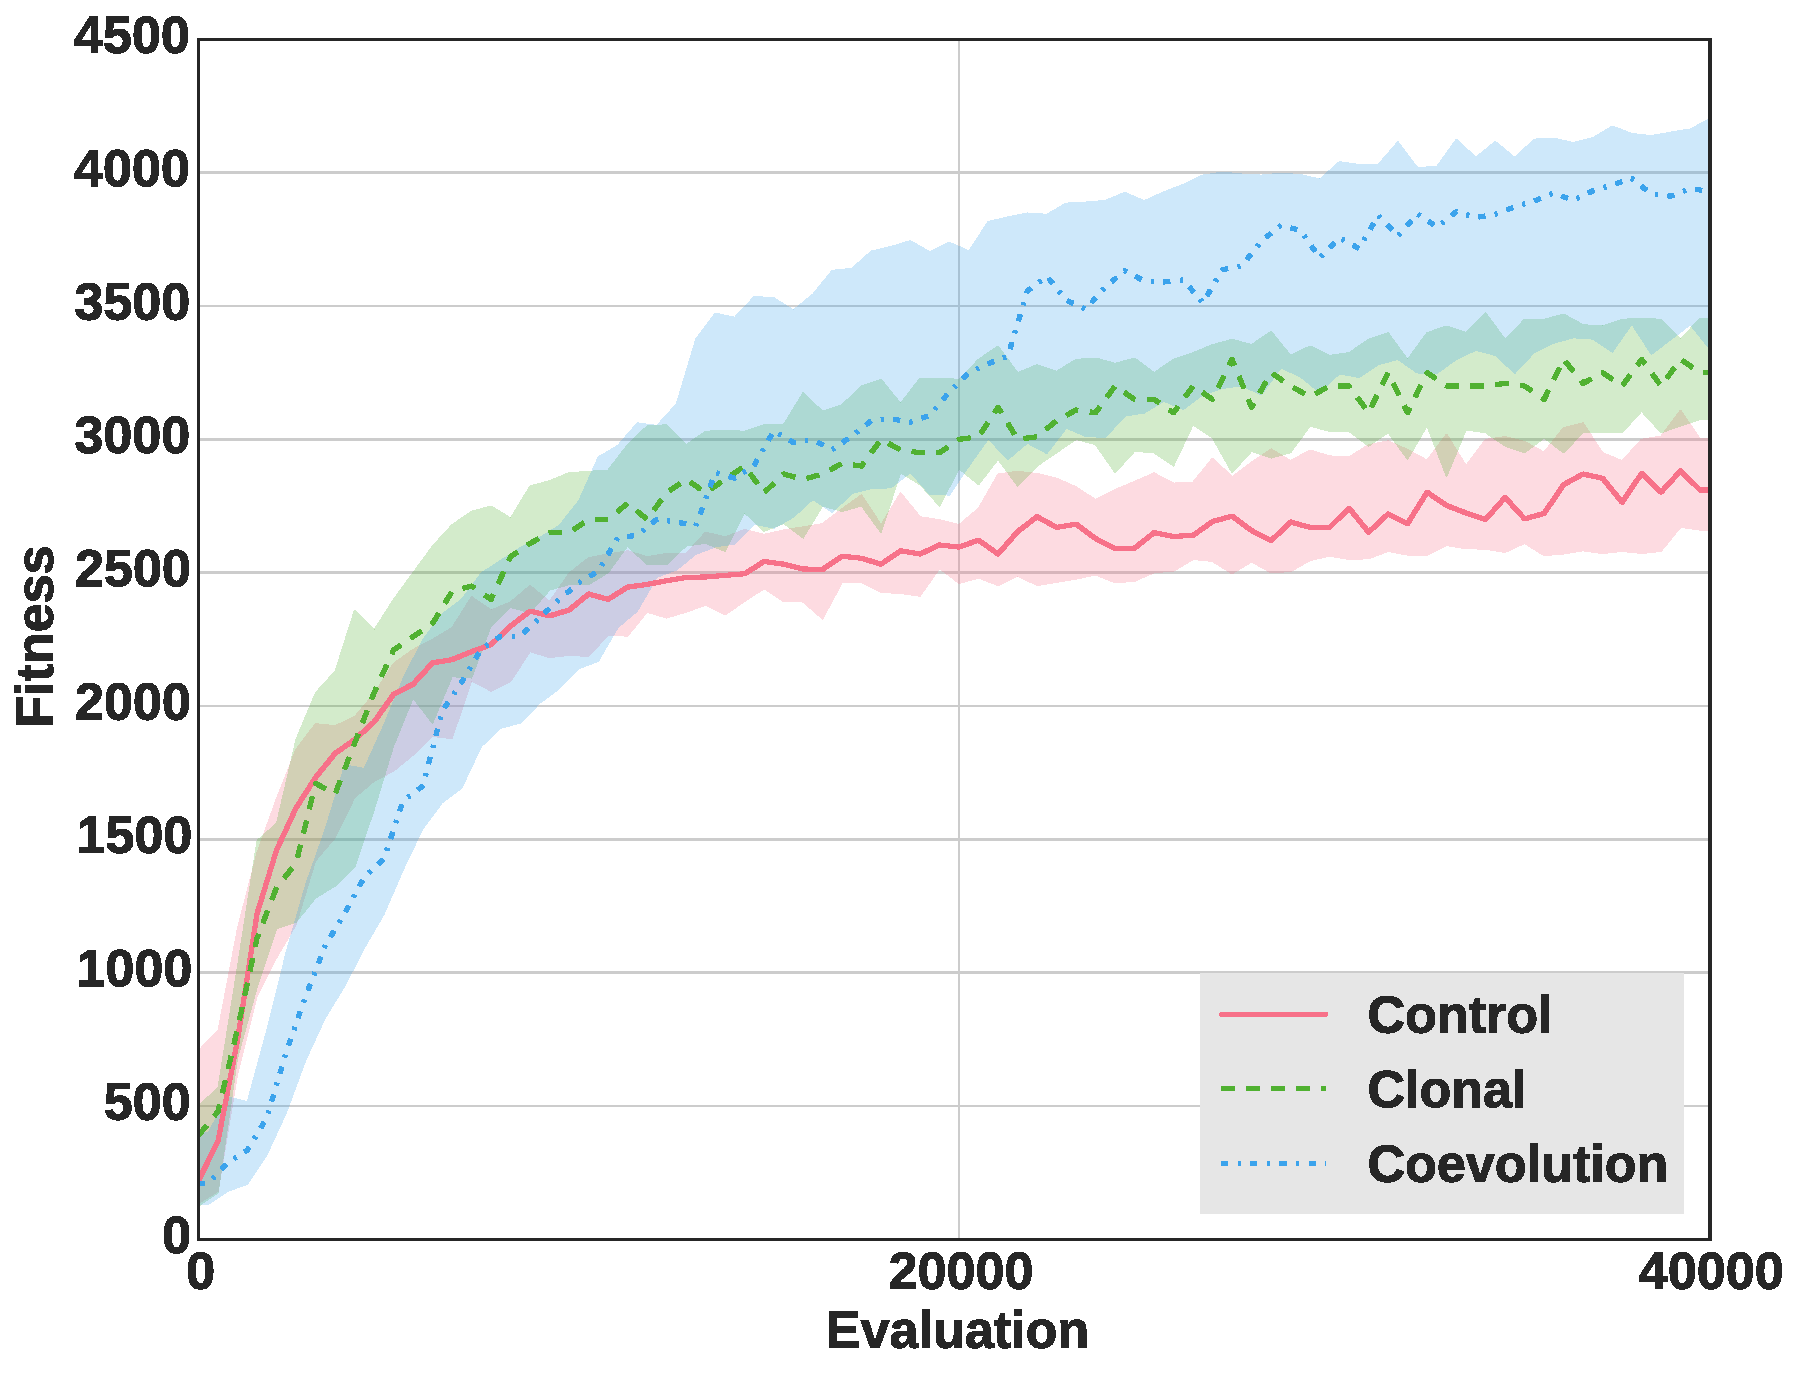
\includegraphics[scale = 0.4]{fig/ArticleRob1/fitnessRecyclingStags.pdf}
        \caption{\textbf{Performance of the cooperative solutions.}
        Median fitness score of the best individuals in each of the runs where cooperation evolved for each setup over time. The fitness score of an individual is computed as the average reward the individual earned per trial by foraging targets. The colored areas around the medians represent the first and third quartiles.}
        \label{fig:RecyclingFitness}
        \end{center}
    \end{figure}

\section{Discussion and Conclusion}

  In this paper, we considered several approaches for the evolution of cooperation in evolutionary robotics: a clonal approach, where all individuals in a group share the same genome, and a non-clonal approach, where individuals are independent from one another, but may share a common interest in cooperating. 

  We first showed that there exists a tradeoff between evolvability and efficiency. On the one hand, the clonal approach evolves cooperative behaviors on a more frequent basis than with the other approach. On the other hand, the non-clonal approach, which is implemented using a coevolution setup, results in more efficient behaviors in terms of pure performance whenever cooperation evolved. The non-clonal approach actually enables the evolution of asymmetric behaviors, such as a leader/follower strategy.

  We then used incremental evolution to evolve coordination behaviors using a simpler task in order to overcome this tradeoff and improve both evolvability and efficiency in each setup. We showed that while no improvement was observed in the clonal setup on either criteria, the outcome is very different for the coevolution setup: the probability of evolving cooperation actually increases, and the evolved cooperative solutions remain the most efficient.
 
  This work raises several questions. Firstly, heterogeneous behaviors were obtained with coevolution, a rather radical way to enable asymmetrical behaviors during cooperation. However, the waypoints task revealed that breaking symmetry can also be done with identical individuals using environmental feedback, even though such cooperation is difficult to obtain. As a consequence, we intend to investigate the evolution of cooperation with heterogeneous behavior without resorting to coevolution. In particular, we will study how more elaborated neural architectures (e.g. using plasticity) can switch to a particular persistant regime depending on environmental cues available at the beginning of the evaluation.

  Secondly, incremental evolution requires an added computational cost in order to increase evolvability in the non-clonal approach. However, it may be possible to avoid this extra cost by considering other evolutionary methods. In particular, we intend to explore how a multiobjective approach which considers both performance and \emph{diversity} could improve the optimization process~\parencite{Lehman2008, Doncieux2014}. Though this approach looks promising, it is not clear yet how diversity should be implemented in the context of cooperative problem solving.

\chapter{The Evolution of Specialization through Genotypic Polymorphism}
\label{chapter:C2_article2}

\setcounter{secnumdepth}{0}
\setcounter{minitocdepth}{1}
\minitoc[n] % minitoc without title

We now investigate the evolution of division of labour between heterogeneous robots via genotypic polymorphism. Results are presented as a published article in an international conference:

\begin{quote}
  \fullcite{Bernard2016b}
\end{quote}


In the previous Chapter we showed that it could be beneficial to consider the quality of cooperative behaviours in addition to the probability to evolve cooperation. In particular, we revealed that a particular heterogeneous approach, cooperative coevolution, led to the emergence of a more efficient coordination behaviour: leader/follower. This behaviour entails the evolution of task specialisation (or division of labour). Here we focus on the evolution of a leader/follower strategy in a single population of individuals. 

Because in evolutionary robotics cooperation is often evolved among homogeneous robots, this means that in order to achieve division of labour, individuals must be capable to adapt their phenotype during their lifetime. In consequence, specialisation relies on phenotypical plasticity or environmental cues. Here we are interested in evolving specialisation without additional mechanisms. This means that we want to achieve division of labour at the level of the population. In consequence, we want to investigate the maintenance of several different genotypes encoding for different roles in a single population, i.e. genotypic polymorphism. In particular, we focus on the impact of selection strategies on evolving genotypic polymorphism.

To that end, we use a simpler foraging task than the one presented in Chapter~\ref{chapter:C2_article1}. Two genetically different individuals are placed in arena where they can collect a single type of targets. This target is more rewarding when collected in a cooperative manner. This means that evolving cooperation is easy (we are not interested in the issue of evolving cooperation here) and that the task if favored by the evolution of efficient coordination strategies. As we showed in the previous Chapter, two different cooperative strategies can evolve in this setting. On the one hand, there is the turner strategy, where both individuals adopt the same behaviour to coordinate. Therefore this is a generalist behaviour. On the other hand, they can also evolve specialist behaviours and adopt a leader/follower strategy. We are interested on studying the evolutionary differences of two selection schemes: (1) a \((\mu + \lambda)\)-ES (elitist) selection strategy and (2) fitness-proportionate selection. We also study the impact of varying population size.

We reveal that specialisation is nearly impossible to evolve under an elitist selection strategy. Indeed, in only one replication under high population size do we observe the presence of specialists in the population at the end of evolution. Surprisingly however, specialists do appear in multiple replications but are never maintained. Even when the population is initially seeded with specialists, similar results are observed. In comparison, while specialists are nearly never bootstrapped under fitness-proportionate selection, they are easily maintained throughout evolution (especially when starting with a population of specialists). We thus reveal that evolving genotypic polymorphism is hindered by the challenge of both bootstrapping and maintaining specialists in the population and that none of these two classical selection schemes are suitable to that end.

We then use computational analyses to have a deeper understanding of the underlying dynamics at play. We show that while specialists are the most efficient, generalists can invade the population because they fare quite well against any other phenotype. In comparison, specialists need to be paired with other specialists of a different type to perform adequatly. Additional analyses show that, under finite population size genetic diversity can be lost from one generation to the other. This can, especially with small population sizes, lead to the disappearance of specialists from the population. We thus highlight two critical properties for the evolution of genotypic polymorphism: (1) protection against the invasion of generalists and (2) maintenance of genotypic diversity. We argue that an algorithm endowed with such properties would enable genotypic polymorphism to be achieved.

\clearpage

\chapter{Evolving Specialisation in a Population of Heterogeneous Robots: the Challenge of Bootstrapping and Maintaining Genotypic Polymorphism}


\section{Abstract}
  In this article, we are intested in the evolution of specialisation among a single population of heterogeneous robotic agents in a cooperative foraging task. In particular, we want to compare (1) the emergence and (2) fixation of genotypic polymorphism under two different selection methods: elitist and fitness-proportionate. We show that, while the emergence of specialists is easy under an elitist selection, this method cannot maintain heterogeneous behaviours throughout the whole simulation. In comparison a fitness-proportionate algorithm proves to be inefficient in evolving any cooperative strategy but ensures the conservation of heterogeneity when it is present in the population. We then reveal through additional experiments two key factors for the evolution of heterogenous behaviours in our task: (1) protection of genotypic diversity and (2) efficient selection of partners. We finally demonstrate this assertion and, while our main problem remains unsolved, we provide directions on how it could be successfully approached.


\section{Introduction}
  Task specialisation is a defining characteristic in achieving efficient coordination and is thus considered to be crucial in the evolution of complex cooperative behaviours~\parencite{Eors1995}. The problem of evolving cooperation has been largely studied in evolutionary robotics as it raises interesting persepectives for the design of collective robotics~\parencite{Trianni2007, Hauert2014, Doncieux2015a}. As a consequence, the manner in which robotic agents could evolve specialisation (or division of labour) for a cooperative task represents a compelling challenge in evolutionary robotics. As such, a large body of litterature has already been dedicated to this subject. However, most research focus on the particular case of homogeneous groups of individuals~\parencite{Waibel2009} as is classic in evolutionary robotics. This means that the individuals are forced to rely on phenotypical plasticity~\parencite{Waibel2006, Ferrante2015, Eskridge2015} and/or environmental cues~\parencite{Waibel2006, Goldsby2010} in order to achieve specialisation.

  In this paper, we focus on a slightly different problem: the evolution of a polymorphic population where division of labour is encoded at the genotypic level. More precisely, we want to study the evolution of a population containing two (or more) different types of genotypes. Each of these types of genotype should be able to encode for a different role without requiring the addition of mechanisms for lifetime specialisation. Thus it poses the problem of both \emph{evolving} and \emph{maintaining} genotypic polymorphism in a single population. Here we want to investigate the conditions under which specialised behaviours for a cooperative task can evolve in a single population of heterogeneous individuals. In particular, we are interested in the influence of the selection process in achieving division of labour. 

  We design a 2-robots cooperative foraging task where both a solitary and a cooperative strategies can evolve but where cooperation is highly rewarded. The genotype of each robotic agent is separately chosen in the population and the individuals therefore form an heterogeneous group. This task is greatly favored by the evolution of efficient coordination strategies. In particular, our previous work on a similar task~\parencite{Bernard2015} showed that two types of cooperative strategy could evolve: one where both individuals adopt homogeneous behaviours (generalists) and the other one where they adopt a leader/follower strategy (specialists). Moreover, it was shown that the latter could only emerge between heterogeneous individuals. As it is also the more efficient behaviour, we study the conditions for its emergence. The evolutionary dynamics of two popular selection methods are studied: (1) an elitist \((\mu + \lambda)\) evolution strategy and (2) fitness-proportionate selection. Fitness-proportionate in particular is interesting with regards to genotypic polymorphism as it is known to allow the evolution of frequency-dependent selection~\parencite{Altenberg1991}.

  In the next Section, we introduce the experimental setup. Then we present the two types of cooperative strategies that can evolve. Next, we investigate whether any of the selection methods could evolve heterogeneous behaviours. In particular, we study for both schemes the evolutionary outcomes depending on whether the population is initially constituted of random individuals or seeded with pre-evolved efficient specialists. Then we present the results of computational analyses in order to reveal and understand more deeply the mechanisms at play. In a final experiment, we reveal key mechanisms which could be investigated to solve this problem. Finally we discuss our findings and shed light on interesting perspectives for future work.




\section{Methods}
\label{sec:methods}
  We evaluate two robotic agents in a $800$ by $800$ units square arena devoid of any obstacles except for the foraging targets. At the beginning of a simulation, $18$ targets are randomly positioned in the environment. While the agents may move freely in the arena, the targets' positions are fixed. For a target to be collected, any agent needs to stay in contact with it for a specified amount of time ($800$ simulation steps). The target is removed after this duration and put back at another random position so that the number of targets is kept the same throughout a simulation. We consider that cooperative foraging happens if both individuals are in contact of the target when it is removed. When an agent collects a target, it is rewarded \textbf{50} if this target has been foraged in a solitary manner or \textbf{250} if both agents have cooperated to collect it.

  Each agent is circular-shaped with a diameter of $20$ units and possesses a collection of different sensory inputs. The first type of inputs is a $90$ degrees front camera and is composed of $12$ rays, each one indicating the type and distance to the nearest object (either another agent or a target). The other type of inputs are $12$ proximity sensors evenly distributed around the agent's body. With a range of twice the agent's diameter, each proximity sensor outputs the proximity of the nearest obstacle in its range.

  Both agents begin the simulation next to each other at the same end of the arena and can move according to the outputs of their neural network. This neural network is a fully connected multi-layer perceptron with one hidden layer. The inputs of the neural network are comprised of all the sensory information of the agent, i.e. $36$ input neurons for the camera ($3$ inputs for each ray) and $12$ for the proximity sensors. A final input neuron whose value is always $1$ is used as a bias neuron. This amounts the total number of input neurons to $49$. The hidden layer is constituted of $8$ neurons while the $2$ neurons of the output layer return the speed of the agent's wheels. A sigmoid is used as the activation function of each neuron. Finally, the topology of the network is kept constant during the experiments.

  The population of individuals is evolved thanks to a classical evolutionary algorithm. The genotype of each individual is constituted of a collection of the $410$ real-valued connection weights of the neural network. At each generation of the algorithm, every individual is evaluated by being successively paired with another individual randomly chosen in the population $5$ times. Each pair interacts in the setting presented before during $20000$ simulation steps which we call a \emph{trial}. We perform $5$ trials for each pair of individuals in order to decrease the impact of the targets' random positions on the individuals' performance. The fitness score of an individual is computed as the average reward per trial.

  The population for the next generation is created according to two different selection schemes :

  \begin{itemize}
    \item{\textbf{\((\mu + \lambda)\) elitist selection:} the population of the next generation is constituted of the $\mu$ best individuals from this generation and $\lambda$ offsprings sampled from the best individuals.}
    \item{\textbf{Fitness-proportionate:} offsprings are randomly sampled from the current generation to constitute the population of the next generation. The probability to sample a particular parent is proportional to this parent's fitness score.}
  \end{itemize}

  Regardless of the selection method used, every offspring is a mutated clone of its parent and no recombination is used in our algorithm. The probability for each gene to mutate is \(5 \times 10^{-3}\) and mutations are sampled according to a gaussian operator with a standard deviation of \(2 \times 10^{-2}\). Finally, experiments were conducted with the robotic 2D simulator of SFERESv2~\parencite{Mouret2010}, a framework for evolutionary computation. You can find the source code for the experiments available for download at http://pages.isir.upmc.fr/\textasciitilde bredeche/Experiments/ALIFE2016-specialisation.tgz.
    

\section{Behaviours of Specialists in a Cooperative Foraging Task}
\label{sec:efficiency}
  We showed in a previous article~\parencite{Bernard2015} that two cooperative strategies could evolve in this particular task: \emph{turning} (between two \emph{turners}) and \emph{leader/follower} (between a \emph{leader} and a \emph{follower}). Both of these strategies achieve cooperative foraging but with varied efficiency.

  \begin{figure}[ht]
    \centering
      \begin{subfigure}[]
        {\label{fig:behaviorTurning} 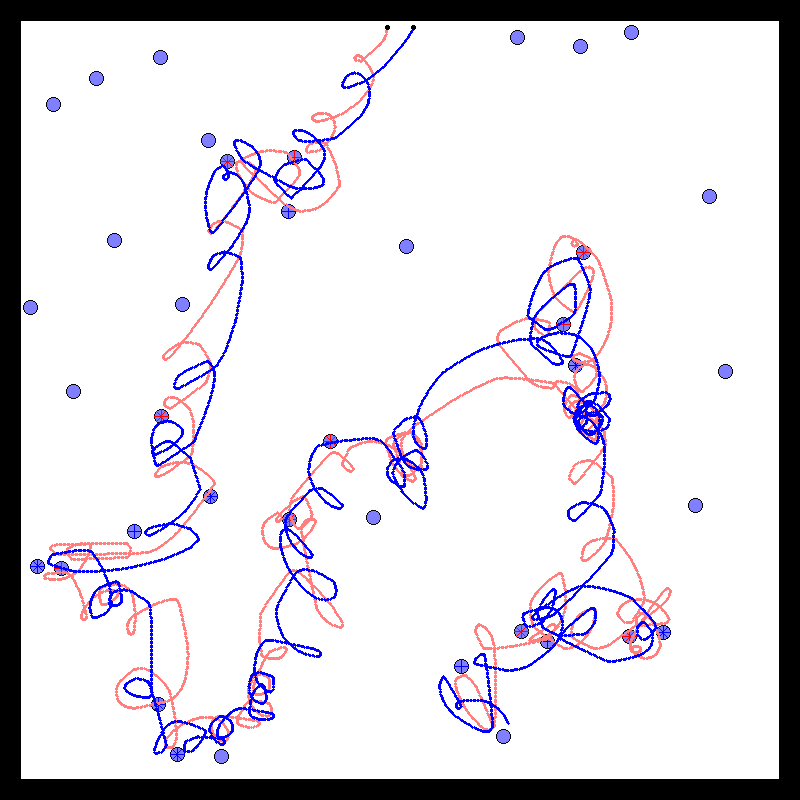
\includegraphics[scale=0.25]{fig/ArticleRob2/behaviorTurning.png}}
      \end{subfigure}~
      \begin{subfigure}[]
        {\label{fig:behaviorLeadership} 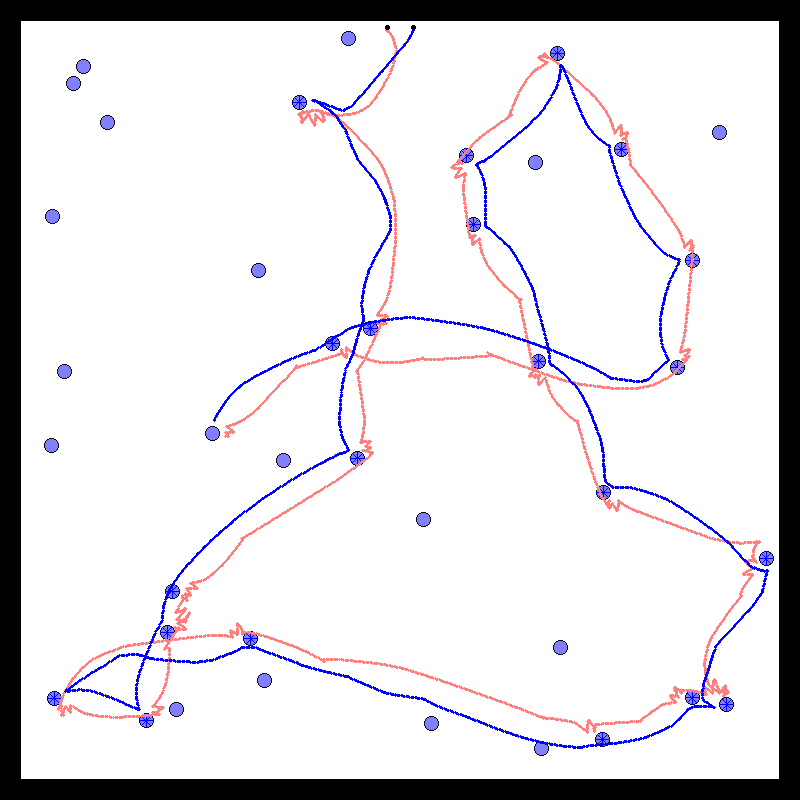
\includegraphics[scale=0.25]{fig/ArticleRob2/behaviorLeadership.png}}
      \end{subfigure}
      \caption{\textbf{Snapshots of the simulation after an entire trial in the foraging task.} The path of each robotic agent from their initial positions (black dots) is represented in red and blue. The blue discs represent the 18 targets in the environment. When a target is foraged by the two agents, a red cross (resp. blue) is drawn on the target if the red agent (resp. blue) arrived on it first. Each snapshot corresponds to a trial where agents adopted a different strategy: {\em (a)}~turning or {\em (b)}~leader/follower.}
      \label{fig:behaviorTraces}
  \end{figure}

  In the turning strategy, both individuals turn around one another so that they can keep the other individual in their line of sight and stay close to it (see Figure \ref{fig:behaviorTurning}). At the same time, the two individuals try to get closer to a target. This way, as soon as one of the two individuals is in contact with a target, the other individual can join it so the target may be collected cooperatively. Consequently, both individuals adopt a similar behaviour in this strategy and can be described as generalists.

  In the leader/follower strategy, the individuals specialise in two roles: a leader and a follower. The leader always gets on the target first and checks rarely for its partner. In comparison, the follower tries to keep its leader in view during the entirety of the simulation so that it can get on the same target (see Figure \ref{fig:behaviorLeadership}). Consequently, we observe the expression of two clearly heterogeneous behaviours which implies that both individuals are specialists. More importantly we also showed that, given our agents' capabilities, each phenotype needed to be encoded by a different genotype for specialisation to happen.

  \begin{figure*}[ht]
    \centerfloat
      \begin{subfigure}[]
        {\label{fig:Efficiency} 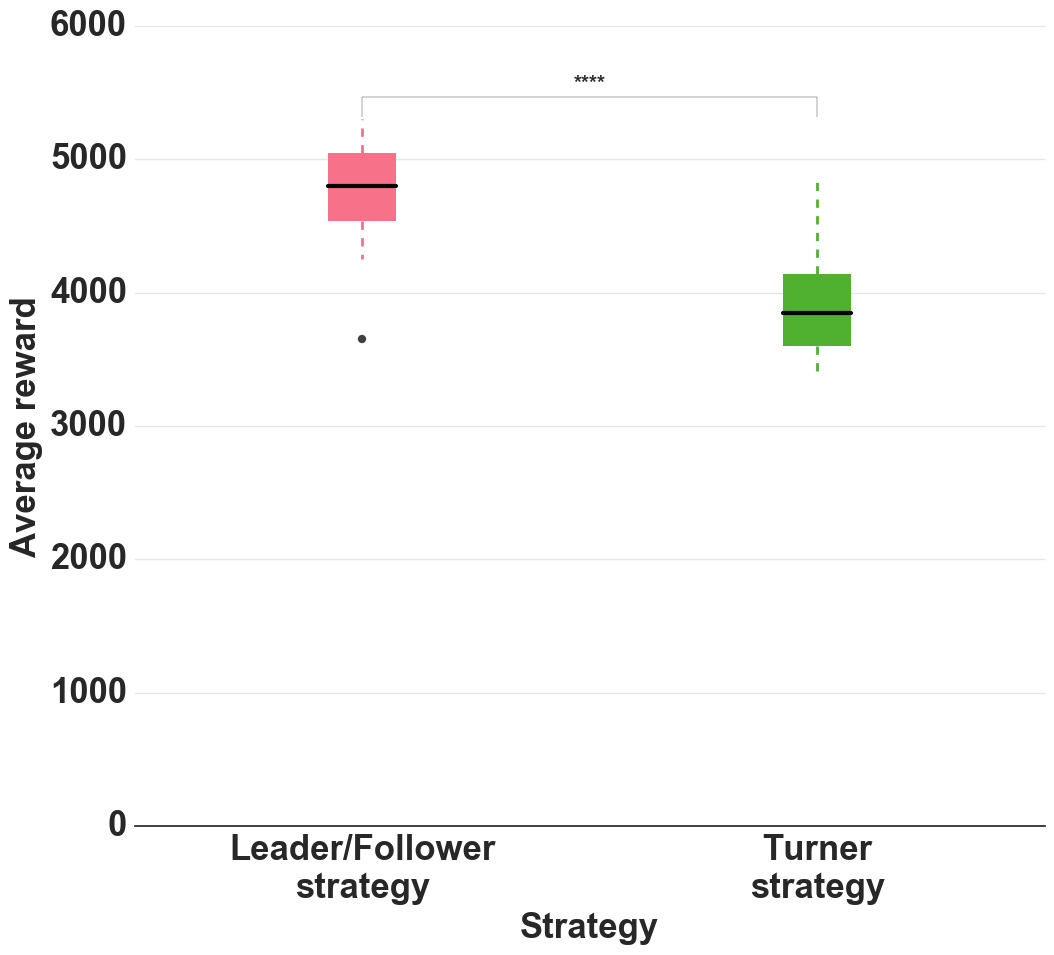
\includegraphics[scale=0.28]{fig/ArticleRob2/boxplotFitness.png}}
      \end{subfigure}~
      \begin{subfigure}[]
        {\label{fig:Leadership} 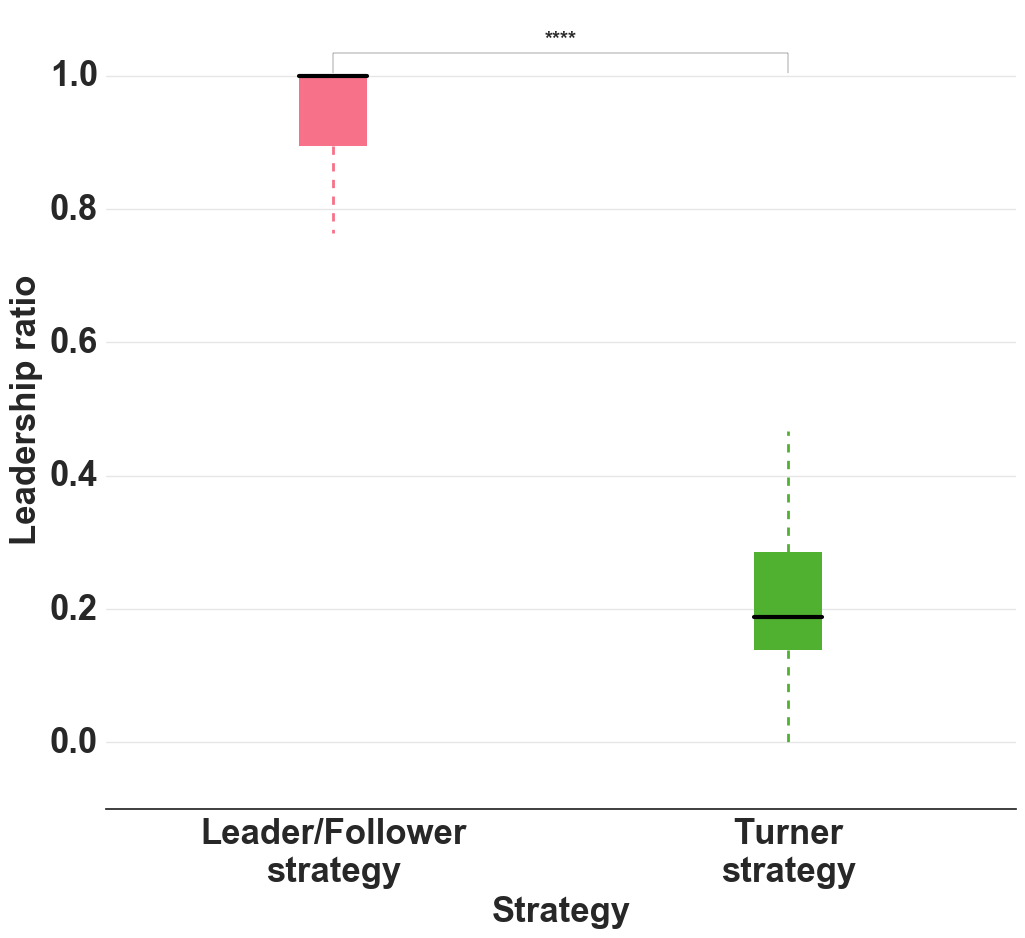
\includegraphics[scale=0.28]{fig/ArticleRob2/boxplotLeadership.png}}
      \end{subfigure}
      \caption{\textbf{Average reward and leadership proportion with a leader/follower or turning strategy} Boxplots of {\em (a)}~the average reward and {\em (b)}~the leadership proportion over $20$ independent trials for the leader/follower and turning strategies. The leadership ratio of an individual represents the propensity for one individual among the pair to arrive first more often than its partner on a target collected in a cooperative fashion. The position of each target at the beginning of each trial was randomized.}
      \label{fig:EfficiencyAndLeadership}
  \end{figure*}

  Figure~\ref{fig:Efficiency} shows the efficiency of each strategy, defined as the average reward obtained by the two individuals during a simulation over $20$ independent trials (with randomized targets' positions for each trial). We can see that, as expected, the leader/follower strategy achieves a significantly higher efficiency (Mann-Whitney U-test on the average reward over $20$ trials, {\em p}-value $< 0.0001$). This difference in efficiency is directly correlated to a highly significant difference in the proportion of leadership as shown in Figure~\ref{fig:Leadership} (Mann-Whitney U-test on the leadership proportion over $20$ trials, {\em p}-value $< 0.0001$). We compute this proportion by looking at the propensity for one of the two individuals to arrive first more often on a target foraged cooperatively (i.e. the emergence of a leader).



\section{Evolving Heterogeneous Behaviours with an Elitist Selection}
\label{sec:elitistEvolution}
  \subsection{Bootstrapping leader/follower strategies}
    In this first experiment, we are interested in the emergence of a leader/follower strategy when starting with a population of random individuals under an \((\mu + \lambda)\) elitist selection. In order to investigate the influence of population size, we tested three different sizes \(N\): $20$, $40$ and $100$. For each population size, we conducted $11$ independent runs, each one lasting $90000$ evaluations. For each population size \(N\), we defined \(\mu\) (i.e. the number of parents) and \(\lambda\) (i.e. the number of offsprings) as \(\frac{N}{2}\). For example, when population size was $100$, $50$ individuals were kept from the previous generation and used to create $50$ mutated offsprings.

    \begin{table}[ht]
      \center{
        \begin{tabular}{lcccc}
          \hline
          \textbf{Pop.} & \textbf{\# L/F} & \textbf{\# Turning} & \textbf{\# NC} & \textbf{Total}\\ 
          \textbf{size} & \textbf{Strat.} & \textbf{Strat.} & \textbf{Strat.} & \\ 
          \hline
          \textit{20} & 0 & 11 & 0 & \textbf{11}\\
          \textit{40} & 0 & 11 & 0 & \textbf{11}\\
          \textit{100} & 1 & 10 & 0 & \textbf{11}\\
          \hline
        \end{tabular}
      }
      \caption{\textbf{Strategies evolved by the best individuals under elitist selection with an initially random population.} Repartition of the different strategies adopted by the best individuals at the last evaluation in each of the replicates for different population sizes \(N\). We indicate in each cell the number of simulations where a particular strategy evolved. Populations were evolved under an \((\mu + \lambda)\) elitist selection, with \(\mu = \frac{N}{2}\) and \(\lambda = \frac{N}{2}\). Individuals' genotype values were intially random. In the table "L/F" stands for leader/follower and "NC" for "Non-Cooperative".}
      \label{tab:elitistScratchStrategies}
    \end{table}

    Table~\ref{tab:elitistScratchStrategies} shows the repartition of the best individuals' strategies at the last generation of evolution for each population size. We consider a behaviour to be cooperative when more than 50\% of the total number of targets collected are foraged cooperatively. First, we observe that in every replicate individuals always end up evolving a cooperative strategy. We also see that evolving a leader/follower strategy is difficult as specialists evolve in only $1$ run (out of $33$) and when the population size is $100$. These results suggest that it is nearly impossible to evolve such heterogeneous behaviours with this setting.

    \begin{figure}[ht]
      \centering
        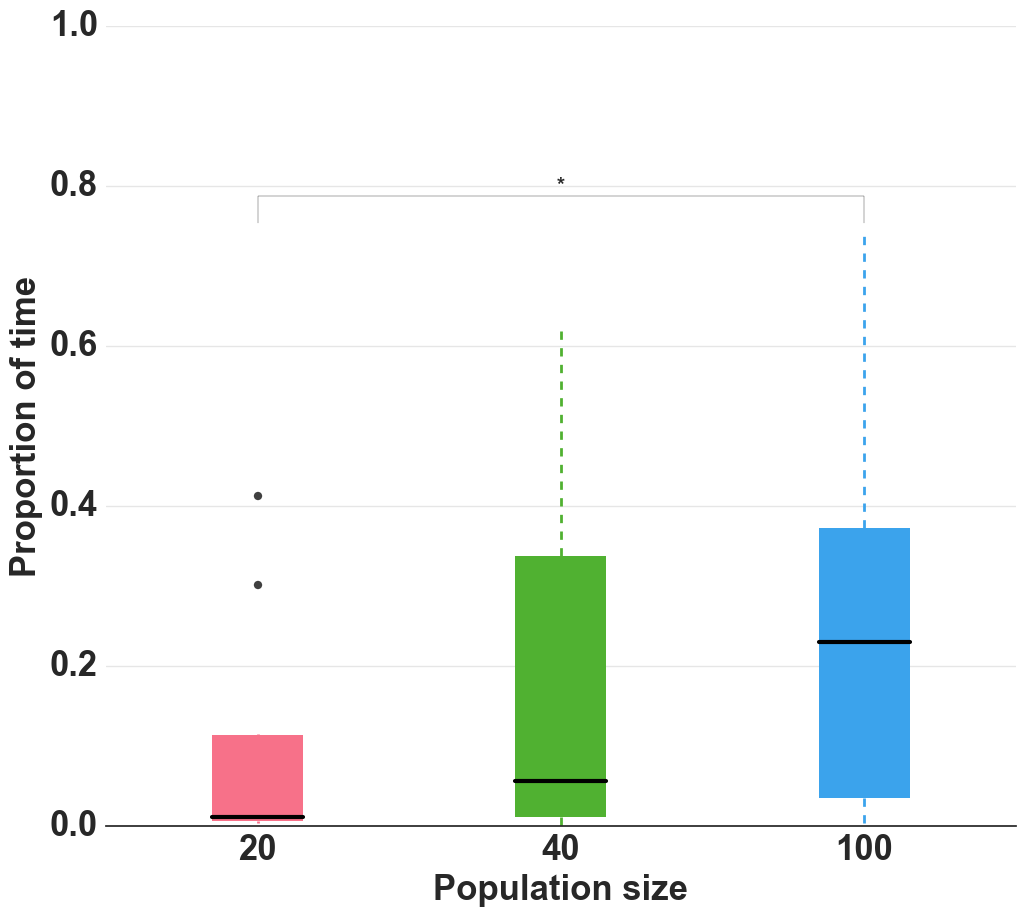
\includegraphics[scale=0.35]{fig/ArticleRob2/boxplotLeadershipTime.png}
        \caption{\textbf{Proportion of time with a leader/follower strategy.} Boxplots of the number of generations where the best individual in each replicate adopted a leader/follower strategy out of the total number of generations. We consider that the best individual adopted a leader/follower strategy when its leadership ratio was over a threshold value of $0.6$.}
      \label{fig:leadershipTime}
    \end{figure}

    However, when looking at the whole evolutionary history we can reveal additional information about the evolution of specialists. We show in Figure~\ref{fig:leadershipTime} the proportion of evolutionary time when the best individual of each run adopted a leader/follower strategy. This value is computed as the ratio of the number of generations when the leadership ratio was high enough (over a threshold value of $0.6$) out of the total number of generations. We observe that even if the best individuals end up adopting a generalist strategy, this was not the case during the entirety of the evolution. In particular, there is a significant increase (Mann-Whitney, {\em p}-value $< 0.05$) in the number of generations where the best individual showed a leader/follower strategy when population size was $100$ compared to a population size of $20$. Therefore this implies that it is possible to evolve specialists but their stability in the population over time is nearly impossible to achieve.


  \subsection{Maintaining heterogeneity in a population seeded with specialists}
    In order to investigate the lack of stability of genotypic polymorphism under elitist selection, we design another experiment. We separately evolve a population of efficient \emph{leader individuals} and \emph{follower individuals} beforehand. We then replace the worst individuals w.r.t. fitness score in the population of leaders by a certain amount of followers. Our goal is to study if artificially constructing such population could result in the invasion and fixation of a stable leader/follower strategy.

    The number of followers initially inserted in the population was varied according to two different settings: (1) we add only one follower or (2) we add an amount of followers equal to half of the population. Experiments were replicated $11$ times during $90000$ evaluations with population size of $40$ and $100$.

    \begin{table}[ht]
      \center{
        \begin{tabular}{lrcccc}
          \hline
          \textbf{Pop.} & \textbf{Followers} & \textbf{\# L/F} & \textbf{\# Turning} & \textbf{\# NC} & \textbf{Total}\\ 
          \textbf{size} & \textbf{added} & \textbf{Strat.} & \textbf{Strat.} & \textbf{Strat.} & \\ 
          \hline
          \textit{40} & \textit{1} & 0 & 11 & 0 & \textbf{11}\\
          \textit{40} & \textit{20} & 0 & 11 & 0 & \textbf{11}\\
          \textit{100} & \textit{1} & 1 & 10 & 0 & \textbf{11}\\
          \textit{100} & \textit{50} & 2 & 9 & 0 & \textbf{11}\\
          \hline
        \end{tabular}
      }
      \caption{\textbf{Strategies evolved by the best individuals under elitist selection when adding followers.} Repartition of the different strategies adopted by the best individuals at last evaluation in each of the replicates for different population sizes \(N\). We indicate in each cell the number of simulations where a particular strategy evolved. Populations were evolved under a \((\mu + \lambda)\) elitist selection, with \(\mu = \frac{N}{2}\) and \(\lambda = \frac{N}{2}\). The population was initially seeded with a population of leaders in which we added a specific amount of followers. In the table "L/F" stands for leader/follower and "NC" for "Non-Cooperative".}
      \label{tab:elitistInvasionStrategies}
    \end{table}


    We show (Table~\ref{tab:elitistScratchStrategies}) no significant differences in comparison to simulations with a population constituted of initially random individuals w.r.t. the number of simulations where a leader/follower strategy evolved. These results suggest that even when purposely adding specialists, their stability in the population is still very hard to achieve. This implies that whether the behaviours are evolved from random genotypes or bootstrapped with efficient individuals is not as important as maintaining heterogeneity in the population. In particular, in only one replicate among the $3$ runs where a leader/strategy was eventually adopted (out of $44$) did the specialists initially added were maintained. In the $2$ other runs we observe multiple emergences and disappearances of specialists throughout evolution. 


\section{Evolution Under a Fitness-Proportionate Selection}
\label{sec:fitpropEvolution}
  In this next experiment we want to investigate the evolution of heterogeneous behaviours when using a fitness-proportionate selection. As fitness-proportionate is known to allow frequency-dependent selection, we hypothesize that it may facilitate the evolution of specialists.

  \subsection{Bootstrapping leader/follower strategies}
    Similarly to the elitist selection, we replicated our experiments in $11$ independent runs during $90000$ evaluations. Likewise, population sizes were $20$, $40$ and $100$. 
    
    \begin{table}[ht]
      \center{
        \begin{tabular}{lcccc}
          \hline
          \textbf{Pop.} & \textbf{\# L/F} & \textbf{\# Turning} & \textbf{\# NC} & \textbf{Total}\\ 
          \textbf{size} & \textbf{Strat.} & \textbf{Strat.} & \textbf{Strat.} & \\ 
          \hline
          \textit{20} & 0 & 1 & 10 & \textbf{11}\\
          \textit{40} & 0 & 1 & 10 & \textbf{11}\\
          \textit{100} & 1 & 2 & 8 & \textbf{11}\\
          \hline
        \end{tabular}
      }
      \caption{\textbf{Strategies evolved by the best individuals under fitness-proportionate selection with an initially random population.} Repartition of the different strategies adopted by the best individuals at the last evaluation in each of the replicates for different population sizes. We indicate in each cell the number of simulations where a particular strategy evolved. Populations were evolved under a fitness-proportionate selection. Individuals' genotype values were initially random. In the table "L/F" stands for leader/follower and "NC" for "Non-Cooperative".}
      \label{tab:fitpropScratchStrategies}
    \end{table}

    We show in Table~\ref{tab:fitpropScratchStrategies} that results are highly different when using such selection scheme. In particular, the fitness-proportionate selection performed poorly w.r.t. evolving cooperative strategies. For each population size, no cooperative strategy evolved at all in the vast majority of replicates. However in one particular run we do observe the emergence and fixation of specialists. This is similar to what was observed under elitist selection w.r.t. evolving specialists.

    Yet a closer look at the dynamics of evolution under a fitness-proportionate selection yields interesting results. In particular, there is not much variation in the strategy adopted by the best individuals throughout evolution. This is consistent with the fact that the bootstrap of a cooperative strategy was not observed in most of the replicates: fitness-proportionate is not efficient in evolving any cooperative behaviour. In consequence, there is not much variation in the proportion of individuals adopting a leader/follower strategy during evolution. As a matter of fact, we observe that in the only replicate where there was genotypic polymorphism at the end of the simulation, specialists were already present at the random initialisation of the population and did not evolve through mutation. This is very different with the elitist selection where we observe multiple emergences of specialists (even briefly) during evolution in many different runs.

  \subsection{Maintaining heterogeneity in a population seeded with specialists}
    \begin{table}[ht]
      \center{
        \begin{tabular}{lrcccc}
          \hline
          \textbf{Pop.} & \textbf{Followers} & \textbf{\# L/F} & \textbf{\# Turning} & \textbf{\# NC} & \textbf{Total}\\ 
          \textbf{size} & \textbf{added} & \textbf{Strat.} & \textbf{Strat.} & \textbf{Strat.} & \\ 
          \hline
          \textit{40} & \textit{1} & 7 & 0 & 4 & \textbf{11}\\
          \textit{40} & \textit{20} & 8 & 0 & 3 & \textbf{11}\\
          \textit{100} & \textit{1} & 10 & 0 & 1 & \textbf{11}\\
          \textit{100} & \textit{50} & 10 & 0 & 1 & \textbf{11}\\
          \hline
        \end{tabular}
      }
      \caption{\textbf{Strategies evolved by the best individuals under fitness-proportionate selection when adding followers.} Repartition of the different strategies adopted by the best individuals at the last evaluation in each of the replicates for different population sizes \(N\). We indicate in each cell the number of simulations where a particular strategy evolved. Populations were evolved under a fitness-proportionate selection. The population was initially seeded with a population of leaders in which we added a specific amount of followers. In the table "L/F" stands for leader/follower and "NC" for "Non-Cooperative".}
      \label{tab:fitpropInvasionStrategies}
    \end{table}

    As expected from previous results, fitness-proportionate performs well in terms of stability of heterogeneous behaviours. We show in Table~\ref{tab:fitpropInvasionStrategies} that in the majority of replicates the best individuals adopt a leader/follower strategy at the end of the simulations. This is particularly true when population size is high enough ($100$). A major difference with the elitist selection is that in all replicates where a leader/follower strategy was observed at the end of the run, the specialists were maintained from the start throughout evolutionary time. These results suggest that, although not efficient at bootstrapping cooperative behaviours, fitness-proportionate performs well w.r.t. the stability of genotypic heterogeneity. Furthermore, we can hypothesize that this selection scheme is good at maintaining heterogeneity specifically because it largely fails (under our choice of parameters) at bootstrapping any cooperative strategy.


\section{Computational Analyses of Population Dynamics}
  In this present section, our goal is to understand more deeply the dynamics at play which allow the invasion of suboptimal generalists even when efficient specialists are present. To that end we run computational analyses based on the expected fitness of each of the three phenotypes. Table~\ref{tab:payoffMatrix} shows the average payoff of pair-wise simulations between each type of phenotypes. We consider the payoffs for both phenotypes in each pair to be identical as no significant differences were observed between their payoffs.

  \begin{table}[h]
    \center{
      \begin{tabular}{cccc}
        \hline
        \textbf{Phenotype} & \textit{Leader} & \textit{Follower} & \textit{Turner} \\
        \hline
        \textit{Leader} & 1265 & 5000 & 3480 \\
        \textit{Follower} & 5000 & 100 & 2750 \\
        \textit{Turner} & 3480 & 2750 & 2755 \\
        \hline
      \end{tabular}
    }
    \caption{\textbf{Payoff matrix for pair-wise simulations of each phenotype.} Average payoffs of each phenotype against every phenotype in a pair-wise simulation. Each pair was evaluated $10$ times in order to decrease the stochastic effects of the initial conditions (i.e. random positions of the targets).}
    \label{tab:payoffMatrix}
  \end{table}

  Several observations can be made directly from these results. First, we can confirm that the leader/follower strategy displayed by a (\emph{leader}, \emph{follower}) pair is clearly the best strategy. However each one of these two phenotypes performs very poorly against itself with the worst payoff obtained by a pair constituted of two \emph{followers}. Secondly, \emph{turner} individuals perform also very well against \emph{leaders}. Last, there is no significant differences w.r.t. payoffs when a \emph{turner} is paired with a \emph{follower} or another \emph{turner}. These last two points hint at a shared lineage between \emph{followers} and \emph{turners}. 

  Indeed analyses of the genotypes' histories in our previous experiments reveal that \emph{turner} individuals in fact descend from \emph{follower} individuals. This means that they act as \emph{followers} when interacting with \emph{leaders} but are not as efficient. However they are a lot more efficient than \emph{followers} when paired with individuals of the same phenotype (or \emph{followers}).

  % TODO: Virer le paragraphe précédent ? (notamment pour faire un peu de place)

  From this payoff matrix, we run computational analyses to model the gradient of phenotypes' repartition in an infinite population. The fitness \(W\) of a particular phenotype \(i\) is computed as follows:

  \[
    W_{i} = \sum_{j=1}^{M} P(ij)*F(j)
  \]

  with \(j\) the phenotype it is paired with, \(M\) the number of different phenotypes ($3$), \(P(ij)\) the payoff of phenotype \(i\) against \(j\) and \(F(j)\) the proportion of phenotype \(j\) in the population. From this fitness, we can deduce the variation of phenotypes repartition by updating the proportion \(F\) of each phenotype \(i\): 

  \[
    F_{i} = F_{i}*\frac{W_{i}}{\sum_{j=1}^{M} W_{j}}
  \]

  We show in Figure~\ref{fig:expectations} a vector field of this gradient. We can see that there actually exists an equilibrium between the three phenotypes (marked by the a dot at the crossing between the the dotted lines). This implies that even though the \emph{turner} strategy is not the more efficient one, it is still expected that this phenotype can invade and coexist with the two other phenotypes.

  We can hypothesize that we could not observe this equilibrium in our robotic simulations because of the stochastic effects arising from selection in a finite population. In order to study this hypothesis we ran additional computational simulations based on the same payoff matrix. The initial population is entirely composed of \emph{leaders} and the selection method is an elitist (\(\frac{N}{2}\)+\(\frac{N}{2}\)) evolution strategy where \(N\) is the population size. Every $10$ generations, each offspring has a probability of \(1*10^{-2}\) to mutate into any of the two other phenotypes.

  \begin{figure*}[ht]
    \centerfloat
      \begin{subfigure}[]
        {\label{fig:expectations} 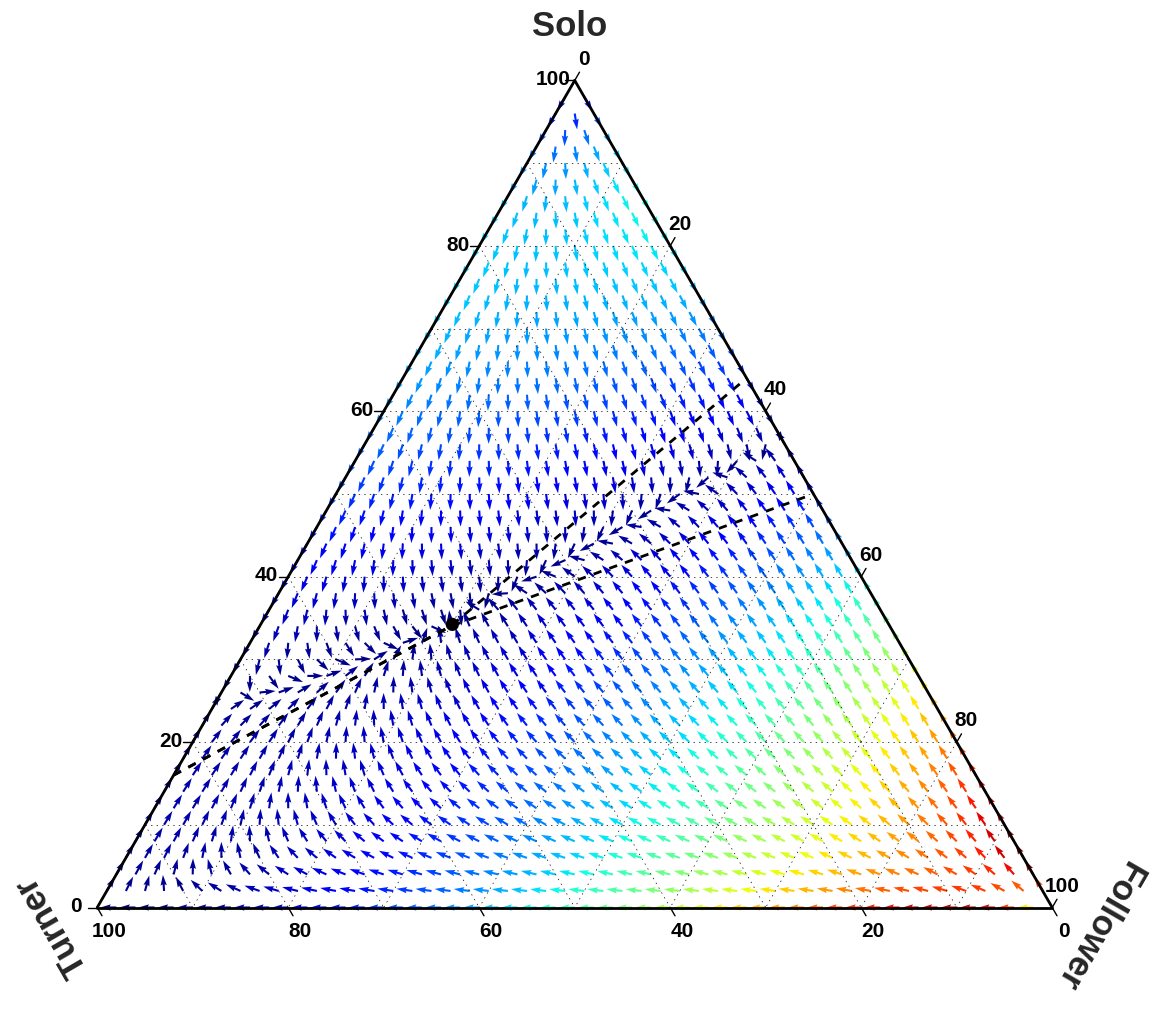
\includegraphics[scale=0.26]{fig/ArticleRob2/ExpectationsVectorsNormalized.png}}
      \end{subfigure}
      \begin{subfigure}[]
        {\label{fig:expectationsScatter} 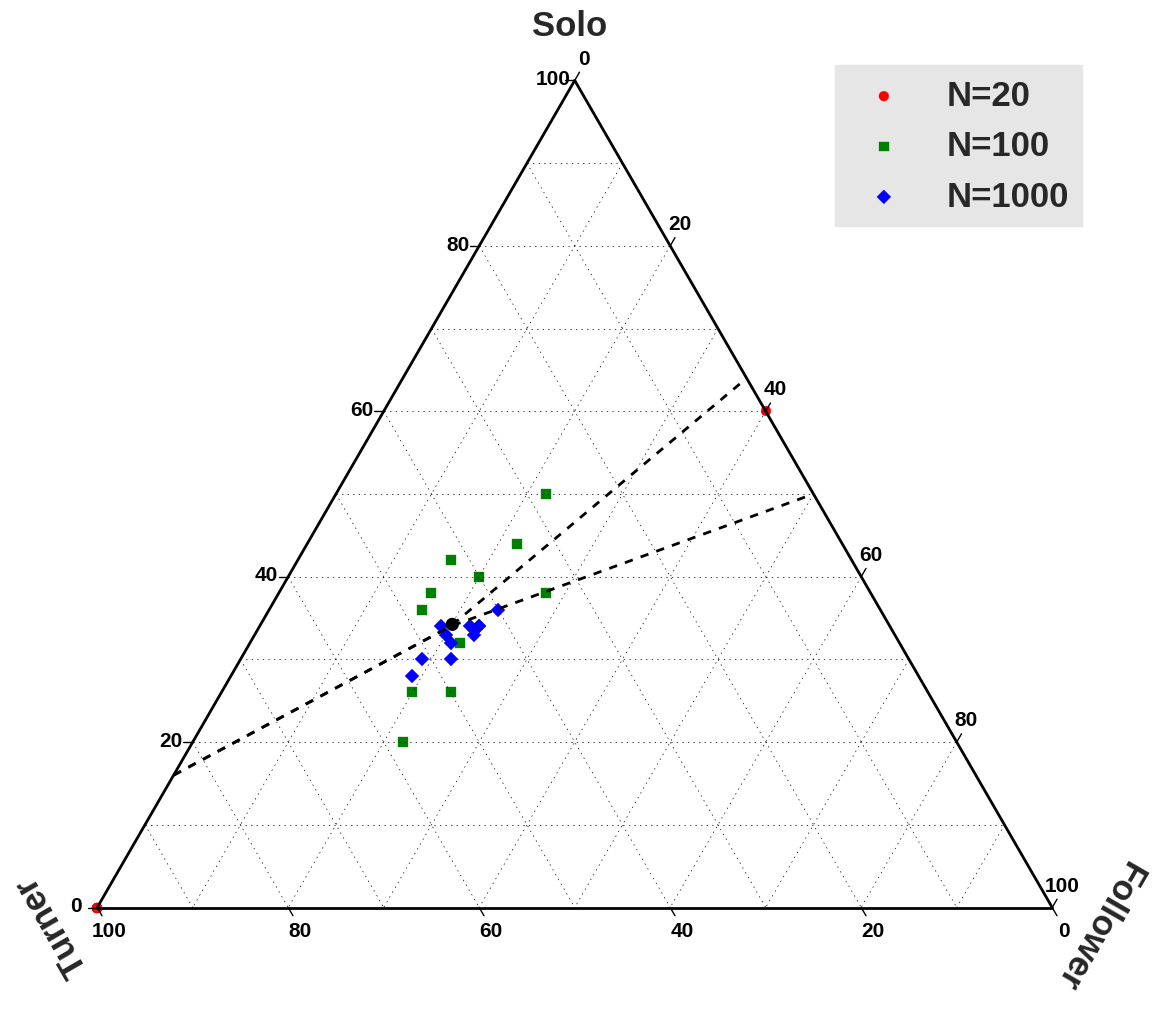
\includegraphics[scale=0.26]{fig/ArticleRob2/ExpectationsScatter.png}}
      \end{subfigure}
      \caption{\textbf{Vector field of the gradient of phenotypes' proportions and proportions of phenotypes at last generation of evolution.} {\em (a)}~Vector field of the gradient of phenotypes' proportions in an infinite population. The strength of variation is indicated by the color of the arrow. {\em (b)}~Repartition of phenotypes at the last generation of evolution for all three population sizes. Evolution lasted $1500$ generations and results were replicated across $11$ independent simulations. The initial population was entirely composed of \emph{leaders}.}
      \label{fig:ternary}
  \end{figure*}

  Figure~\ref{fig:expectationsScatter} shows the final repartition of phenotypes after $1500$ generations of evolution for \(N=20\), \(N=100\) and \(N=1000\) in $11$ independent replicates. We can see that when increasing population size we also increase the probability that an equilibrium where the three phenotypes exist is reached. We actually observe that the repartition of phenotypes at last generation of evolution gets closer to the predicted equilibrium as population size increases. This implies that when population size increases, the probability to lose particular phenotypes decreases. In other words, the effect that the stochasticity of fitness evaluation has on the sampling of the genotypes for the next generation is mitigated: population size is essential to the maintenance of specialists.


\section{Key Properties for Evolving Heterogeneous Behaviours}
  From the previous Section, we can hypothesize two key properties for the successful evolution of genotypic polymorphism. First, we showed that population size needed to be large enough in order to decrease the probability that heterogeneity could be lost during the evolutionary time. Even under an elitist selection where the best individuals are immediately selected, the stochastic nature of fitness evaluation entails that there is no guarantee that both types get selected. This means that a performance biased selection may lead to the composition of the new population not accurately representing the genotypic diversity of the previous one. Therefore, there needs to be a mechanism for the preservation of genotypic diversity. Second, we previously saw that one key reason for the invasion of \emph{turner} individuals is that, while \emph{followers} perform badly against themselves, this is not the case for the formers. This means that the manner in which robots are paired is essential for achieving specialisation.

  In order to test these hypotheses we design a last experiment where we diverge from the initial problem and now coevolve two separate populations. In this coevolution algorithm, each individual of one population is always evaluated against an individual of the other population ($5$ times as in previous experiments). Then, each population separately undergoes selection under an elitist \((10+10)\) selection method to create the population of the next generation (which means that each population size is $20$). We conducted $11$ independent replicates which lasted $90000$ evaluations each. The populations were initially constituted of random individuals.

  \begin{table}[ht]
    \center{
      \begin{tabular}{cccc}
        \hline
        \textbf{\# L/F} & \textbf{\# Turning} & \textbf{\# NC} & \textbf{Total}\\ 
        \textbf{Strat.} & \textbf{Strat.} & \textbf{Strat.} & \\ 
        \hline
        11 & 0 & 0 & \textbf{11}\\
        \hline
      \end{tabular}
    }
    \caption{\textbf{Strategies evolved by the best individuals when coevolving two populations.} Repartition of the different strategies adopted bt the best individuals at the last evaluation in each of the $11$ replicates. We indicate in each cell the number of simulations where a particular strategy evolved. Two populations were coevolved under elitist selection and the individuals' genotype values were initially random. In the table "L/F" stands for leader/follower and "NC" for "Non-Cooperative".}
    \label{tab:coevoStrategies}
  \end{table}

  We show (Table~\ref{tab:coevoStrategies}) that when using coevolution, we always evolve specialists in every replicates. Moreover, this algorithm is highly stable as the heterogeneous behaviours that emerged were never lost during evolution in every replicates. This means that coevolution is highly efficient both for the bootstrap of a leader/follower strategy and its maintenance throughout evolution. Regarding our hypothesized properties, we can check that the coevolution algorithm respects both of them. Firstly, as populations are separatly coevolved, we make sure that performance-based selection does not accidentally lead to the disappearance of specialists. Thus we ensure that the populations' genotypic diversity is highly protected. Secondly, we create a very specific pairing between individuals. Indeed individuals inside the same population are never partnered with one another. This means that \emph{followers} are always paired with \emph{leaders}. As \emph{turners} thus possesses no fitness benefit over the other phenotypes, their invasion is prevented. The question is open as to how to endow an algorithm working on a single population with such properties.

\section{Discussion and Conclusions}
\label{sec:discussion}
  In this paper, we investigated the evolution of specialisation through a leader/follower strategy in a cooperative foraging task. Our goal was to reveal the difficulties that arise when trying to evolve genotypic polymorphism in a single population. To that end, we mainly studied the dynamics of evolution with two different selection methods: an \((\mu + \lambda)\) elitist evolution strategy and fitness-proportionate selection.

  We first showed that the long term evolution of a leader/follower strategy was nearly impossible with an elitist selection. However bootstrapping specialists was not a problem as we observed that they frequently emerged during evolution. The major obstacle was rather to maintain heterogeneity over evolutionary time. Indeed, even when adding efficient followers to a population of leaders to force the adoption of a leader/follower strategy, specialists couldn't be maintained. In comparison, the properties shown by the fitness-proportionate algorithm were quite the opposite. While it was almost not capable of evolving a leader/follower strategy (nor any other cooperative strategy), the fitness-proportionate selection demonstrated high stability. It was therefore capable of maintaining specialists when present. We thus revealed two critical properties for evolving heterogeneous behaviours in a single population: \emph{bootstrapping} these behaviours and \emph{maintaining} them throughout evolution.

  We then ran computational analyses and showed that while a pair of turners is indeed less efficient w.r.t. payoff than a pair of leader and follower, it is a lot more efficient than a pair of leaders or a pair of followers. As a result, these individuals can easily invade part of the population. Moreoever, we also showed that the maintenance of specialists was very sensible to population size. Performance biased selection can indeed affect heterogeneity in the composition of the next generation's population. Finally, a coevolution algorithm, which we showed to be always successful in evolving heterogeneous behaviours, solved both of these two problems with (1) \emph{specific partners selection} as pairs were constituted of individuals from different populations and (2) \emph{protection} of the behaviours evolved by applying selection separately on the two populations. While this algorithm is not concerned with genotypic polymorphism in a single population, it is useful to yield effective mechanisms which could be studied to solve our problem. 

  This raises several interesting perspectives on how to solve this problem. First, niche protection could prevent the disappearance of the efficient but unstable leader/follower strategy. As a matter of fact, coevolution is akin to a particular type of niches protection with $2$ niches. However, we intend to investigate how we could implement such mechanism without specifying the explicit number nor the organization of the niches. Rewarding diversity~\parencite{Lehman2008} is also known as an effective way to protect novel behaviours and could be another promising direction. In particular, a multiobjective algorithm on performance and diversity~\parencite{Doncieux2014}, by rewarding genotypic and phenotypic diversity, may protect evolved specialists.

  Secondly, we showed that because partners were chosen randomly among the population, it created the opportunity for a "parasitic" strategy to invade. An interesting direction for future works could be to investigate restrictions in the choice of partners. For example it would be compelling to investigate how the individuals could evolve to select their partner based on genotypic or phenotypic information.

\chapter{Discussion}

% \epigraph{\textit{This is the end. My only friend, the end.}}{--- \textup{Jim Morrison}}

\minitoc[n] % minitoc without title

The contributions of this thesis have been divided in two parts that, while they revolve around evolutionary robotics, are centered on very different problems. As such, we choose here to discuss and conclude on each part separately.

\section{Modeling the Evolution of Cooperation}

	\subsection{Contributions Synthesis}

		In the first part of this thesis we have been interested in the influence of coordination in the evolution of mutualistic cooperation. We focused in particular on the proximate explanations of coordination and their impact on the ultimate evolution of cooperation. Most studies centered on cooperation have often been dedicated to explaining the stability of altruistic behaviours. Mutualistic actions in comparison have usually been ignored. However, while mutually beneficial actions do not raise any issue of stability, the origin of this type of cooperative behaviours is not trivial. Because they require coordination, the spread of a cooperative behaviour from an initial population of solitary individuals remains an open question. We thus were interested in the boostrap of mutually beneficial cooperation.

		To that end, we used evolutionary robotics as our modeling framework. Because we were interested in the origin of cooperative actions rather than their stability, the modeling of mechanistic constraints is critical. Namely, the convergence to a cooperative solution is impacted by the availability of mutations, i.e. the possibility for a particular mutant to appear in the population. While classical models in evolutionary biology are of great help in understanding the dynamics of the evolution of cooperation, they make critical assumptions with regards to the convergence towards a cooperative solution. This is what has motivated our choice to use individual-based modeling and evolutionary robotics in particular as a modeling method. In particular, evolutionary robotics allows to model the mapping between genotype and phenotype and thus study the proximate mechanisms at play in the evolution of cooperation.

		In a first study, we focused on the impact of modeling the mechanics of behaviour in the evolution of mutualistic cooperation. To that end we took inspiration from the game theoretical model of the stag hunt and studied the transition from a solitary equilibrium (hare hunting) to a cooperative equilibrium (stag hunting). We first revealed that there is a drastic difference between the results predicted by classical models in game theory and what we observed in evolutionary robotics. With a classical model, the transition to stag hunting always occured. In comparison, with a model in evolutionary robotics, this transition was nearly impossible. Furthermore, we showed that even under maximal genetic relatedness (i.e. individuals were clones of each other), the evolution of cooperation was still unlikely. We thus revealed that the mechanistic constraints are critical for the origin of cooperation in the stag hunt game. The evolution of cooperation is faced with a chicken \& egg dilemma: for cooperation to be selected, it needs to be beneficial. Yet the success of the cooperative action requires that others evolved the capacity to coordinate, which is not beneficial on its own. If we assume that a single mutation can lead to the evolution of cooperation then we consider that the same mutation is responsible for both the modification of the preferred prey and the capacity to coordinate. We showed here that doing so hides part of the issue. Moreover we showed in our simulations that the individuals needed to evolve a complex behaviour in order to be able to coordinate. Therefore, it is necessary to take into account the mechanics of behaviours in order to fully understand the evolution of cooperation. This means that there is a need for complementary frameworks which model these mechanisms.

		In the second Chapter, we studied how the nature of coordination behaviours may impact the transition between collective equilibria. More precisely, we focused on the issue of selecting between multiple stable equilibria. When a collective equilibrium has emerged, no single mutant has a selective advantage to deviate from this equilibrium. As such, this raises the issue of the transition to the optimal equilibrium. Our goal was to study if individual selection alone could lead to the optimization of group-traits. To that end, we used a model of collective hunting where individuals could choose between two types of prey: boar (suboptimal prey) and stag (optimal prey). We revealed that the transition towards the optimal prey was impossible under simple environmental features (only one prey of each type). However, we revealed that results were highly different when more realistic assumptions about collective hunting are made. Surprisingly, when the environment was more complex ($9$ prey of each type), the switch to stag hunting could sometimes occur. Under such environmental conditions, it was necessary to collectively decide on which prey to hunt. This meant that the evolution of coordination was required to achieve cooperation. In consequence, each individual evolved the capacity to react to the other individual's behaviour. This meant that a mutant could indirectly change the behaviour of the group and thus lead to stag hunting. However, we observed that the coordination strategy evolved was a very symmetrical one where both individuals could adopt the same behaviour. We then increased the neural complexity of individuals. We showed that the transition to stag hunting was then highly facilitated. Furthermore, we revealed that individuals evolved a strongly asymmetrical coordination strategy through specialization: a leader/follower strategy. In this strategy, the follower only reacted to the behaviour of the leader which it tried to follow. This means that a mutation on the leader was sufficient to change the group's behaviour and thus reap the benefits of cooperative stag hunting. Additionally, we observed that this strategy was more efficient than the previous one. We thus revealed that the evolution of an individually adaptive strategy (because more efficient) led to the transition to the optimal collective behaviour. Therefore, we showed that it was possible for individual selection alone to explain the optimization of group traits.

		In both of these studies, we thus revealed the critical role of coordination in the evolution of cooperation. In consequence, we demonstrated that it is indeed necessary to take the mechanics of coordination behaviours into account in order not to neglect crucial aspects of the evolutionary dynamics. Additionally, we also presented a general mechanism for the evolution of cooperation in the stag hunt. The boar we introduced in our study on the selection of equilibria could act as an evolutionary pathway in the stag hunt. Namely, this prey can be hunted alone but rewards more when it is hunted cooperatively, which is a realistic expectation for hunting in the natural world. As such, coordination and cooperation can initially be bootstrapped on this prey (because it is not as risky as hunting stags). Then, we showed that when coordination was already evolved it was possible for individual selection to optimize the collective behaviour. In consequence, this could lead to the transition to the purely cooperative equilibrium: stag hunting.


	\subsection{Limits and Perspectives}

		\subsubsection{The evolution of communication}

			During this thesis, we have studied coordination strategies that did not require any direct communication between individuals. We wanted to study if coordination was possible without endowing individuals with communication capabilities. Indeed, we aimed at keeping the complexity of our robot model as low as possible so that we could focus on the basic mechanisms that could lead to the evolution of cooperation. More complex agents could beg the question of the role of the robots' capabilities on the observed phenomena. In particular, the goal behind the first part of our study was to compare classical models in evolutionary biology with modeling under an evolutionary robotics framework. As such, it was important that no particular design choice could alter the relevance of this comparison.

			We found that our robots were capable of coordination without any means of communication. Indeed, they could evolve a surprising behaviour which, while it was not the most efficient way to coordinate, allowed them to cooperate. In a way, we can make here a similar observation as Mitri and colleagues~\parencite{Mitri2009}. Namely, individuals could rely on indirect communication cues resulting from their embodiement. However we could also implement a more direct way for them to communicate. Communication is used in numerous different social species, among which we already gave the example of the spotted hyenas~\parencite{Drea2009a, Smith2010, Smith2012a}. They are capable of using signaling techniques and communication in order to achieve high level of coordination during collective hunting. As such, while the empasis of our second study was mainly put on division of labour, communication could deeply impact the nature of coordination behaviours. In consequence, we hypothesize that the evolution of communication strategies could affect the evolution of collective actions. Additionally, an interesting perspective would be to let the individuals evolve how to communicate from basic communication capabitilies (e.g. the broadcast of a simple signal). As such, this could lead to coevolutionary dynamics between communication strategies and coordination behaviours.

			Moreoever, the evolution of communication has already been studied in several works in evolutionary robotics. We already mentioned in Chapter~\ref{chapter:model} that some have been interested in the general evolution of communication between foraging robots~\parencite{Floreano2007}, information suppression~\parencite{Mitri2009} or the role of historical contingencies on the evolution of signaling strategies~\parencite{Wischmann2012}. As with the evolution of cooperation, few have been interested in the role of communication among unrelated individuals. A notable counterexample is the work of Solomon et al.~\parencite{Solomon2012} who modeled communication strategies between hyenas. However, the impact of communication on the origin of mutualistic actions has not been studied.


		\subsection{Cooperation between bigger groups of agents}

			Our initial inspiration was the game theoretical framework of the stag hunt. As such interactions take place between only a pair of individuals. However, it could be interesting to increase the number of agents and to study how the evolutionary dynamics would change. In particular, in our second study we have been interested the optimization of group-traits by way of individual selection. We showed that the transition between multiple equilibria could occur without any group-level mechanism. As we provided no evidence that our demonstration could be scaled up to more than two individuals, it could be argued that what we consider a group-trait is limited in this context. 

			However, we believe that similar results would be observed in larger groups of individuals. We even hypothesize that the results could be more explicit in this case. Let's imagine that we consider a scaled-up version of our study where interactions take place between $5$ agents. The stag would now require that the $5$ individuals cooperate together to reap the benefits of the hunt. Because the coordination of $5$ individuals is more challenging than that of a pair, the evolution of efficient coordination strategies would be even more favored. As such, the evolution of asymmetrical behaviours like the leader/follower should have a bigger impact on the transition towards the optimum. Indeed, it would be impossible for a single mutant to lead the group to stag hunting without an asymmetrical strategy. We ran preliminary experiments on increasing the number of agents in our simulation (with groups of $3$, $4$ or $5$ robots). However, as of today we are faced with the fact that, given our parameters, it is challenging for the robots to evolve an efficient coordination strategy.


		\subsection{Online evolution}

			An interesting continuation of our work would be to model the evolution of mutualistic cooperation in an environment-driven online paradigm. More precisely, in the classical framework of evolutionary robotics we use an offline evolutionary algorithm. This initially means that there is a separation between the design of a robot and its deployment; robots are evolved in a different environment that the one where they are used. In comparison, under an online paradigm evolution occurs directly in the operational environment. The field of embodied evolution~\parencite{Watson2002} was created in order to address this question and in particular the issue of transferability that stems from evolving robots in an offline manner. As such, embodied evolution is mainly concerned with design questions. In our case, it would be interesting to use online evolution as another manner in which to model evolutionary phenomena. 

			Environment-driven evolution conveys another concept. In classical ER, a fitness function is used to evaluate the performance of individuals and determine if they will produce offsprings. This is different from the biological definition of fitness, where fitness is an \emph{a posteriori} evaluation of the reproductive sucess of a given individual. As such, a more realistic approach to the modeling of evolution would be to require that the individuals meet with each other in order to exchange genetic material~\parencite{Bredeche2010}. This is the principle of environment-driven evolution. In consequence, a perspective would be to study the evolution of mutualistic cooperation under such paradigm.

			Few have focused on this aspect of biological modeling. Montanier and Bredeche investigated the evolution of altruism among a population of simulated robots under an online environment-driven algorithm~\parencite{Montanier2011, Montanier2013}. This way they could study the impact of genetical relatedness and dispersion on the emergence and stability of altruistic behaviours.


\section{Automatic Design of Collective Robots}

	\subsection{Contributions Synthesis}

		In the second part of this thesis our goal was to study the evolution of cooperation in evolutionary robotics. More precisely, we were interested in the impact of genetic team composition on the evolution of efficient coordination strategies in multirobot systems. Multirobot systems have multiple advantages in comparison to using a single robot among which robustness, efficiency and the capacity to achieve tasks that a single robot could not. However, because they require the control of several agents, they are also more challenging to design. In this context, multiple different architectures exist for multirobot systems and several ways to design the control of collective robots have been proposed. But while a popular and often efficient method has been to manually design the robots, there has been a strong interest in creating methods to automatically design them. Automatic design can lead to robots that better react to environmental changes and unknown environment. In this context, we focused on evolutionary robotics as an approach to the automatic design of distributed robots.

		An open issue when designing cooperative robots in evolutionary robotics is team composition. Namely, the robots that constitute a team can be homogeneous or heterogeneous, whether in terms of morphology or control. Here we focused on the influence of team composition on the control of agents only. The classical approach in evolutionary robotics has been to use an homogeneous group of robots, where every individual comes from the same genotype. However, it is argued that heterogeneity could lead to more diverse behaviours between robots and thus generate higher efficiency.

		In the first Chapter of this part, we compared homogeneous and heterogeneous approaches on two criteria: evolvability and efficiency. We designed a collective foraging task inspired by the stag hunt where the individuals could forage two types of ressources: one that could be foraged alone and an other more rewarding that needed to be collected cooperatively. In this context, we define evolvability as capacity of a particular method to evolve cooperators while efficiency corresponds to the performance of the cooperative solution w.r.t. ressources collected. We compared a clonal approach (i.e. where individuals are homogeneous) to two aclonal ones (i.e. where the composition is heterogeneous): one where individuals are taken from the same population and the other where they come from two separately coevolved populations. We revealed that there exists a tradeoff between evolvability, which is best achieved with the clonal approach and efficiency, where coevolution evolved more efficient cooperative strategies. In particular we showed that division of labour would systematically evolve with coevolution. In order to go beyond this tradeoff and improve each method on both criteria, we then added incremental evolution. The goal of incremental evolution is to decompose a complex task into several sub-tasks that are evolved separately in order to ease the learning process. In our case, we pre-evolved our individuals in a simpler cooperative task. We showed that while this produced no significant differences for the clonal approach, the evolvability of coevolution was greatly increased. In consequence we showed that an aclonal approach, coevolution, was the best method on both evolvability and efficiency. However, this increase in evolvability comes at the price of a pre-evolution step. We thus revealed a new tradeoff: coevolution may outperform a clonal approach but at the cost of additional computations.

		In the next Chapter, we focused on the evolution of specialization between heterogeneous individuals. We took a simpler task than that of the previous Chapter where cooperation is easy to evolve but efficient coordination strategies are favored. In this task, we showed that two coordination strategies could evolve: a turner strategy where both individuals are generalists and a leader/follower strategy where the two robots specialize. We thus wanted to study how division of labour could evolve between heterogeneous individuals at the level of the population. We thus studied the evolution of genotypic polymorphism, i.e. the coexistence of several different genotypes (encoding for diverse phenotypes) in a single population. We compared two selection schemes based on their capacity to achieve genotypic polymorphism: a \((\mu + \lambda)\) evolution strategy and fitness proportionate. We revealed that while specialists could easily evolve under an elitist selection they could rarely be maintained throughout evolution. In comparison, fitness proportionate easily maintained genotypic polymorphism but was not efficient at evolving specialists. In order to understand the evolutionary dynamics at play, we then ran computational analyses based on the expected fitness of each strategy (turner, leader or follower) against every other strategy. We showed that generalists could invade the population by benefiting from the fact that specialists needed to be paired with complementary specialists in order to be efficient. Additionally, we revealed that under small population sizes, genetic diversity in the population could be lost during selection thus leading to the disappearance of specialists. From these results, we extracted two key properties for the evolution of genotypic polymorphism: stability of genotypic diversity and protection against the invasion of cheaters. While we could not achieve genotypic polymorphism in our study, we argued that an algorithm validating these properties could achieve this goal.

	\subsection{Limits and Perspectives}

		\subsubsection{Diversity and novelty}

			A popular open issue in evolutionary robotics is about the selective pressures of evolutionary algorithms~\parencite{Doncieux2015a}. The view of evolution as an optimization process led to the majority of works in ER typically relying on using a performance-based fitness. This means that an evaluation of performance is used to drive the search process toward the desired solutions. However, it has been shown that this approach of ER may lead to premature convergence which restricts the range of behaviours evolved as well as select solutions which are efficient on the short term only~\parencite{Mouret2012a}. In comparison there has been a recent interest for methods that do not rely exclusively on performance. Lehman and Stanley~\parencite{Lehman2011} introduced \emph{novelty search} for searching the goal of a maze and the evolution of bipedal walk. Selection was based on the novelty of behaviours compared to previous solutions rather than performance. They showed that this led to better results thanks to a more extensive research through the space of behaviours than with performance-oriented fitness. Mouret \& Doncieux~\parencite{Mouret2012a} used a multi-objective approach to optimize on both performance and behavioural diversity. They showed that this led to improvements in comparison to a more classical performance-based search.

			In our case, we showed that there is a tradeoff between evolvability and efficiency. Aclonal approaches could evolve more efficient cooperative solutions but less easily than a clonal approach. Performance-based selection may in this case drive the evolutionary process to permaturely lose cooperative individuals as they are not efficient on their own. As such, multi-objective optimization on both diversity and performance could allow to maintain these individuals in the population and thus allow the evolution of cooperation. In our study on genotypic polymorphism, diversity could also be used in order to protect the evolution of specialists. In this case we expect a population of specialists to be more diverse (in terms of genotype and phenotype) than one constituted of generalists. As such diversity could allow to maintain the presence of division of labour in the population.

			Preliminary results of multi-objective optimization with diversity did not unfortunately produce satisfying results w.r.t. evolving cooperation. Diversity is not a magic trick that luckily happens to find novel solutions. One of the main challenges when using diversity is to find an efficient measure of behavioural distance. While we think that diversity could be helpful in our case, finding both a correct and sufficiently general measure of this distance in the case of cooperation is challenging.


		\subsubsection{The transfer to real robots}

			In every experiment in this manuscript, we used simulated robots. While we believe our findings to mostly contribute to theoretical knowledge and not to be constrained by a particular robot model, it still would be interesting to know how our results would apply to real robots. This perspective might relate to both parts of this thesis. However, in the case of modeling the evolution of cooperation, we would not learn more by using real robots rather than simulated ones. As previously explained, this would mostly ensure that no unrealistic physical assumptions are made in our simulations. We thus believe real robots to be more of an interesting perspective in our study of automatic design in evolutionary robotics.

			We could thus study the transferability of evolved solutions, which is an open issue in evolutionary robotics~\parencite{Mouret2012b, Doncieux2015a}. As we already mentioned, several assumptions are made when using simulations of robotic agents. While we model a sensory system for our robots, sensors in the real world are noisy. Also, friction can alter the way individuals move or collide with each others. As such, this creates a reality gap where evolved behaviours may not perform well when embedded in physical robots. This is one of the reasons behind the creation of embodied evolution~\parencite{Watson2002}, of which we previously talked about.

	    \begin{figure}[hbt]
	        \begin{center}
	          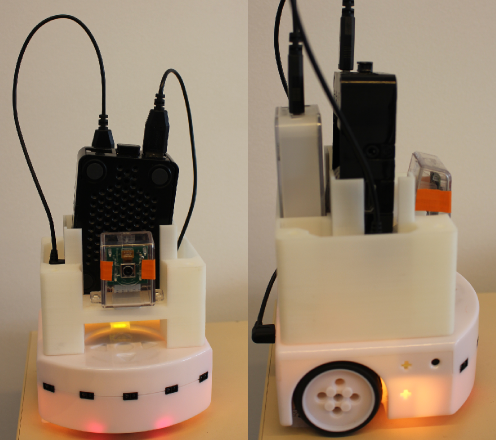
\includegraphics[scale = 0.50]{fig/Discussion/Robot.png}
	          \caption{\textbf{Physical robot for distributed robotics.}
	          Picture of a robot designed to be used for our experiments in distributed robotics. This robot is composed of a Thymio-II base which is equipped with two wheels and a collection of sensors, among which proximity sensors. A 3D-printed structure is used to support a raspberry PI, a camera module and a battery. The raspberry PI is used to have a more complex control of the Thymio.} 
	          \label{fig:thymioPicture}
	        \end{center}
	    \end{figure}

			During this thesis, we worked on the creation of a robotic platform for the control of collective robots. The goal was to use simple and cheap robots in order to address distributed robotics questions. We thus designed robots composed of a Thymio-II, a raspberry PI and a camera module for raspberry (see Figure~\ref{fig:thymioPicture}). The Thymio constitutes the base of the robots and is equipped with two wheels and a collection of proximity sensors. The raspberry acts as the controller of the Thymio and can be used to write instructions to the Thymio and read sensory inputs. Preliminary experiments on those robots showed that the evolved leader/follower strategy could transfer well in simple situations. Additional experiments are needed to really validate the transferability of our solutions.

			% Un peu plus sur EE ? Genre dire qu'on pourrait le faire


\section{Concluding Remarks}

	This present work aimed at contributing to the field of evolutionary robotics in two different ways: model and design~\parencite{Trianni2014b, Doncieux2015a}. On the one hand, we modeled the issue of the evolution of mutualistic cooperation. Thanks to evolutionary robotics we could show that the proximate explanations of behaviours are critical in understanding the origin of mutually beneficial actions. Thus we hopped to convince readers that there is an interest in using evolutionary robotics as a modeling framework in evolutionary biology and that a wide range of other phenomena could be adressed this way. On the other hand, we studied the automatic design of controllers for distributed robotics. We revealed that there are advantages in using heterogeneous teams of individuals and that it may be useful no to restort to the classical approach of evolving clonal controllers. Therefore we contributed to the open question of genetic team compositions in evolutionary robotics. In conclusion we believe that evolutionary robotics can indeed seriously contribute in one or the other way and that there is potential for scientific research in either direction..


\cleardoublepage % little hack for moving the side marker down
\stepcounter{fchapter}
%%%%%%%%%%%%%%%%%%%%%%%%%%%%%%%%%%%%%%%%%%%%%%%%%%%%
\chapter*{Publications}
\addstarredchapter{Publications}
\chaptermark{Publications}

\begin{refsection}

%% Articles
\nocite{Bernard2015, Bernard2016a, Bernard2016b}
% \nocite{Bernard2016a}
% \nocite{Bernard2016b}

\printbibliography[keyword=own,notkeyword=talk,
  heading=subbibliography,
  title={Articles}]

%% Talks
\nocite{BernardALife}
\nocite{BernardECAL}
\nocite{BernardJET}

\printbibliography[keyword=own,keyword=talk,
  heading=subbibliography,
  title={Invited talks}]

\end{refsection}



%%%%%
\renewcommand{\bibfont}{\small}
\printbibliography[notkeyword=unbib]

%%%%%
% \tableofglossaries

%%%%%
% \tableofindex

\end{document}
